% Options for packages loaded elsewhere
\PassOptionsToPackage{unicode}{hyperref}
\PassOptionsToPackage{hyphens}{url}
\PassOptionsToPackage{dvipsnames,svgnames,x11names}{xcolor}
\documentclass[
  11pt]{article}
\usepackage{xcolor}
\usepackage[a4paper,margin=2.5cm]{geometry}
\usepackage{amsmath,amssymb}
\setcounter{secnumdepth}{-\maxdimen} % remove section numbering
\usepackage{iftex}
\ifPDFTeX
  \usepackage[T1]{fontenc}
  \usepackage[utf8]{inputenc}
  \usepackage{textcomp} % provide euro and other symbols
\else % if luatex or xetex
  \usepackage{unicode-math} % this also loads fontspec
  \defaultfontfeatures{Scale=MatchLowercase}
  \defaultfontfeatures[\rmfamily]{Ligatures=TeX,Scale=1}
\fi
\usepackage{lmodern}
\ifPDFTeX\else
  % xetex/luatex font selection
  \setmainfont{DejaVuSerif.ttf}[BoldFont=DejaVuSerif-Bold.ttf,ItalicFont=DejaVuSerif-Italic.ttf,BoldItalicFont=DejaVuSerif-BoldItalic.ttf]
  \setsansfont{DejaVuSans.ttf}[BoldFont=DejaVuSans-Bold.ttf,ItalicFont=DejaVuSans-Oblique.ttf,BoldItalicFont=DejaVuSans-BoldOblique.ttf]
  \setmonofont{DejaVuSansMono.ttf}[BoldFont=DejaVuSansMono-Bold.ttf,ItalicFont=DejaVuSansMono-Oblique.ttf,BoldItalicFont=DejaVuSansMono-BoldOblique.ttf]
\fi
% Use upquote if available, for straight quotes in verbatim environments
\IfFileExists{upquote.sty}{\usepackage{upquote}}{}
\IfFileExists{microtype.sty}{% use microtype if available
  \usepackage[]{microtype}
  \UseMicrotypeSet[protrusion]{basicmath} % disable protrusion for tt fonts
}{}
\makeatletter
\@ifundefined{KOMAClassName}{% if non-KOMA class
  \IfFileExists{parskip.sty}{%
    \usepackage{parskip}
  }{% else
    \setlength{\parindent}{0pt}
    \setlength{\parskip}{6pt plus 2pt minus 1pt}}
}{% if KOMA class
  \KOMAoptions{parskip=half}}
\makeatother
\usepackage{color}
\usepackage{fancyvrb}
\newcommand{\VerbBar}{|}
\newcommand{\VERB}{\Verb[commandchars=\\\{\}]}
\DefineVerbatimEnvironment{Highlighting}{Verbatim}{commandchars=\\\{\}}
% Add ',fontsize=\small' for more characters per line
\newenvironment{Shaded}{}{}
\newcommand{\AlertTok}[1]{\textcolor[rgb]{1.00,0.00,0.00}{\textbf{#1}}}
\newcommand{\AnnotationTok}[1]{\textcolor[rgb]{0.38,0.63,0.69}{\textbf{\textit{#1}}}}
\newcommand{\AttributeTok}[1]{\textcolor[rgb]{0.49,0.56,0.16}{#1}}
\newcommand{\BaseNTok}[1]{\textcolor[rgb]{0.25,0.63,0.44}{#1}}
\newcommand{\BuiltInTok}[1]{\textcolor[rgb]{0.00,0.50,0.00}{#1}}
\newcommand{\CharTok}[1]{\textcolor[rgb]{0.25,0.44,0.63}{#1}}
\newcommand{\CommentTok}[1]{\textcolor[rgb]{0.38,0.63,0.69}{\textit{#1}}}
\newcommand{\CommentVarTok}[1]{\textcolor[rgb]{0.38,0.63,0.69}{\textbf{\textit{#1}}}}
\newcommand{\ConstantTok}[1]{\textcolor[rgb]{0.53,0.00,0.00}{#1}}
\newcommand{\ControlFlowTok}[1]{\textcolor[rgb]{0.00,0.44,0.13}{\textbf{#1}}}
\newcommand{\DataTypeTok}[1]{\textcolor[rgb]{0.56,0.13,0.00}{#1}}
\newcommand{\DecValTok}[1]{\textcolor[rgb]{0.25,0.63,0.44}{#1}}
\newcommand{\DocumentationTok}[1]{\textcolor[rgb]{0.73,0.13,0.13}{\textit{#1}}}
\newcommand{\ErrorTok}[1]{\textcolor[rgb]{1.00,0.00,0.00}{\textbf{#1}}}
\newcommand{\ExtensionTok}[1]{#1}
\newcommand{\FloatTok}[1]{\textcolor[rgb]{0.25,0.63,0.44}{#1}}
\newcommand{\FunctionTok}[1]{\textcolor[rgb]{0.02,0.16,0.49}{#1}}
\newcommand{\ImportTok}[1]{\textcolor[rgb]{0.00,0.50,0.00}{\textbf{#1}}}
\newcommand{\InformationTok}[1]{\textcolor[rgb]{0.38,0.63,0.69}{\textbf{\textit{#1}}}}
\newcommand{\KeywordTok}[1]{\textcolor[rgb]{0.00,0.44,0.13}{\textbf{#1}}}
\newcommand{\NormalTok}[1]{#1}
\newcommand{\OperatorTok}[1]{\textcolor[rgb]{0.40,0.40,0.40}{#1}}
\newcommand{\OtherTok}[1]{\textcolor[rgb]{0.00,0.44,0.13}{#1}}
\newcommand{\PreprocessorTok}[1]{\textcolor[rgb]{0.74,0.48,0.00}{#1}}
\newcommand{\RegionMarkerTok}[1]{#1}
\newcommand{\SpecialCharTok}[1]{\textcolor[rgb]{0.25,0.44,0.63}{#1}}
\newcommand{\SpecialStringTok}[1]{\textcolor[rgb]{0.73,0.40,0.53}{#1}}
\newcommand{\StringTok}[1]{\textcolor[rgb]{0.25,0.44,0.63}{#1}}
\newcommand{\VariableTok}[1]{\textcolor[rgb]{0.10,0.09,0.49}{#1}}
\newcommand{\VerbatimStringTok}[1]{\textcolor[rgb]{0.25,0.44,0.63}{#1}}
\newcommand{\WarningTok}[1]{\textcolor[rgb]{0.38,0.63,0.69}{\textbf{\textit{#1}}}}
\usepackage{longtable,booktabs,array}
\usepackage{calc} % for calculating minipage widths
% Correct order of tables after \paragraph or \subparagraph
\usepackage{etoolbox}
\makeatletter
\patchcmd\longtable{\par}{\if@noskipsec\mbox{}\fi\par}{}{}
\makeatother
% Allow footnotes in longtable head/foot
\IfFileExists{footnotehyper.sty}{\usepackage{footnotehyper}}{\usepackage{footnote}}
\makesavenoteenv{longtable}
\setlength{\emergencystretch}{3em} % prevent overfull lines
\providecommand{\tightlist}{%
  \setlength{\itemsep}{0pt}\setlength{\parskip}{0pt}}
\usepackage{tikz}
\usetikzlibrary{arrows.meta,positioning,shapes.geometric}
\usepackage{etoolbox}
\AtBeginEnvironment{longtable}{\footnotesize}
\setcounter{secnumdepth}{0}
\setcounter{tocdepth}{2}
\renewcommand{\contentsname}{Contents}
\sloppy
\setlength{\parskip}{2pt}
\usepackage{bookmark}
\IfFileExists{xurl.sty}{\usepackage{xurl}}{} % add URL line breaks if available
\urlstyle{same}
\hypersetup{
  colorlinks=true,
  linkcolor={NavyBlue},
  filecolor={Maroon},
  citecolor={Blue},
  urlcolor={NavyBlue},
  pdfcreator={LaTeX via pandoc}}

\author{}
\date{3 November 2026}

\begin{document}

\section{Sovereign Epistemic Acquisition: A Conditional Framework for
Active Information Acquisition and Sovereign Filtering under Bounded
Agency, with Pilot
Evidence}\label{sovereign-epistemic-acquisition-a-conditional-framework-for-active-information-acquisition-and-sovereign-filtering-under-bounded-agency-with-pilot-evidence}

\textbf{Wen Hu}1,2~~\textbf{Xutong Wang}1~~\textbf{Ya Yu}1

1 College of Electronic and Information Engineering, Nanjing University
of Aeronautics and Astronautics, Nanjing, China 2 Jiangsu Yunhefeng
Intelligent Technology Co., Ltd., Jiangsu, China

Corresponding author: Wen Hu (huwen@nuaa.edu.cn)

November 2026 · Human--AI collaboration (AI contributions disclosed in
the \emph{Human--AI Collaboration and AI Contribution Statement})

\begin{center}\rule{0.5\linewidth}{0.5pt}\end{center}

\subsection{Abstract}\label{abstract}

In an era in which the marginal cost of producing information approaches
zero, a bounded agent faces an arithmetic constraint: with a daily
cognitive budget \(T\) against a candidate supply \(N \sim 10^4\), the
filtering ratio must exceed 99.8\%. Today's filtering infrastructure
optimizes platform engagement rather than the agent's own ends---a
systemic abdication of epistemic sovereignty---while active acquisition
and passive filtering have been studied in isolation. This paper
proposes \textbf{Sovereign Epistemic Acquisition (SEA)}, which recasts
information acquisition as a unified optimization problem---the
Sovereign Acquisition Problem (SAP)---under the agent's second-order
objective and within its cognitive budget, with ownership of the filter,
its objective function, and its audit trail resting with the agent. Main
results: (i) a per-decision structural decomposition of expected
realized decision value under assumptions (V1)--(V5), with the
five-dimensional exact summary proved under sufficient representability
assumptions for all value, durability, credibility, and harm terms, not
inferred from their semantic names; (ii) a distribution-free
threshold/quantile identity and its equal-variance Gaussian
specialization showing that the stated document-level, single-score,
top-\(m\) model requires approximately \(d' \ge 4.39\) for 95\% recall
at the specified extreme filtering ratio---evidence for one sufficient
architectural remedy, not a proof that dual channels are necessary for
every architecture or for proposition-level recall; (iii)
redundancy-coverage theorems bounding miss probability by
\((1-p_{\min})^{k_{\mathrm{eff}}}\)---\textbf{conditionally tight}
bounds whose strength is exactly the institutional provenance of the
coverage floor \(p_{\min}\) (§7.7); (iv) a conditional KKT
characterization of attention allocation, including interior and corner
cases, with Pandora and patch rules compared only after conversion to a
common value unit; (v) a unified goal-capture model with firewall
bounds, human-gated virtue convergence (conditional convergence: the
zero-drift-floor branch is Theorem 10.1 only under strengthened
filtration-conditional and post-gate drift assumptions; the
positive-drift-floor branch is \textbf{a conjecture, not a theorem}
(Conjecture 10.1), supported by an ODE-method sketch with an explicit
verified/unverified checklist), pre-authorization regret bounds, and a
fragmentation lower bound for public agenda layers. This is a
framework/synthesis paper: the contribution is the structure and problem
formulation, not new general-purpose mathematical tools; each guarantee
is limited to its stated assumptions, and conditional design bounds and
conjectures are not represented as proved deployment guarantees.
Completed work comprises two-domain real-corpus pilots, data collection
for a four-family LLM-agent judgment-layer mechanistic replay, and its
controlled 17-scenario unique-key reanalysis, providing \textbf{pilot
support and applicability-boundary mapping, not population-level
validation}; legacy non-deduplicated outputs are distinguished from the
new within-corpus exploratory estimates, and neither constitutes
confirmatory inference. \textbf{Negative result stated up front: the
95\% target is rejected for the tested academic post-hoc citation proxy
(best proxy recall 0.28), which does not measure ex-ante critical
recall.} ``Pilot evidence'' in the title means mechanism checks and
applicability-boundary mapping, not general validation: \textbf{no
human-subject data have been collected to date}; all human-side
conclusions remain falsifiable predictions, and a minimal human
feasibility pilot (HP-0, \(n \le 10\), low intensity) is fully designed
and awaiting data collection (§15.5; see the Statement of Evidence
Status below).

\textbf{Keywords}: epistemic sovereignty; active information
acquisition; information filtering; value of information; adversarial
robustness; common knowledge

\textbf{Revision status (v1.8).} This major revision narrows the formal
and empirical claims after an independent read-only computational
replay-integrity audit. It introduces no new experiment or human-subject
data. Corrected statements and proofs supersede their v1.7 counterparts;
the pre-specified duplicate disposition, full unique-key reanalysis, and
17-scenario audit are complete and explicitly labeled controlled
within-corpus exploratory reanalysis after legacy results were seen.
Renewed human-author mathematical sign-off, leakage-resistant temporal
tests, and the planned S2d/S4/S5 baselines remain outstanding and are
not represented here as completed. The auditor-reported local Lean Web
checks are scoped below; this revision claims neither paper-wide Lean
certification nor independent reproduction of those checks.

\begin{center}\rule{0.5\linewidth}{0.5pt}\end{center}

\subsection{Statement of Evidence Status (Honest
Disclosure)}\label{statement-of-evidence-status-honest-disclosure}

Validation follows a three-tier architecture: LLM-agent cohorts serve as
the primary mechanistic testbed (synthetic ecologies and real-corpus
temporal replays), online public human data serve as transfer anchors,
and a human RCT protocol is fully archived but deferred. \textbf{All
human-side conclusions (virtue convergence, backfire protection,
calibration improvement, deskilling protection) are falsifiable
predictions, not established results; the population-level validation
(the full P1--P12 battery) is still in progress, and the pre-registered
sample sizes have not been reached.} Completed work comprises the
two-domain pilots, data collection for the four-family LLM-agent
judgment-layer mechanistic replay, and a controlled unique-key
reanalysis of that replay; all results remain within-corpus exploratory
and concern only the judgment-layer component (academic domain; four
families, 80 runs in total; 73,547 legacy valid rows but 71,914 valid
unique run/agent/sim\_day keys, plus 86 gaps (56 empty-only and 30
no-surviving-row): main rule A resolves 71,573 recall, 70,676 value, and
71,618 sign keys, yielding judgment-arm recall 0.443790--0.532600 versus
0.241 only as a fixed descriptive reference, positive Δrecall in every
family but an O interval crossing zero and O run-cluster p=0.1601,
Δvalue positive for C/Q and negative for O/G, and all McNemar/CMH
statistics demoted to nominal within-corpus sensitivity descriptions;
the controlled analysis is not prospective preregistration or
confirmatory evidence); and we report the negative results first: the
95\% target is rejected for the tested academic post-hoc citation proxy
(best proxy recall 0.28), which does not measure ex-ante critical
recall; the financial domain attains within-portfolio recall 0.952 under
highly favorable conditions (25 direct-pass holdings, 4.6
propositions/day, quota-feasible, post-hoc ground-truth proxy), diluted
to 0.910 after news-layer expansion (displayed proxy miss rate
4.8\%→9.0\%, +87.5\%; unrounded +89.47\%; the within-portfolio target
count changes from 18 to 19, so this is not a same-denominator paired
effect)---a recall of \emph{post-hoc} market-moving days, not of
\emph{ex-ante} critical information, with limited construct validity;
public-layer certification initially fails in the real news ecology and
only partially recovers to weak same-corpus enrichment (market-only lift
0.615→1.230; market∪legal lift 0.626→1.359, each within its own
caliber), with independent confirmation and adversarial robustness
remaining open. LLM-agent replays provide evidence about the implemented
mechanisms in the tested AI settings; they establish neither carrier
neutrality nor human-side parameters (H8/H9 already exhibit systematic
cross-family divergence). \textbf{A minimal human feasibility pilot
(HP-0, \(n \le 10\), low intensity, three pre-registered feasibility
endpoints: declaration-protocol completability, two-week
calibration-instrument retest, curriculum acceptability/no-backfire
flag) is fully designed with consent forms, materials, and analysis
pipeline (§15.5 and the Supplementary Material); until its data are
collected, every human-side statement---including the feasibility of the
minimal declaration protocol---remains a prediction.}

\begin{center}\rule{0.5\linewidth}{0.5pt}\end{center}

\subsection{Human--AI Collaboration and AI Contribution
Statement}\label{humanai-collaboration-and-ai-contribution-statement}

This paper was produced through human--AI collaboration. The division of
labor is isomorphic to the sovereignty conditions (S1--S4) advocated
herein: \textbf{the write right, approval right, and final-review right
reside with the human authors}; AI participated deeply throughout but
held no decision authority. We disclose the division of labor honestly:

\textbf{Contributions of AI (large-language-model agents)}: literature
survey and the genealogy synthesis of Section 2; drafting of the premise
formulations and theorem statements; proof-construction assistance and
formal checking; all simulation and experimental code; experiment
execution and statistical analysis (including mechanized verification of
the pre-registered decision rules); result reporting and drafting of the
manuscript; and pre-submission consistency-audit scripts.

\textbf{Contributions of the human authors}: posing the research
question and setting the framework direction (``to acquire, most
actively and efficiently, the information that benefits oneself amid the
information flood''); approval of the key design decisions (the
framework naming, the three-tier validation architecture, the use of
LLM-agent cohorts as the primary experimental subjects, and the deferral
of the human RCT); \textbf{approval of the pre-registered decision rules
and of the disposition of all negative results} (the rejection of the
95\% target on the academic citation proxy, the freezing of the
cross-family inconsistency effect, the domain-conditional negative
conclusion, and the empirically motivated qualification triggered by the
public-layer certification reversal---all reviewed by the human authors
and archived as-is); and final review of the full text, with authorship
responsibility.

\textbf{Statement of responsibility}: although the proofs were
constructed with AI assistance, \textbf{the human authors bear ultimate
responsibility for every theorem statement and proof}. Automated
consistency audits and AI-assisted proof checks are neither independent
human verification nor formal certification. In particular, the v1.8
corrections to Theorems 5.1, 6.3, 7.4, 8.1, 9.3, 10.1, 11.1, and 11.2,
Propositions 8.1, 9.2, and 10.2, and Lemma 12.1 require renewed
human-author sign-off before submission; the auditor-reported local
checks below do not amount to paper-wide Lean verification. Reproduction
code, audit scripts, and experimental records accompany the candidate
source package; their immutable public release remains pending (see
\emph{Data and Code Availability}).

\textbf{Auditor-reported local Lean checks (not independently reproduced
in this working tree)}. The auditor reports that official Lean Web
compiled \texttt{quadratic\_corner\_is\_optimal},
\texttt{activation\_loss\_is\_quadratic},
\texttt{producer\_threshold\_exceeds\_one}, and
\texttt{mixed\_attestation\_not\_subset\_of\_two\_manipulations}; the
first three reportedly print only the standard axioms \texttt{propext},
\texttt{Classical.choice}, and \texttt{Quot.sound}, the fourth
reportedly has no axiom dependencies, and none reportedly uses
\texttt{sorryAx} or a custom axiom. No corresponding Lean source,
toolchain lock, or compilation log is archived here, and this revision
has not rerun them. They are therefore local checks of the named
mathematical objects, not certification of the paper, its real-world
semantics, or its empirical claims. In particular, the mixed-attestation
theorem establishes only that raw-count two can occur with fewer than
two implants; it does not formalize the old \texttt{A\_manip}, establish
but-for causation, or refute the revised Lemma 12.1, which itself
includes the mixed counterexample. The mutual-information counterexample
and the other prose criticisms are not Lean-certified by these checks.

\textbf{Special disclosure (dual role)}: the experiments of Sections
14--15 include several LLM model families as subjects---these families
are simultaneously \textbf{research instruments} of this paper
(collaborative writing and coding) and \textbf{research objects}
(subjects of the agent-cohort experiments). This dual role is inherent
to the methodology (the model-organism strategy, §15.1) and is hereby
declared. \textbf{The bias channels this creates, and their mitigations
(expanded in v1.6)}: (a) \emph{design-bias channel}---the
writing-assistance models' preferences could have shaped which
experiments were designed and how; mitigation: the decision rules used
in identified legacy confirmatory analyses were versioned and frozen
under human approval before those analyses ran, negative results were
retained and reported first (§14.7, Table 14-3), and the human authors
approved the key design decisions listed above. The unique-key
reanalysis is governed by a separately frozen disposition rulebook but
remains exploratory rather than prospectively preregistered; the
certification qualification is explicitly post hoc. (b)
\emph{same-family conflict channel}---if a writing-assistance family
were also a subject family, that family's results would carry a
conflict-of-interest risk; the subject families are anonymized as
O/C/Q/G, and a partial mitigation is \textbf{cross-family replication}:
agreement across four families and 80 runs reduces, but cannot
eliminate, family-specific artifacts; shared pretraining corpora, the
single 2019-09 replay corpus, common prompts, and shared infrastructure
remain cross-family dependence channels. The one dropped family is
quarantined and archived rather than analyzed (§14.7). (c) \emph{no
self-adjudication}---no result in this paper is judged by an LLM drawn
from a subject family: the model-separation principle (§15.2) enforces
subject ≠ scorer ≠ producer/red-team ≠ judge across ≥3 families, with
10\% human spot-checks on the judging side. Residual risk is
acknowledged: full independence of instrument and object is unattainable
in LLM-based research at present, and this is a limitation of the
model-organism strategy itself (§17, Limitation 15), not a defect this
paper claims to have solved.

\textbf{Author contributions (CRediT, brief)}: Wen
Hu---conceptualization, supervision, funding acquisition, writing
(review \& editing); Xutong Wang---methodology, software, validation,
writing (original draft, AI-assisted); Ya Yu---investigation, data
curation, visualization, writing (review \& editing). AI-tool
contributions are disclosed as above and carry no authorship (per ICMJE
criteria: AI cannot assume authorship responsibility).

\begin{center}\rule{0.5\linewidth}{0.5pt}\end{center}

\newpage
\tableofcontents
\newpage

\section{Part I Foundations}\label{part-i-foundations}

\subsection{1 Introduction}\label{introduction}

\subsubsection{1.1 The Problem: The Arithmetic of the
Gap}\label{the-problem-the-arithmetic-of-the-gap}

Let \(T\) denote the number of minutes an agent can devote each day to
consuming information. At a Chinese deep-reading speed of 250--350
characters per minute, \(T=45\) yields a daily cognitive throughput of
roughly 11,000--16,000 characters (250--350 × 45 =
11,250--15,750)---about 8--12 substantive items. The daily candidate
supply \(N\) of a typical information environment, by contrast, is on
the order of \(10^4\) once subscription feeds, social streams,
notifications, and search results are summed. \textbf{The filtering
ratio must therefore be at least 99.8\%---and this is not a design
choice; it is arithmetic} (Proposition 6.1 formalizes this as an
insurmountable capacity lower bound).

The question, therefore, has never been ``whether to filter,'' but four
progressively deeper questions:

\begin{enumerate}
\def\labelenumi{\arabic{enumi}.}
\tightlist
\item
  \textbf{For whom does the filter work?} (The sovereignty question: who
  owns the objective function, and who holds the right to write into it)
\item
  \textbf{On what grounds is filtering safe?} (Provably aggressive
  filtering: discarding 99\% without collapsing critical recall)
\item
  \textbf{Beyond filtering, what else should be actively acquired?} (The
  acquisition question: how the candidate pool itself is actively
  restructured by the subject)
\item
  \textbf{Where do filtering and acquisition ultimately lead?}
  (Regression or sublimation)
\end{enumerate}

\subsubsection{1.2 Problem Statement of This
Paper}\label{problem-statement-of-this-paper}

This paper establishes a rigorous theoretical foundation for the
following goal:

\begin{quote}
\textbf{Amid the flood of information, acquire information that benefits
oneself with maximal efficiency and initiative.}
\end{quote}

Read word by word, this sentence encodes four theoretical commitments,
which together form the skeleton of the paper:

\begin{itemize}
\tightlist
\item
  \textbf{``Amid the flood of information''} --- excess supply is
  structural and is intensified by generative AI (Premise 2): the
  marginal cost of content production tends to zero, the signal-to-noise
  ratio collapses, and manipulation is no longer constrained by
  production costs; AI-generated low-value content (``slop'') is
  explicitly theorized as an object of cultural and economic study,
  rather than measured at scale, by Kommers et al.~(2026). The dominant
  form of manipulation has escalated from ``making people believe lies''
  (indoctrination) to ``making people stop believing anything''
  (inundation), and the latter dissolves the very capacity for judgment
  (Paul \& Matthews, 2016).
\item
  \textbf{``With maximal efficiency''} --- efficiency must be measurable
  and provable: the value of information per unit of cognitive time (VOI
  per minute) is maximized, and the probability of missing critical
  information admits a provable upper bound (the family of theorems in
  Sections 6--8).
\item
  \textbf{``With initiative''} --- the agent's information diet is not
  exogenously given: it chooses which sources to subscribe to, what to
  retrieve, what to monitor, when to explore new sources, and when to
  abandon an information patch. Active acquisition (pull) and passive
  filtering (push) consume the same scarce resource and serve the same
  second-order objective; they are therefore \textbf{two families of
  operators within one and the same optimization problem} (Sections 5
  and 8). This is the core theoretical construction of this paper.
\item
  \textbf{``Benefits oneself''} --- who gets to define ``benefit'' is
  the dividing line of the entire design. Our position: it is defined by
  the subject's second-order will \(g^{(2)}\) (the goals endorsed by the
  reflective layer), not by first-order impulses \(g^{(1)}\) (the
  preferences operative at the moment of clicking), and not by platform
  revenue (Premise 3; sovereignty conditions S1--S4).
\end{itemize}

\subsubsection{1.3 From Passive Filtering to Active Acquisition: The
Necessity of a Unified
Framework}\label{from-passive-filtering-to-active-acquisition-the-necessity-of-a-unified-framework}

A pure theory of filtering answers ``how to filter safely what
arrives,'' but treats the composition of the candidate pool itself as
exogenous input. This is a genuine theoretical gap, in three respects.

\textbf{First, the quality of the candidate pool sets the ceiling on
filtering.} If the portfolio of sources to which the subject subscribes
already omits an entire class of critical propositions, no filter can
ever recall them---the miss occurs upstream of filtering. The selection
of the source portfolio (the allocation of monitoring slots), the
exploration of source quality (subscription trial and error), and
on-demand retrieval (targeted queries) are all \textbf{acquisition
decisions that precede filtering}, and they draw on the same budget as
filtering.

\textbf{Second, the marginal values of push and pull must be priced
jointly.} Should one spend ten more minutes searching a specific
question, or ten more minutes consuming the push stream? The intuitive
answer---``whichever is worth more''---requires a theorem. The
\textbf{attention no-arbitrage theorem} of this paper (Theorem 8.1)
shows that, under concavity assumptions, all funded uses have marginal
VOI per minute equal to the budget shadow price, including the single
fully funded use \(x_u=T\); unfunded uses satisfy \(V_u'(0)\le\nu\), so
unconditional marginal equality across funded and unfunded uses is false
at corners; the marginal value theorem of information foraging (Charnov,
1976), the stopping rule of Pandora's box (Weitzman, 1979), and the KKT
conditions are all instances of it. Once unified in this way,
``proactivity'' ceases to be an attitude and becomes a control problem
with an optimality characterization.

\textbf{Third, adversarial and sovereignty constraints act on both sides
at once.} Prompt injection can be hidden inside retrieved web pages (the
pull-side attack surface); emotional hijacking can arrive through the
push stream (the push-side attack surface); and the write right over the
objective function (S2) constrains filtering weights as well as
retrieval rankings and monitoring lists. A fragmented theory cannot
deliver unified protection.

The existing literature already offers scattered but mature tools for
the pull side---the economics of search (Stigler, 1961), search with
inspection costs (Weitzman, 1979), optimal foraging (Charnov, 1976),
information foraging (Pirolli \& Card, 1999), rational inattention
(Sims, 2003), Bayesian experimental design (Lindley, 1956; Chaloner \&
Verdinelli, 1995), active learning (Settles, 2009), and multi-armed and
restless bandits (Gittins, 1979; Whittle, 1988)---yet these tools have
never been integrated with misinformation defense, epistemic
sovereignty, and virtue dynamics. This paper carries out that
integration (Section 2.7 traces the lineage; Section 8 presents the
unified theory).

\subsubsection{1.4 Structural Gaps in Existing
Approaches}\label{structural-gaps-in-existing-approaches}

Three major technical and academic approaches each exhibit structural
gaps:

\begin{itemize}
\tightlist
\item
  \textbf{Recommender-systems research} optimizes engagement---an
  objective function systematically misaligned with the subject's
  welfare---and, moreover, covers only the push side: even users' active
  retrieval is folded back into engagement signals. The
  interdisciplinary synthesis on ``encoding human values in recommender
  systems'' (Stray et al., 2024) and the analysis of ``the difficulty of
  identifying engagement optimization when user preferences are
  inconsistent'' (Kleinberg, Mullainathan \& Raghavan, 2024)
  independently arrived at the same problem from the computer-science
  side, but neither addresses the ownership and write-right structure of
  the filter.
\item
  \textbf{Misinformation science} has produced fragmented interventions
  (inoculation, correction, lateral reading, accuracy prompts) whose
  effect sizes are mostly small to moderate and whose findings remain
  mutually isolated (van der Linden, 2022; Pennycook \& Rand, 2022); the
  field lacks system-level integration and, still more, a formal theory
  of \emph{ex ante} architectural defense.
\item
  \textbf{Human--AI collaboration research} has studied levels of
  automation and trust calibration, but lacks the ``sovereignty''
  dimension: it does not answer who owns the filter's objective function
  or who writes into it. It likewise lacks a convergence theory that
  brings human virtue states into the control loop.
\end{itemize}

\subsubsection{1.5 Core Thesis and
Contributions}\label{core-thesis-and-contributions}

\textbf{The core thesis of this paper, in one sentence}: to reconstruct
information acquisition from ``platforms optimizing user attention for
their own objective function'' into ``agents jointly optimizing active
acquisition and passive filtering, under a unified budget, for their own
second-order objective function,'' and to study which efficiency,
safety, autonomy, and adversarial-robustness guarantees follow under
explicit, testable conditions rather than to claim unconditional
deployment assurance.

The specific contributions (C1--C9; theorem numbers are given in the
respective chapters):

\begin{itemize}
\tightlist
\item
  \textbf{C1 (Assumptions and design principles)}: six premises
  (classified into empirical assumptions / normative assumptions /
  design stances), with an explicit derivation of the invariants I1--I5;
  and a unified optimization formulation of the Sovereign Acquisition
  Problem (SAP) (Sections 3--5);
\item
  \textbf{C2 (Structural decomposition of VOI)}: the decision-theoretic
  foundations of the scoring feature vector---a decision-by-decision
  structural decomposition in the Blackwell framework, an exact
  sufficient summary under decision homogeneity (V4) together with
  benefit-side representability (V4a) and harm homogeneity or explicit
  harm representability (V4b), and a Gaussian closed form (Theorem 5.1,
  Corollary 5.1);
\item
  \textbf{C3 (Theory of filtering efficiency)}: distortion lower bounds,
  the score-separability bottleneck theorem, submodularity, a
  \((1-1/e)\) greedy guarantee only on an explicitly restricted
  nonnegative monotone ground set, and threshold-type optimal policies
  (Section 6). The bottleneck theorem motivates ``proposition collapse +
  source redundancy + direct pass-through'' as one sufficient
  engineering response in the stated model; it does not establish this
  dual-channel architecture as universally necessary, and document-level
  and proposition-level recall are separate claims;
\item
  \textbf{C4 (Rigorous version of the redundancy-coverage theorem)}: the
  complete proof, independent-subset bounds for the correlated case
  together with their tightness, and the submodular dual of
  monitoring-slot allocation (Section 7);
\item
  \textbf{C5 (Theory of active acquisition)}: an interior/corner-aware
  KKT characterization, unit-consistent Pandora and patch criteria, and
  the submodularity of query batches (Section 8);
\item
  \textbf{C6 (Unified model of goal capture)}: a complete symmetry
  between human and AI defenses, expectation and high-probability
  firewall bounds, the critical adoption rate \(\sigma^*\) in the
  producer game, and replicator extinction (Section 9);
\item
  \textbf{C7 (Cybernetics of sublimation)}: a zero-drift-floor
  convergence theorem under strengthened history-conditional and
  post-gate drift assumptions, a separate positive-drift-floor
  conjecture, steady-state neighborhood bounds, anti-Goodhart clauses,
  and the argued role of class-C judgment load (Section 10);
\item
  \textbf{C8 (Emergency override and the public agenda)}: a
  formalization of pre-authorization with regret bounds, conditions
  under which delegation strictly dominates, common-knowledge generation
  only under an explicit synchronous
  public-announcement/common-visibility protocol, and the fragmentation
  lower bound theorem (Sections 11--12);
\item
  \textbf{C9 (Validation program)}: 12 falsifiable propositions, an
  upgraded simulation design (including the pull side and ablations),
  and a \textbf{three-tier validation architecture centered on LLM-agent
  cohorts} (agent hypotheses H1'--H7', online human-data anchors H8--H9,
  and a postponed human RCT; Sections 13--15).
\end{itemize}

\subsubsection{1.6 Positioning of the Paper and Reading
Guide}\label{positioning-of-the-paper-and-reading-guide}

This is a framework paper with formal components: a theorem label is
used only for a derivation under its explicitly stated assumptions, with
standard lemmas and classical theorems cited where used; a theorem's
applicability beyond those assumptions is not implied. All assumptions
are explicitly numbered (Premises 1--6; redundancy assumptions R1--R4;
firewall assumptions F1--F3; convergence H-conditions (C1-H, C2, C3-H,
C4, C5-H); feature-decomposition assumptions V1--V5), each accompanied
by a discussion of its empirical content and testability. Idealizations
are not hidden: \textbf{every idealized assumption is accompanied by a
three-part package---``direction of real-world deviation + engineering
mitigation + simulation test''} (compiled in Section 17). \textbf{One
flagged exception to the complete-proof pledge}: the
positive-drift-floor (\(b_0>0\)) branch of the convergence claim is
\textbf{not stated as a theorem at all}---it appears as
\textbf{Conjecture 10.1 (conditional)}, supported by an ODE-method
sketch (Borkar, 1997, 2008) whose Kushner--Clark verification is at
sketch level; §10.3 carries an explicit checklist of which
Kushner--Clark conditions are verified and which are not. The
zero-drift-floor branch (\(b_0 = 0\)) is Theorem 10.1 only after adding
the history-conditional drift and accepted-update drift-alignment
assumptions made explicit in v1.8; the original C1--C5 wording did not
justify the claimed proof.

\textbf{An honest convention regarding the labeling of results}: this
paper distinguishes three tiers of claims. \textbf{Theorems/propositions
(proved)} provide complete mathematical derivations;
\textbf{propositions (argued)} provide conceptual arguments or
order-of-magnitude estimates rather than line-by-line derivations (e.g.,
the invariant derivation of Proposition 3.1, Proposition 10.2(iii), and
the arms-race passage in §9.4), and each is explicitly flagged in the
text; \textbf{conjectures (conditional)} state a precise mathematical
claim together with the exact list of conditions whose verification
remains open (in this paper: Conjecture 10.1 only). Readers who accept
only the first tier may treat the second and third tiers wholesale as
design motivation without affecting the theorem chain. \textbf{Design
lemmas (conditional)} (added in v1.7; in this paper: Lemma 12.1 only)
state bounds that hold under explicitly declared design conditions (for
Lemma 12.1: a calibrated per-class breach ceiling and cross-class
independence yielding a Poisson-binomial/binomial-tail or product-form
union bound; when independence fails, only a separate joint-probability
or Markov bound is available); they are design guidance under those
conditions---not unconditional safety guarantees---and are read at the
second tier.

Part III (Sections 6--12) is the theoretical core, and its chapters are
relatively self-contained: readers interested only in why aggressive
filtering is safe may proceed directly to Sections 6--7; those
interested only in how active acquisition can be optimal may go directly
to Section 8; those concerned with adversarial security should read
Section 9. Section 13 compresses all the theorems into a single table of
falsifiable propositions---the shortest entry point for
experimentalists. Sections 14--15 constitute the empirical part
(simulations and LLM-agent experiments) and can be read independently of
the theory; detailed experimental records and code appear in the
Supplementary Material (see \emph{Data and Code Availability}).
\textbf{A note on the notation load}: Appendix A opens with a \emph{core
quick reference}---the minimal set of symbols needed to follow the main
theorem chain; every other numbering family in the paper
(P/H/O/L/E/S/C/R/F/V/I/W/KC) is a lookup device used locally where it is
defined, and none needs to be memorized to read the theory.
\textbf{Venue form}: this paper is written and submitted as a monograph;
the split plan that would be executed should a receiving venue require
regular-article length is stated in §18.1.

\textbf{Figure 1. Overview of the SEA framework} (the dependency
structure: premises → mechanisms → theorems → validation):

\begin{figure}[h]
\centering
\resizebox{\textwidth}{!}{%
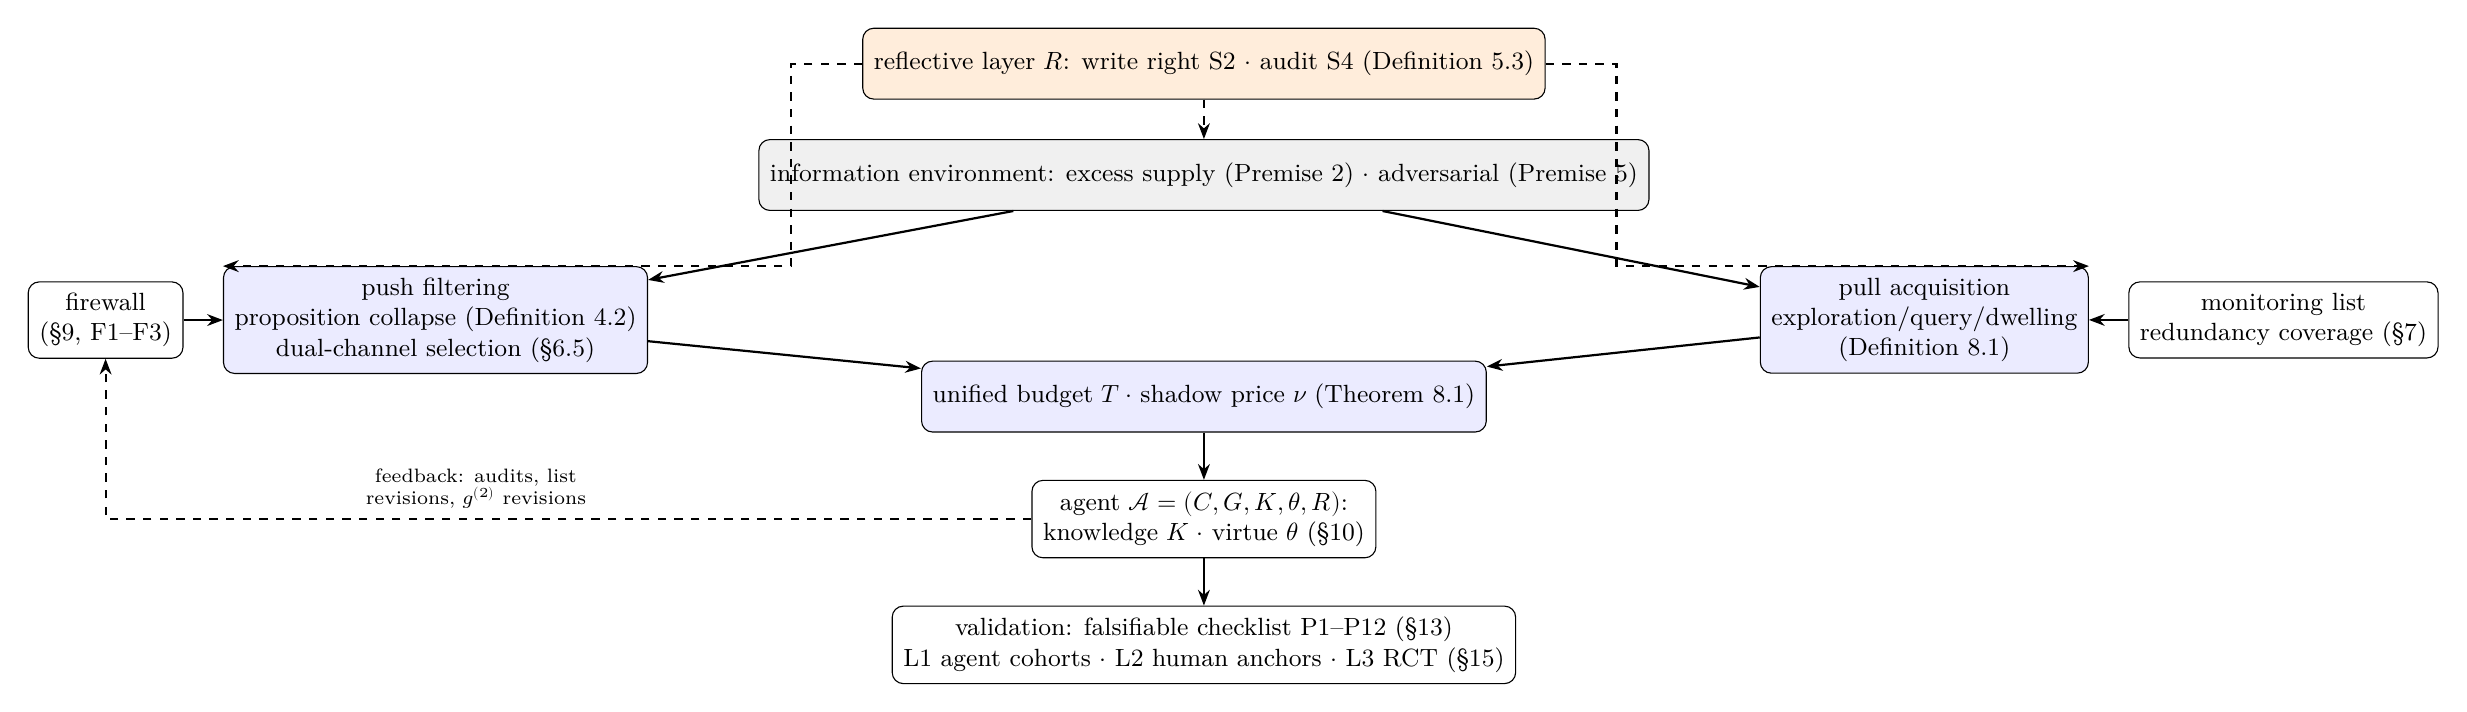
\begin{tikzpicture}[
  font=\small,
  box/.style={draw, rounded corners, align=center, minimum height=0.9cm, inner sep=4pt},
  env/.style={box, fill=gray!12},
  core/.style={box, fill=blue!8},
  rbox/.style={box, fill=orange!14},
  arr/.style={-{Stealth[length=2mm]}, thick},
  node distance=0.5cm and 0.5cm]
\node[rbox] (R) {reflective layer $R$: write right S2 $\cdot$ audit S4 (Definition 5.3)};
\node[env, below=0.5cm of R] (env) {information environment: excess supply (Premise 2) $\cdot$ adversarial (Premise 5)};
\node[core, below left=0.7cm and 1.4cm of env] (push) {push filtering\\ proposition collapse (Definition 4.2)\\ dual-channel selection (\S6.5)};
\node[core, below right=0.7cm and 1.4cm of env] (pull) {pull acquisition\\ exploration/query/dwelling\\ (Definition 8.1)};
\node[box, left=0.5cm of push] (fw) {firewall\\ (\S9, F1--F3)};
\node[box, right=0.5cm of pull] (mon) {monitoring list\\ redundancy coverage (\S7)};
\node[core, below=1.9cm of env] (nu) {unified budget $T$ $\cdot$ shadow price $\nu$ (Theorem 8.1)};
\node[box, below=0.6cm of nu] (agent) {agent $\mathcal{A}=(C,G,K,\theta,R)$:\\ knowledge $K$ $\cdot$ virtue $\theta$ (\S10)};
\node[box, below=0.6cm of agent] (val) {validation: falsifiable checklist P1--P12 (\S13)\\ L1 agent cohorts $\cdot$ L2 human anchors $\cdot$ L3 RCT (\S15)};
\draw[arr] (env) -- (push);
\draw[arr] (env) -- (pull);
\draw[arr] (push) -- (nu);
\draw[arr] (pull) -- (nu);
\draw[arr] (nu) -- (agent);
\draw[arr] (fw) -- (push);
\draw[arr] (mon) -- (pull);
\draw[arr, dashed] (R) -- (env);
\draw[arr, dashed] (R.west) -- ++(-0.9,0) |- (push.north west);
\draw[arr, dashed] (R.east) -- ++(0.9,0) |- (pull.north east);
\draw[arr] (agent) -- (val);
\draw[arr, dashed] (agent.west) -| node[pos=0.3, above, align=center, font=\scriptsize]{feedback: audits, list\\ revisions, $g^{(2)}$ revisions} (fw.south);
\end{tikzpicture}}
\caption{The overall SEA framework: content from the information environment enters unified budget allocation (shadow price $\nu$) via the two operator families of push filtering and pull acquisition; the reflective layer $R$ constrains all writes and audits through S1--S4; the validation layer maps all theorems onto falsifiable propositions.}
\end{figure}

\begin{center}\rule{0.5\linewidth}{0.5pt}\end{center}

\subsection{2 Related Work: Consensus and Controversy across Seven
Disciplinary
Blocks}\label{related-work-consensus-and-controversy-across-seven-disciplinary-blocks}

This section reviews the theoretical foundations along the seven layers
of the problem, marking for each layer the \textbf{consensus} (which may
serve as an engineering premise) and the \textbf{controversy} (which
must be treated as a design variable).

\subsubsection{2.1 Formalizing Scarcity and
Value}\label{formalizing-scarcity-and-value}

\begin{itemize}
\tightlist
\item
  \textbf{Economics of attention} (Simon, 1971): a wealth of information
  creates a poverty of attention. Consensus: the bottleneck lies on the
  attention side.
\item
  \textbf{Bounded rationality and satisficing} (Simon, 1955): under
  computational constraints, agents seek the ``good enough'' rather than
  the optimal. The greedy approximation guarantee of this framework
  (Theorem 6.3) is a normative counterpart of satisficing.
\item
  \textbf{Rational inattention} (Sims, 2003; Maćkowiak, Matějka \&
  Wiederholt, 2023): agents optimally allocate attention subject to
  channel-capacity constraints; the discrete-choice case yields
  softmax-form choice probabilities (Matějka \& McKay, 2015), and
  further analysis of endogenous consideration sets appears in Caplin,
  Dean \& Leahy (2019). A complementary bounded-attention line models
  rationality as \textbf{sparsity}: the agent attends to a
  low-dimensional linear projection of the state and optimally ignores
  the rest (Gabaix, 2014). Strengths: a mature formalization. Weakness:
  the objective function is assumed to be known and stable---yet the
  objective is precisely what the environment reshapes, and this
  literature does not address adversarial content. Section 8.6 of this
  paper connects rational inattention to the SAP as a special case;
  against sparse rationality, SEA's five-dimensional feature map
  \(\phi\) can be read as a \emph{declared and auditable} sparsity
  pattern (S1), in contrast to an optimized-but-implicit attention
  projection. The program continues in macroeconomics with
  information-cost-based attention formation and its general-equilibrium
  consequences (Angeletos \& Sastry, 2025).
\item
  \textbf{Value-of-information theory} (Howard, 1966; Blackwell, 1953;
  Lindley, 1956): the value of information equals the expected
  improvement in decisions, and the informativeness ordering of
  experiments (\(\succeq_B\), Appendix B.5(ii)) is characterized by
  Blackwell's theorem. This literature supports the decomposition in our
  Theorem 5.1; its weakness is its inability to directly price ``being
  informed in general''---this paper supplies the long-term term through
  virtue dynamics (Section 10).
\item
  \textbf{Information foraging theory} (Pirolli \& Card, 1999): agents
  follow information scent, and the decision to stay or to leave obeys
  the marginal value theorem. The theory explains the addictiveness of
  algorithmic feeds, but it is descriptive rather than normative;
  Section 8.3 of this paper elevates it into a normative scheduling
  rule.
\item
  \textbf{The empirical economics of digital addiction and self-control}
  (Allcott et al., 2020; Allcott, Gentzkow \& Song, 2022): social-media
  abstinence experiments provide causal evidence of a systematic
  divergence between first-order preferences and self-reported
  welfare---users retrospectively judge their own consumption to have
  been excessive. This is one of the strongest empirical anchors for
  Premise 3 (the separation of \(g^{(1)}\) from \(g^{(2)}\)), and it
  directly supports the framing of the question ``who owns the objective
  function.''
\end{itemize}

\subsubsection{2.2 Hard Constraints on Cognitive
Processing}\label{hard-constraints-on-cognitive-processing}

Working-memory limits (Miller, 1956; Cowan, 2001---roughly 4 concurrent
units); the selectivity and capacity of attention (Broadbent, 1958);
cognitive load theory (Sweller, 1988); dual-system theory (Kahneman,
2011); the illusory truth effect, whereby repeated exposure by itself
increases perceived truth (Fazio et al., 2015); and the forgetting curve
(Ebbinghaus, 1885). Together, these results constrain the form of the
delivery layer---layered summaries, deduplication, fewer but deeper
items---and support the quantification of Premise 1 (boundedness).

\subsubsection{2.3 Filter Bubbles and Polarization
Mechanisms}\label{filter-bubbles-and-polarization-mechanisms}

\textbf{Consensus}: the evidence on echo chambers---self-organized
homogeneous networks of users---is robust: selective exposure and
homophily are human defaults (Festinger, 1957; McPherson, Smith-Lovin \&
Cook, 2001; Stroud, 2011). The evidence on \textbf{filter bubbles}
(enclosure caused by algorithms alone, Pariser, 2011) is limited and
contested: incidental exposure remains widespread, and the effect of
algorithms alone on polarization is modest (Gentzkow \& Shapiro, 2011;
Guess et al., 2023). \textbf{Epicenter of the controversy}: Bail et
al.~(2018) found that random exposure to opposing views instead
intensified polarization---uncurated ``bubble bursting'' backfires.
Nguyen's (2020) conceptual distinction is crucial for this framework:
epistemic bubbles (a deficit of exposure) are not echo chambers (a
systematic dismantling of trust in outsiders); the latter is the real
problem, and the remedy should therefore shift from ``hearing more
dissent'' to ``choosing and auditing trust anchors.'' This paper
implements that shift as curriculum-based exposure under a
tolerance-radius constraint (Definition 10.2), rather than random
injection. The most recent systematic review of the
filter-bubble/echo-chamber literature consolidates this picture and
stresses that algorithmic curation effects are population- and
platform-dependent (Ahmmad et al., 2025).

\subsubsection{2.4 Manipulation and Immunity (Misinformation
Science)}\label{manipulation-and-immunity-misinformation-science}

\textbf{Consensus}: (a) corrections are on average effective but
incomplete, with a continued-influence effect (Lewandowsky et al., 2012;
Chan et al., 2017; Ecker et al., 2022), and they may fail for
identity-sensitive scientific topics (Chan \& Albarracín,
2023)---\textbf{architectural implication: ex ante filtering as primary,
ex post correction as auxiliary}; (b) lateral reading is the
individually deployable skill with the strongest empirical support
(Wineburg \& McGrew, 2019), and this paper formalizes it as a pull-side
query strategy (Section 8.5); (c) emotional and moralized content
spreads faster and farther, and its spread is driven by humans
(Vosoughi, Roy \& Aral, 2018); (d) identity-protective cognition makes
more cognitively capable individuals more polarized on identity-laden
issues (Kahan, 2017)---being ``smart'' is not immunity, so protection
must be externalized; (e) truth-default theory holds that humans default
to belief and that doubt requires cognitive effort (Levine, 2014)---the
psychological basis on which the goal-capture attack surface exists.

\textbf{Controversy}: inoculation/prebunking effect sizes are small to
moderate and decay over time, with ongoing debate over publication bias
(McGuire, 1964; Roozenbeek \& van der Linden, 2019; van der Linden,
2022); durability is intervention- and follow-up-dependent rather than
uniformly doubtful: Pennycook \& Rand (2022) report no statistically
significant decay over successive trials within an experimental session;
this is not evidence of long-term follow-up durability and must not be
cited as one-directional evidence of decay; and the actual magnitude of
harm from misinformation remains disputed at the level of measurement
(Guess, Nagler \& Tucker, 2019; Grinberg et al., 2019; Allen et al.,
2020; Lazer et al., 2018). The architectural stance of this paper does
not depend on the effect size of any single intervention: \textbf{the
firewall bounds (Theorems 9.1--9.2) take ``measured detector recall ×
bounded per-item impact × exposure cap'' as design parameters}, thereby
converting the effect-size controversy into a parameter-calibration
problem. Two 2025 studies sharpen it: a signal-detection-theory
meta-analysis quantifies inoculation's discrimination gain in \(d'\)
units (Simchon et al., 2025), and five pre-registered simulated-feed
studies---not a field test on a real platform---report limited
feed-level effectiveness of inoculation (Wang et al., 2025)---both
consistent with this paper's stance that intervention effect sizes are
small and that the burden must be carried by architectural defense.

\subsubsection{2.5 The Cognitive Engineering of Human--AI
Collaboration}\label{the-cognitive-engineering-of-humanai-collaboration}

The extended-mind thesis (Clark \& Chalmers, 1998) provides
philosophical legitimacy for human--AI collaboration.
Cognitive-offloading research warns of deskilling risk (Sparrow, Liu \&
Wegner, 2011); our Proposition 10.2 proves the precise location of this
risk within the framework: offloading the judgment-formation process
degrades the calibration measurement channel. Automation bias
(Parasuraman \& Riley, 1997) and algorithm aversion/appreciation
(Dietvorst, Simmons \& Massey, 2015; Logg, Minson \& Moore, 2019)
constrain the design of trust calibration. Goodhart's law (Goodhart,
1984) and value capture (Nguyen, 2019) warn of the necessity of metric
governance; this paper provides constructive protection in the form of
gradient-isolation clauses (Proposition 10.1). Moral crumple zones
(Elish, 2019) warn that human decision must not degenerate into ritual;
this paper implements that requirement through the class-B authenticity
three-condition test (Section 11.1). With the rise of autonomous
LLM-based agents (Xi et al., 2025), the collaboration dyad becomes a
collaboration team, and the security of such agents against injection
and manipulation is itself now a surveyed field (Tang et al.,
2025)---the carrier-level catalogue that our Definition 9.1 abstracts
into a single attack class.

\subsubsection{2.6 Political Economy and
Governance}\label{political-economy-and-governance}

The history of the attention merchants (Wu, 2016), the critique of
surveillance capitalism (Zuboff, 2019), and the claim of a right to
attention (Williams, 2018) correctly identify the incentive-structure
nature of the problem, but their critique outruns their construction.
The structural transformation of the public sphere (Habermas, 1962/1989)
and republican concerns (Sunstein, 2017) point to the public costs of
universal personalization. At the algorithmic level, important empirical
and theoretical work already characterizes these costs: causal
measurement of the effect of feed algorithms on exposure diversity
(Bakshy, Messing \& Adamic, 2015); normative design frameworks for
exposure diversity (Helberger, Karppinen \& D'Acunto, 2018); normative
analysis of ``bubble-bursting'' interventions (Bozdag \& van den Hoven,
2015); and \textbf{algorithmic monoculture} (Kleinberg \& Raghavan,
2021)---when most decision-makers rely on the same algorithm, individual
rationality aggregates into systemic homogenization. The fragmentation
lower bound theorem of Section 12 and the algorithmic-monoculture
literature are two faces of the same problem: the former provides a
constructive guarantee of a ``minimal area of shared reality,'' while
the latter diagnoses the failure mode that arises in the absence of
shared structure. The epistemic-welfare program in communication studies
(Hyzen et al., 2025; Van den Bulck et al., 2025) supplies the
governance-side counterpart: recommender systems are assessed by their
contribution to the epistemic welfare of the public sphere, and
public-service media are proposed as governance anchors---the
institutional analogue of our public agenda layer (Section 12). Finally,
the epistemology of testimony (Coady, 1992; Zagzebski, 2012) supplies
the philosophical foundation: the vast majority of knowledge comes from
the testimony of others, and trust mediation cannot be eliminated---only
chosen and audited. This is the source of Premise 4.

\subsubsection{2.7 The Theoretical Lineage of Active Information
Acquisition}\label{the-theoretical-lineage-of-active-information-acquisition}

The classical tools on the pull side are scattered across six
traditions; Section 8 of this paper brings them into a single framework:

\begin{itemize}
\tightlist
\item
  \textbf{Economics of search} (Stigler, 1961): search is costly, and
  the optimal search depth is determined by the condition marginal
  benefit = marginal cost.
\item
  \textbf{Search with inspection costs / Pandora's box} (Weitzman,
  1979): each ``box'' (candidate source) is costly to open and yields a
  random payoff; the optimal policy opens boxes in descending order of
  the reservation index \(z_i\) (defined by \(E[(X_i - z_i)^+] = c_i\))
  and stops when the best opened value exceeds the remaining indices.
  This is the idealized model of the exploration stage only; actual
  monitoring admission is a separate resource-constrained decision under
  Proposition 8.1(ii), not an iff consequence of a single Pandora
  comparison. Modern extensions of the Pandora model---whether opening
  the box is itself optional (Doval, 2018), and more general stopping
  rules (Olszewski \& Weber, 2015)---share the same structure as the
  problem treated in Section 8 of this paper.
\item
  \textbf{Optimal dynamic information acquisition}: Zhong (2022)
  provides an optimality characterization of the general sequential
  information-acquisition problem (a dynamic version of
  value-of-information indexation) that overlaps almost completely with
  the subject of Section 8. What distinguishes this paper is the
  multi-use joint pricing of the budget (push, pull, and reflection
  sharing a single shadow price) together with the sovereignty
  constraints---not acquisition techniques per se.
\item
  \textbf{Optimal foraging theory} (Charnov, 1976): patch residence time
  is governed by the marginal value theorem---leave when the
  instantaneous intake rate falls to the environmental average (the
  shadow price). The dwelling and rotation of information patches
  thereby acquire normative form (Proposition 8.2); the continual
  scheduling of multiple sources is a restless bandit problem (Gittins,
  1979; Whittle, 1988; Weber \& Weiss, 1990).
\item
  \textbf{Bayesian experimental design and active learning} (DeGroot,
  1962; Lindley, 1956; Chaloner \& Verdinelli, 1995; Settles, 2009):
  DeGroot's (1962) sequential-experiment formulation---choosing each
  experiment to maximize the expected gain in posterior utility---is the
  direct ancestor of this paper's pull-side query planner; the value of
  a query equals the expected information gain (EIG); under
  conditionally independent observations, EIG is monotone and submodular
  in the query set (Krause, Singh \& Guestrin, 2008), and greedy
  selection achieves the \((1-1/e)\) guarantee (Theorem 8.2). Within
  SEA, DeGroot's criterion operates under an attention budget and
  against a declared \(g^{(2)}\), with the Pandora index (Weitzman,
  1979) as its frozen-box special case (§8.6).
\item
  \textbf{Optimal stopping} (Ferguson, 2006): when to stop retrieving
  and switch to consumption is a stopping problem under a budget
  constraint; this paper provides its static characterization via the
  attention no-arbitrage theorem (Theorem 8.1).
\end{itemize}

\textbf{Consensus}: each of these tools is mature, and they are mutually
compatible (all provide opportunity-cost or shadow-price conditions,
with funded-use equalities and corner inequalities made explicit where
applicable). \textbf{Gap}: no tradition simultaneously handles (a)
adversarial content, (b) second-order objectives, (c) joint budget
allocation with push filtering, and (d) long-term virtue dynamics. The
SAP (Definition 5.1) fills precisely this quadruple gap.

\subsubsection{2.8 Cross-Disciplinary Points of
Convergence}\label{cross-disciplinary-points-of-convergence}

The seven disciplines converge on five points, which together form the
premise basis and design principles of this framework:

\begin{enumerate}
\def\labelenumi{\arabic{enumi}.}
\tightlist
\item
  \textbf{Ex ante filtering as primary} (correction effects are limited
  and lagged);
\item
  \textbf{Trust must be chosen and audited} (testimonial mediation
  cannot be eliminated);
\item
  \textbf{Heterogeneous exposure requires curation, not randomization}
  (the backfire evidence);
\item
  \textbf{Humans must retain a genuine judgment load} (the deskilling
  and moral-crumple-zone evidence);
\item
  \textbf{Acquisition and filtering are two faces of the same
  budget-allocation problem, and marginal values must equalize} (the
  common core of the search, foraging, and rational-inattention
  traditions---Theorem 8.1 of this paper elevates it into an organizing
  principle of the framework).
\end{enumerate}

\textbf{Distinction from the closest work (an explicit demarcation of
the new contributions)}. (a) \textbf{Zhong (2022)} provides an
optimality characterization of general sequential information
acquisition and is the theoretical upstream of our pull side; our
differences: the push-filtering channel, the adversarial branch
(negative value under misspecified updating), and the sovereignty
constraints lie outside that framework, and our SAP incorporates them
into a single budget. \textbf{The formal special-case relation (added in
v1.6)}: restrict the SAP by (i) pull channel only
(\(T_{\mathrm{push}} = T_{\mathrm{ref}} = 0\)), (ii) no adversarial
branch (\(c_i \equiv 1\), so \(W\) reduces to VOI and (V5) is vacuous),
(iii) sovereignty constraints inactive (\(\Pi_S = \Pi\)), and (iv)
\(g^{(2)}\) fixed over the horizon (no reflective-layer dynamics). Under
(i)--(iv) the SAP objective reduces to the expected utility gain from a
sequentially chosen information structure under a per-period acquisition
budget---which is the problem class of Zhong (2022), whose dynamic
value-of-information indexation characterizes its optimum. The inclusion
is thus precise: \emph{Zhong (2022) is the special case
SAP\(|_{(i)-(iv)}\)}; the SEA-specific content lies exactly in the
complement---the push channel's per-period selection problem (Sections
6--7), negative-value branches under misspecified updating (Section 9),
and write-access constraints on the objective itself (S1--S4). What this
paper does \textbf{not} claim is any converse reduction (Zhong's
framework cannot express (i)--(iv)'s complements, since its value
objects are nonnegative by construction). (b) \textbf{Weitzman (1979) /
Charnov (1976)} provide the classical rules for exploration admission
and patch leaving; this paper does not re-prove them, but relates them
to the KKT price through the explicit total-utility, slot-to-minute, and
patch-cycle conversions of §8; it does not claim that the Pandora index,
push threshold, Whittle index, and \(\nu\) are numerically identical.
(c) \textbf{KKT / submodular greedy / Hoeffding / Robbins--Siegmund} are
standard tools; our relevant theorems (8.1, 6.3, 9.1--9.2, 10.1) apply
these tools within explicitly restricted structures, with their premises
and open branches defined by v1.8---\textbf{what is new is the structure
and the formulation of the problem} (the sovereignty conditions, the
dual-channel division of labor, human gating), not the tools themselves.
(d) \textbf{Adversarial machine learning} (Dalvi et al., 2004; Lowd \&
Meek, 2005; Biggio \& Roli, 2018) addresses classifier-level
adversaries; our goal-capture model (Definition 9.1) raises the attack
target from classification decisions to the objective function itself,
and write isolation (S2) is a structure absent from that literature (see
§9.1 for details). (e) \textbf{Bounded-confidence opinion dynamics}
(Hegselmann \& Krause, 2002; Deffuant et al., 2000) provides a
ready-made dynamical reference frame for the tolerance-radius curriculum
(Definition 10.2): this paper upgrades the descriptive radius into an
endogenous curriculum that grows with capability. (f) \textbf{Value
learning} (Hadfield-Menell et al., 2016, 2017) addresses alignment under
unknown objectives; our \(g^{(2)}\) declaration plus human gating is an
institutional compromise on the same problem (the guidance note in
§5.3). (g) \textbf{LLM sycophancy} (Sharma et al., 2023) is the most
empirically measured carrier of goal capture on the AI side and is
directly isomorphic to Definition 9.1. (h) \textbf{LLM-agent security
and prompt injection, 2025 surveys} (Geng et al., 2025; Tang et al.,
2025) catalogue carrier-level attacks and defenses for LLM-integrated
applications, including indirect injection through retrieved content;
our Definition 9.1 differs by targeting the \emph{objective function's
write path} rather than any single call's integrity, and by treating
write-right isolation (S2) as a first-class structural defense instead
of an input-sanitization technique---the surveys document the attack
surface, this paper supplies the ownership structure that closes it.

\subsubsection{2.9 Substantive Positioning against the 2025--2026
Adjacent
Literatures}\label{substantive-positioning-against-the-20252026-adjacent-literatures}

The demarcation in §2.8 states where this paper differs; this subsection
states, literature by literature, \textbf{what the adjacent 2025--2026
programs actually assume, what this paper inherits from them, and what
it cannot answer that they can}---the contrasts are substantive rather
than label-level.

\textbf{(a) LLM/RAG information agents and indirect prompt injection (Xi
et al., 2025; Tang et al., 2025; Geng et al., 2025; Liu et al., 2024;
Greshake et al., 2023).} These works treat the agent's failure mode as
\emph{call-integrity}: an injected instruction hijacks one tool call or
one retrieved context, and the defenses are input sanitization,
sandboxing, permission scopes, and detection classifiers. This paper
inherits their attack catalogue (Definition 9.1 abstracts it to a single
carrier-neutral class) and their evidence that retrieval is an attack
surface. The difference is structural, not taxonomic: call-integrity
defenses leave the \emph{objective function's write path} untouched---an
agent whose weights, weights-of-weights, or delivery objective are
silently re-tuned by its operator or by engagement feedback is
compromised without any single call being malformed. S2 (write-right
isolation) is the defense that the injection literature does not possess
because it does not model ownership of the objective; conversely, this
paper inherits from them the honest limitation that S2 is an ownership
structure, not a sanitizer---it cannot stop a payload that persuades the
reflective layer itself (the slow-timescale channel of Proposition
10.1), and their detection rates are precisely the \(\rho_m\) inputs of
our firewall bounds.

\textbf{(b) Recommender welfare, exposure diversity, and
values-in-recommenders (Allcott et al., 2020, 2022; Kleinberg \&
Raghavan, 2021; Kleinberg, Mullainathan \& Raghavan, 2024; Helberger et
al., 2018; Stray et al., 2024; Bozdag \& van den Hoven, 2015).} This
literature optimizes or regulates a \emph{platform-side} objective:
welfare measured by revealed preference, exposure diversity as a design
principle, or values inserted by an interdisciplinary process. It
assumes the objective's owner is the platform (or its regulator) and
asks how to make that objective better or fairer. SEA inherits their
welfare metrics (the S5 baseline of §14.3 uses Allcott et al.'s
revealed-preference welfare as a comparator) and their proof that
engagement optimization is not welfare optimization. The irreducible
difference is \textbf{ownership}: Kleinberg, Mullainathan \& Raghavan
(2024) show that inconsistent preferences make ``what users want''
ill-posed for a platform optimizer; SEA's response is not a better
inference of the user's utility but the relocation of the write right to
the user's reflective layer (S2), converting the ill-posedness into a
declared, revisable \(g^{(2)}\) (the quarterly-revision mechanism of
§5.3). Exposure diversity as a \emph{system-imposed} principle
(Helberger et al.) and the tolerance-radius curriculum as a
\emph{subject-declared} constraint (Definition 10.2) coincide
operationally in many configurations and diverge exactly where the
subject declares a radius narrower than the diversity norm---where this
paper sides with the subject and accepts the paternalism objection as a
residual cost (§16.3, §17 Limitation 5). What this paper cannot answer
that they can: aggregate welfare and marketplace effects of
universalized personalization, which is their object and our externality
(Section 12 only bounds one fragment of it).

\textbf{(c) Information-retrieval recall guarantees and active learning
/ bandit engineering (Settles, 2009; Krause et al., 2008; the IR
evaluation literature).} Engineering practice improves recall by
improving the scorer (better features, better rankers, better retrieval
models); active learning and bandit formulations optimize which labels
or arms to acquire next under a budget. SEA inherits the
submodular-greedy and EIG machinery from this line (Theorems 6.3, 8.2)
and uses measured \(d'\) exactly as this literature uses classifier
quality. The substantive addition is the \emph{impossibility} direction:
Theorem 6.1 prices how much document-level recall a single scalar score
can buy under its stated top-\(m\) and prevalence assumptions at a
99.8\% filtering ratio (the Gaussian specialization gives the
\(d'\approx4.39\) threshold; the measured proxy-dependent range is
0.54--3.49). This gives a model-specific ceiling and motivates a second
structural channel (pass-through, lists, redundancy) as one sufficient
response, not as a requirement on every retrieval architecture. What
this paper cannot answer that they can: within-scorer improvements,
query-planner heuristics, and any guarantee that requires learned
representations---our theorems are representation-agnostic by design,
which is also why they cannot certify a concrete retrieval stack.

\textbf{(d) Public-broadcast and platform governance mechanism design
(Van den Bulck et al., 2025; Hyzen et al., 2025; Helberger et al., 2018;
the public-service-media literature).} These works locate the remedy for
epistemic externalities in institutions: epistemic welfare as a
regulatory objective for public-service media, recommender obligations,
transparency duties. SEA inherits their diagnosis (universal
personalization externalizes a shared-reality cost) and their insistence
that epistemic welfare be operationalized rather than invoked. The
difference is the locus of mechanism design: they design obligations for
providers, SEA designs a \emph{personal} sovereignty layer plus a
minimal public floor (Section 12) and proves only a fragmentation lower
bound for that floor. The two are complements, not competitors: the
public layer's \(\gamma\) and attestation classes are exactly the
parameters a regulator could mandate as a floor beneath personal
sovereignty, and our certification-reversal negative result (market-only
lift 0.615→1.230; market∪legal lift 0.626→1.359) is a warning addressed
to their design space---raw-count attestation is gameable by attention
inflation (O7). What this paper cannot answer that they can: the
political-economy feasibility of any mandate, and the distributional
questions of who bears the cost of the floor.

\textbf{Net position}. In each of the four literatures the 2025--2026
frontier moves by better models, better metrics, or better institutions;
\textbf{this paper does not claim to surpass any of them on models,
metrics, or institutional design}. Its only claim is that one variable
they all take as given---the \textbf{ownership of the acquisition
objective}---is itself a design variable with a formal structure
(S1--S4), and that fixing it changes which guarantees are attainable
(the dual-channel necessity of Theorem 6.1, the write-isolation defense
absent from the injection literature, the declared-radius substitute for
imposed diversity). The novelty claim is therefore exactly as stated in
§2.8(c): new structure and problem formulation, standard tools.

\begin{center}\rule{0.5\linewidth}{0.5pt}\end{center}

\section{Part II Premises and Formal
Framework}\label{part-ii-premises-and-formal-framework}

\subsection{3 Working Hypotheses and Design
Principles}\label{working-hypotheses-and-design-principles}

\subsubsection{3.1 Six Premises: Empirical Assumptions, Normative
Assumptions, and Design
Stances}\label{six-premises-empirical-assumptions-normative-assumptions-and-design-stances}

This framework rests on six premises. \textbf{To forestall any
misleading connotation of the word ``premise,'' we state explicitly at
the outset}: these are not mathematical premises---claims that could
enter derivations as unexamined givens---but claims of three distinct
epistemic statuses: \textbf{empirical assumptions} (measurable and
falsifiable: Premises 1, 2, 4), \textbf{normative assumptions}
(philosophical positions and value stipulations: Premise 3), and
\textbf{design stances} (engineering and governance commitments:
Premises 5, 6). Each premise is labeled with its category and its
\textbf{testability}, and each explicitly shoulders the corresponding
empirical risk or argumentative burden. The theorems below depend only
on the empirical assumptions; the normative assumptions and design
stances determine how the problem is formulated and how the institution
is designed, and they never enter the logical premise chain of any proof
(wherever they do enter, this is declared through separately and
explicitly numbered conditional assumptions R/F/C/P, etc.).

\textbf{Premise 1 (Boundedness)}. {[}Empirical assumption{]} The
information-processing capacity of every agent is bounded: there exist a
per-period cognitive budget \(T < \infty\) (time and attention) and a
working-memory constraint \(W\) (for humans, \(W \approx 4\) concurrent
units, Cowan, 2001; for AI agents, the context window and inference
budget). Quantitative basis: Section 2.2.

\textbf{Premise 2 (Excess Supply)}. {[}Empirical assumption (including
an order-of-magnitude extrapolation){]} The candidate-supply rate
\(\lambda\) (items/day) of the information environment and the per-item
consumption cost \(\bar t\) satisfy \(\lambda \bar t \gg T\), and under
the generative-AI regime the growth of \(\lambda\) is no longer
constrained by production costs. Current order of magnitude:
\(\lambda \bar t / T \approx 10^3\) (recomputed from the typical
parameters of §1.1---\(T=45\), \(\bar t\approx4\), \(N\sim10^4\)---as
\(8.9\times10^2\)). Testability: supply volume and costs are directly
measurable, and that ``production cost tends to zero'' is an industrial
fact. \textbf{Corollary}: a filtering ratio of
\(1 - T/(\lambda \bar t) \ge 99.8\%\) is an arithmetic necessity
(Proposition 6.1).

\textbf{Premise 3 (Goal Stratification)}. {[}Normative assumption
(philosophical foundation: Frankfurt, 1971){]} The agent's goal
structure \(G = (g^{(1)}, g^{(2)})\) is stratified: \(g^{(1)}\)
comprises first-order preferences (the impulse at the moment of
clicking, the immediate pull of high-arousal content), whereas
\(g^{(2)}\) is the second-order will---the goals, endorsed by the
reflective layer \(R\), concerning ``what one wishes to be shaped by.''
The two can diverge systematically; \textbf{normatively, \(g^{(2)}\)
holds authority over the shaping of the information environment}.
Empirical support: the planner--doer structure of self-control (Thaler
\& Shefrin, 1981), intertemporal inconsistency (Ainslie, 1992), and the
endogenous shaping of preferences (Elster, 1983).

\textbf{Premise 4 (Testimonial Dependence)}. {[}Empirical assumption
(epistemological foundation: Coady, 1992; Zagzebski, 2012){]} The
overwhelming majority of an agent's beliefs about the world are acquired
through the testimony of others; trust mediation cannot be
eliminated---it can only be \textbf{chosen} (through the source
portfolio) and \textbf{audited} (through provenance and calibration).
Corollary: the provenance structure (Definition 4.2) is not optional
metadata but a load-bearing wall of belief formation.

\textbf{Premise 5 (Adversariality)}. {[}Design stance (worst-case
assumption){]} The information environment contains actors whose payoffs
depend on rewriting the goals or beliefs within the agent's processing
loop, and whose strategies adapt to defenses (an arms race). This is
formalized in Definition 9.1 (the goal-capture attack). Human instances:
emotional hijacking and the propaganda ``firehose of falsehood'' (Paul
\& Matthews, 2016); AI instances: prompt injection, especially indirect
prompt injection delivered through retrieved content (Greshake et al.,
2023; Liu et al., 2024). \textbf{A filtering theory that does not posit
this premise does not hold in open environments.}

\textbf{Premise 6 (Measurability \& Correctability)}. {[}Design
stance{]} Filter performance (recall, precision, manipulation exposure)
and the agent's cognitive state \(\theta\) can be measured, albeit
noisily, and correction channels (parameter rollback, source
replacement, goal revision) are always open. This is the
governance-theoretic converse of Goodhart's law: a filter that cannot be
measured cannot be governed.

\subsubsection{3.2 The Invariants and Their
Derivation}\label{the-invariants-and-their-derivation}

\textbf{Proposition 3.1 (Invariants I1--I5; argued derivation)}.
\emph{Under Premises 1--6, any sovereign epistemic acquisition system
must satisfy the following invariants.} (This proposition belongs to the
``Proposition (argued)'' tier: I1 admits a rigorous derivation; I2--I5
are conceptual derivations from premises to design requirements, whose
function is to make the operational implications of the premises
explicit rather than to serve as mathematical theorems.)

\begin{itemize}
\tightlist
\item
  \textbf{I1 (Capacity constraint)}: \(C \ll |X|\); filtering and
  prioritization are unavoidable; the only open question is who owns the
  acquisition--filtering mechanism and what objective function it
  serves.
\item
  \textbf{I2 (Sovereignty)}: the write right over the objective function
  \(g^{(2)}\) and the filter parameters \(w\) resides with the subject's
  reflective layer \(R\) (or its legitimate delegate).
\item
  \textbf{I3 (Provenance)}: every accepted proposition carries
  verifiable provenance. Human instances: primary sources (papers,
  financial reports, court judgments, raw data); machine instances:
  cryptographically signed origins and content credentials (C2PA, 2021).
\item
  \textbf{I4 (Adversarial robustness)}: there exists a bound
  \(\varepsilon\) such that, after the processing of any adversarial
  content sequence, the effective-goal divergence satisfies
  \(D(\tilde U, G) \le \varepsilon\) (Section 9 gives the exact metric
  \(D\) and the construction of the bound).
\item
  \textbf{I5 (Calibration)}: filter performance is measurable and
  auditable, and the correction channel is open.
\end{itemize}

\textbf{Proof.}

\emph{I1}: By Premise 1, the consumption budget \(T\) is finite; by
Premise 2, \(\lambda \bar t > T\). Hence any policy consumes at most
\(m \le T/\bar t < \lambda\) items per day, and the discarded fraction
is \(\ge 1 - T/(\lambda\bar t) > 0\) and approaches 1. Filtering---in
the broad sense of selective admission into the candidate pool---occurs
under every policy, so the only remaining question is ``by whom, and
according to what objective.'' \(\blacksquare\)

\emph{I2}: By Premise 3, \(g^{(1)}\) and \(g^{(2)}\) are separable, with
normative authority residing in \(g^{(2)}\). The filter's objective
function determines which content enters the agent's belief-formation
loop, and thereby \textbf{shapes the future \(g^{(1)}\) and even
\(g^{(2)}\) itself} (preference endogeneity, Elster, 1983). If the write
right does not belong to \(R\), the mechanism amounts to a third party's
enforced execution upon the subject's goal structure; by the procedural
definition of autonomy (the Frankfurt hierarchy condition plus the
procedural-independence condition), this is not the subject's autonomous
acquisition but heteronomous shaping. Sovereignty therefore requires
that the write right \(\in R\). \(\blacksquare\)

\textbf{Remark (adaptive preferences and the limits of the procedural
criterion---added in v1.6)}. The I2 argument relies on a
\emph{procedural} reading of the Frankfurt hierarchy condition:
endorsement by the reflective layer \(R\) confers authority on
\(g^{(2)}\). The classic objection (Elster, 1983---sour grapes) is that
\(g^{(2)}\) itself may be shaped by an impoverished information
environment, so that ``reflective endorsement'' may ratify
\emph{adapted} preferences rather than autonomous ones. This paper does
not claim to dissolve that objection---no tool can (§16.6 concedes the
point). What the framework adds is structural: (i) the input set from
which endorsement is formed is kept non-degenerate \textbf{by default}
(the tolerance-radius curriculum and the public layer are both on by
default, opt-out with logging under S4); (ii) the shaping channel is
made \textbf{auditable} (write isolation S2 + tamper-proof logs S4), so
an adapted \(g^{(2)}\) is at least traceable to its formation history;
(iii) revision remains possible at every governance cycle (§16.4). The
sovereignty claimed here is therefore precisely ``procedural autonomy
\textbf{plus auditable, default-non-degenerate formation
conditions}''---not a substantive guarantee that \(g^{(2)}\) is
authentically the subject's own, which is a philosophical problem
outside the scope of any engineering framework.

\emph{I3}: By Premise 4, beliefs are mediated by testimony, and the
reliability of that mediation cannot be assumed a priori (Premise 5:
there exist adversaries who forge the mediation). Verifiable provenance
is the only way to convert ``trust'' from an unauditable psychological
state into an auditable structural property: without provenance there is
no object to audit, and I5 fails; and if provenance can be forged
without cryptographic or institutional anchoring, then the adversary of
Premise 5 can inject false testimony. I3 is thus a conjunctive corollary
of I5 together with Premises 4--5. \(\blacksquare\)

\emph{I4}: Premise 5 asserts that adversaries exist and adapt. If the
goal divergence were unbounded, the system's effective objective
function could be rewritten by content, and I2 would exist in name
only---the write right would be stolen through the content channel,
bypassing the authorized path. I4 is therefore the preservation
condition for I2 in adversarial environments; the construction of
\(\varepsilon\) is given in Theorems 9.1--9.2. \(\blacksquare\)

\emph{I5}: Given directly by Premise 6. Note the logical hierarchy:
Premise 6 is itself a design stance rather than an empirical fact, so I5
is a \textbf{design requirement} (``the system ought to be built this
way''), not an empirical invariant; its empirical component (``whether
measurement is feasible'') is borne by the measurement model of Section
10.1 and by the measurements of Sections 14--15. A supplementary
argument: if performance were not measurable, then (a) the correction
channel could never be triggered, (b) Goodhart drift could never be
detected, and (c) the audit right (S4) of I2 would spin idle.
\(\blacksquare\)

\subsubsection{3.3 The Human--AI Symmetry
Table}\label{the-humanai-symmetry-table}

The invariants and all subsequent mechanisms instantiate symmetrically
across the two classes of agents; this is the operational meaning of the
claim that ``the methodology applies to every bounded agent'':

\begin{longtable}[]{@{}
  >{\raggedright\arraybackslash}p{(\linewidth - 4\tabcolsep) * \real{0.3333}}
  >{\raggedright\arraybackslash}p{(\linewidth - 4\tabcolsep) * \real{0.3333}}
  >{\raggedright\arraybackslash}p{(\linewidth - 4\tabcolsep) * \real{0.3333}}@{}}
\toprule\noalign{}
\begin{minipage}[b]{\linewidth}\raggedright
Structure
\end{minipage} & \begin{minipage}[b]{\linewidth}\raggedright
Human instantiation
\end{minipage} & \begin{minipage}[b]{\linewidth}\raggedright
AI-agent instantiation
\end{minipage} \\
\midrule\noalign{}
\endhead
\bottomrule\noalign{}
\endlastfoot
Capacity constraint (Premise 1) & working memory, time budget & context
window, inference budget \\
Goal stratification (Premise 3) & impulses vs.~reflectively endorsed
goals & immediate instruction-following vs.~the principal's authorized
configuration \\
Adversarial capture (Premise 5) & emotional hijacking (System 1 arousal
hijacking the weights) & prompt injection (instructions rewritten by
content) \\
Provenance (I3) & primary-source verification & signed origins, content
credentials \\
Reflective layer \(R\) & the person themself & the legitimate
authorization configuration of the principal \\
Virtue state \(\theta\) & calibration, openness, humility & calibration,
robustness (no humility dimension; replaced by an overconfidence penalty
term) \\
pull operator & active retrieval, subscription trial and error & tool
calls, sub-queries, retrieval augmentation \\
push operator & feed filtering & admission control over the input
queue \\
\end{longtable}

\subsection{4 The Information Environment and the Agent
Model}\label{the-information-environment-and-the-agent-model}

This section fixes all of the mathematical objects. The
measure-theoretic setup is minimal but rigorous: all random elements are
defined on a common filtered probability space
\((\Omega, \mathcal{F}, \{\mathcal{F}_t\}_{t\ge0}, P)\), and ``a.s.''
always means \(P\)-almost surely.

\subsubsection{4.1 Information Items and the Arrival
Process}\label{information-items-and-the-arrival-process}

\textbf{Definition 4.1 (Information item)}. The information flow
\(X = \{x_1, x_2, \dots\}\) is a marked point process over arrival times
\(\{t_i^{arr}\}\) (for the push stream we take compound Poisson arrivals
at rate \(\lambda\); for modeling extensions, see the simulations in
Section 14). Each item
\[x_i = (\mathrm{content}_i,\ \mathrm{prov}_i,\ \tau_i),\] where
\(\mathrm{prov}_i\) is the provenance information (source identity,
signatures/credentials, the chain of paraphrase) and \(\tau_i > 0\) is
the consumption-time cost. Each item carries latent attributes
(unobservable, or only noisily observable, to the filter):

\begin{itemize}
\tightlist
\item
  \(v_i^* \in \mathbb{R}\): \textbf{true realized decision value}---the
  ground truth of the strength of association between the proposition to
  which the item belongs and the subject's decision set (defined
  precisely via the VOI decomposition of Theorem 5.1);
\item
  \(m_i \in [0,1]\): \textbf{manipulation intensity}---the strength of
  the goal-capture payload embedded in the content (Definition 9.1);
\item
  \(s_i \in \mathcal{S}\): \textbf{stance vector}---a position on the
  issue-relevant stance manifold \(\mathcal{S}\).
\end{itemize}

The observable feature map is \(\phi(x_i;\, K, D) \in [0,1]^5\),
\(\phi = (\text{relevance}, \text{novelty}, \text{durability}, \text{actionability}, \text{credibility})_i\).
\textbf{A note on the type signature}: \(\phi\) is a function of
\textbf{item × subject state}, not of the item alone---relevance depends
on the subject's declared decision set \(D\), and novelty depends on the
knowledge state \(K\) (there is no gain on information already contained
in \(K\)). This point is substantive: any formulation that treats
\(\phi\) as a pure item function \(X \to [0,1]^5\) is inconsistent with
the decomposition of Theorem 5.1. Theorem 5.1 gives the
decision-by-decision structural decomposition of \(v_i^*\) and proves
that, under decision homogeneity (V4) together with benefit-side
representability (V4a) and harm homogeneity or explicit harm
representability (V4b), \(\phi(\cdot; K, D)\) is an exact summary of
\(v_i^*\) (there exists an \(F\) such that \(v_i^* = F(\phi)\)); outside
(V4), \(\phi\) is only an engineering heuristic summary (§5.2 gives an
explicit counterexample).

\textbf{Definition 4.2 (Proposition graph and provenance tree)}. Let
\(E = \{e_j\}\) be the underlying set of events/propositions. Generative
structure: each proposition \(e_j\) derives a document set
\(D_j \subseteq X\), and the collapsing map \(\kappa: X \to E\) sends
each document to its proposition. Each proposition carries a
\textbf{provenance tree} \(T_j\): the root node is the primary source,
with verification status
\(r(T_j) \in \{\mathrm{verified}, \mathrm{unverified}\}\); the branch
nodes are paraphrases and commentary. \textbf{Commentary is not
independent information but an annotation layer on the
proposition}---its value enters as a bounded correction term to the
proposition's value and does not separately consume a full share of the
consumption budget.

\textbf{Definition 4.3 (Proposition-collapse ratio)}.
\(\rho_c := |X| / |E|\). The proposition-centric architecture makes
repostings collapse automatically: \(n\) media outlets reposting = 1
proposition + \(n\) provenance-tree edges. Prior prediction:
\(\rho_c \in [5, 20]\) (tested in simulation and on real measurements,
Section 13, P3). \textbf{Corollary 6.1 shows} that collapse converts the
document-level filtering-ratio problem into a proposition-level
selection problem. It is one sufficient way to relax the stated
document-capacity bottleneck, not a necessary feature of every
architecture; it also changes the recall unit, so document-level and
proposition-level recall must be reported separately.

\textbf{Definition 4.4 (Source classes)}. The universe of sources is
partitioned by the triple (ownership × geography × type) into
\textbf{source classes} \(\mathcal{C}_1, \dots, \mathcal{C}_K\). The
purpose of the partition is to approximate the conditional independence
of coverage events (Assumption R2): outlets under the same ownership or
upstream of the same wire service are assigned to the same class,
whereby cross-class correlation is constructively suppressed. The
\textbf{coverage event} of class \(i\) for proposition \(e\) is
\(Z_i(e) := \mathbb{1}\{\exists x \in D_e: \text{the source of } x \in \mathcal{C}_i\}\).

\subsubsection{4.2 The Agent}\label{the-agent}

\textbf{Definition 4.5 (The agent five-tuple)}.
\[\mathcal{A} = (C,\ G,\ K,\ \theta,\ R)\]

\begin{itemize}
\tightlist
\item
  \(C = (T, W)\): cognitive capacity---the per-period budget \(T\)
  (minutes) and the working-memory constraint \(W\);
\item
  \(G = (g^{(1)}, g^{(2)})\): the goal structure (Premise 3);
\item
  \(K\): \textbf{knowledge state}---a belief measure
  \(\mu_K \in \mathcal{P}(\Theta_{\mathrm{rel}})\) over the state space
  \(\Theta_{\mathrm{rel}}\) relevant to the subject's decision set,
  together with a memory of the set of consumed propositions (used in
  the novelty computation: the novelty of item \(i\)
  \(= I(y_i; \omega \mid K)\), see Section 8.5);
\item
  \(\theta = (\theta_{\mathrm{cal}}, \theta_{\mathrm{open}}, \theta_{\mathrm{hum}}) \in [0,1]^3\):
  the cognitive-virtue state (Section 10 gives the measurement model and
  the dynamics);
\item
  \(R\): the reflective layer---for a human, the person themself; for an
  AI agent, the legitimate authorization configuration of its principal.
\end{itemize}

\textbf{Definition 4.6 (Decision set)}. \(D\) is the subject's declared
\textbf{active decision set} (finite): each \(d \in D\) carries a
decision deadline \(h_d\) (horizon) and a utility function
\(u_d(a, \omega)\). Criticality is defined on this basis: a proposition
\(e\) is \textbf{critical} for the subject (\(e \in E^*\)) if there
exists \(d \in D\) such that information about \(e\) has a nonzero
probability of changing the optimal action of \(d\), with the magnitude
of the change exceeding a declared threshold. \textbf{Criticality is
subject-relative}---this paper makes this explicit, and it is precisely
what renders the recall target arithmetically feasible (the
budget-feasibility condition of Proposition 6.3).

\subsubsection{4.3 Acquisition--Filtering
Policies}\label{acquisitionfiltering-policies}

\textbf{Definition 4.7 (The policy five-tuple)}. A policy is
\(\pi = (\pi_{\mathrm{mon}}, \pi_{\mathrm{pull}}, \pi_{\mathrm{push}}, \pi_{\mathrm{del}}, \pi_{\mathrm{esc}})\):

\begin{itemize}
\tightlist
\item
  \(\pi_{\mathrm{mon}}\): \textbf{monitoring list}---the subset of
  source classes admitted for direct pass-through and the watchlist of
  monitored entities (Assumption R3); a slow variable (updated
  weekly/monthly), subject to slow-timescale gating (§10.3, Assumption
  C5-H);
\item
  \(\pi_{\mathrm{pull}}\): \textbf{active-acquisition policy}---query
  generation, retrieval depth, source exploration, patch dwelling and
  rotation (Section 8);
\item
  \(\pi_{\mathrm{push}}\): \textbf{filtering policy}---the selection
  \(A \subseteq X\) from the candidate pool (push arrivals ∪ pull
  returns) (Section 6);
\item
  \(\pi_{\mathrm{del}}\): \textbf{delivery policy}---layered summaries,
  ranking, cooling-queue scheduling; it obeys the ``summary = map''
  principle (the class-C constraints of Section 11.1);
\item
  \(\pi_{\mathrm{esc}}\): \textbf{emergency-override
  policy}---conservative actions under pre-authorization instructions
  (Section 11).
\end{itemize}

\textbf{Budget identity}:
\(T = T_{\mathrm{pull}} + T_{\mathrm{push}} + T_{\mathrm{ref}}\), where
\(T_{\mathrm{ref}}\) is the reflection load (the weekly calibration
meeting, etc.; class C, not automatable). Theorem 8.1 gives the
optimality condition for this partition.

\subsubsection{4.4 The Producer Ecology}\label{the-producer-ecology}

\textbf{Definition 4.8 (Producer game environment)}. The population of
content producers is distributed across types
\(q \in \{\mathrm{honest}, \mathrm{sensational}, \mathrm{manipulative}\}\),
with share vector \(\mathbf{x} = (x_h, x_s, x_m)\), \(\sum_i x_i = 1\).
Producers choose content strategies to maximize payoffs \(\Pi(q)\)
(Section 9.4 gives the payoff structure); shares evolve under replicator
dynamics. The adoption rate \(\sigma \in [0,1]\) of the filter (the
fraction of sovereign-filter users in the population) is an exogenous
parameter of producer payoffs; the endogenization of \(\sigma\) (users
adopting according to the quality of the ecology) is left as an open
problem (Section 17).

\begin{center}\rule{0.5\linewidth}{0.5pt}\end{center}

\subsection{5 The Sovereign Acquisition Problem (SAP) and the
Value-of-Information Decomposition
Theorem}\label{the-sovereign-acquisition-problem-sap-and-the-value-of-information-decomposition-theorem}

\subsubsection{5.1 The Sovereign Acquisition
Problem}\label{the-sovereign-acquisition-problem}

\textbf{Definition 5.1 (Sovereign Acquisition Problem, SAP)}. Given a
horizon \(H\) (number of periods) and a discount factor
\(\beta \in (0,1]\), the SAP is:

\[\max_{\pi \in \Pi_S}\ \mathbb{E}_\pi\!\left[\sum_{t=1}^{H} \beta^t \Big( \underbrace{\mathrm{VOI}_t(A_t)}_{\text{current-period information value}} + \underbrace{\zeta\, \Delta\theta_t}_{\text{virtue gain}} - \underbrace{\mathrm{Harm}_t(A_t)}_{\text{manipulation harm}} \Big)\right]\]

subject to:

\begin{itemize}
\tightlist
\item
  \textbf{(Budget)} in each period,
  \(\sum_{i \in A_t} \tau_i + c(\pi_{\mathrm{pull},t}) + c_{\mathrm{ref}} \le T\),
  where \(c(\pi_{\mathrm{pull},t})\) is the time cost of active
  acquisition (queries, exploration, reading retrieval results) and
  \(c_{\mathrm{ref}}\) is the incompressible reflection load;
\item
  \textbf{(Manipulation exposure)}
  \(\mathbb{E}[\#\{i \in A_t: m_i > \tau_m\}] \le \varepsilon_c / (\delta(1-\rho_m))\)
  (obtained by inverting the bound
  \(D \le \delta(1-\rho_m)\,\mathbb{E}[n_m] \le \varepsilon_c\) of
  Theorem 9.1);
\item
  \textbf{(Tolerance band)} the stance dispersion of the exposure set
  satisfies \(d(E_t) \le \rho(\theta_t)\) (Definition 10.2, the
  no-backfire constraint);
\item
  \textbf{(Sovereignty constraints)} \(\pi \in \Pi_S\): the policy space
  is restricted by S1--S4 (Definition 5.3)---the objective function is
  readable, parameter writes must be authorized by \(R\), there are no
  third-party revenue terms, and decisions are auditable;
\item
  \textbf{(Emergency structure)} \(\pi_{\mathrm{esc}}\) is restricted to
  the class of pre-authorization instructions (Definition 11.2).
\end{itemize}

\textbf{Remark (dimensional consistency)}. In the objective functional,
\(\mathrm{VOI}_t\) and \(\mathrm{Harm}_t\) are both measured in the same
decision-utility unit (for the definition of \(\mathrm{Harm}\) see §5.2:
the expected utility loss under misspecified updating), so the two are
additive; \(\zeta\,\Delta\theta_t\) is a slow-timescale term, and
\(\zeta\) is the subject's declared ``virtue--utility exchange rate'' (a
class-B decision)---its very existence is the operationalization of
Premise 3: the subject explicitly declares the weight of long-term
virtue relative to current-period information value. The shadow price
\(\nu\) of ``VOI/minute'' in Section 8 unifies the units across push,
pull, and reflection precisely because the value functions of all three
uses are expressed as functions of time in the same utility unit.

The SAP is a stochastic control problem: the exploration--exploitation
trade-off on the pull side, online selection on the push side, and the
slow-timescale \(\theta\) dynamics and monitoring-list updates are all
coupled together. \textbf{This paper does not solve the full SAP to
global optimality} (the general case contains restless-bandit special
cases that are already PSPACE-hard, Papadimitriou \& Tsitsiklis, 1999;
see §8.6 for the complexity discussion); instead, it adopts a strategy
of ``decomposition + layer-by-layer optimality guarantees'': Section 6
solves the push-selection layer (submodular greedy + threshold
policies), Section 7 solves the coverage guarantee of the monitoring
list, Section 8 solves the pull layer and gives the no-arbitrage
condition for budget allocation among the three layers (Theorem 8.1),
and Sections 9--12 equip the layers with the safety, sublimation,
emergency, and publicness constraints. \textbf{An honest statement}:
layer-by-layer optimality does not automatically compose into global
approximate optimality---the layers are coupled through the shared
budget and the knowledge state, and this paper has not proved a general
theorem to the effect that per-layer approximation ratios multiply or
that errors propagate linearly; what this paper provides is an explicit
characterization of each layer's error terms (the distortion lower
bound, the coverage miss bound, the firewall bounds, the
convergence-neighborhood bound) and of the channels through which they
enter the SAP objective; under the weak-coupling conditions (W1)--(W4)
the remark in §8.8 gives an additive composed bound, and the rigorous
propagation bound for the general coupling case is listed as open
problem O8. The simulations (Section 14) test the actual performance of
the decomposition strategy on end-to-end KPIs.

\textbf{Proposition 5.1 (Existence of an optimal policy)}. \emph{Suppose
the horizon \(H\) is finite, per-period rewards are bounded
(\(|\mathrm{VOI}_t|, |\mathrm{Harm}_t| \le \bar V < \infty\)), the
per-period candidate pool is finite (so that the per-period action
set---the Cartesian product of the family of candidate-pool subsets with
the finite combinations of pull operators---is finite), and the
constraint sets (budget, exposure, tolerance band, sovereignty
constraints S1--S4, emergency structure) are closed period by period.
Then the SAP admits an optimal (deterministic Markov) policy, not
necessarily unique.}

\textbf{Proof (finite-horizon dynamic programming)}. Under the standard
hypotheses of finite per-period action sets, bounded rewards, and finite
horizon, backward induction for the finite-horizon MDP applies directly:
define the terminal value function \(V_{H+1}(\cdot) \equiv 0\) and
recurse from \(t = H\) down to \(t = 1\) via
\[V_t(s_t) = \max_{a_t \in \mathcal{A}_t(s_t)}\ \Big\{ r_t(s_t, a_t) + \beta\,\mathbb{E}\big[V_{t+1}(s_{t+1}) \mid s_t, a_t\big] \Big\},\]
where
\(s_t = (K_t, \theta_t, \text{remaining budget}, \pi_{\mathrm{mon},t})\)
is a sufficient state and \(\mathcal{A}_t(s_t)\) is the current feasible
action set (nonempty: the null-consumption action is always feasible).
Since each \(\mathcal{A}_t\) is finite, the maximum is attained and an
optimal action rule exists in every period; inductive concatenation then
yields a globally optimal policy. The role of the sovereignty
constraints S1--S4 is to shrink each period's \(\mathcal{A}_t\)
(removing policies with unauthorized parameter writes or third-party
revenue terms); this shrinking does not alter per-period finiteness, so
the existence conclusion is unaffected. \textbf{A clarification on the
proof's technical level (added in v1.6)}: under the standing finiteness
assumptions (finite horizon, finite per-period action set), \textbf{no
measurable-selection machinery is actually required}---a maximum over a
finite set is attained by inspection, and the backward induction above
is self-contained. The measurable-selection theory of Bertsekas \&
Shreve (1978) is cited not because the finite argument needs it, but to
mark the standard route by which the same existence result extends to
Borel state spaces (the belief \(\mu_K\) is a probability measure)
should the finiteness assumptions ever be relaxed: the selection
machinery of their Chapter 7 (``Borel Spaces and their Probability
Measures,'' in particular the universally measurable selection results)
together with the Borel-model existence results of their Chapters 8--9
(``The Finite Horizon Borel Model'' and ``The Infinite Horizon Borel
Models''; chapter numbers vary across printings, the chapter titles are
the stable identifiers). The citation is a generalization marker, not a
load-bearing step. \(\blacksquare\)

\textbf{Remark (on the choice of proof route)}. This paper does not take
the route of ``weak compactness of the policy space + maximizing a
continuous functional'': weak compactness of the space of conditional
transition kernels requires the relaxed-control (Young measure)
framework, and the authorization constraint of S2 confines parameters to
the set approved by \(R\)---a set that is generally not closed and hence
incompatible with compactness arguments. The DP route is both more
elementary and more rigorous under this paper's own assumptions (finite
horizon, per-period finite actions, bounded rewards).

\subsubsection{5.2 The Feature Decomposition of Information
Value}\label{the-feature-decomposition-of-information-value}

The scoring function is the core of the entire engineering design. This
section provides decision-theoretic foundations for the five-dimensional
feature vector: under explicit assumptions, it derives a
decision-by-decision structural decomposition of an item's
\textbf{expected realized decision value}, and it characterizes
precisely the additional conditions under which ``the five-dimensional
feature is a summary of it'' holds ((V4) plus (V4a) and (V4b), together
with counterexamples showing failure). The section also honestly
addresses a conceptual difficulty: within the Blackwell framework, the
value of information of any experiment is nonnegative (Lemma 5.1),
whereas adversarial content can obviously inflict negative value;
reconciling the two requires an explicit ``misspecified updating''
modeling step (Definition 5.2), which constitutes the main technical
content of this section.

\textbf{Setup}. State space \(\Theta_{\mathrm{rel}}\) (the world states
relevant to the decision set \(D\)); the subject's current belief
\(\mu_K\). The generation of an item \(x_i\) is a \textbf{two-branch
mixture}: with probability \(c_i\) (the source's credibility) it is the
true branch, in which the item provides a genuine signal \(y_i\) about
\(\Theta_{\mathrm{rel}}\) (information structure \(\sigma_i\)); with
probability \(1 - c_i\) it is the false branch, in which the item
carries a signal \(\tilde y_i\) chosen by the adversary (aimed at
pushing beliefs in a direction favorable to the adversary). When
consuming the item, the subject \textbf{cannot observe the branch
label}---this is precisely the substance of the adversarial problem.

\textbf{Lemma 5.1 (The EVPI identity and nonnegativity)}. \emph{For any
regular decision problem satisfying Appendix B.5(i)'s attainment and
integrability conditions (in particular, a finite action set, or more
generally existence of the required maxima, with integrable displayed
expectations), and any experiment \(\sigma\) for which those
expectations exist, when the subject performs Bayesian updating with the
correct likelihood:}
\[\mathrm{VOI}(\sigma) := \mathbb{E}_{y \sim \sigma}\Big[\max_a \mathbb{E}[u(a,\omega) \mid y]\Big] - \max_a \mathbb{E}[u(a,\omega)] \ \ge\ 0.\]

\emph{For the proof see Appendix B.5} (a one-line corollary of Jensen's
inequality; Blackwell (1953) further characterizes the informativeness
ordering among experiments).

\textbf{Corollary-like observation (why the adversarial branch is not a
Blackwell experiment)}. The nonnegativity of Lemma 5.1 presupposes that
the subject updates with the \textbf{correct likelihood}. The harm
mechanism of adversarial content lies precisely in the fact that the
subject \textbf{updates with a misspecified likelihood}---treating the
adversarial signal \(\tilde y\) as if it were the genuine signal \(y\).
The ``value'' of the adversarial branch is therefore not the VOI of any
Blackwell experiment and must be defined separately.

\textbf{Definition 5.2 (Expected realized decision value under
misspecified updating)}. For a decision \(d\) and a signal \(z\) (with
true distribution \(Q_z\)), suppose the subject updates the belief to
the posterior \(\mu_K^{\ell}(\cdot \mid z)\) according to a (possibly
misspecified) likelihood \(\ell\), and accordingly chooses the action
\(\hat a(z) = \arg\max_a \mathbb{E}_{\mu_K^{\ell}(\cdot\mid z)}[u_d(a,\omega)]\).
Assume the same regularity as Lemma 5.1 for the baseline and for every
posterior used: the required maxima are attained and all displayed
expectations are integrable (finite action sets provide one sufficient
attainment condition). Define the \textbf{expected realized decision
value}
\[W_d(z;\ \ell) := \mathbb{E}_{z \sim Q_z}\,\mathbb{E}_{\omega \sim P(\cdot \mid z)}\big[u_d(\hat a(z), \omega)\big] - \max_a \mathbb{E}_{\mu_K}[u_d(a,\omega)],\]
where the outer expectation is taken under the \textbf{true} joint
distribution. Under updating with the correct likelihood,
\(W_d(z;\ell_{\mathrm{true}}) = \mathrm{VOI}_d(z) \ge 0\) (Lemma 5.1);
under updating with a misspecified likelihood, \(W_d\) can be strictly
negative (the posterior is systematically pushed away from the truth,
and the action is worse than remaining at \(a_0\)).

\textbf{Assumptions} (the feature-decomposition assumptions (V1)--(V5)):

\begin{itemize}
\tightlist
\item
  \textbf{(V1) Decision relevance}: an item affects the subject's
  utility only through the decisions in \(D\):
  \(v_i^* = \sum_{d \in D} P(d \text{ active within the horizon and } i \text{ relevant to it}) \cdot W_i^{(d)}\),
  where \(W_i^{(d)}\) is the item's expected realized decision value for
  decision \(d\). Being informed in general is not priced through \(D\);
  its value enters the slow-timescale virtue term \(\zeta \Delta\theta\)
  (Section 10)---this honestly acknowledges that the decision-theoretic
  framework cannot price ``cultivation''; cultivation is handled
  separately by the cybernetics of sublimation.
\item
  \textbf{(V2) Branch mixture with bounded harm}: in the true branch the
  subject updates with the correct likelihood, and the realized value is
  the Blackwell value of information
  \(W_i^{(d)}(y_i;\ell_{\mathrm{true}}) = \mathrm{VOI}_i^{(d)}(y_i) \ge 0\);
  in the false branch the subject updates with the misspecified
  likelihood ``the signal is genuine,'' and the realized value satisfies
  \(W_i^{(d)}(\tilde y_i;\ell_{\mathrm{mis}}) \le 0\) and is bounded
  below: define the \textbf{harm term}
  \(\mathrm{Harm}_i^{(d)} := -W_i^{(d)}(\tilde y_i;\ell_{\mathrm{mis}}) \in [0, \mathrm{Harm}_{\max}]\)
  (the boundedness of single-item harm and the bounded-per-item-impact
  assumption F1 of Section 9 are two faces of the same coin).
\item
  \textbf{(V3) Timeliness discounting}: the information value of
  decision \(d\) is discounted by \(e^{-h/\lambda_d}\) as a function of
  the time gap \(h\) between the arrival of the information and the
  decision deadline (\(\lambda_d\) is the decision's \textbf{durability
  scale}: for one-off event news \(\lambda_d\) is small; for
  foundational knowledge \(\lambda_d\) is large).
\item
  \textbf{(V4) Decision homogeneity} (the additional assumption required
  for an exact summary): all decisions \(d \in D\) share the same
  durability scale \(\lambda_d = \lambda\), and the per-decision values
  decompose along a common profile:
  \(\mathrm{VOI}_i^{(d)}(y_i) = a_d \cdot V_i\),
  \(\mathrm{Harm}_i^{(d)} = a_d \cdot H_i\), where \(a_d \ge 0\) is the
  importance weight of decision \(d\) (independent of the item), and
  \(V_i, H_i\) are the item's decision-independent value and harm
  baselines. The substance of (V4): decisions differ only in ``weight,''
  not in value structure.
\item
  \textbf{(V4a) Benefit-side representability for the five-dimensional
  summary}: there exist known calibrated maps
  \(\mathcal A,\mathcal V,\mathcal D_\lambda,\mathcal C\) such that, for
  every item, \(A_i=\mathcal A(\phi_i)\), \(V_i=\mathcal V(\phi_i)\),
  \(e^{-h_i/\lambda}=\mathcal D_\lambda(\phi_i)\), and
  \(c_i=\mathcal C(\phi_i)\). These identities are formal
  representability assumptions, not consequences of naming the
  coordinates relevance, novelty, durability, actionability, and
  credibility. In particular, equal conditional mutual information
  \(I(y_i;\omega\mid K)\) does not by itself imply equal Blackwell VOI;
  novelty can be used only after such a calibrated map has been
  validated.
\item
  \textbf{(V4b) Harm homogeneity or representability for the
  five-dimensional summary}: either \(H_i=H\) for every item for a
  calibrated constant \(H\), or a known calibrated map \(\mathcal H\) is
  explicitly assumed such that \(H_i=\mathcal H(\phi(x_i;K,D))\) for
  every item. Merely saying that harm is ``folded into the features''
  does not establish this condition. If \(H_i\) varies with \(i\) and no
  such map is given, the decomposition remains valid but the original
  five-dimensional vector is not an exact summary; the augmented
  representation \((\phi,H_i)\) is required.
\item
  \textbf{(V5) Branch--update consistency} (added in v1.6 as an explicit
  assumption; previously implicit in (V2) and the remark below): the
  data-generating branch indicator corresponds to the updating rule the
  subject actually applies. In the true branch, the subject updates
  under the correctly specified likelihood, and the realized value
  equals the Blackwell value of information
  \(\mathrm{VOI}_i^{(d)}(y_i)\); in the false branch, the subject
  updates under the misspecified likelihood ``the signal is genuine,''
  and the realized value equals \(-\mathrm{Harm}_i^{(d)}\). Consequently
  the composite quantity \(W_i^{(d)}\) (Definition 5.2) is \textbf{not}
  the Blackwell value of any single experiment: the two branches arise
  from \emph{different updating rules} (correctly specified
  vs.~misspecified likelihood), not from a posterior mixture within one
  experiment. (V5) is the structural assumption that licenses reading
  the branch expectation in Theorem 5.1 as an application of the law of
  total expectation over the branch indicator.
\end{itemize}

\textbf{Theorem 5.1 (Feature decomposition of the expected realized
decision value)}. \emph{Under (V1)--(V3) and the branch--update
consistency convention (V5), the expected realized decision value of
item \(x_i\) for the subject decomposes as}

\[v_i^* \;=\; \sum_{d \in D} \pi_d(i)\,\Big[\, c_i\,\mathrm{VOI}_i^{(d)}(y_i)\,e^{-h_i/\lambda_d} \;-\; (1 - c_i)\,\mathrm{Harm}_i^{(d)} \,\Big]\]

\emph{Reading of the factors (the semantic annotations are stated here
in prose, deliberately kept out of the display so that no annotation can
be misread as a denominator):}
\(\pi_d(i) = P(d \text{ active and relevant} \mid i)\) \emph{is the
relevance--actionability weight; \(c_i\,\mathrm{VOI}_i^{(d)}(y_i)\) is
the credibility-weighted novelty factor, where
\(\mathrm{VOI}_i^{(d)}(y_i) \ge 0\) (Lemma 5.1) is the Blackwell value
of information and is monotone nondecreasing in the informativeness
ordering of experiments (Blackwell, 1953); \(e^{-h_i/\lambda_d}\) is the
durability (timeliness) discount of (V3), multiplying the true-branch
value only; and \((1-c_i)\,\mathrm{Harm}_i^{(d)}\), with
\(\mathrm{Harm}_i^{(d)} \in [0, \mathrm{Harm}_{\max}]\), is the
adversarial-branch penalty. The above is a \textbf{decision-by-decision
(\(d\)-dependent) structural decomposition}: it expresses \(v_i^*\) as a
combination of calibratable components, but the right-hand side in
general \textbf{cannot} be reconstructed from any finite-dimensional
scalar feature of the item (see the counterexample in the remark below).
\textbf{Aggregation under (V4)}: substituting
\(\mathrm{VOI}_i^{(d)} = a_d V_i\), \(\mathrm{Harm}_i^{(d)} = a_d H_i\),
\(\lambda_d = \lambda\) and factoring \(a_d\) out of the bracket
collapses the display to
\(v_i^* = A_i[c_iV_ie^{-h_i/\lambda} - (1-c_i)H_i]\) with
\(A_i := \sum_d \pi_d(i)a_d\)---an item-dependent expression for which
the exact five-dimensional summary requires both (V4a) and (V4b).
\textbf{Exact-summary conclusion (sufficient conditions)}: under (V4),
(V4a), and (V4b), define \(A_i := \sum_d \pi_d(i)\,a_d\) (relevance ×
actionability), and use the calibrated maps
\(\mathcal A,\mathcal V,\mathcal D_\lambda,\mathcal C,\mathcal H\);
then}
\[v_i^*=\mathcal A(\phi_i)\Big[\mathcal C(\phi_i)\mathcal V(\phi_i)\mathcal D_\lambda(\phi_i)-(1-\mathcal C(\phi_i))\mathcal H(\phi_i)\Big]=:F_{\lambda,\mathcal A,\mathcal V,\mathcal D_\lambda,\mathcal C,\mathcal H}(\phi_i).\]
\emph{Thus we prove exactness under the \textbf{sufficient} conditions
(V4), (V4a), and (V4b); these are not asserted to be necessary. Under
(V4) alone, the valid conclusion is only the exact augmented
representation \(v_i^*=F_\lambda(A_i,V_i,h_i,c_i,H_i)\). If the
benefit-side maps fail, the augmented vector \((A_i,V_i,h_i,c_i,H_i)\)
is required; if only harm representability fails, \((\phi,H_i)\) is
required. Two items with identical raw feature readings can have
different net values whenever these maps are not assumed. Without the
stated representability assumptions, exactness does not follow and the
five-dimensional feature is an engineering heuristic summary.}

\textbf{Proof}. Step 1 (decomposition): by (V1),
\(v_i^* = \sum_d \pi_d(i)\,W_i^{(d)}\). Step 2 (branch mixture): the
item's value is an expectation taken over the \textbf{data-generating
branches}---with probability \(c_i\) it falls in the true branch (value
\(\mathrm{VOI}_i^{(d)}(y_i)\)), and with probability \(1-c_i\) it falls
in the false branch (value \(-\mathrm{Harm}_i^{(d)}\), by (V2) and
Definition 5.2). The expectation is linear in the branch indicator (this
is merely taking the expectation of a discrete random variable), so
\[W_i^{(d)} = c_i\,\mathrm{VOI}_i^{(d)}(y_i) - (1-c_i)\,\mathrm{Harm}_i^{(d)}.\]
Step 3 (timeliness): by (V3), the true-branch value is multiplied by the
discount \(e^{-h_i/\lambda_d}\) (the harm of the false branch is
realized in the period of consumption and receives no timeliness
discount---this asymmetry reflects that ``bad information distorts
judgment immediately, whereas the value of good information depends on
decision timing''). Combining the three steps yields the decomposition.
Summariness: the right-hand side of the decomposition depends on \(i\)
only through \((\pi_d(i))_{d}\), \(\mathrm{VOI}_i^{(d)}(y_i)\),
\(h_i/\lambda_d\), and \(c_i\); \(\pi_d(i)\) is ``relevance ×
actionability''; \(\mathrm{VOI}_i^{(d)}(y_i)\) is a decision-specific
value of information, not a monotone function of conditional mutual
information: Blackwell's informativeness order does not imply such a
scalar representation. Conditional mutual information
\(I(y_i;\omega\mid K)\) may serve as an engineering novelty proxy only
after a separate calibration to the relevant decision value has been
validated (as required by V4a); \(h_i, \lambda_d\) are ``durability'';
and \(c_i\) is ``credibility.'' The exact-summary part: under (V4),
substituting \(\mathrm{VOI}_i^{(d)} = a_dV_i\),
\(\mathrm{Harm}_i^{(d)} = a_dH_i\), and \(\lambda_d = \lambda\), and
factoring \(a_d\) out of the summand, gives
\(v_i^* = \big(\sum_d \pi_d(i)a_d\big)\big[c_iV_ie^{-h_i/\lambda} - (1-c_i)H_i\big]\),
whose right-hand side still contains \(H_i\) explicitly. Under (V4a),
all benefit-side quantities are known functions of \(\phi_i\); under
(V4b), either \(H_i=H\) or \(H_i=\mathcal H(\phi_i)\). Hence the
right-hand side depends on \(i\) only through \(\phi_i\) with fixed
calibrated \(\lambda\) and maps, completing the sufficient-condition
exactness proof. Without (V4a) or (V4b), the same argument yields only
the augmented representation \((A_i,V_i,h_i,c_i,H_i)\). (Note: without
(V4) this step fails---\(\sum_d \pi_d(i)\,[\,\cdot\,]_d\) is a sum of
products of \(d\)-dependent quantities and in general is not a function
of any low-dimensional aggregate.) \(\blacksquare\)

\textbf{Remark (the exact status of this theorem---answering two
misreadings)}.

\begin{enumerate}
\def\labelenumi{\arabic{enumi}.}
\tightlist
\item
  \textbf{Why Step 2 is not a ``linear decomposition of VOI over
  posterior mixtures''}: if the item were modeled as a single Blackwell
  experiment (the posterior mixing as
  \(\mu_{K\oplus x_i} = c_i\mu_{K\oplus y_i} + (1-c_i)\mu_{K\oplus\tilde y_i}\)),
  then the nonlinearity of the \(\max_a\) operator would make the VOI of
  the mixed experiment \textbf{generally unequal} to the linear mixture
  of the VOIs, and by Lemma 5.1 that VOI would have to be
  nonnegative---one would neither obtain the decomposition nor
  accommodate the harm term. The decomposition of this paper takes
  expectations not at the posterior level but at the level of the
  \textbf{data-generating branches}: the branch indicator is part of the
  real world (whether the content is or is not an adversarial payload),
  taking expectations over it is an ordinary application of the law of
  total expectation, and linearity holds trivially. The price is that
  \(W\) (Definition 5.2) replaces VOI as the value concept---it is not
  the Blackwell value of any single experiment, but ``the expected
  realized utility change of an agent acting on its own updating rule
  under a class of generative processes.'' \textbf{This is now the
  explicit content of assumption (V5)}: the correspondence between the
  branch indicator and the subject's actual updating rule is an
  assumption of the theorem, not a consequence of the Blackwell
  framework, and readers should not mistake the decomposition for a
  standard within-Blackwell result.
\item
  \textbf{Status in the general case}: the decomposition relies on the
  structure of (V1)--(V3); \textbf{the exact-summary conclusion
  additionally relies on (V4), (V4a), and (V4b)}. Without any of these
  sufficient conditions (interacting decisions, non-exponential
  timeliness, within-branch updating rules adaptive to content,
  heterogeneous value structures across decisions), the five-dimensional
  feature vector should be regarded as an \textbf{engineering heuristic
  summary} rather than a sufficient statistic for value; under the
  Gaussian--quadratic structure plus (V4), (V4a), and (V4b) it is exact
  (Corollary 5.1). Accordingly, the decision-theoretic foundation of
  this paper's scoring function is a ``conditional summary theorem under
  structural assumptions,'' not an unconditional identity.
  Independently, even when (V4) holds, two items can share all five
  feature coordinates while \(H_i\ne H_j\); if \(A>0\) and \(c<1\),
  their net values differ by \(-A(1-c)(H_i-H_j)\), which directly
  refutes five-dimensional summariness without (V4b).
\item
  \textbf{Counterexample (when representability fails)}: let
  \(D=\{d_1,d_2\}\) have different durability scales
  \(\lambda_1\ne\lambda_2\). Item \(i\) is relevant only to \(d_1\) and
  item \(j\) only to \(d_2\). A heuristic scorer may assign them the
  same raw semantic feature readings while no common calibrated
  \(\mathcal D_\lambda\) exists; then \(v_i^*\propto e^{-h/\lambda_1}\)
  and \(v_j^*\propto e^{-h/\lambda_2}\), so the raw readings do not
  determine net value. If, by contrast, (V4a) is imposed and
  \(\mathcal D_\lambda(\phi)\) is an exact coordinate map, identical
  \(\phi\) would force identical effective discounts and this example
  would not be a counterexample. The failure is therefore lack of
  representability, not an ambiguity that can be resolved by naming a
  coordinate ``durability.''
\item
  \textbf{The status of linear scoring \(\langle w, \phi\rangle\)}: the
  engineering objective of the SAP and Definition 9.1 use linear
  scoring, whereas the exact \(F\) under (V4) is multiplicative/bilinear
  (\(A \cdot [cVe^{-h/\lambda} - (1-c)H]\)). The two are reconciled as
  follows: (a) the complete pure-benefit term is
  \(B_i:=A_ic_iV_ie^{-h_i/\lambda}\) with \(A_i\ge0\). Whenever
  \(A_i>0\), \(c_i>0\), and \(V_i>0\),
  \(\log B_i=\log A_i+\log c_i+\log V_i-h_i/\lambda\) is additive in
  \((\log A_i,\log c_i,\log V_i,h_i)\). Linear scoring on these
  log-features is therefore \textbf{order-equivalent} to \(B_i\), not
  numerically identical to it; \(A_i\) may be omitted only if it is a
  positive item-independent constant. If \(A_ic_iV_i=0\), either handle
  the zero-benefit case separately or adopt the extended convention
  \(\log B_i=-\infty\), under which all zero-benefit items tie; (b) the
  harm term \(-(1-c)H\) cannot be added to the benefit term in the same
  log space, and this paper's treatment is \textbf{architectural
  separation}: the harm channel is borne by the firewall (Section 9,
  with hard constraints on \(\rho_m, n_{\max}\)) rather than by the
  scoring function, and scoring is responsible only for benefit-side
  ranking; (c) outside this structure, no approximation bound between
  \(\langle w, \phi\rangle\) and \(F\) has been proved, and linear
  scoring is an engineering heuristic---this paper no longer claims any
  unconditional decision-theoretic justification for it; its ranking
  quality is priced by the measured \(d'\) (the usage in Theorem 6.1 is
  precisely ``do not assume the scores are correct; price the scoring
  error'').
\end{enumerate}

\textbf{Corollary 5.1 (Gaussian--quadratic closed form)}. \emph{If for
every critical decision \(d\): \(\omega_d \in \mathbb{R}\), with prior
\(\omega_d \sim \mathcal{N}(\hat\omega, \sigma_0^2)\), signal
\(y_i = \omega_d + \epsilon_i\) with
\(\epsilon_i \sim \mathcal{N}(0, \sigma_i^2)\) \textbf{independent of
\(\omega_d\)}, \(\sigma_0^2+\sigma_i^2>0\), and quadratic utility
\(u_d(a,\omega_d) = -(a - \omega_d)^2\), then}
\[\mathrm{VOI}_i^{(d)}(y_i) \;=\; \sigma_0^2 - \frac{\sigma_0^2 \sigma_i^2}{\sigma_0^2 + \sigma_i^2} \;=\; \frac{\sigma_0^4}{\sigma_0^2 + \sigma_i^2} \;=\; \sigma_0^2 \cdot \frac{\sigma_0^2}{\sigma_0^2 + \sigma_i^2}.\]
\emph{That is, information value = prior variance × (the share of
posterior-precision gain). The ``novelty'' dimension of the scoring
function is, under this closed form, an estimate of the precision gain
\(\sigma_0^2/(\sigma_0^2+\sigma_i^2)\), and ``relevance'' is
\(\pi_d(i)\). Here \(\sigma_i^2\) is an independent within-true-branch
signal-noise parameter, whereas \(c_i=P(\text{true branch})\) is a
branch probability. No map from \(c_i\) to \(\sigma_i^2\) is implied;
any such calibration, including representability through the
five-dimensional features, must be separately assumed and validated.}

\textbf{Proof}. Under quadratic utility,
\(\max_a \mathbb{E}[u] = -\mathrm{Var}\), so
\(\mathrm{VOI} = \mathrm{Var}(\text{prior}) - \mathbb{E}[\mathrm{Var}(\text{posterior})] = \sigma_0^2 - \frac{\sigma_0^2\sigma_i^2}{\sigma_0^2+\sigma_i^2} = \frac{\sigma_0^4}{\sigma_0^2 + \sigma_i^2}\).
Rearranging gives the result (the final expression
\(= \sigma_0^2 \cdot \frac{\sigma_0^2}{\sigma_0^2+\sigma_i^2}\)).
\(\blacksquare\)

\textbf{Engineering implications}. (a) On decision structures where
(V4), (V4a), and (V4b) hold, the scoring weights \(w\) are not free
parameters: the dimensions of \(w\) are images of the decision weights
\(\pi_d a_d\), the durability scale \(\lambda\) (the actual decay factor
being \(e^{-h_i/\lambda}\)), and the harm bound \(\mathrm{Harm}_{\max}\)
in \(F\)---what S2 (the write right) constrains is therefore \textbf{the
decision set and the utility declarations}, not arbitrary numbers;
outside (V4), the calibration of \(w\) can only proceed empirically
(measured \(d'\) and retrospective audits) and enjoys no structural
derivation; (b) the novelty dimension may use conditional mutual
information \(I(y_i; \omega \mid K)\) as an engineering proxy, but only
after separately calibrating it to decision-specific VOI; neither
Blackwell's order nor mutual information alone supplies the V4a
representability map (Section 8.5 gives a computable submodular
information measure, not a universal value calibration); (c) \textbf{if
a net-value score is used}, the \(\mathrm{Harm}\) term correctly pushes
high-relevance, low-credibility items to negative scores. Under the
benefit-only architecture adopted in remark 4 above, harm is instead
handled exclusively by the firewall; these are alternative scoring
conventions, not one undifferentiated implementation. In both cases,
firewall recall \(\rho_m\) lowers the arrival rate of the false branch
and hence the expected \((1-c_i)\mathrm{Harm}\) contribution.

\subsubsection{5.3 Sovereignty Conditions and the Reversibility
Principle}\label{sovereignty-conditions-and-the-reversibility-principle}

\textbf{Definition 5.3 (Sovereignty conditions S1--S4)}. An
acquisition--filtering system \((\pi, U)\) is \textbf{sovereign} if and
only if:

\begin{itemize}
\tightlist
\item
  \textbf{S1 (Inspectability)}: the objective functional \(U\) is
  represented in an interpretable form of at most \(k\) terms (in this
  paper \(k = 5\): the five dimensions of \(\phi\)), and the weights
  \(w\) and \(g^{(2)}\) are fully readable by the reflective layer
  \(R\);
\item
  \textbf{S2 (Write right)}: any modification to \(w\), \(g^{(2)}\),
  threshold parameters, or the monitoring list \(\pi_{\mathrm{mon}}\)
  must be explicitly authorized by \(R\) via \(\sigma_R\); the system
  must not use behavioral data to implicitly rewrite the objective
  function (click signals may be used only for \textbf{measurement},
  never for \textbf{writing}---the line separating this framework from
  platform recommender systems lies here);
\item
  \textbf{S3 (Non-capturability)}: \(U\) contains no term related to any
  third party's revenue. Idealized statement:
  \(I(U;\ \mathrm{Rev}_{\mathrm{platform}}) = 0\) (mutual information is
  zero). Operationalized audit: code review + provenance logs of weights
  + ranking counterfactual tests (for the same content pool, verifying
  that the ranking does not change with platform-side variables);
\item
  \textbf{S4 (Auditability)}: every delivery carries an explanation
  \(e(i) =\) the top-\(j\) contributing features together with their
  signs; all ranking and admission decisions leave tamper-proof logs.
\end{itemize}

\textbf{Definition 5.4 (Reversibility principle)}. Every parameter
modification takes effect immediately, is historically traceable, and
can be rolled back in one click. The system must not lock the subject in
through sunk costs, migration barriers, or default inertia.
Formalization: the switching-cost function on the policy-parameter space
satisfies \(c_{\mathrm{switch}}(\cdot,\cdot) \equiv 0\) (borne by the
system, not passed on to the subject).

\textbf{Remark (the relationship between the S-conditions and the SAP)}.
S1--S4 do not enter the SAP's objective functional; they shrink its
policy space \(\Pi_S\): sovereignty is a constraint, not a preference
term. The rationale for this design: if sovereignty could be traded away
for utility, then in a world where \(g^{(1)}\) is shaped by the
environment it inevitably would be traded away (Premise 3 + Elster's
sour-grapes mechanism). The sovereignty conditions are the system-level
form of a Ulysses contract (Section 11).

\textbf{Remark (the elicitation burden of \(g^{(2)}\)---the largest
usability gap of this framework)}. The SAP and S2 require the subject to
declare the decision set \(D\), utilities \(u_d\), horizons \(h_d\), the
tolerance threshold \(\varepsilon_c\), and the pre-authorization
specification \(D_{\mathrm{adv}}\)---\textbf{an ordinary subject cannot
write down their own utility function}; this is the elicitation
difficulty shared by all value-alignment research, and this paper is no
exception. The literature lines most relevant to this problem:
cooperative inverse reinforcement learning (CIRL, in which
Hadfield-Menell et al.~(2016) formalize ``the subject's goals are
unknown and must be learned through interaction'' as a two-player
cooperative game) and the Off-Switch Game (correctability as an
equilibrium property of a game, Hadfield-Menell et al., 2017). This
paper's position is an engineering compromise rather than a solution:
(a) the declaration burden is \textbf{tiered by explicitness}---the
minimal viable declaration consists of only two items, the monitoring
list and the weekly time budget, with all utility parameters set to
conservative defaults (defaults as a governance problem of values: see
§16.2); (b) \(g^{(2)}\), as a slow variable, is iteratively refined
through quarterly goal-revision meetings (class C, Proposition 10.2)
rather than elicited once and for all---this is spiritually isomorphic
to CIRL's ``learning goals through interaction,'' but with human gating
replacing automated preference inference (avoiding the consolidation of
inference errors into writes); (c) measurable proxies for elicitation
quality: the convergence over time of declaration-revision magnitudes
(declaration stabilization) and the ``declaration--behavior'' gap (the
deviation between the declared \(E^*\) and the topics actually
consumed). \textbf{On well-definedness under iterative elicitation
(added in v1.6)}: there is no circularity in declaring \(g^{(2)}\) while
acknowledging that it may need interaction to discover---the SAP
objective is defined \textbf{relative to the declaration in force at the
current decision epoch}, and revision of \(g^{(2)}\) is itself a
governed act (class-C decision, human-gated, logged under S4); each
epoch's optimization problem is therefore well-defined given the current
declaration. What must be conceded is a \textbf{snapshot approximation}:
if the subject's ``true'' \(g^{(2)}\) is only discoverable through
interaction (the CIRL picture), each epoch optimizes against the best
current declaration rather than against a fixed latent objective. The
framework's convergence claims are stated correspondingly weakly and
explicitly---convergence to the \emph{declared} neighborhood (Theorem
10.1 / Conjecture 10.1), with declaration quality itself monitored
through the proxies in (c). A complete formalization (a CIRL-ized SEA)
is left to future work (see the extension of Limitation 12 in §17).

\begin{center}\rule{0.5\linewidth}{0.5pt}\end{center}

\section{Part III Core Theorems}\label{part-iii-core-theorems}

\subsection{6 An Efficiency Theory of Passive Filtering
(Push)}\label{an-efficiency-theory-of-passive-filtering-push}

This section answers the second of the four questions: ``On what grounds
is filtering safe?'' The answer unfolds in four layers. The capacity and
distortion lower bounds (6.1) quantify what aggressive filtering costs;
the score-separability bottleneck theorem (6.2) characterizes when the
stated single-score document-level top-\(m\) model cannot support high
recall, thereby motivating---but not proving universally necessary---the
dual-channel architecture (proposition collapse + source-redundancy
direct pass-through + scored discovery); submodularity and
restricted-domain greedy guarantees (6.3) yield near-optimal selection
only under the conditions stated there; threshold policies (6.4)
characterize the optimal structure of the online case; and 6.5
synthesizes all of these results into the dual-channel architecture
principle.

\subsubsection{6.1 Capacity and Distortion Lower
Bounds}\label{capacity-and-distortion-lower-bounds}

\textbf{Proposition 6.1 (Arithmetic lower bound of the filtering
ratio)}. \emph{Suppose \(N\) candidates arrive per period, with per-item
consumption cost \(\tau_i \ge \underline\tau > 0\) and budget \(T\).
Then any policy consumes \(m \le T/\underline\tau\) items per period,
and the discarded fraction is}
\[1 - \frac{m}{N} \ \ge\ 1 - \frac{T}{\underline\tau N}.\]
\emph{Substituting typical values---\(T = 45\) minutes,
\(\underline\tau \approx 4\) minutes/item (deep-reading one substantive
item), \(N = 10^4\)---yields a filtering ratio \(\ge 99.8\%\).}

\textbf{Proof}. Consumption is constrained by the budget:
\(m\underline\tau \le \sum_{i\in A}\tau_i \le T\). \(\blacksquare\)

\textbf{Definition 6.1 (Critical-value leakage / distortion)}. For a
policy \(\pi\), define the distortion
\[\mathcal{D}(\pi) := \mathbb{E}\Big[\sum_{e \in E^*} v_e \cdot \mathbb{1}\{e \text{ not consumed}\}\Big],\]
that is, the expected sum of the true values of the uncovered part of
the critical-proposition set \(E^*\) (Definition 4.6). This is the exact
measure of ``the cost of aggressive filtering.''

\textbf{Proposition 6.2 (The distortion lower bound and optimal
distortion)}. \emph{Let \(K^* = |E^*|\) be the number of critical
propositions in the current period, with values \(\{v_e\}\), and suppose
the consumption budget accommodates \(m\) distinct propositions. Then,
for any policy,}
\[\mathcal{D}(\pi) \ \ge\ \mathcal{D}^* := \mathbb{E}\Big[\sum_{r > m} V_{(r)}\Big],\]
\emph{where \(V_{(1)} \ge V_{(2)} \ge \dots\) is the decreasing
rearrangement of \(\{v_e\}\). Equality holds if and only if the policy
consumes exactly the top-\(m\) critical propositions by value (perfect
ranking, with the entire budget directed at critical propositions).}

\emph{If, in addition,
\(v_e \stackrel{iid}{\sim} \mathrm{Pareto}(\alpha, v_{\min})\)
(\(\alpha > 1\), power-law criticality---the setting of the simulation
generator), then}
\[\frac{\mathcal{D}^*}{\mathbb{E}[\sum_e v_e]} \ =\ 1 - \Big(\frac{m}{K^*}\Big)^{(\alpha-1)/\alpha}.\]

\textbf{Proof}. First claim: any policy consumes at most \(m\) distinct
propositions, so the leaked value = total critical value − consumed
critical value \(\ge\) total critical value − the \(m\) largest critical
values \(= \sum_{r>m} V_{(r)}\); a perfectly ranking policy attains
equality. Second claim: the Pareto tail is
\(P(V > v) = (v/v_{\min})^{-\alpha}\), with quantile function
\(Q(1-u) = v_{\min} u^{-1/\alpha}\). The expected total is
\(\mathbb{E}[\sum_e v_e] = K^* v_{\min} \alpha/(\alpha - 1)\). The
expected sum of the top \(m\) terms is approximated by an integral over
order statistics:
\[\mathbb{E}\Big[\sum_{r \le m} V_{(r)}\Big] \approx K^* v_{\min} \int_0^{m/K^*} u^{-1/\alpha}\, du = K^* v_{\min} \frac{\alpha}{\alpha-1}\Big(\frac{m}{K^*}\Big)^{(\alpha-1)/\alpha}.\]
Subtracting and dividing by the total gives the result. \(\blacksquare\)

\textbf{Remark (accuracy of the approximation)}. The integral
approximation above has relative error \(o(1)\) as \(m \to \infty\)
(with \(m/K^*\) bounded or tending to zero) (Resnick, 1987); for small
\(m\) the exact order statistics carry \(\Gamma\) correction factors
(\(\mathbb{E}[V_{(r)}] = v_{\min}\frac{\Gamma(r-1/\alpha)\Gamma(K^*+1)}{\Gamma(r)\Gamma(K^*+1-1/\alpha)}\),
which for small \(r\) differ from \(v_{\min}(K^*/r)^{1/\alpha}\) by a
factor of order \(\Gamma(1-1/\alpha)\); at \(\alpha=1.5\) the first-term
deviation can reach double-digit percentages). This paper's typical
usage range \(m/K^* \in [0.5, 0.8]\) does not lie entirely in the
asymptotic regime, so the closed form should be read as a
\textbf{first-order approximation}, and the numbers derived from it
(such as 20.6\% and 7.2\% below) carry correspondingly generous
tolerances; the simulation (P2) tests directly against the generator's
exact order statistics. \textbf{Explicit error bounds for the two
printed numbers (added in v1.6)}: evaluating the aggregate leaked share
\(\sum_{r>m}\mathbb{E}[V_{(r)}]\big/\sum_{r}\mathbb{E}[V_{(r)}]\)
exactly through the \(\Gamma\) formula displayed above (a deterministic
computation, reproducible from that formula alone) gives, at the pilot
scale \(K^*=52\) and \(\alpha=1.5\): \textbf{20.8\%} at \(m/K^*=0.5\)
(\(m=26\)) and \textbf{6.9\%} at \(m/K^*=0.8\)
(\(m \approx 42\))---deviations of \(+0.2\) pp and \(-0.3\) pp from the
closed-form values 20.6\% and 7.2\%. The deviation stays within
\(\pm0.3\) pp for every \(K^* \ge 52\) in this usage range and shrinks
as \(K^*\) grows (\(K^*=100\): 20.7\%/7.2\%; \(K^*=500\): 20.6\%/7.2\%).
The ``double-digit percentage'' caveat applies to \textbf{individual
extreme order statistics} (e.g., the first term
\(\mathbb{E}[V_{(1)}]\)), not to the aggregate leakage share in the
printed range; the printed numbers should be read as 20.6\% (\(\pm0.3\)
pp at \(K^*=52\)) and 7.2\% (\(\pm0.3\) pp).

\textbf{Numerical implications} (an honest accounting of the cost of
aggressive filtering): at \(\alpha = 1.5\), if the budget covers half of
the critical propositions (\(m/K^* = 0.5\)), the critical-value leakage
is \(\approx 20.6\%\); at \(80\%\) coverage the leakage is
\(\approx 7.2\%\). The conclusion: the distortion lower bound is
determined by \textbf{the tail shape of the value distribution and the
budget coverage rate}, and no filter can escape it; the engineering goal
is to compress leakage toward acceptable levels by (a) improving ranking
quality so as to approach \(\mathcal{D}^*\), (b) enlarging the
``effective \(m\)'' via the monitoring list (direct-pass-through
admission of critical propositions does not occupy competitive ranking),
and (c) calibrating the declared scope of \(E^*\) through \(g^{(2)}\).

\subsubsection{6.2 The Score-Separability Bottleneck
Theorem}\label{the-score-separability-bottleneck-theorem}

Proposition 6.2 assumed perfect ranking. This subsection proves that
\textbf{when ranking is imperfect, extreme filtering ratios impose
mathematically unrealistic demands on scoring quality}---the
theorem-level basis for the division of labor ``architecture bears
recall; scoring bears discovery'' (Section 6.5).

\textbf{Setup (Gaussian scoring model)}. The candidate pool contains
\(M\) propositions, of which a fraction \(\pi\) are critical. Scores are
\(s = \mu_0 + \sigma Z\) (non-critical, \(Z \sim \mathcal{N}(0,1)\)) or
\(s = \mu_0 + d'\sigma + \sigma Z\) (critical). Here
\(d' = (\mu_1 - \mu_0)/\sigma\) is the signal-detection-theoretic
separability (Green \& Swets, 1966). The filter consumes the top
\(\beta M\) scores (\(\beta = m/M\)). Let \(\bar\Phi\) denote the
standard normal tail function; the threshold \(z\) is determined by the
threshold equation (Theorem 6.1).

\textbf{Theorem 6.1 (The budget--separability--recall identity and the
bottleneck)}.

\emph{(i) (The identity) The threshold \(\tau\) is determined by the
mixture tail equation:}
\[(1-\pi)\,\bar\Phi(z) + \pi\, \bar\Phi(z - d') = \beta, \qquad z := (\tau - \mu_0)/\sigma,\]
\emph{and the recall is \(R = \bar\Phi(z - d')\).}

\emph{(ii) (Capacity ceiling) For any scoring quality,
\(R \le \min\{1,\ \beta/\pi\}\). In particular, if \(\beta < \pi\), then
even 100\% recall is unattainable; the ceiling is \(\beta/\pi\).}

\emph{(iii) (Separability requirement) Given a target recall \(R\),
feasibility holds if and only if \(\beta \ge \pi R\), and the required
separability is}
\[d' \ \ge\ \underline{d'}(\beta, \pi, R) := \Phi^{-1}\Big(1-\frac{\beta - \pi R}{1 - \pi}\Big) + \Phi^{-1}(R),\]
\emph{where \(\Phi^{-1}\) is the quantile function of the standard
normal CDF (the CDF-quantile convention is used uniformly throughout; if
the tail function \(\bar\Phi\) is used instead, both
\(\Phi^{-1}(\cdot)\) must be converted in lockstep to
\(\bar\Phi^{-1}(1-\cdot)\)---the two must not be mixed, since mixing
yields erroneous values such as \(\pm1.10\)).}

\emph{(iv) (Numerics) Typical proposition-level parameters:
\(M \approx 800\) (\(10^4\) documents ÷ \(\rho_c \approx 12.5\)),
\(m \approx 10\), \(K^* \approx 8\) (\(\pi = 0.01\),
\(\beta = 0.0125\)), target \(R = 0.95\): the requirement is}
\[d' \ge \Phi^{-1}\big(1-\tfrac{0.0125 - 0.0095}{0.99}\big) + \Phi^{-1}(0.95) = \Phi^{-1}(0.99697) + \Phi^{-1}(0.95) \approx 2.74 + 1.645 = 4.39,\]
\emph{corresponding to an area under the ROC curve of
\(\mathrm{AUC} = \Phi(d'/\sqrt2) \approx \Phi(3.10) \approx 0.999\)---near-perfect
criticality discrimination.}

\textbf{Proof}.

\begin{enumerate}
\def\labelenumi{(\roman{enumi})}
\item
  The consumption set is \(\{s > \tau\}\); its share of the pool is the
  tail probability of the mixture distribution, which equals \(\beta\)
  and thereby defines the threshold; recall is
  \(R = P(s > \tau \mid \text{critical}) = \bar\Phi((\tau - \mu_1)/\sigma) = \bar\Phi(z - d')\).
\item
  The number of critical propositions consumed is \(\le\) the total
  number consumed \(\beta M\), and also \(\le\) the total number of
  critical propositions \(\pi M\); hence
  \(R = \frac{\text{critical propositions consumed}}{\pi M} \le \frac{\beta M}{\pi M} = \beta/\pi\).
\item
  By (i), the share of critical propositions consumed is
  \(\pi R \le \beta\) (necessity), and
  \((1-\pi)\,\bar\Phi(z) = \beta - \pi R\), so
  \(z = \bar\Phi^{-1}\big(\tfrac{\beta-\pi R}{1-\pi}\big) = \Phi^{-1}\big(1-\tfrac{\beta-\pi R}{1-\pi}\big)\).
  Also \(R = \bar\Phi(z - d')\), i.e.,
  \(z - d' = \bar\Phi^{-1}(R) = -\Phi^{-1}(R)\) (using the symmetry
  \(\bar\Phi(-x) = \Phi(x)\)). Subtracting the two equations:
  \(d' = \Phi^{-1}\big(1-\tfrac{\beta-\pi R}{1-\pi}\big) + \Phi^{-1}(R)\).
  For \(R = 0.95\): \(\Phi^{-1}(0.95) = 1.645\),
  \(\Phi^{-1}(0.99697) \approx 2.74\), hence
  \(d' \ge 2.74 + 1.645 = 4.39\).
\end{enumerate}

Sufficiency (monotonicity closure): write the threshold equation as the
implicit function
\(F(z, d') := (1-\pi)\bar\Phi(z) + \pi\bar\Phi(z - d') - \beta = 0\).
\(F\) is strictly decreasing and continuous in \(z\), so for each \(d'\)
there exists a unique solution \(z(d')\); by the implicit function
theorem,
\[\frac{dz}{dd'} = -\frac{\partial F/\partial d'}{\partial F/\partial z} = \frac{\pi\,\varphi(z-d')}{(1-\pi)\,\varphi(z) + \pi\,\varphi(z-d')} \ \in\ (0,1),\]
where \(\varphi\) is the standard normal density. The attainable recall
\(R(d') = \bar\Phi(z(d') - d')\) then satisfies
\[\frac{dR}{dd'} = -\varphi(z-d')\Big(\frac{dz}{dd'} - 1\Big) = \varphi(z-d')\big(1 - \tfrac{dz}{dd'}\big) \ >\ 0,\]
that is, given the budget \(\beta\), attainable recall is strictly
increasing in \(d'\). Hence, for \(d' \ge \underline{d'}\), taking the
threshold \(\tau = \mu_0 + \sigma\, z(d')\) (consumption exactly fills
the budget \(\beta\)) yields recall \(R(d') \ge R(\underline{d'}) = R\),
meeting the target. \(\blacksquare\)

\begin{enumerate}
\def\labelenumi{(\roman{enumi})}
\setcounter{enumi}{3}
\tightlist
\item
  Substitute the numbers; \(\Phi^{-1}(0.99697) \approx 2.74\) (the table
  in Appendix B.6);
  \(\mathrm{AUC} = P(s_{\text{critical}} > s_{\text{non-critical}}) = \bar\Phi(-d'/\sqrt{2})\),
  whose symmetric form is \(= \Phi(d'/\sqrt2)\); \(d'/\sqrt2 = 3.10\),
  \(\Phi(3.10) \approx 0.999\). \(\blacksquare\)
\end{enumerate}

\textbf{Remark (sensitivity and robustness---the domain of validity of
the identity)}. (a) \textbf{Distribution-free part}: the capacity
ceiling (ii) (\(R \le \beta/\pi\)) rests on no distributional
assumption; it is a pure counting argument. The identity structure of
(i)(iii) holds for any location--scale family (with \(d'\) normalized by
the common scale); the Gaussian assumption enters only the specific
numbers (4.39, AUC); for heavy-tailed or skewed score distributions, the
separability required by the same \(\beta, \pi, R\) will differ, and one
must recompute with the tail function of the measured distribution
replacing \(\bar\Phi\). (b) \textbf{Score correlation}: the identity (i)
is a statement about marginal distributions; correlation among item
scores does not affect the marginal threshold equation. Correlation
does, however, affect the joint behavior of top-\(m\) selection (the
crowding-out problem of same-source copies, see Corollary 6.1(ii), is
handled by deduplication). (c) \textbf{Parameter error}:
\(\underline{d'}\) is locally Lipschitz in its arguments; to first
order,
\(\partial\underline{d'}/\partial\beta = -1/\big[(1-\pi)\,\varphi(\Phi^{-1}(1-\frac{\beta-\pi R}{1-\pi}))\big] < 0\),
and estimation error in \(\pi\) propagates by the chain rule---the
calibration uncertainty of \(\pi\) or \(\beta\) should be converted into
a confidence band for \(\underline{d'}\) when reported. (d)
\textbf{Dynamic \(\beta\)}: when the budget varies across periods, the
identity applies pointwise; an instance of a budget shock is stress test
(g) in Section 14.5.

\textbf{Three interpretive consequences of Theorem 6.1}:

\begin{enumerate}
\def\labelenumi{\arabic{enumi}.}
\tightlist
\item
  \textbf{A capacity bottleneck in the fixed document-unit model}:
  without collapse, deduplication, bundling, or another change of
  consumption unit, and with one slot per consumed document,
  \(\beta = 10/10^4 = 0.001\) and \(\pi = 0.01\) (critical documents
  include redundant repostings), so
  \(R_{\mathrm{doc}} \le \beta/\pi = 0.1\)---\textbf{within this model},
  even perfect scoring yields at most 10\% document-level recall.
  Collapse effectively magnifies \(\beta\) by a factor of \(\rho_c\)
  (Corollary 6.1) and is one sufficient remedy, not a proof that
  proposition-centric architecture is necessary for every alternative
  design.
\item
  \textbf{The stated Gaussian single-score model cannot support 95\%
  recall}: \(d' \ge 4.39\) (AUC ≈ 0.999) means the scorer is nearly
  omniscient about ``what is critical to the subject.'' Empirically, LLM
  scorers exhibit measurable error rates on factual judgments (Section
  16), and their judgments of ``subject relevance'' depend on the
  quality of the \(g^{(2)}\) declaration. If \(d' \in [1.5, 2.5]\) is
  used as an illustrative range, pointwise evaluation gives recall of
  about \(21\%\)--\(52\%\). \textbf{Under these model parameters and the
  document-level caliber}, scoring alone cannot deliver 95\% recall;
  this is not a universal impossibility theorem for non-Gaussian,
  multi-score, retrieval, or proposition-level architectures.
\item
  \textbf{One conditional architectural route to recall guarantees}:
  direct pass-through of monitored source classes (Section 7:
  \(P(\mathrm{miss}) \le (1-p_{\min})^{k_{\mathrm{eff}}}\), independent
  of \(d'\)), watchlist pass-through (Assumption R3), and the public
  agenda layer can provide guarantees only when their respective
  coverage, independence, publication, and actual-consumption-budget
  assumptions hold. The scoring channel discovers critical propositions
  not covered by monitoring and ranks value when the budget binds; its
  recall contribution is reported separately, and document-level and
  proposition-level recall are never interchanged.
\end{enumerate}

\textbf{Corollary 6.1 (The multiplier effect of proposition collapse)}.
\emph{Let \(m\) = consumption slots per period, \(N\) = number of
documents, \(M = N/\rho_c\) = number of propositions after collapse,
\(K^*\) = number of critical propositions, and \(\bar r\) = the average
number of document copies per critical proposition (number of critical
documents \(= K^*\bar r\)). Then:}

\emph{(i) (Recall ceiling at document granularity) When recall is
measured in document units,
\(R_{\mathrm{doc}} \le \min\{1, \beta_d/\pi_d\} = \min\{1, m/(K^*\bar r)\}\);}

\emph{(ii) (Proposition-unit recall and the limited role of
deduplication) For any delivered document set \(A\),
\(R_{\mathrm{prop}}(A):=|\{e\in E^*:D_e\cap A\ne\varnothing\}|/K^*\le\min\{1,|A|/K^*\}\).
Duplicate documents may reduce the numerator by crowding distinct
propositions out of the top-\(m\) set. Proposition collapse removes this
particular slot waste by ensuring that slots represent distinct
propositions, but it does \textbf{not} guarantee that those propositions
are critical or that the counting ceiling is attained. No universal
unattainability claim or universal multiplicative gain
\(\bar r_{\mathrm{top}}\) follows without additional assumptions on the
joint score distribution and selection rule;}

\emph{(iii) (Idealized relaxation of feasibility and separability) In
the comparison \(\pi_p=\pi_d\) (the idealization \(\bar r=\rho_c\)),
with \(\beta_p=\rho_c\beta_d\le1\) and \(\pi,R\) held fixed, the
feasibility condition \(\beta\ge\pi R\) is relaxed by \(\rho_c\), and
\(\underline{d'}(\beta,\pi,R)\) strictly decreases as \(\beta\)
increases. When \(\bar r\approx\rho_c\) only, \(\pi_p\approx\pi_d\) is
not enough to infer strict monotonicity across the actual pair;
\(\underline{d'}(\beta_d,\pi_d,R)\) and
\(\underline{d'}(\beta_p,\pi_p,R)\) must be computed separately.}

\textbf{Proof}. (i) \(m\) documents cover at most \(m\) critical
documents, out of \(K^*\bar r\) critical documents in total;
\(\beta_d/\pi_d = (m/N)/(K^*\bar r/N) = m/(K^*\bar r)\). (ii) Each
delivered document is associated with at least one proposition, so \(m\)
delivered documents cover at most \(m\) distinct propositions, giving
the displayed upper bound. Deduplication excludes only duplicate-induced
slot waste. Equality in the upper bound additionally requires selecting
\(\min(m,K^*)\) distinct critical propositions; neither deduplication
nor the counting argument supplies that selection guarantee. (iii)
\(\pi_p=K^*/M=K^*\rho_c/N=\pi_d\rho_c/\bar r\), which equals \(\pi_d\)
in the idealization \(\bar r=\rho_c\); \(\beta_p=m/M=\rho_c\beta_d\le1\)
is required for the model. Holding \(\pi,R\) fixed,
\(\underline{d'}=\bar\Phi^{-1}((\beta-\pi R)/(1-\pi))+\Phi^{-1}(R)\)
strictly decreases as \(\beta\) increases, since \(\bar\Phi^{-1}\) is
strictly decreasing. The approximate case changes \(\pi\) as well and
requires direct comparison rather than this monotonicity assertion
alone. \(\blacksquare\)

\textbf{Proposition 6.3 (Budget feasibility of the recall target)}.
\emph{A necessary condition for the declared recall target \(R\) to be
attainable over \(E^*\) is
\(\mathbb{E}[|E^*|] \cdot R \le m - m_{\mathrm{pub}} - m_{\mathrm{slack}}\),
where \(m_{\mathrm{pub}}\) is the public-layer occupancy (\(\le 2\)) and
\(m_{\mathrm{slack}}\) is the reserve for unexpected critical
propositions. If violated, the subject must choose one of three: enlarge
\(T\), shrink the \(E^*\) declaration (revising the decision set
associated with \(g^{(2)}\)), or accept a lower \(R\). System
obligation: upon detecting a violation, issue a
\textbf{feasibility-conflict alarm} to \(R\) (the reflective layer)
rather than silently degrading.}

\textbf{Proof}. The number of distinct propositions consumable for
recall of the declared set \(E^*\) is
\(\le m-m_{\mathrm{pub}}-m_{\mathrm{slack}}\): the public-layer
occupancy is unavailable, and the \(m_{\mathrm{slack}}\) reserve for
unexpected critical propositions cannot also be counted as capacity
available to the declared target. The number of declared critical
propositions recalled is at most this available consumption count;
taking expectations and using
\(R\,\mathbb{E}|E^*|\le\mathbb{E}[\text{declared critical propositions recalled}]\)
gives the claim. \(\blacksquare\)

\subsubsection{6.3 Submodularity of Utility and Greedy
Guarantees}\label{submodularity-of-utility-and-greedy-guarantees}

\textbf{Setup}. The firewall (Section 9) first removes items with
\(\hat m_i > \tau_m\), so the manipulation-penalty terms within the
candidate pool are bounded; the selection utility is taken to be
\[U(A) = \underbrace{\sum_{e \in E} v_e\, \mathbb{1}\{A \cap D_e \ne \varnothing\}}_{U_{\mathrm{cov}}(A)\ \text{(coverage utility)}} + \mu \underbrace{\sum_{\sigma \in \mathcal{S}} \max_{i \in A} \mathrm{sim}(\sigma, i)}_{U_{\mathrm{div}}(A)\ \text{(diversity: facility location)}} - \lambda \sum_{i \in A} \hat m_i\, \tau_i,\]
subject to \(\sum_{i \in A} \tau_i \le T_{\mathrm{push}}\). Throughout
this subsection, \(v_e\ge0\), \(\mu\ge0\), \(\lambda\ge0\),
\(\hat m_i\ge0\), and \(\mathrm{sim}\ge0\) is a similarity kernel on the
stance manifold.

\textbf{Theorem 6.2 (Submodularity and a certified monotone
restriction)}. \emph{\(U_{\mathrm{cov}}\) and \(U_{\mathrm{div}}\) are
nonnegative, monotone submodular (with the empty-set maximum in
\(U_{\mathrm{div}}\) defined as zero), and \(U\) is submodular for every
\(\lambda\ge0\) but need not be monotone on the full pool
\(\mathcal C\). For \(i\in\mathcal C\) and
\(A\subseteq\mathcal C\setminus\{i\}\), define the positive-part
marginal gain
\(g_i(A):=[U_{\mathrm{cov}}(A\cup i)-U_{\mathrm{cov}}(A)]+\mu[U_{\mathrm{div}}(A\cup i)-U_{\mathrm{div}}(A)]\).
A ground set \(\mathcal C_M\subseteq\mathcal C\) is called
\textbf{certified monotone} if, for every \(i\in\mathcal C_M\),}
\[\text{(M$_R$)}\qquad g_i(\mathcal C_M\setminus\{i\})\ \ge\ \lambda\hat m_i\tau_i.\]
\emph{Then \(U\), restricted to subsets of \(\mathcal C_M\), is
nonnegative, monotone, and submodular. A stronger, easily logged margin
condition is \(g_i(\mathcal C_M\setminus\{i\})\ge\eta\) for all
\(i\in\mathcal C_M\) together with
\(\lambda\max_{i\in\mathcal C_M}\hat m_i\tau_i\le\eta\). The firewall's
removal of high-risk items can help satisfy (M\(_R\)), but neither the
firewall nor positivity along a greedy path by itself implies it.}

\textbf{Remark (why a full restriction is necessary)}. The negative
modular penalty makes \(U\) strictly decrease when an added item has
zero coverage and diversity gain. Consequently, a margin checked only in
contexts with \(g_i(A)>0\), or only along the realized greedy
trajectory, does not imply the monotonicity required by the standard
approximation proof. The earlier inference that zero/negative-gain items
could simply be discarded to obtain an equivalent monotone problem is
withdrawn. Condition (M\(_R\)) instead checks the smallest marginal gain
over all subcontexts by using submodularity, and the approximation
optimum below is explicitly the optimum \textbf{inside}
\(\mathcal C_M\). Outside that restriction, submodularity remains true
but no monotone-greedy ratio is claimed. A nonmonotone fallback requires
its own nonnegativity and constraint assumptions and is stated
separately after Theorem 6.3.

\textbf{Proof}.

\emph{\(U_{\mathrm{cov}}\)}: monotonicity is obvious (\(v_e \ge 0\);
adding an element can only increase coverage). Submodularity: for
\(A \subseteq B\), \(i \notin B\),
\[U_{\mathrm{cov}}(A \cup i) - U_{\mathrm{cov}}(A) = \sum_{e:\, i \in D_e,\ A \cap D_e = \varnothing} v_e \ \ge\ \sum_{e:\, i \in D_e,\ B \cap D_e = \varnothing} v_e = U_{\mathrm{cov}}(B \cup i) - U_{\mathrm{cov}}(B),\]
where the inequality holds because
\(A \cap D_e = \varnothing \Leftarrow B \cap D_e = \varnothing\)
(\(A \subseteq B\)): a proposition not yet covered by \(B\) is
necessarily not yet covered by \(A\), but not vice versa. Marginal gains
are nonincreasing as the set grows---this is submodularity.

\emph{\(U_{\mathrm{div}}\)}: monotonicity is obvious
(\(\mathrm{sim} \ge 0\); the \(\max\) is nondecreasing as the set
grows). Submodularity: fixing \(\sigma\), the function
\(A \mapsto \max_{i\in A}\mathrm{sim}(\sigma,i)\) is a special case of a
weighted coverage function (replacing ``proposition \(e\)'' by ``stance
point \(\sigma\)'' and ``\(D_e\)'' by ``the similarity profile with
\(\sigma\)''), or verify directly: for \(A \subseteq B\) and
\(i \notin B\), write the shorthand
\(m_A := \max_{i' \in A}\mathrm{sim}(\sigma,i')\) and
\(m_B := \max_{i' \in B}\mathrm{sim}(\sigma,i')\), so that
\(m_A \le m_B\); then the marginal gain of adding \(i\) in context \(A\)
minus that in context \(B\) is
\[\big[\max(\mathrm{sim}(\sigma,i), m_A) - m_A\big] - \big[\max(\mathrm{sim}(\sigma,i), m_B) - m_B\big] \ =\ (\mathrm{sim}(\sigma,i) - m_A)^+ - (\mathrm{sim}(\sigma,i) - m_B)^+ \ \ge\ 0,\]
because \(\max(x, m) - m = (x - m)^+\) for every \(x, m\), and
\(a \mapsto (x - a)^+\) is nonincreasing in \(a\); hence the marginal
gain is larger in the smaller context \(A\), which is exactly
submodularity of \(A \mapsto \max_{i \in A}\mathrm{sim}(\sigma,i)\).
Summing over \(\sigma\) (with weights 1) preserves the inequality.

\emph{Certified restriction}: \(U_{\mathrm{cov}}+\mu U_{\mathrm{div}}\)
is submodular, so \(g_i(A)\) is nonincreasing in \(A\). Hence (M\(_R\))
implies, for every \(A\subseteq\mathcal C_M\setminus\{i\}\),
\(\Delta_iU(A)=g_i(A)-\lambda\hat m_i\tau_i\ge g_i(\mathcal C_M\setminus\{i\})-\lambda\hat m_i\tau_i\ge0\).
This proves monotonicity on every pair
\(A\subseteq B\subseteq\mathcal C_M\) by telescoping. Since
\(U(\varnothing)=0\) (again defining the empty maximum as zero),
monotonicity gives \(U(A)\ge0\) for every \(A\subseteq\mathcal C_M\).
Submodularity of \(U\) follows because a submodular function plus a
modular function is submodular. \(\blacksquare\)

\textbf{Theorem 6.3 (Restricted-domain approximation guarantees)}.
\emph{Assume that \(\mathcal C_M\) satisfies (M\(_R\)) of Theorem 6.2
and that all candidate sets are subsets of \(\mathcal C_M\). Every
optimum and approximation ratio below is relative to the restricted
feasible problem; neither statement bounds the loss from excluding
\(\mathcal C\setminus\mathcal C_M\).}

\emph{(i) (Equal costs, cardinality constraint \(|A|\le m\)) Standard
greedy, starting at \(\varnothing\) and repeatedly adding the remaining
feasible element of maximal marginal \(U\)-gain, outputs \(A_g\) such
that}
\[U(A_g)\ \ge\ \Big(1-\frac1e\Big)U(A_M^*),\qquad A_M^*\in\arg\max_{A\subseteq\mathcal C_M,\ |A|\le m}U(A).\]
\emph{This is exactly the Nemhauser--Wolsey--Fisher guarantee: Theorem
6.2 supplies nonnegativity and monotonicity on every subset used in its
proof, not merely on the greedy path (Appendix B.4).}

\emph{(ii) (Unequal costs, one knapsack constraint
\(\sum_{i\in A}\tau_i\le T_{\mathrm{push}}\)) Under the same
restriction, additionally take \(\tau_i>0\) for every candidate. An
element is \textbf{feasible} precisely when its cost does not exceed the
residual capacity; elements with \(\tau_i>T_{\mathrm{push}}\) are
excluded. Density greedy starts at \(\varnothing\), at each step adds
the feasible remaining element maximizing \(\Delta_iU(A)/\tau_i\) under
the current residual capacity, and stops when no remaining element fits.
The \(\tfrac12(1-1/e)\) algorithm returns the better of this output and
\(\arg\max\{U(\{i\}):\tau_i\le T_{\mathrm{push}}\}\), the best feasible
singleton (Leskovec et al., 2007). The \(1-1/e\) algorithm uses
Sviridenko's partial enumeration of depth \textbf{three}: enumerate
every feasible seed \(E\subseteq\mathcal C_M\) with \(|E|\le3\)
(including \(\varnothing\) and all smaller feasible seeds), set the
residual capacity to \(T_{\mathrm{push}}-\tau(E)\), run residual density
greedy on the marginal objective \(A\mapsto U(E\cup A)-U(E)\) over
\(\mathcal C_M\setminus E\) with only elements fitting the residual
capacity, and return the best completed \(E\cup G_E\), also comparing
all feasible seeds of size \(<3\) directly (Sviridenko, 2004). These
ratios are not attributed to unaugmented density greedy. The
maximum-coverage specialization can alternatively use
Khuller--Moss--Naor (1999); the continuous-greedy framework of Călinescu
et al.~(2011) is a separate matroid-based route and is not needed for
this proof.}

\textbf{Nonmonotone fallback (separate conditions)}. If (M\(_R\)) fails,
parts (i)--(ii) are withdrawn. For the cardinality problem only, if
\(U(A)\ge0\) for every feasible set, the randomized greedy algorithm for
nonnegative nonmonotone submodular maximization supplies a \(1/e\)
guarantee (Buchbinder et al., 2014); this is not the unconstrained
double-greedy algorithm and is not an unconditional floor when \(U\) can
be negative. No corresponding knapsack ratio is claimed here without
verifying a separate algorithm's assumptions.

\textbf{Engineering implications}: the implementation must log the
(M\(_R\)) certificate and identify which algorithm---standard greedy,
density-plus-singleton, or depth-three partial enumeration---was run.
For knapsack runs it must also log positive costs, the best feasible
singleton, residual capacities, enumerated seed depth, and the residual
density-greedy completion rule. A marginal-gain explanation required by
S4 is an audit trace, not by itself an approximation certificate.

\subsubsection{6.4 Dynamic Selection and Threshold-Type Optimal
Policies}\label{dynamic-selection-and-threshold-type-optimal-policies}

Static greedy handles ``a batch of candidates''; the real push stream
\textbf{arrives online}. This section gives the optimal policy structure
for the online case.

\textbf{Setup (simplified but rigorous)}. Discrete time over \(n\)
periods, at most one item arriving per period; the arriving item's score
\(s \sim F\) is i.i.d. (the distribution known or estimated from
history); the consumption reward \(r(s)\) is strictly increasing and
continuous; each consumption costs one ``slot'' (the equal-time-cost
case), with \(b\) total slots. Upon arrival the subject observes \(s\)
and immediately decides to consume or discard (discarding is
irrevocable; deferral is treated in the remark below).

\textbf{Proposition 6.4 (Threshold-type optimal policy)}. \emph{Let
\(W_i(b)\) be the optimal continuation value with ``\(i\) periods
remaining and \(b\) slots remaining.'' Then:}

\emph{(i) (Bellman equation)
\(W_i(b) = \mathbb{E}_s\big[\max\{r(s) + W_{i-1}(b-1),\ W_{i-1}(b)\}\big]\)
(\(b \ge 1\)), \(W_i(0) = 0\), \(W_0(b) = 0\).}

\emph{(ii) (Threshold form) The optimal policy is a threshold policy:
consume in the current period if and only if
\(r(s) \ge \tau_i(b) := W_{i-1}(b) - W_{i-1}(b-1)\). The threshold
\(\tau_i(b)\) is the opportunity cost (shadow price) of the remaining
slots, monotone nonincreasing in \(b\) and monotone nondecreasing in the
number of remaining periods \(i\).}

\emph{(iii) (Concavity of \(W\)) \(W_i(\cdot)\) is concave in \(b\), so
the shadow price rises as slots are consumed---the tighter the budget,
the higher the threshold.}

\textbf{Proof}. (i) Standard DP decomposition (the current arrival is
independent of future arrivals). (ii) \(r\) strictly increasing
\(\Rightarrow\) \(\{s: r(s) \ge \tau\}\) is an upper interval
\(\Rightarrow\) the threshold form; consuming beats discarding if and
only if \(r(s) + W_{i-1}(b-1) \ge W_{i-1}(b)\), and rearranging gives
the threshold \(\tau_i(b) = W_{i-1}(b) - W_{i-1}(b-1)\).

\begin{enumerate}
\def\labelenumi{(\roman{enumi})}
\setcounter{enumi}{2}
\tightlist
\item
  Let \(\Delta_i(b) := W_i(b) - W_i(b-1)\) (i.e., \(\tau_{i+1}(b)\)),
  and \(g(\tau) := \mathbb{E}[(r(s)-\tau)^+]\). By (i),
  \[W_i(b) = W_{i-1}(b) + g\big(\Delta_{i-1}(b)\big), \qquad\text{hence}\qquad \Delta_i(b) = \Delta_{i-1}(b) + g\big(\Delta_{i-1}(b)\big) - g\big(\Delta_{i-1}(b-1)\big).\]
  We prove by induction on \(i\) that \(\Delta_i(b)\) is nonincreasing
  in \(b\) (i.e., \(W_i\) is concave). Base: \(\Delta_0 \equiv 0\).
  Inductive step: suppose \(\Delta_{i-1}\) is nonincreasing, and set
  \(x = \Delta_{i-1}(b-2) \ge y = \Delta_{i-1}(b-1) \ge z = \Delta_{i-1}(b)\).
  Three properties of \(g\) are used, each proved directly from the
  definition without differentiation: \textbf{(a)} \(g \ge 0\)
  (expectation of a nonnegative part); \textbf{(b)} \(g\) is
  nonincreasing (for \(\tau_1 \le \tau_2\),
  \((r-\tau_1)^+ \ge (r-\tau_2)^+\) pointwise); \textbf{(c)} \(g\) is
  \textbf{1-Lipschitz}: for any \(\tau_1, \tau_2\), pointwise
  \(\big|(r(s)-\tau_1)^+ - (r(s)-\tau_2)^+\big| \le |\tau_1 - \tau_2|\)
  (the map \(t \mapsto (c-t)^+\) is 1-Lipschitz for every \(c\)), and
  taking expectations preserves the bound. From the recursion,
  \[\Delta_i(b-1) - \Delta_i(b) \;=\; (y-z) + \big[g(y)-g(x)\big] + \big[g(y)-g(z)\big].\]
  The first bracket is \(\ge 0\) by (b), since \(y \le x\). For the
  rest, (c) gives \(g(y)-g(z) \ge -|g(y)-g(z)| \ge -(y-z)\), hence
  \((y-z) + [g(y)-g(z)] \ge 0\). Summing the two nonnegative groups
  gives \(\Delta_i(b-1) - \Delta_i(b) \ge 0\), closing the induction.
  \textbf{Remark (archived alternative route)}. A mean-value-theorem
  version of the concavity step (with explicit \(\xi_1/\xi_2\)
  bookkeeping) was carried in v1.3--v1.5; the 1-Lipschitz route above
  supersedes it as the single route of the proof, since it requires
  neither mean-value points nor differentiability of \(g\) (property (c)
  is itself the integral-free content of \(|g'|\le 1\)). The archived
  derivation is retained in the project repository's version history and
  is deliberately not reproduced here, so that the proof carries exactly
  one line of argument. Therefore \(\Delta_i\) is nonincreasing, \(W_i\)
  is concave in \(b\), and the threshold \(\tau_i(b) = \Delta_{i-1}(b)\)
  is nonincreasing in \(b\). \textbf{Nonnegativity (\(W\) monotone in
  \(b\))}: from the recursion together with \(g \ge 0\), \(g\)
  decreasing, and the inductively obtained
  \(\Delta_{i-1}(b) \le \Delta_{i-1}(b-1)\), we have
  \(\Delta_i(b) = \Delta_{i-1}(b) + g(\Delta_{i-1}(b)) - g(\Delta_{i-1}(b-1)) \ge \Delta_{i-1}(b)\);
  combined with the base case \(\Delta_0 \equiv 0\) this gives
  \(\Delta_i(b) \ge 0\) for all \(i, b\)---the option value of one extra
  slot is nonnegative. The same display also reads
  \(\Delta_i(b) \ge \Delta_{i-1}(b)\): the opportunity cost per slot
  rises with the number of remaining periods---more future opportunities
  mean a higher option value of discarding. \(\blacksquare\)
\end{enumerate}

\textbf{Remark (the deferral option and the cooling queue)}. Allowing
items to be placed in a finite-capacity \textbf{cooling queue} (value
decaying with novelty as \(v(t) = v_0 e^{-\gamma t}\)) is equivalent to
adding an intermediate option to the discard decision: the policy
becomes a three-way choice (consume / defer / discard), and the optimal
structure remains a double-threshold form (a consumption threshold
\(\tau^{c}\) and a deferral threshold \(\tau^{d} < \tau^{c}\): items
whose marginal value lies between ``the shadow price of consuming now''
and ``the expected shadow price of consuming later × decay'' enter the
queue). The proof is a state extension of Proposition 6.4 (adding a
queue-occupancy dimension), with the structure unchanged; the complete
treatment is left to the phase-two algorithms paper. Engineering
implication: the cooling queue is an option, whose value is low in
environments where information value decays fast (news) and high in
slow-decay environments (research literature).

\subsubsection{6.5 The Dual-Channel Architecture Principle (Synthesis of
This
Section)}\label{the-dual-channel-architecture-principle-synthesis-of-this-section}

\textbf{Definition 6.2 (Dual-channel architecture)}. The selection layer
of a sovereign filter consists of two channels in parallel:

\begin{itemize}
\tightlist
\item
  \textbf{Channel I (the guarantee channel / direct pass-through)}:
  content from monitored source classes + content of watchlist entities,
  bypassing competitive ranking and receiving reserved delivery after
  deduplication \textbf{only under R4} (Proposition 6.3 supplies an
  alarm, not a guarantee). The recall bound comes from the
  redundancy-coverage theorem of Section 7 and is independent of score
  separability \(d'\) only when R1--R4 and the stated
  publication/ingestion/linkage conditions hold;
\item
  \textbf{Channel II (the discovery channel / scoring)}: all remaining
  candidates compete by the score \(\langle w, \phi \rangle\) for the
  remaining slots, bearing ``discovery of unmonitored critical
  propositions'' and ``value ranking when the budget binds.'' Its recall
  contribution is exactly characterized by Theorem 6.1: it increases
  with \(d'\) and \(\beta\), and has a hard ceiling under extreme
  filtering ratios.
\end{itemize}

\textbf{Architecture principle (a conditional design synthesis, not a
universal necessity theorem)}: \emph{Within the stated single-score
model, when \(d'<\underline{d'}(\beta,\pi,R)\), that scoring channel
cannot meet the target; meeting it requires changed measurement
conditions, more capacity, a different retrieval architecture, or
additional structure.} Channel I is one implementation of such
structure, and its recall claim additionally requires R1--R4 and
realized budget feasibility. Indicators such as ``critical recall
≥95\%'' must identify the recall unit, target set, and all channel
conditions; they are not established by the score or by the architecture
label alone.

\textbf{Figure 2. The dual-channel architecture and the division of
labor in recall guarantees}:

\begin{figure}[h]
\centering
\resizebox{\textwidth}{!}{%
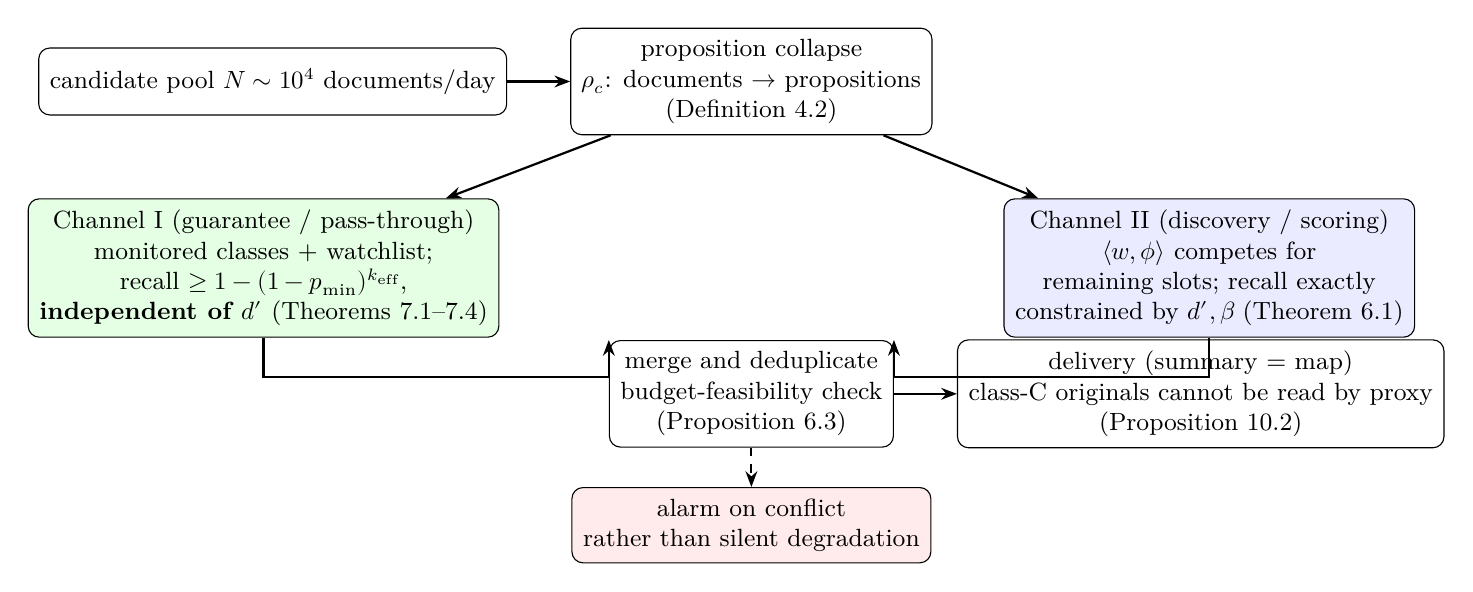
\begin{tikzpicture}[
  font=\small,
  box/.style={draw, rounded corners, align=center, minimum height=0.85cm, inner sep=4pt},
  chA/.style={box, fill=green!10},
  chB/.style={box, fill=blue!8},
  warn/.style={box, fill=red!8},
  arr/.style={-{Stealth[length=2mm]}, thick},
  node distance=0.6cm and 0.6cm]
\node[box] (pool) {candidate pool $N\sim 10^4$ documents/day};
\node[box, right=0.8cm of pool] (collapse) {proposition collapse\\ $\rho_c$: documents $\to$ propositions\\ (Definition 4.2)};
\node[chA, below left=0.8cm and 0.9cm of collapse] (ch1) {Channel I (guarantee / pass-through)\\ monitored classes + watchlist;\\ recall $\ge 1-(1-p_{\min})^{k_{\mathrm{eff}}}$,\\ \textbf{independent of $d'$} (Theorems 7.1--7.4)};
\node[chB, below right=0.8cm and 0.9cm of collapse] (ch2) {Channel II (discovery / scoring)\\ $\langle w,\phi\rangle$ competes for\\ remaining slots; recall exactly\\ constrained by $d',\beta$ (Theorem 6.1)};
\node[box, below=2.6cm of collapse] (merge) {merge and deduplicate\\ budget-feasibility check\\ (Proposition 6.3)};
\node[box, right=0.8cm of merge] (deliver) {delivery (summary = map)\\ class-C originals cannot be read by proxy\\ (Proposition 10.2)};
\node[warn, below=0.5cm of merge] (alarm) {alarm on conflict\\ rather than silent degradation};
\draw[arr] (pool) -- (collapse);
\draw[arr] (collapse) -- (ch1);
\draw[arr] (collapse) -- (ch2);
\draw[arr] (ch1.south) -- ++(0,-0.5) -| (merge.north west);
\draw[arr] (ch2.south) -- ++(0,-0.5) -| (merge.north east);
\draw[arr] (merge) -- (deliver);
\draw[arr, dashed] (merge) -- (alarm);
\end{tikzpicture}}
\caption{The dual-channel architecture: Channel I's recall guarantee comes from the redundant-coverage structure (independent of score separability); Channel II's recall contribution is honestly priced by the separability identity; the bottleneck theorem (Theorem 6.1) motivates this division of labor as one sufficient response within its model, not a universal architectural necessity.}
\end{figure}

\begin{center}\rule{0.5\linewidth}{0.5pt}\end{center}

\subsection{7 Redundant-Coverage Theorems: Structural Conditions and the
Applicability Domain of Recall under Aggressive
Filtering}\label{redundant-coverage-theorems-structural-conditions-and-the-applicability-domain-of-recall-under-aggressive-filtering}

The recall guarantee of Channel I (the guarantee channel) is supplied by
this section. The conditional design insight is that, in the regime
postulated by R1--R2, important information is redundantly covered
across source space. Consequently, the extremely aggressive filtering of
``retaining only the full content of a few trusted source classes''
still maintains provably high recall for critical propositions. This
section gives: (a) a complete proof for the independent case; (b) the
\textbf{independent-subset bound} for the correlated case together with
its \textbf{tightness}; (c) the dual optimization problem of
monitoring-slot allocation; (d) the total-recall theorem; (e) the
\textbf{applicability-domain boundary}---the strength of this section's
guarantee depends conditionally on the provenance of the coverage floor
\(p_{\min}\), and real-corpus pilots in two domains provide the first
version of this map (§7.5, §7.7).

\subsubsection{7.1 Assumptions}\label{assumptions}

\begin{itemize}
\tightlist
\item
  \textbf{R1 (Coverage floor)}: for every monitored trusted source class
  \(\mathcal{C}_i\) (\(i = 1,\dots,k\)) and every critical proposition
  \(e \in E^*\): \(P(Z_i(e) = 1) \ge p_{\min}\), where \(Z_i(e)\) is the
  coverage event of Definition 4.4. Empirical content: trusted source
  classes have a positive lower bound on their reporting rate for
  critical propositions; \(p_{\min}\) must be calibrated by measurement
  on historical corpora (Section 14), with conservative prior
  \(p_{\min} = 0.7\).
\item
  \textbf{R2 (Conditional independence)}: given the criticality of
  proposition \(e\), the coverage events \(\{Z_i(e)\}_{i=1}^k\) are
  mutually independent. Real-world deviation: shared wire-service
  upstreams and inter-media reposting networks induce positive
  correlation. Mitigation: source classes are partitioned by (ownership
  × geography × type) to constructively suppress cross-class correlation
  (Definition 4.4); the residual correlation is explicitly priced by
  Theorem 7.2.
\item
  \textbf{R3 (Pass-through rule)}: all authentic, correctly
  proposition-linked content of watchlist entities in
  \(\pi_{\mathrm{mon}}\) (companies, institutions, issues, and persons
  explicitly declared by the subject) bypasses competitive scoring and
  receives reserved Channel-I priority after deduplication, subject to
  R4.
\item
  \textbf{R4 (Realized pass-through feasibility)}: there is a
  probability-one event on which, \textbf{for every relevant period
  \(t\) and every proposition covered by an eligible monitored or
  watched source}, authentic ingestion, observation, provenance
  verification, correct proposition linking, deduplicated inclusion
  among the \(Q_{\mathrm I}(t)\) Channel-I propositions, reservation
  before Channel-II allocation, and \textbf{actual consumption} all
  hold, together with
  \(Q_{\mathrm I}(t)+m_{\mathrm{pub}}(t)+m_{\mathrm{slack}}(t)\le m(t)\).
  For a fixed proposition \(e\), only the corresponding probability-one
  subevent \(\mathcal D_e\) is required. R4 does not mean arrival,
  availability, or an expected-budget calculation alone. A feasibility
  alarm by itself does not constitute R4; entity silence, ingestion
  failure, verification failure, incorrect proposition linking, and
  overload are outside any zero-miss conclusion.
\end{itemize}

\subsubsection{7.2 The Independent Case}\label{the-independent-case}

\textbf{Theorem 7.1 (Redundancy coverage, independent case)}.
\emph{Under R1, R2, and R4, a filter that retains only the content of
\(k\) monitored source classes (direct pass-through after deduplication)
has, for any critical proposition \(e \in E^*\), miss probability
satisfying} \[P(\mathrm{miss}\, e) \ \le\ (1 - p_{\min})^k.\]

\textbf{Proof}. Proposition \(e\) is missed if and only if none of its
documents is consumed. Under R4, Channel I actually consumes all
eligible deduplicated content of the monitored classes, so a miss
\(\iff\) no monitored class covers \(e\)
\(\iff \bigcap_{i=1}^k \{Z_i(e) = 0\}\). By R2 (conditional
independence) and R1 (\(P(Z_i = 0) \le 1 - p_{\min}\)):
\[P(\mathrm{miss}\, e) = P\Big(\bigcap_{i=1}^k \{Z_i(e) = 0\}\Big) = \prod_{i=1}^k P(Z_i(e) = 0) \le (1 - p_{\min})^k. \qquad\blacksquare\]

\textbf{Numerics}: \(p_{\min} = 0.7\),
\(k = 5 \Rightarrow P(\mathrm{miss}) \le 0.3^5 = 2.43\times 10^{-3}\),
i.e., critical recall \(\ge 99.76\%\); even at \(p_{\min} = 0.5\),
\(k = 4\), one still has \(P(\mathrm{miss}) \le 6.25\times10^{-2}\).
\textbf{These are demonstration numbers for the independent case (where
R2 holds exactly), not a universal guarantee}: \(p_{\min}\) must be
calibrated by measurement (for the estimation procedure see §7.5 and
§14.7; confidence intervals should be reported), the correlated case
must switch to the \(k_{\mathrm{eff}}\) bound of Theorem 7.2, and the
measured \(\hat p_{\min} \approx 0.02\) of the academic-domain pilot is
precisely an instance of R1 failing (§7.7). Subject to this premise:
discarding 99\% of documents is fully compatible with retaining 99\%
critical recall---provided the retained 1\% is structurally selected
``by redundant coverage across source classes'' rather than
competitively selected by score. (Contrast Theorem 6.1: the latter route
requires \(d' \ge 4.39\).)

\subsubsection{7.3 The Correlated Case: The Independent-Subset Bound and
Its
Tightness}\label{the-correlated-case-the-independent-subset-bound-and-its-tightness}

R2 holds only approximately in reality. This subsection gives an upper
bound valid for \textbf{arbitrary dependence structures}, at the price
of reducing the exponent from \(k\) to the ``effective number of
independent classes.''

\textbf{Definition 7.1 (Effective number of independent classes)}. For a
fixed critical proposition \(e\), a subset \(S \subseteq [k]\) is called
\textbf{\(e\)-independent} if \(\{Z_i(e)\}_{i \in S}\) are mutually
independent. Define
\[k_{\mathrm{eff}}(e) := \max\{|S| : S \subseteq [k] \text{ is } e\text{-independent}\}, \qquad k_{\mathrm{eff}} := \min_{e \in E^*} k_{\mathrm{eff}}(e).\]

\textbf{Theorem 7.2 (Redundancy coverage, correlated case)}. \emph{Under
R1 and R4 (without assuming R2), for any critical proposition \(e\):}
\[P(\mathrm{miss}\, e) \ \le\ (1 - p_{\min})^{k_{\mathrm{eff}}(e)} \ \le\ (1 - p_{\min})^{k_{\mathrm{eff}}}.\]

\textbf{Proof}. Take an \(e\)-independent subset \(S^*\) attaining the
maximal cardinality in Definition 7.1, \(|S^*| = k_{\mathrm{eff}}(e)\).
Event inclusion: all \(k\) classes failing to cover \(\subseteq\) all
classes in \(S^*\) failing to cover, i.e.,
\[\{\mathrm{miss}\, e\} = \bigcap_{i=1}^k \{Z_i(e)=0\} \ \subseteq\ \bigcap_{i \in S^*} \{Z_i(e)=0\}.\]
By monotonicity of probability and independence on \(S^*\):
\[P(\mathrm{miss}\, e) \le P\Big(\bigcap_{i\in S^*}\{Z_i(e)=0\}\Big) = \prod_{i \in S^*} P(Z_i(e)=0) \le (1-p_{\min})^{|S^*|}. \qquad\blacksquare\]

\textbf{Proposition 7.1 (Tightness)}. \emph{Without further assumptions,
the bound of Theorem 7.2 cannot be improved: for each
\(k_{\mathrm{eff}} \in \{1, \dots, k\}\) there exists a dependence
structure satisfying R1 with
\(P(\mathrm{miss}\, e) = (1-p_{\min})^{k_{\mathrm{eff}}}\).}

\textbf{Proof}. First suppose \(0<p_{\min}<1\). Take
\(k_{\mathrm{eff}}\) groups of mutually independent classes, with the
\(Z_i\) within each group perfectly correlated (sharing a single latent
Bernoulli variable: media within a group share the same wire-service
upstream, \(Z_i\equiv Z_{\mathrm{group}}\),
\(P(Z_{\mathrm{group}}=1)=p_{\min}\)); groups are mutually independent.
Because each latent variable is nondegenerate, two distinct classes from
one group are not independent, whereas one class selected from each
group is independent. Thus Definition 7.1 gives exactly the number of
groups, and
\(P(\mathrm{miss})=P(\text{no group covers})=(1-p_{\min})^{k_{\mathrm{eff}}}\).
At \(p_{\min}=0\), the displayed bound is 1 and is trivially tight. At
\(p_{\min}=1\), every \(Z_i=1\) almost surely; deterministic variables
are independent of all others, so Definition 7.1 gives
\(k_{\mathrm{eff}}(e)=k\), the miss probability is 0, and the bound is
again tight. \(\blacksquare\)

\textbf{Engineering implications}: (a) the quality of the bound is
determined by \(k_{\mathrm{eff}}\), which can be enlarged only insofar
as the grouping design (ownership, geography, type, wire-service
upstream) creates certifiably independent classes---\textbf{independence
is a design target requiring validation, not a consequence of class
labels}; (b) historical correlation matrices and union-find merging of
pairs with \(|\rho_{ij}|>\epsilon_c\) may generate heuristic candidate
groups, but pairwise uncorrelatedness does not imply mutual
independence, and the merged-group count is neither a certificate nor a
rigorous lower or upper bound for \(k_{\mathrm{eff}}\). A candidate
independent subset needs a pre-specified joint-distribution or
generative-model independence argument; statistical dependence tests and
uncertainty intervals diagnose this model but do not by themselves prove
independence; (c) the substance of an astroturfing attack is the
fabrication of independence---multiple ``independent'' sources are in
fact a single actor. Defenses: root-node verification of the provenance
tree (I3) + ownership penetration + content-fingerprint clustering
(stress tests in Section 14).

\subsubsection{7.4 Watchlist Pass-Through and the Constructive Zeroing
of Tail
Risk}\label{watchlist-pass-through-and-the-constructive-zeroing-of-tail-risk}

\textbf{Proposition 7.2 (Conditional constructive zeroing under realized
feasibility)}. \emph{Let \(B_e\) be the event that an authentic document
concerning \(e\) is published by a watched entity, observed by the
ingestion system, provenance-verified, and correctly linked to \(e\).
Under R3 and R4, whenever \(P(B_e)>0\),}
\[P(\mathrm{miss}\,e\mid B_e)=0.\] \emph{Thus filtering introduces no
miss on \(B_e\). Entity silence, failure of ingestion or provenance
verification, incorrect proposition linking, and periods in which R4
fails are not zeroed. No unconditional zero-miss claim for every
watchlist proposition follows.}

\textbf{Proof}. On \(B_e\), the document enters \(Q_{\mathrm I}\) by R4;
R3 gives it reserved priority, and R4 reserves sufficient actual
consumption slots. Hence it is consumed rather than merely made
available. Proposition 6.3 supplies a feasibility warning, but only R4
turns that warning into a delivery guarantee. \(\blacksquare\)

\textbf{Sensitivity discussion} (explicit handling of the weakness of
R1): the soft underbelly of Theorems 7.1--7.2 is R1---\textbf{niche but
personally critical propositions lack source redundancy}
(\(P(Z_i(e)=1)\) is close to 0 for most classes). Three layers of
backstop: (1) on \(B_e\) and under R3--R4, pass-through constructively
zeroes the long-tail filtering risk that ``the subject can
foresee''---this is precisely how ``active acquisition'' complements
``passive filtering'': the watchlist is the subject's actively declared
projection of \(g^{(2)}\); (2) the public agenda layer (Section 12)
provides a second backstop for events ``unforeseen by the subject but
publicly momentous'' (redundantly attested propositions are forced into
everyone's view); (3) the scoring Channel II bears probabilistic
discovery (its recall contribution honestly priced by \(d'\)). Beyond
the three layers there remains an irreducible residual: propositions
with no trusted redundant sources, undeclared, not publicly momentous,
and undiscovered by scoring---this paper does not pretend it is zero,
but lists it as a measured audit item under P4 of Section 13.

\subsubsection{7.5 The Dual Problem: Monitoring-Slot
Allocation}\label{the-dual-problem-monitoring-slot-allocation}

The first decision on the active-acquisition side: \textbf{which source
classes to monitor?} Slots are limited (the budget constraint
\(m_{\mathrm{mon}}\), the pass-through quota constraint), candidate
classes outnumber slots, and selection is required.

\textbf{Definition 7.2 (Probabilistic coverage utility)}. Let
\(\mathcal{K}\) be the set of candidate classes, choose
\(S \subseteq \mathcal{K}\), \(|S| \le B\) (or a cost constraint
\(\sum_{i\in S} c_i \le B\)). A critical proposition \(e\) carries a
prior weight \(w_e\) (derived from the decision set declared by
\(g^{(2)}\)) and class coverage probabilities \(p_i(e) := P(Z_i(e)=1)\).
Define
\[U_{\mathrm{mon}}(S) := \sum_{e \in E^*} w_e \cdot P\big(e \text{ is covered by at least one class in } S\big) \;=\; \sum_{e} w_e \Big(1 - \prod_{i \in S}\big(1 - p_i(e)\big)\Big)\]
(the second equality uses R2 cross-class independence; for
arbitrary-dependence evaluation and the limits of product-based bounds,
see the remark).

\textbf{Theorem 7.3 (Submodularity of monitoring allocation and greedy
guarantees)}. \emph{\(U_{\mathrm{mon}}\) is monotone submodular. Hence:
under a cardinality constraint, greedy (adding at each step the class of
maximal marginal gain) attains \((1-1/e) \approx 63.2\%\) of optimal;
under a cost constraint, the better of density greedy and the best
single class attains \(\frac12(1-1/e)\) (folklore, see Leskovec et al.,
2007), and partial enumeration + density greedy attains \(1-1/e\)
(Sviridenko, 2004).}

\textbf{Proof}. No independence is needed for the set-function claim.
For each realization \(\omega\), define
\(F_e(S,\omega):=\max_{i\in S}Z_i(e,\omega)\), with the empty-set
maximum equal to zero. This is the monotone submodular coverage
function: adding a class cannot remove coverage, and its marginal gain
is no larger after other classes have already covered \(e\). Hence
\(P(e\text{ is covered by }S)=\mathbb E[F_e(S,\omega)]\) is monotone
submodular, and nonnegative weighting and summation over \(e\) preserve
both properties. The product expression in Definition 7.2 is only the
special evaluation under R2, not a prerequisite for monotonicity or
submodularity. The greedy guarantees cite Appendix B.4 together with
Sviridenko (2004) and Leskovec et al.~(2007), applied to the same
constraint and algorithm specifications. \(\blacksquare\)

\textbf{Remark (the correlated case)}. For two classes, nonnegative
covariance does imply
\(P(Z_1=1\lor Z_2=1)=p_1+p_2-P(Z_1=Z_2=1)\le p_1+p_2-p_1p_2\). Thus the
independence-product coverage formula is an \textbf{upper bound on
actual coverage}; equivalently, \((1-p_1)(1-p_2)\) is a \textbf{lower
bound on actual miss probability}, not a conservative recall lower bound
or miss-probability upper bound. For three or more classes, pairwise
positive correlation alone fixes no such direction. For example, let
\((P_{111},P_{110},P_{101},P_{011},P_{100},P_{010},P_{001},P_{000})=(.29,.01,.01,.01,.19,.19,.19,.11)\):
every marginal is \(.5\) and every pairwise intersection is \(.30>.25\),
yet the union probability is \(.89>.875=1-.5^3\). Without the joint law,
the product formula therefore has no universal one-sided conservative
interpretation for either coverage or miss probability. Theorem 7.3
still permits greedy optimization of the expected joint coverage without
that product. Theorem 7.2's maximum independent subset supplies a
miss-probability bound, not a partition into \(k_{\mathrm{eff}}\) groups
or a grouping-greedy rule; the latter requires a separately
pre-certified independent-group partition and group-level objective.
Astroturfing inflates \(U_{\mathrm{mon}}\) through ``pseudo-independent
groups''---for defenses see 7.3(c).

\textbf{Connection to Pandora's box}: Theorem 7.3 solves ``whom to
monitor among known classes''; \textbf{exploration when class quality is
unknown} (subscription trial and error) is the Pandora problem of
Section 8.3---the two together form the closed loop of the monitoring
list's life cycle: ``explore → admit → audit → rotate out.''

\textbf{Empirical Finding E-7.1 (The endogeneity of \(\hat p_{\min}\);
the academic-domain pilot)}. A researcher profile × real-corpus temporal
replay of arXiv 2019-09 (monitoring universe of 2,576 propositions;
observed proxy set \(E_{\mathrm{proxy}}\) = the month's top-2\%
most-cited papers, \(K^*=52\), rather than the formal ex-ante set
\(E^*(\tau)\); experimental details in §14.7) provides the first
measurement of the decisive role of list-construction strategy on
coverage: an author-granularity list (top-50 by prior-window frequency
or citation rank) covered only 1/52 of the month's critical papers
(\(\hat p_{\min}\approx0.02\))---the authors of the most important
papers such as ALBERT and Megatron-LM ranked beyond 1500th in the prior
window; an institution-granularity list (top-50 leading labs) gave
\(\hat p_{\min}=0.37\), and a trimmed top-10 list gave
\(\hat p_{\min}=0.17\) with supply matched to the budget.
\textbf{Conclusion: the \(p_{\min}\) of R1 is not an environmental
constant but a design function of list granularity and capacity}---the
construction of the monitoring list is itself a pull-side optimization
problem (the submodular greedy of Theorem 7.3 + the admission criterion
of Proposition 8.1 should be solved jointly, not by a top-N heuristic);
for low-redundancy profiles, the ceiling of Channel I's benefit is
determined by the diminishing margin of the capacity--coverage curve
(measured coverage rose only from 0.17 to 0.46 as list size went from 10
to 400---the measured ceiling of the list-coverage floor
\(\hat p_{\min}\), not end-to-end recall; at this configuration supply
far exceeds the budget, and quota dilution makes end-to-end recall lower
still). Note the limitation of the ground-truth proxy here: top-2\%
citation is a post-hoc indicator lagged by years and carrying prestige
bias; within this paper's own framework it is closer to ``academic
engagement'' than to ex ante criticality---§14.7 gives a sensitivity
discussion of this proxy.

\textbf{Empirical Finding E-7.2 (The institutional provenance of
\(p_{\min}\) and the dual-ground-truth split in \(d'\); the
financial-domain pilot)}. An investor profile × real-corpus temporal
replay of EDGAR + public news archives, 2019-09 (dual ground truth:
legally material 8-Ks and market-moving days; experimental details in
§14.7) supplies the other half of the applicability-domain map: (a)
\textbf{\(p_{\min}\) can have an institutional provenance}: the
regulatory primary-source class's coverage of the legal ground truth
(material 8-Ks) is \(\hat p_{\min} = 1.00\)---the four-day filing rule
provides an institutional reason for high coverage of this legally
defined filing proxy, not a guarantee of ex-ante availability or of
arbitrary decision-critical information; against the market ground
truth, \(\hat p_{\min}=0.70\)--\(0.73\) (depending on the news-layer
version; see the caliber comparison in Table 14-3), and wire-service
classes add a further \textasciitilde0.25--0.27 of independent
coverage---\textbf{a multi-class redundancy structure
(\(k_{\mathrm{eff}}\ge2\)) becomes measurable on real data for the first
time}; (b) \textbf{the honest-feature scorer's \(d'\) splits by ground
truth}: legal criticality is predictable from disclosure metadata
(\(d'=2.65\)--\(3.49\), depending on the feature-set version), while
market criticality is only partially predictable from realized attention
signals (\(d'=0.54\)--\(0.60\))---both far below the 95\%-recall
requirement line (≈4.4); criticality on the market dimension is borne
\textbf{mainly} by structure, a same-corpus pattern consistent with
Theorem 6.1's model-specific thesis, not independent confirmation; (c)
\textbf{a favorable historical proxy configuration crosses 0.95 only
before news-layer expansion}: portfolio-holdings pass-through (25
holdings, supply of 4.6 propositions/day), under quota-matched
conditions, showed within-portfolio market-ground-truth recall climbing
with the budget: 0.444 at \(m=1\) → 0.952 at \(m=5\) (meeting the
target); after the news-layer expansion, a different configuration
diluted to 0.910 (within-portfolio targets 18→19; supply 4.6→4.733
propositions/day) (the news propositions of company-days drew away
quota---``approaching but not crossing the line''; fulfillment requires
raising the quota or strengthening within-list ranking). Contrasted with
the academic domain (where under the same framework and methods the
strong form was rejected, best end-to-end recall 0.28), this yields a
first empirical regularity: \textbf{recall-guarantee strength = the
institutional provenance of \(p_{\min}\) (law \textgreater{} media
redundancy \textgreater{} list design) × supply--quota fit × the
consistency between the scope of \(E^*\) and the profile's decision
set}. Again note the ground-truth proxy limitation: market-moving days
are post-hoc labels, and 90\% of market-moving days are not attributable
to same-day information---``recall of market-moving days'' does not
equal ``recall of ex ante critical information''; §14.7 gives the second
ground truth and the sensitivity analysis.

\subsubsection{7.6 The Total-Recall
Theorem}\label{the-total-recall-theorem}

\textbf{Theorem 7.4 (Per-proposition total-recall bound, with
actual-consumption events)}. \emph{Fix \(e\in E^*\setminus\mathrm{WL}\).
For \(J\in\{\mathrm I,\mathrm{II}\}\), let \(D_J(e)\) be the event that
Channel \(J\) \textbf{actually consumes} proposition \(e\), and define
\(F_{\mathrm I}(e):=D_{\mathrm I}(e)^c\), \(q_e:=P(F_{\mathrm I}(e))\),
and \(\mathrm{miss}(e):=D_{\mathrm I}(e)^c\cap D_{\mathrm{II}}(e)^c\).
Delivery, recovery, and miss therefore have one common
actual-consumption meaning. Whenever \(q_e>0\), define the
proposition-specific conditional recovery probability}
\[R_{\mathrm{II}}(e):=P(D_{\mathrm{II}}(e)\mid F_{\mathrm I}(e)).\]
\emph{Under R1 and R4,}
\[P(\mathrm{miss}\,e)=q_e[1-R_{\mathrm{II}}(e)]\le(1-p_{\min})^{k_{\mathrm{eff}}(e)}[1-R_{\mathrm{II}}(e)]\le(1-p_{\min})^{k_{\mathrm{eff}}}[1-R_{\mathrm{II}}(e)].\]
\emph{If \(q_e=0\), the miss probability is zero and
\(R_{\mathrm{II}}(e)\) need not be defined. If a uniform lower bound
\(R_{\mathrm{II}}^{\inf}:=\inf_{e\in E^*\setminus\mathrm{WL}:q_e>0}R_{\mathrm{II}}(e)\)
is certified, \(1-R_{\mathrm{II}}(e)\) may be replaced by
\(1-R_{\mathrm{II}}^{\inf}\). In particular, the weaker recovery-free
bound \(P(\mathrm{miss}\,e)\le(1-p_{\min})^{k_{\mathrm{eff}}}\) remains
valid. No independence between Channels I and II is assumed. For
\(e\in E^*\cap\mathrm{WL}\), zero miss holds only conditional on \(B_e\)
and R4 as in Proposition 7.2; without that event, the applicable general
bound is the redundancy bound, not zero.}

\textbf{Proof}. The equality follows from the chain rule applied
separately to each \(e\in E^*\setminus\mathrm{WL}\) and the common event
definitions. The first inequality uses Theorem 7.2 with
\(k_{\mathrm{eff}}(e)\) and R4's actual-consumption subevent for \(e\);
the second uses \(k_{\mathrm{eff}}\le k_{\mathrm{eff}}(e)\). The
uniform-bound statement follows from
\(R_{\mathrm{II}}^{\inf}\le R_{\mathrm{II}}(e)\), and the recovery-free
bound from \(R_{\mathrm{II}}(e)\ge0\). \(\blacksquare\)

\textbf{Remark (pooled averages, estimation, and selection bias)}. A
pooled conditional recovery average is not a per-proposition lower
bound. For example, if Channel I has failure probability \(0.5\) for
\(e_1,e_2\), Channel II always recovers \(e_1\) and never recovers
\(e_2\) after Channel-I failure, then pooled \(R_{\mathrm{II}}=0.5\),
but \(P(\mathrm{miss}\,e_2)=0.5\), violating the former pooled bound
\(0.25\). The correct aggregate statement over
\(e\in E^*\setminus\mathrm{WL}\) is failure-weighted: if \(w_e\ge0\),
\(Q:=\sum_ew_eq_e>0\), and
\(\bar R_{\mathrm{II},q}:=Q^{-1}\sum_ew_eq_eR_{\mathrm{II}}(e)\), then
\(\sum_ew_eP(\mathrm{miss}\,e)=(1-\bar R_{\mathrm{II},q})\sum_ew_eq_e\),
with the convention \(q_eR_{\mathrm{II}}(e):=0\) when \(q_e=0\); this
says nothing pointwise. Moreover, Theorem 6.1 does not determine
\(R_{\mathrm{II}}(e)\) from \(d'\) and \(\beta\) alone, because those
parameters describe the unconditional scoring population rather than the
Channel-I-failure subpopulation. Conditional per-proposition estimates
or a certified uniform lower bound are required; the recovery-free bound
needs no such estimate.

\textbf{KPI implementation}: the simulations and synthetic ecology
(Section 14) measure \(P(\mathrm{miss})\) directly and compare it
against \((1-\hat p_{\min})^{\hat k_{\mathrm{eff}}}\); the
\textbf{real-corpus temporal replay} (§14.7) deterministically computes
misses against frozen retrospective proxy lists (H4'); this does not
measure ex-ante critical recall or point-in-time availability;
human-jury audits remain in the postponed L3 design (§15.5).

\subsubsection{7.7 Applicability-Domain Boundaries and Claim Calibration
(An Honest
Summary)}\label{applicability-domain-boundaries-and-claim-calibration-an-honest-summary}

The relationship between the strength of this section's theorems and
their own pilot evidence must be understood according to the following
calibration---this is the central calibration of the paper's empirical
claims:

\begin{enumerate}
\def\labelenumi{\arabic{enumi}.}
\tightlist
\item
  \textbf{The theorem guarantee is conditional}. The numerical comfort
  of \(P(\mathrm{miss}) \le (1-p_{\min})^{k_{\mathrm{eff}}}\) (e.g.,
  \(p_{\min}=0.7, k=5 \Rightarrow 99.76\%\)) comes from the universal
  quantification of R1 (for \textbf{every} \(e \in E^*\),
  \(P(Z_i)\ge p_{\min}\)). The pilots show that \(\hat p_{\min}\) is a
  strong function of list granularity and capacity: author-granularity
  lists go as low as \(\hat p_{\min}\approx0.02\), at which point the
  \((1-\hat p_{\min})^k\) bound is vacuous (\(0.98^5\approx0.90\)); the
  only source of \(\hat p_{\min}=1.00\) is a \textbf{legal institution}
  such as the four-day filing rule for 8-Ks, not the framework itself.
\item
  \textbf{Pointwise and aggregate outputs are distinct}. The pointwise
  bounds of Theorems 7.1--7.4 require R1 for every proposition in their
  stated \(E^*\) and R4 for realized delivery. Separately, when no
  uniform coverage floor is available, we report only aggregate weighted
  leakage \(L_w(S):=\sum_ew_e\prod_{i\in S}(1-p_i(e))\), with the
  required independence structure and realized-delivery accounting
  explicit. This aggregate quantity guides monitoring-slot optimization;
  it is not a pointwise recall guarantee and does not weaken the
  hypotheses of the pointwise theorems. Choosing the aggregate
  deployment objective therefore does not ``repair'' an R1 failure for
  Theorem 7.4.
\item
  \textbf{The correct statement of ``≥95\% recall''}: a formal target
  requires the joint coverage, independence, R4 list--budget fit,
  publication/ingestion/linkage, and decision-set scope conditions.
  Empirically, 0.952 was attained only for the favorable historical
  financial within-portfolio market-day proxy configuration, while 0.910
  occurred after changing that configuration and its target denominator;
  neither estimates ex-ante critical recall. The academic best 0.28
  rejects the 95\% target for its tested citation proxy, not for an
  independently elicited ex-ante target. All recall figures must
  therefore carry both their proxy and their configuration.
\item
  \textbf{Robustness ledger beyond the stated assumptions (non-Gaussian
  criticality, heavy tails, correlated coverage, correlated scores)}.
  (i) \emph{Distribution-freeness of Theorems 7.1--7.2}: the coverage
  events are Bernoulli; the bounds depend only on the per-class coverage
  probabilities and the independence structure, and make \textbf{no}
  Gaussianity or light-tail assumption anywhere. Heavy-tailed
  criticality (the Pareto exponent \(\alpha\) of §14.1) enters only
  through the \textbf{estimation} of \(p_{\min}\); since the miss bound
  is monotone in \(1-p_{\min}\), the only dangerous error direction is
  overestimating \(p_{\min}\), which is why the confidence-adjusted form
  is the deployment form: with \(n\) class-coverage observations per
  class, substituting the Clopper--Pearson lower bound \(p_L\) (level
  \(1-\alpha\)) for \(\hat p_{\min}\) makes
  \(P(\mathrm{miss}) \le (1-p_L)^{k_{\mathrm{eff}}}\) a
  \(1-\alpha\)-confidence statement; the pilot effect-size tables report
  \(p_L\) alongside \(\hat p_{\min}\). (ii) \emph{Correlated coverage}
  is priced under \textbf{arbitrary} correlation by Theorem 7.2:
  \(k_{\mathrm{eff}}\) is the size of the largest class subset with
  guaranteed-independent coverage events; the correlation-shock stress
  test §14.5(a) measures the degradation of \(k_{\mathrm{eff}}\) under a
  shared-upstream merger, and regrouping by ownership/geography/type is
  the designed repair. (iii) \emph{Score-distribution robustness of the
  bottleneck (Theorem 6.1)}: the numeric line \(d' \ge 4.39\) is a
  Gaussian specialization; the \textbf{distribution-free} content is the
  quantile criterion obtained by writing the threshold test with the
  true class-conditional laws \(P_0\) (noncritical) and \(P_1\)
  (critical): recall \(R\) at consumption rate \(\beta\) via threshold
  \(z\) requires \(P_1(s > z) = R\) and
  \(P_0(s > z) = (\beta - \pi R)/(1-\pi)\); hence 95\% recall at
  \(\beta = 1.25\pi\) is attainable \textbf{iff}
  \(P_0\big(s > Q_1(0.95)\big) \le (\beta - 0.95\pi)/(1-\pi) = 0.00303\),
  where \(Q_1\) is the critical-score quantile function---i.e., the
  threshold capturing 95\% of critical mass may leave at most 0.303\% of
  noncritical mass above it. Under Gaussian scores with separation
  \(d'\) this evaluates to \(d' \ge 4.39\); under heavy-tailed or skewed
  scores it evaluates with their own quantiles, and the qualitative
  thesis---\textbf{at extreme filtering ratios recall is carried by the
  tail overlap of the score distributions, not by scorer quality}---is
  unchanged; the measured separations (\(d'\) 0.54--3.49 across two
  domains and two ground truths) fail the criterion under either
  evaluation. (iv) \emph{The institutional provenance of \(p_{\min}\) is
  the core boundary of the recall guarantee, not an ancillary caveat}:
  law (\(\hat p_{\min}=1.00\)) \textgreater{} media redundancy
  (0.70--0.73) \textgreater{} list design (0.02--0.37), and the strength
  ordering of every recall claim in this paper is exactly this
  provenance ordering (E-7.1/E-7.2); any deployment claim of high recall
  must first declare the provenance of its \(p_{\min}\).
\end{enumerate}

\begin{center}\rule{0.5\linewidth}{0.5pt}\end{center}

\subsection{8 A Theory of Active Acquisition (Pull) and the Attention
No-Arbitrage
Theorem}\label{a-theory-of-active-acquisition-pull-and-the-attention-no-arbitrage-theorem}

This section takes up the third of the four questions: ``Beyond
filtering, what should be actively acquired, how much, and when should
one stop?'' The classical traditions surveyed in Section 2.7 (search,
foraging, experimental design, bandits, optimal stopping) are woven here
into the pull side of the SAP and brought, by the \textbf{attention
no-arbitrage theorem} (Theorem 8.1), under an organizing KKT price whose
relation to push and reflection requires the unit conversions stated
below. A caveat is in order: mathematically, Theorem 8.1 is a direct
application of the KKT conditions for concave programming; its
contribution is organizational: \textbf{the marginal value theorem,
Pandora's stopping rule, and the consumption threshold can be compared
through one variational principle only after their distinct units,
active sets, and model reductions are made explicit}. This turns budget
allocation into a control problem without claiming that every classical
index equals the same scalar.

\subsubsection{8.1 The Space of Pull
Operators}\label{the-space-of-pull-operators}

\textbf{Definition 8.1 (Pull operators)}. In each period, an
active-acquisition policy \(\pi_{\mathrm{pull}}\) selects a combination
of three classes of operators:

\begin{itemize}
\tightlist
\item
  \textbf{Exploration operator} \(e\): a trial investment in a candidate
  source \(s \notin \pi_{\mathrm{mon}}\) (reading its historical
  content, a small-sample subscription), at cost \(c_e\) (minutes), with
  reward \(X_s^H\) (the source's discounted total utility over a
  declared horizon \(H\), estimated with noise; §8.3 supplies the
  required conversion from daily rates);
\item
  \textbf{Query operator} \(q\): targeted retrieval (keywords, lateral
  reading, database queries, delegating subtasks to AI agents), at cost
  \(c_q\), with reward the query's expected information gain
  \(\mathrm{EIG}(q \mid K)\) relative to the decision set \(D\) and the
  knowledge state \(K\);
\item
  \textbf{Dwelling operator}: continued reading of an already-subscribed
  source (a patch), dwelling for a duration \(t\) with cumulative reward
  \(G_s(t)\) (concave: the first few items capture most of the value,
  with diminishing margins thereafter).
\end{itemize}

The total pull cost per period,
\(c(\pi_{\mathrm{pull}}) = \sum c_e + \sum c_q + \sum t\), enters the
budget identity
\(T = T_{\mathrm{pull}} + T_{\mathrm{push}} + T_{\mathrm{ref}}\).

\subsubsection{8.2 The Attention No-Arbitrage
Theorem}\label{the-attention-no-arbitrage-theorem}

\textbf{Setup}. Allocate the budget \(T\) across \(U\) uses (push
consumption, the various pull operators, reflection); use \(u\) receives
\(x_u \ge 0\) minutes and yields expected value \(V_u(x_u)\). Assume:

\begin{itemize}
\tightlist
\item
  \textbf{(P1) Concavity}: \(V_u\) is increasing, concave, and
  continuously differentiable. Economic rationale: redundancy---the
  first few items of a source capture most of its value (the
  expectation-level manifestation of the submodularity of the coverage
  utility); the marginal EIG of queries is diminishing (the
  submodularity of Theorem 8.2); the marginal virtue gain of reflection
  is diminishing (the drift structure of Section 10).
\item
  \textbf{(P2) Separability}: \(V(x) = \sum_u V_u(x_u)\) (no interaction
  across uses). Idealization: complementarities (retrieval results
  change the novelty baseline of push scoring) do exist and are treated
  as second-order terms; the simulations (Section 14) include
  interaction stress tests.
\end{itemize}

\textbf{Theorem 8.1 (KKT characterization of attention allocation)}.
\emph{Under (P1)--(P2), a feasible allocation \(x^*\) with
\(\sum_ux_u^*=T\) is optimal if and only if there exists \(\nu\ge0\)
such that every funded use (\(x_u^*>0\)) satisfies \(V_u'(x_u^*)=\nu\),
and every unfunded use (\(x_u^*=0\)) satisfies \(V_u'(0)\le\nu\). If a
funded use has strictly positive marginal value, then \(\nu>0\).}

\emph{Corollary (no arbitrage only on feasible transfer directions). All
funded uses have the same marginal value, but an unfunded use may have a
strictly smaller marginal value. If \(x_{u'}^*>0\) and
\(V_u'(x_u^*)>V_{u'}'(x_{u'}^*)\), transferring sufficiently small
\(\epsilon>0\) from \(u'\) to \(u\) is feasible and yields first-order
gain \(\epsilon(V_u'-V_{u'}')+o(\epsilon)>0\). No transfer ``out of'' an
unfunded use exists, and no equality between funded and unfunded uses is
required beyond the KKT inequality.}

\textbf{Proof}. Necessity: suppose \(x^*\) is optimal and there exist
interior uses \(u, u'\) with \(V_u'(x_u^*) > V_{u'}'(x_{u'}^*)\). Take
\(\epsilon > 0\) sufficiently small and set \(x'_u = x_u^* + \epsilon\),
\(x'_{u'} = x_{u'}^* - \epsilon\), all else unchanged (feasibility:
interiority + budget conservation). By differentiability,
\[V(x') - V(x^*) = \big[V_u(x_u^*+\epsilon) - V_u(x_u^*)\big] + \big[V_{u'}(x_{u'}^*-\epsilon) - V_{u'}(x_{u'}^*)\big] = \epsilon\big(V_u'(x_u^*) - V_{u'}'(x_{u'}^*)\big) + o(\epsilon) > 0\]
for sufficiently small \(\epsilon\), contradicting optimality. The
corner condition is analogous (if \(V_u'(0) > \nu = V_{u'}'(x_{u'}^*)\),
moving in yields a positive gain). Sufficiency: suppose there exists a
\(\nu\) for which the conditions hold. For any feasible \(x\), concavity
gives \(V_u(x_u) \le V_u(x_u^*) + V_u'(x_u^*)(x_u - x_u^*)\); summing,
\[V(x) - V(x^*) \le \sum_u V_u'(x_u^*)(x_u - x_u^*) \le \nu \sum_u (x_u - x_u^*) = \nu\,(T - T) = 0.\]
The second inequality is an equality for funded uses; at a corner
\(x_u^*=0\), it follows from \(V_u'(0)\le\nu\) and \(x_u\ge0\). Hence
\(x^*\) is globally optimal. \(\blacksquare\)

\textbf{The organizing power of Theorem 8.1}: the following three
classical rules are all special cases of the variational principle
``marginal value = shadow price \(\nu\)''---

\begin{longtable}[]{@{}
  >{\raggedright\arraybackslash}p{(\linewidth - 4\tabcolsep) * \real{0.3333}}
  >{\raggedright\arraybackslash}p{(\linewidth - 4\tabcolsep) * \real{0.3333}}
  >{\raggedright\arraybackslash}p{(\linewidth - 4\tabcolsep) * \real{0.3333}}@{}}
\toprule\noalign{}
\begin{minipage}[b]{\linewidth}\raggedright
Classical rule
\end{minipage} & \begin{minipage}[b]{\linewidth}\raggedright
Source
\end{minipage} & \begin{minipage}[b]{\linewidth}\raggedright
Role within SEA
\end{minipage} \\
\midrule\noalign{}
\endhead
\bottomrule\noalign{}
\endlastfoot
Patch rule: compare the instantaneous marginal rate \(G_s'(t)\), not
generally the cycle average, with \(\nu\) & Charnov (1976), Proposition
8.2 & a time-rate comparison for the dwelling operator \\
Pandora stopping: in total-utility units, do not open boxes with
\(z_s^H<B_0^H\); convert \(\nu c_e\) before computing \(z_s^H\) &
Weitzman (1979), Proposition 8.1 & exploration after
total-value/time-rate conversion \\
Push threshold: \(r(s)\ge\tau_i(b)\) in utility/slot; with \(\ell\)
minutes per slot and \(\tau_i(b)=\nu\ell\), equivalently
\(r(s)/\ell\ge\nu\) & Proposition 6.4 & filtering after slot-to-minute
conversion \\
\end{longtable}

\textbf{Status of Theorem 8.1 (a unification theorem, not a new
mathematical discovery---stated explicitly in v1.6)}. The
marginal-equality condition is the KKT/variational characterization of
an optimum of a concave budget-allocation problem, and that Charnov's
marginal-value rule and Weitzman's Pandora rule are instances of one
underlying optimization principle is known in substance (Charnov, 1976;
Weitzman, 1979). The contribution claimed here is \textbf{taxonomic and
organizational}: funded uses inside the concave time-allocation problem
share one KKT price, while slot thresholds, total-utility Pandora
indices, patch-cycle averages, and Whittle indices enter only after
their explicit unit conversions and model reductions. The theorem does
not identify every threshold numerically with \(\nu\), does not assert a
previously unknown mathematical relation, and does not make the
monitoring rotation heuristic a consequence of Weitzman's theorem.

\textbf{Engineering implications and loss order}: the scheduler
estimates marginal VOI for funded uses and checks KKT inequalities
before activating unfunded uses. If \(\nabla V\) is \(L\)-Lipschitz, the
correct smoothness bound for feasible \(x\) is
\(V(x^*)-V(x)\le-\nabla V(x^*)^\top(x-x^*)+\tfrac L2\|x-x^*\|^2\). For a
transfer of \(\epsilon\) from funded use \(u'\) to a previously
zero-budget use \(u\), the first-order loss is
\((\nu-V_u'(0))\epsilon\). It vanishes \textbf{when the activated
zero-budget use satisfies \(V_u'(0)=\nu\)}, not only for reallocations
among funded uses; when \(V_u'(0)<\nu\), there is generally a
first-order loss \((\nu-V_u'(0))\epsilon+O(\epsilon^2)\). A universal
\(\Theta(\epsilon^2)\) claim would therefore be false even though
second-order loss can occur at a boundary-active KKT point. Explicitly,
on \(x_1+x_2=1\), take \(V_1=2x_1-\tfrac12x_1^2\) and
\(V_2=x_2-\tfrac12x_2^2\). The global optimum is \(x^*=(1,0)\), with
\(V_1'(1)=V_2'(0)=\nu=1\); activating use 2 by transferring \(\epsilon\)
gives \(V(x^*)-V(1-\epsilon,\epsilon)=\epsilon^2\) exactly, with zero
first-order term. By contrast, \(V_1=x_1\), \(V_2=2x_2\) has optimum
\((0,1)\), unequal marginals \(1<2\), and loss \(\epsilon\) from
reallocating \(\epsilon\) to use 1. Thus ``approximate scheduling is
second-order'' is not a general guarantee.

\subsubsection{8.3 Source Exploration: Pandora's Box and Monitoring
Admission}\label{source-exploration-pandoras-box-and-monitoring-admission}

\textbf{Theorem (Weitzman, 1979; classical result, cited)}. \emph{\(n\)
boxes; box \(i\) costs \(c_i>0\) to open and contains an independent
integrable random reward \(X_i\sim F_i\); after opening, one may take
the maximum reward among opened boxes and stop, or continue opening.
Define the reservation index \(z_i\) by \(\mathbb E[(X_i-z_i)^+]=c_i\).
Under Weitzman's independence and stationarity assumptions, the optimal
policy opens boxes in descending order of \(z_i\) and stops when the
best opened reward is at least the maximum remaining index.}

(For \(c_i>0\), the left-hand side is continuous, strictly decreasing
where positive, tends to \(+\infty\) as \(z_i\to-\infty\), and tends to
zero as \(z_i\to+\infty\), giving a unique solution. For \(c_i=0\),
every \(z\ge\operatorname{ess\,sup}X_i\) satisfies the equation; the
canonical zero-cost index is defined by convention as
\(\operatorname{ess\,sup}X_i\), not inferred to be unique from the
equation. For the optimality proof see Weitzman (1979).)

\textbf{Proposition 8.1 (Pandora exploration in total-utility units,
with separate resource-constrained admission)}. \emph{Fix a common
evaluation horizon \(H\). Let \(X_s^H\) be discounted total utility from
monitoring source \(s\) over \(H\), and let \(B_0^H\) be discounted
total utility of the best existing use over the same horizon.
Exploration takes \(c_e\) minutes. For the exact model, \(c_e\),
\(\widetilde c_e\), and \(B_0^H\) must be deterministic and fixed before
exploration begins, with opening costs independent of all box rewards.
Either \(\nu\) is a known deterministic constant during exploration and
\(\widetilde c_e:=\nu c_e\), or \(\nu(t)\) is a \textbf{deterministic
path known before opening}, independent of exploration outcomes and the
policy path, and the actual additive utility-denominated opening cost is
exactly \(\widetilde c_e:=\int_0^{c_e}\nu(t)dt\). If \(\nu\) is only
approximately constant, \(\nu c_e\) is a heuristic index approximation
and no exact optimality or error bound is claimed. If \(\nu(t)\) or
\(c_e\) is random, reward-dependent, or adapted to opened results or the
policy path, replacing the cost by its integral or expectation does
\textbf{not} preserve classical fixed-cost Weitzman optimality; that
case requires a separate stochastic-cost stopping model. Define
\(z_s^H\), in total-utility units, by}
\[\mathbb E[(X_s^H-z_s^H)^+]=\widetilde c_e.\] \emph{(i) Add a zero-cost
outside-option box with deterministic total reward \(B_0^H\). Under
Weitzman's independence and stationarity assumptions, exploration
follows descending \(z_s^H\), and boxes with \(z_s^H<B_0^H\) are not
opened. These total-utility thresholds are not numerically identical to
the rate \(\nu\).}

\emph{(ii) Actual monitoring admission is a separate
resource-constrained decision. If source \(s\) requires \(a_s\)
monitoring minutes per day and yields expected value \(\bar v_s\) per
day, its attention-rate comparison is \(\bar v_s/a_s\ge\nu\). Slot
conflicts are resolved jointly with the coverage objective of Theorem
7.3 and R4; no single realized \(X_s^H\) comparison is an iff admission
rule.}

\emph{(iii) A rolling \(L\)-period rotation recommendation is a
heuristic governance rule requiring human sign-off, not a consequence of
time-reversing Weitzman's theorem.}

\textbf{Proof and free-box convention}. Part (i) is Weitzman's theorem
after all rewards and costs have been converted to total utility over
\(H\). The deterministic zero-cost box \(X_0=B_0^H\) is assigned the
canonical index \(z_0=B_0^H\) using the essential-supremum convention
above. Although every \(z\ge B_0^H\) satisfies
\(\mathbb E[(B_0^H-z)^+]=0\), uniqueness must not be inferred from that
equation. Parts (ii)--(iii) are additional resource and governance
rules, not steps of Weitzman's optimality proof. \(\blacksquare\)

\textbf{Remark}: when \(X_s\) is non-stationary (source-quality drift),
the stationary Pandora assumption fails; the remedy is rolling-window
estimation + drift detection (CUSUM), and the theory falls under the
restless-bandit framework of Section 8.6.

\subsubsection{8.4 Patch Dwelling: The Marginal-Value
Rule}\label{patch-dwelling-the-marginal-value-rule}

\textbf{Proposition 8.2 (Patch dwelling with unit-consistent switching
costs)}. \emph{The cumulative information reward of source \(s\) is
\(G_s(t)\), with \(G_s(0)=0\), increasing, differentiable, and concave.
A fixed switching loss \(\kappa_{sw}\) measured in \textbf{utility} and
a switching time \(\tau_{sw}\) measured in \textbf{minutes} are
alternative specifications and must not be mixed. Respectively,}
\[R_\kappa(t):=\frac{G_s(t)-\kappa_{sw}}t,\qquad R_\tau(t):=\frac{G_s(t)}{t+\tau_{sw}}.\]
\emph{At an interior average-rate maximizer,}
\[G_s'(t^*)t^*=G_s(t^*)-\kappa_{sw},\qquad\text{or}\qquad G_s'(t^*)(t^*+\tau_{sw})=G_s(t^*),\]
\emph{so in either specification \(G_s'(t^*)=R(t^*)\) under the
corresponding definition of \(R\).}

\emph{The further equality \(R(t^*)=\nu\) holds only when \(\nu\) is
defined as the endogenous long-run environmental average of the
stationary patch-cycle model. It is not an unconditional consequence of
Theorem 8.1. If \(\nu\) is instead an exogenous outside-option price and
the average-rate-maximizing \(t^*\) has \(R(t^*)>\nu\), then
\(G_s'(t^*)=R(t^*)>\nu\); extending beyond \(t^*\) can improve net value
relative to the outside option. \textbf{For an entered patch with a
finite interior stopping optimum}, stopping satisfies \(G_s'(t)=\nu\);
boundary optima instead stop immediately, continue indefinitely, or
decline entry.}

\textbf{Proof}. Differentiating \(R_\kappa\) and \(R_\tau\) gives,
respectively,
\[R_\kappa'(t)=\frac{G_s'(t)t-[G_s(t)-\kappa_{sw}]}{t^2},\qquad R_\tau'(t)=\frac{G_s'(t)(t+\tau_{sw})-G_s(t)}{(t+\tau_{sw})^2}.\]
Setting each numerator to zero gives the two tangency conditions and
hence \(G_s'=R\) at the corresponding interior maximizer. Concavity
supplies the usual quasi-concavity argument under the stated boundary
conditions. The outside-option comparison uses instantaneous marginal
value per minute, which is the unit of \(\nu\); it does not identify an
arbitrary cycle average with \(\nu\). \(\blacksquare\)

\textbf{Boundary cases (utility-cost specification only)}. Write
\(h(t):=G_s(t)-tG_s'(t)\). An interior stationary point requires
\(h(t)=\kappa_{sw}\); for a global interior maximizer under the stated
quasi-concavity conditions, \(R_\kappa'\) must change from positive to
negative at that crossing (equivalently, \(\kappa_{sw}-h(t)\) must cross
from positive to negative). The single inequality
\(\kappa_{sw}<\sup_t h(t)\) is not a universal iff: when
\(\kappa_{sw}=0\), \(G_s(t)=1-e^{-t}\) gives
\(R_\kappa(t)=(1-e^{-t})/t\), which is strictly decreasing and has no
finite interior maximizer; equality \(\kappa_{sw}=\sup h\) can also be
attained on a plateau. Immediate stopping, indefinite continuation, and
non-entry must therefore be evaluated separately. This crossing analysis
is not transferred to \(R_\tau\) without a separate derivation.

\textbf{This is information foraging made normative}: the descriptive
``information-scent following'' of Pirolli \& Card (1999) acquires in
SEA an explicit stopping rule; the engineering identity of ``scent'' is
an online estimate of \(G_s'(\cdot)\) (rolling proxies of click depth
and content novelty).

\subsubsection{8.5 Query Batches: The Submodularity of Expected
Information
Gain}\label{query-batches-the-submodularity-of-expected-information-gain}

\textbf{Setup}. A query set \(\mathcal{Q}\) (candidate queries,
retrieval expressions, lateral-reading targets), each \(q\) with cost
\(c_q\), returns an observation \(Y_q\) (a noisy signal about
\(\Theta_{\mathrm{rel}}\)). The value of a batch
\(Q \subseteq \mathcal{Q}\) is \(I(Q) := I(Y_Q;\, \omega \mid K)\)
(conditional mutual information given the current knowledge state). The
submodular structure of such problems has been systematically studied in
sensor-network placement (Krause, Singh \& Guestrin, 2008); this paper
transplants it to the cognitive-budget setting.

\textbf{Theorem 8.2 (Monotonicity of EIG and submodularity under
conditional independence)}.

\emph{(i) (Monotonicity, no additional assumptions) \(I(Q)\) is monotone
nondecreasing in \(Q\).}

\emph{(ii) (Submodularity) If the observations are conditionally
independent given \(\omega\) (\(Y_q \perp Y_{q'} \mid \omega\)), then
\(I(Q)\) is submodular.}

\emph{(iii) (Guarantees) With equal costs, greedy attains \((1-1/e)\)
(Nemhauser et al., 1978); under a cost constraint, the better of density
greedy and the best single query attains \(\frac12(1-1/e)\) (Leskovec et
al., 2007), and partial enumeration + density greedy attains \((1-1/e)\)
(Sviridenko, 2004).}

\textbf{Proof}. (i) Chain rule and nonnegativity of mutual information:
for \(q \notin Q\),
\[I(Q \cup q) - I(Q) = I(Y_q;\, \omega \mid Y_Q) \ \ge\ 0.\]

\begin{enumerate}
\def\labelenumi{(\roman{enumi})}
\setcounter{enumi}{1}
\item
  The gain is \(\Delta(Q, q) := I(Y_q; \omega \mid Y_Q)\). Under the
  conditional-independence assumption,
  \[\Delta(Q,q) = H(Y_q \mid Y_Q) - H(Y_q \mid Y_Q, \omega) = H(Y_q \mid Y_Q) - H(Y_q \mid \omega).\]
  For \(Q' \subseteq Q\): conditioning reduces entropy,
  \(H(Y_q \mid Y_Q) \le H(Y_q \mid Y_{Q'})\); the second term is
  independent of \(Q\). Hence \(\Delta(Q, q) \le \Delta(Q', q)\): the
  gain decays as the selected set grows---this is submodularity.
\item
  See Appendix B.4 and the literature cited. \(\blacksquare\)
\end{enumerate}

\textbf{Connection to lateral reading}: the lateral reading of Wineburg
\& McGrew (2019) (leaving the current page and opening new queries to
verify the source and the claim) is, in this framework, a \textbf{query
operator of targeted EIG maximization}---its information gain on ``the
credibility dimension \(c_i\) of the current item'' far exceeds that of
continuing to read deeply (deep reading only adds to the content
dimension). The decomposition of Theorem 5.1 explains its empirical
advantage: when the \(\mathrm{Harm}\) term dominates the uncertainty, a
query that lowers \((1-c_i)\mathrm{Harm}\) has higher marginal value
than deep reading that raises \(\mathrm{VOI}(y)\). The scoring function
should therefore treat ``credibility uncertainty'' as a state variable
that triggers a lateral-reading recommendation (tested in the
simulations of Section 14).

\textbf{Making the novelty dimension computable}: the novelty coordinate
of \(\phi\) may use \(I(y_i; \omega \mid K)\) as a proxy, subject to
separate validation of its calibration to decision-specific VOI. In
practice it is estimated through cosine novelty in embedding space +
proposition-graph deduplication (propositions already in \(K\) ⇒ zero
information-gain proxy); Theorem 8.2(ii) concerns greedy batch selection
for the information measure under its own conditions, not equality of
that proxy to VOI.

\subsubsection{8.6 Continual Monitoring Scheduling: The Restless-Bandit
Framework}\label{continual-monitoring-scheduling-the-restless-bandit-framework}

The \(n\) sources inside the monitoring list update every day, and the
subject can deep-read only \(b\) of them per period (\(b \ll n\)). Each
source is an arm with an evolving state: when unread, its content
accumulates (value decays while the information stockpile grows); when
read, the current period's VOI is harvested. This is a \textbf{restless
bandit} (Whittle, 1988): the general case is PSPACE-hard (Papadimitriou
\& Tsitsiklis, 1999), but the \textbf{Whittle index} heuristic (compute
for each arm the shadow-price subsidy that ``makes it passive,'' and
activate arms in descending order of the index) is asymptotically
optimal in the many-armed sense (Weber \& Weiss, 1990) and empirically
robust on ``indexable'' structures such as monitoring scheduling.
Engineering specification: a Whittle index is a state-specific
passive-subsidy index, not automatically the marginal-VOI rate \(\nu\).
Any comparison between them requires an explicit common-horizon and unit
conversion; sharing the name ``shadow price'' does not establish
numerical identity. The Gittins index (Gittins, 1979) applies to the
simplified case in which ``when one source is read, the others freeze''
(the stochastic bandit) and gives a strictly optimal index policy; this
paper adopts the restless version to match real asynchronous updating.

\subsubsection{8.7 Connection to Rational
Inattention}\label{connection-to-rational-inattention}

\textbf{Proposition 8.3 (The softmax choice form)}. \emph{In the static
single-period simplification of the SAP, if the information cost of
attention is priced in Shannon mutual information (\(\lambda\) is the
utility price per unit of mutual information, Cover \& Thomas, 2006),
then the optimal choice probabilities take the logit form:}
\[P(i \in A) \ \propto\ \pi_i^0 \cdot \exp\big(\langle w, \phi_i\rangle / \lambda\big),\]
\emph{where \(\pi_i^0\) are prior attention weights. That is: exact
top-\(m\) threshold selection is the limit as \(\lambda \to 0\)
(attention measured for free); for \(\lambda > 0\) the optimal policy is
randomized soft selection.}

\textbf{Proof sketch} (a specialized restatement of Matějka \& McKay,
2015): the Lagrangian
\(\mathcal{L} = \sum_i p_i u_i - \lambda\, I(p;\cdot)\), varied over the
choice distribution, yields first-order conditions giving
\(p_i \propto \pi_i^0 e^{u_i/\lambda}\); substituting
\(u_i = \langle w,\phi_i\rangle\) gives the result. For the complete
derivation see Matějka \& McKay (2015). \(\blacksquare\)

\textbf{Implications}: (a) the threshold policy (Proposition 6.4) and
soft selection (Proposition 8.3) are two attention-cost regimes of the
same problem, and the system should treat \(\lambda\) as a calibratable
parameter; (b) the microfoundation of ``endogenous attention'' from the
rational-inattention literature is absorbed into SEA, while its
defect---that ``the objective function is known and stable'' (Section
2.1)---is supplied by the SAP's \(g^{(2)}\) structure and the virtue
dynamics of Section 10.

\subsubsection{8.8 The Unified Picture}\label{the-unified-picture}

At this point the decomposition-and-solution structure of the SAP is
complete:

\[\text{SAP} \;=\; \underbrace{\text{Theorem 8.1 (budget no-arbitrage)}}_{\text{inter-layer}} \circ \underbrace{\text{Section 6 (push selection)} + \text{Section 7 (monitoring coverage)} + \text{\S8.3--8.6 (pull operators)}}_{\text{intra-layer}} \circ \underbrace{\text{Sections 9--12 (safety, sublimation, emergency, and publicness constraints)}}_{\text{constraint assembly}}\]

All time-denominated marginal values are compared with \(\nu\) only
after their units are made explicit. Slot thresholds, total-utility
Pandora indices, patch-cycle averages, and Whittle indices enter through
the conversions and model reductions of §§6.4 and 8.3--8.6; they are not
all numerically identical to \(\nu\). \textbf{``Proactivity'' means
actively restructuring the candidate pool using these explicit
opportunity-cost comparisons, rather than treating every classical index
as the same scalar.}

\textbf{Remark (how the layer guarantees compose---and how they do not;
the weak-coupling additivity condition of O8)}. The decomposition above
supplies \textbf{per-layer} guarantees: the greedy ratio \(1-1/e\)
(Theorem 6.3), the miss bound \((1-p_{\min})^{k_{\mathrm{eff}}}\)
(Theorems 7.1--7.2), threshold optimality (Proposition 6.4), the
no-arbitrage equilibrium (Theorem 8.1). This paper does \textbf{not}
claim that their composition is a global approximation ratio for the
joint SAP; that question is O8. What can be stated now is a sufficient
condition under which the guarantees \textbf{add} rather than multiply.
Write \(U^{\mathrm{joint}}\) for the value of the joint (undecomposed)
optimum and \(U^{\mathrm{lay}}\) for the value of the layered policy.
Assume: \textbf{(W1) price-taking separation}---given a budget split
\(t = (T_{\mathrm{push}}, T_{\mathrm{pull}}, T_{\mathrm{ref}})\), each
layer's feasible set and value depend on the other layers only through
\(t\), so \(U^{\mathrm{joint}} = \max_{t} \sum_L U_L^*(t_L)\);
\textbf{(W2) per-layer ratios}---layer \(L\)'s policy attains
\(U_L(t_L) \ge \rho_L\, U_L^*(t_L)\) at its assigned budget
(\(\rho_{\mathrm{push}} = 1-1/e\) \textbf{only when Theorem 6.3's
certified monotone restriction and matching constraint/algorithm apply},
\(\rho_{\mathrm{pull}} = 1-1/e\) via Theorem 8.2 under its
conditional-independence and algorithm conditions,
\(\rho_{\mathrm{ref}} = 1\) by gating construction); \textbf{(W3) weak
coupling of the split}---the equalization map of Theorem 8.1 returns a
split \(\hat t\) with \(|\hat t - t^*| \le \varepsilon_\nu\) (the
shadow-price estimation error), and each \(U_L^*\) is
\(\Lambda_L\)-Lipschitz in \(t\); \textbf{(W4) slow knowledge-state
coupling}---the per-period change of \(K\) shifts any layer's value by
at most \(\varepsilon_K\), and the layered policy re-equalizes every
period. Then
\[U^{\mathrm{lay}} \ \ge\ \Big(\min_L \rho_L\Big)\, U^{\mathrm{joint}} \;-\; \Big(\min_L \rho_L\Big)\Big(\textstyle\sum_L \Lambda_L\Big)\varepsilon_\nu \;-\; C\,\varepsilon_K,\]
with \(C\) the horizon length: indeed
\(U^{\mathrm{lay}} = \sum_L U_L(\hat t_L) \ge \sum_L \rho_L U_L^*(\hat t_L) \ge (\min_L \rho_L)\sum_L U_L^*(\hat t_L) \ge (\min_L \rho_L)\big[\sum_L U_L^*(t^*_L) - (\sum_L \Lambda_L)\varepsilon_\nu\big] = (\min_L \rho_L)\big[U^{\mathrm{joint}} - (\sum_L \Lambda_L)\varepsilon_\nu\big]\)
by (W1)--(W3), and (W4) contributes \(C\varepsilon_K\) because \(K\)
moves between re-equalizations. The content of the condition is
therefore explicit and testable: \textbf{the composition loses at most
the worst layer ratio plus a coupling surplus that vanishes as
shadow-price estimation sharpens and the knowledge state slows}. What O8
retains is the tight version: endogenizing \(\varepsilon_\nu\) (the
split is estimated from the same data the layers consume), and dropping
(W1) where the proposition graph couples push and pull feasibility
directly. \textbf{The status of (W1)--(W4) (stated explicitly in v1.6):
they are \emph{sufficient} conditions for additivity, not necessary
ones.} In strongly coupled regimes---for example, where the proposition
graph directly alters push/pull feasibility so that (W1) fails---the
bound above \textbf{does not apply}, and no composed guarantee of any
kind is claimed there; that regime remains future work under O8. Until
then, no sentence of this paper should be read as claiming a global
approximation ratio for the layered solution.

\begin{center}\rule{0.5\linewidth}{0.5pt}\end{center}

\subsection{9 Adversarial Robustness: A Unified Model of Goal
Capture}\label{adversarial-robustness-a-unified-model-of-goal-capture}

Premise 5 (Adversariality) calls for a theory of defense. This chapter
develops a rigorous model of goal capture: a unified definition of the
attack together with its metric (9.1), expectation and high-probability
firewall bounds (9.2), the complete human--AI symmetry of the defenses
(9.3), and the critical adoption rate and extinction dynamics of the
producer game (9.4).

\subsubsection{9.1 The Goal-Capture Attack: A Unified
Definition}\label{the-goal-capture-attack-a-unified-definition}

\textbf{Definition 9.1 (Goal-capture attack)}. An adversarial item \(x\)
is content carrying a payload such that, once \textbf{processed} by the
subject (read, reasoned over, or admitted into context), it effects an
unauthorized rewrite of the subject's effective decision functional:
prior to processing, the declared utility is
\(U(\cdot) = \langle w, \phi(\cdot)\rangle + \dots\); after processing,
the effective utility is
\(\tilde U(\cdot) = \langle w + \Delta(x), \phi(\cdot)\rangle + \dots\).
We define the \textbf{goal-divergence metric} (more precisely, the
maximal single-item shift of the linear scoring channel) by
\[D(\tilde U,\, U) \;:=\; \sup_{x' \in X}\ \big|\tilde U(\{x'\}) - U(\{x'\})\big| \;=\; \sup_{x'}\ \big|\langle \Delta,\ \phi_{x'}\rangle\big| \ \le\ \|\Delta\|_1 \cdot \|\phi\|_\infty \ \le\ \|\Delta\|_1\]
(the final step uses \(\phi \in [0,1]^5\); the equality
\(\sup_{x'}|\langle\Delta,\phi_{x'}\rangle| = \|\Delta\|_1\) holds only
when the range of \(\phi\) contains a corner aligned with
\(\mathrm{sign}(\Delta)\), so for realistic candidate pools one
generally has only \(\le\)). \textbf{Scope of the metric}: \(D\)
captures only the maximal single-item shift on the linear scoring
channel and does not cover set-level terms such as coverage and
diversity; the name ``goal-divergence metric'' therefore refers to the
linear-scoring part, and its relation to the full \(U\) is that of a
lower bound---a small \(D\) does not guarantee that the set-level
objective has not been rewritten, a residual risk covered by the
set-level audit of S4. The attack succeeds if and only if
\(D > \varepsilon_c\) (the tolerance threshold declared by the subject).

\textbf{Two classes of instances, one mechanism}:

\begin{itemize}
\tightlist
\item
  \textbf{Human instance (emotional hijacking)}: high-arousal content
  triggers System 1, which amounts to a temporary rewriting of the
  weights---up on arousal features, down on credibility features:
  \(\Delta_{\mathrm{emo}} = (+\delta_a \text{ on the arousal dimension},\ -\delta_c \text{ on the credibility dimension})\).
  The illusory truth effect (Fazio et al., 2015) shows that repeated
  exposure is itself a channel through which the payload accumulates;
  this is what makes the exposure cap (F3) a necessary component of the
  firewall.
\item
  \textbf{AI instance (prompt injection)}: instructions embedded in
  content rewrite the agent's task specification---above all, indirect
  injection delivered through retrieval results, web pages, and
  tool-returned content (Greshake et al., 2023; Liu et al., 2024):
  \(\Delta_{\mathrm{inj}}\) is a bounded edit in instruction space.
  \textbf{LLM sycophancy} belongs to the same family: models trained or
  optimized on user-approval signals systematically distort their
  answers toward the user's existing beliefs (Sharma et al.,
  2023)---among the most thoroughly measured vehicles of goal capture on
  the AI side, and mechanistically isomorphic to Definition 9.1 (an
  unauthorized write into the effective objective by a feedback signal).
\item
  \textbf{Relationship to the adversarial machine-learning literature}:
  goal capture is structurally continuous with two decades of work on
  adversarial classification---the adaptation loop between detectors and
  attackers (Dalvi et al., 2004), the cost analysis of adversarial
  evasion of classifiers (Lowd \& Meek, 2005), and systematic surveys of
  adversarial robustness (Biggio \& Roli, 2018). What distinguishes the
  present model is the attack target: adversarial ML attacks
  \textbf{classification decisions} (single-point outputs), whereas goal
  capture attacks \textbf{the subject's objective function itself}---the
  functional underlying all subsequent decisions. Correspondingly, of
  our three defense elements (detection, the exposure cap, and write
  isolation), write isolation (S2) has no counterpart in that
  literature: it separates ``the classifier is fooled'' from ``the
  objective is rewritten.''
\item
  \textbf{Unification}: both are \textbf{adversarial writes, executed by
  content, into the objective function inside the processing loop}. The
  three defense elements are therefore exactly symmetric across the two
  instances: detection (the firewall), the exposure cap (the budget),
  and write isolation (S2: the content channel and the parameter channel
  are physically separated, so that content can enter \(K\) and can
  never enter \(w\)).
\end{itemize}

\subsubsection{9.2 The Firewall Bounds}\label{the-firewall-bounds}

\textbf{Assumptions}:

\begin{itemize}
\tightlist
\item
  \textbf{F1 (Bounded per-item impact)}: each leaked manipulative item
  induces a weight shift satisfying \(\|\Delta(x)\|_1 \le \delta\). The
  bound \(\delta\) is not a free parameter: in the human instance it is
  calibrated from psychophysiological experiments (the effect size of a
  single high-arousal item on subsequent judgment); in the AI instance,
  from the maximal effective edit distance of injection payloads.
  \textbf{An honest caveat}: the two calibrations come from
  dimensionally different sources (psychological effect sizes versus
  edit distance) and are not directly commensurable. Our usage is to
  express \(\delta\), \textbf{within each instantiation}, in the common
  unit of ``the maximal shift of a single item's value judgment'' (the
  \(D\) metric of Definition 9.1); the conversion factor is itself a
  calibration parameter of the vehicle, and cross-vehicle comparisons
  compare structure, not numbers.
\item
  \textbf{F2 (Detection recall)}: the manipulation detector detects and
  quarantines each manipulative item independently with probability
  \(\rho_m\) (independence is an idealization; coordinated attacks
  induce correlation, treated in the closing note of this chapter). The
  recall \(\rho_m\) is measured for the detector on a labeled set.
\item
  \textbf{F3 (Exposure cap)}: the number of suspicious-category items
  admitted to the processing loop per period satisfies
  \(n_m \le n_{\max}\) (a hard cap in the delivery rule; in the AI
  instance, input quotas and sandboxing).
\end{itemize}

Write \(L\) for the leaked set (\(|L| \le n_m\)) and
\(\Delta_{\mathrm{tot}} = \sum_{i \in L} \Delta(x_i)\) for the total
shift.

\textbf{Theorem 9.1 (Firewall bound, expectation version)}. \emph{Under
F1--F3,}
\[\mathbb{E}\big[D(\tilde U, U)\big] \ \le\ \delta\,(1 - \rho_m)\,\mathbb{E}[n_m] \ \le\ \delta\,(1-\rho_m)\, n_{\max}.\]

\textbf{Proof}. By Definition 9.1 and the triangle inequality,
\(D \le \|\Delta_{\mathrm{tot}}\|_1 \le \sum_{i\in L}\|\Delta(x_i)\|_1 \le \delta |L|\)
(F1). By F2, each manipulative item leaks independently with probability
\(1-\rho_m\), whence \(\mathbb{E}[|L|] = (1-\rho_m)\mathbb{E}[n_m]\); F3
gives \(\mathbb{E}[n_m] \le n_{\max}\). \(\blacksquare\)

\textbf{Theorem 9.2 (Firewall bound, high-probability version)}.
\emph{Under F1--F3 with independent detection, conditional on the
current period's suspicious-item count \(n_m\), for every
\(\beta \in (0,1)\), with probability \(\ge 1 - \beta\):}
\[D(\tilde U, U) \ \le\ \delta\,(1-\rho_m)\,n_m \;+\; \delta\sqrt{\tfrac{1}{2}\,n_m \ln(1/\beta)}.\]
\emph{(When \(n_m\) is itself random, the bound is to be read
realization by realization; an unconditional version follows on
replacing \(n_m\) by its F3 upper bound \(n_{\max}\).)}

\textbf{Proof}. If \(n_m=0\), then \(L=\varnothing\) and \(D=0\), so the
claim is trivial. Now assume \(n_m\ge1\) and write
\(|L| = \sum_{i=1}^{n_m} B_i\), where the
\(B_i \sim \mathrm{Bernoulli}(1-\rho_m)\) are independent (F2). First
condition on \(n_m\): given \(n_m\ge1\), Hoeffding's inequality (Lemma
B.1) yields \(P(|L| - \mathbb{E}|L| \ge u \mid n_m) \le e^{-2u^2/n_m}\),
and the choice \(u = \sqrt{n_m \ln(1/\beta)/2}\) gives
\(|L| \le (1-\rho_m)n_m + \sqrt{n_m\ln(1/\beta)/2}\) with conditional
probability \(\ge 1-\beta\); substituting into \(D \le \delta|L|\)
proves the claim. The unconditional version follows from
\(n_m \le n_{\max}\) (F3) together with the right-hand side being
increasing in \(n_m\). \(\blacksquare\)

\textbf{Design rule (the operationalization of I4)}: given a tolerance
threshold \(\varepsilon_c\), choose \((\rho_m, \tau_m, n_{\max})\) so
that
\(\delta(1-\rho_m)n_{\max} + \delta\sqrt{n_{\max}\ln(1/\beta)/2} \le \varepsilon_c\).
The three knobs have distinct roles: raise the detection recall
\(\rho_m\) (a better classifier); tighten the threshold \(\tau_m\)
(trading some recall for lower exposure); and depress the exposure cap
\(n_{\max}\) (the delivery cadence). \textbf{This is a design bound, not
a purely theoretical one}: every term on the right-hand side is
measurable. For example, with \(\delta = 0.05\) (calibrated),
\(\rho_m = 0.9\), \(n_{\max} = 20\), and \(\beta = 0.05\): the bound
\(= 0.05(0.1)(20) + 0.05\sqrt{20 \ln(20)/2} \approx 0.10 + 0.27 = 0.37\)---if
\(\varepsilon_c = 0.2\), one must tighten \(n_{\max}\) to about 6 (at
which point the bound \(\approx 0.03 + 0.15 = 0.18\)). Note that the
concentration term \(\delta\sqrt{n_m\ln(1/\beta)/2}\) does not involve
\(\rho_m\): improving detection recall alone is no substitute for
depressing the exposure cap, and the two knobs must move together (for
instance, at \(\rho_m = 0.97\) and \(n_{\max} = 9\) the bound is
\(\approx 0.20\)).

\textbf{Proposition 9.1 (Ranking stability and additive-scoring
regret)}. \emph{Restrict attention to the additive linear-scoring
objective \(V_{\mathrm{lin}}(A):=\sum_{i\in A}s_i\), where
\(s_i:=\langle w,\phi_i\rangle\), and its effective counterpart
\(\widetilde V_{\mathrm{lin}}\) with scores
\(\widetilde s_i:=\langle w+\Delta_{\mathrm{tot}},\phi_i\rangle\). If
the score differences (margins) between adjacent items in the declared
ranking are all \(>2D\), the effective-goal shift changes neither the
ranking nor its top-\(m\) consumption decision. More generally, for
\(A^*\in\arg\max_{|A|\le m}V_{\mathrm{lin}}(A)\) and
\(\widetilde A\in\arg\max_{|A|\le m}\widetilde V_{\mathrm{lin}}(A)\),}
\[V_{\mathrm{lin}}(A^*)-V_{\mathrm{lin}}(\widetilde A)\le 2mD.\]
\emph{This is a regret bound for two optimal selections under their
respective scores, not for an arbitrary realized selection or for the
full set-level \(U\); coverage/diversity perturbations require a
separate bound.}

\textbf{Proof}. The perturbation
\(|\widetilde s_i-s_i|=|\langle\Delta_{\mathrm{tot}},\phi_i\rangle|\le D\)
holds simultaneously for every item, so the relative order of two items
can flip only when their original margin is \(\le2D\). For every
\(|A|\le m\),
\(|\widetilde V_{\mathrm{lin}}(A)-V_{\mathrm{lin}}(A)|\le|A|D\le mD\).
Optimality of \(\widetilde A\) under \(\widetilde V_{\mathrm{lin}}\)
therefore gives \[\begin{aligned}
V_{\mathrm{lin}}(A^*)-V_{\mathrm{lin}}(\widetilde A)
={}&[V_{\mathrm{lin}}(A^*)-\widetilde V_{\mathrm{lin}}(A^*)]\\
&+[\widetilde V_{\mathrm{lin}}(A^*)-\widetilde V_{\mathrm{lin}}(\widetilde A)]
+[\widetilde V_{\mathrm{lin}}(\widetilde A)-V_{\mathrm{lin}}(\widetilde A)]\\
\le{}&mD+0+mD=2mD.
\end{aligned}\] The ranking assertion follows from the same pairwise
margin bound. \(\blacksquare\)

\textbf{Note (correlated leakage)}. Coordinated attacks correlate
detection errors (multiple variants of the same payload), invalidating
the independence assumption behind Hoeffding. \textbf{The pathwise bound
\(D\le\delta n_m\le\delta n_{\max}\) and the expectation bound of
Theorem 9.1 remain valid under arbitrary dependence}: linearity of
expectation does not require independence. Positive correlation does not
make the high-probability bound ``degenerate to the order of the
expectation bound''; rather, its concentration term is unjustified, and
for every \(\beta<1-\rho_m\) the marginal leak probabilities alone
cannot certify a nontrivial distribution-free high-probability
improvement over \(\delta n_{\max}\). For example, perfectly coupled
all-or-none leakage puts \(|L|=n_m\) with probability \(1-\rho_m\) and
\(|L|=0\) otherwise, while preserving the same expectation. Sharper
high-probability bounds require additional cluster or joint-law
assumptions; this is an explicit theoretical gap. Mitigation and testing
proceed along three lines: (a) cluster payloads by fingerprint and count
exposures by cluster, so that multiple variants within a cluster count
as a single exposure; (b) monitor the aggregate-calibrated leak rate,
triggering an automatic tightening of \(n_{\max}\) whenever the measured
ex post leak rate exceeds the bound's prediction band (the I5 channel);
(c) coordinated-attack stress tests, included in Section 14.

\subsubsection{9.3 The Human--AI Defense Symmetry
Table}\label{the-humanai-defense-symmetry-table}

\begin{longtable}[]{@{}
  >{\raggedright\arraybackslash}p{(\linewidth - 4\tabcolsep) * \real{0.3333}}
  >{\raggedright\arraybackslash}p{(\linewidth - 4\tabcolsep) * \real{0.3333}}
  >{\raggedright\arraybackslash}p{(\linewidth - 4\tabcolsep) * \real{0.3333}}@{}}
\toprule\noalign{}
\begin{minipage}[b]{\linewidth}\raggedright
Firewall element
\end{minipage} & \begin{minipage}[b]{\linewidth}\raggedright
Human instantiation
\end{minipage} & \begin{minipage}[b]{\linewidth}\raggedright
AI-agent instantiation
\end{minipage} \\
\midrule\noalign{}
\endhead
\bottomrule\noalign{}
\endlastfoot
Attack surface & the emotional-arousal channel (System 1) & the
context-instruction channel \\
Payload \(\Delta\) & a temporary shift of attention weights (arousal↑,
credibility↓) & a bounded edit of the task specification \\
Detection (\(\rho_m\)) & arousal markers (word density, urgency framing,
moralized wording), plus a ``cooling'' paraphrase at delivery &
injection detectors, plus separation of the instruction and data
channels \\
Exposure cap (\(n_{\max}\)) & a hard cap on the daily digest, delayed
delivery via the cooling queue & input quotas, sandboxed execution \\
Write isolation (S2) & content enters only \(K\), never \(w\);
modifications of \(w\) must pass through the reflective layer & content
never enters the system prompt; parameter modifications require the
principal's authorization \\
Cumulative protection & deduplication against the illusory truth effect
& context deduplication and source counting \\
Audit (S4) & the weekly calibration meeting reviews hijacked cases &
decision-log replay \\
\end{longtable}

This table is the operational substance of the claim that ``the
methodology applies to every bounded agent'': \textbf{the defense
structures correspond item by item, and not a single element depends on
the details of the vehicle}.

\subsubsection{9.4 The Producer Game: The Critical Adoption Rate and
Extinction
Dynamics}\label{the-producer-game-the-critical-adoption-rate-and-extinction-dynamics}

Universalizing individual protection changes the producers' incentive
structure. This section derives the exact condition under which honest
production strictly dominates---the \textbf{critical adoption rate}
theorem.

\textbf{Model}. Producers are of three types \(q \in \{h, s, m\}\)
(honest, sensational, manipulative), with population shares
\(\mathbf{x}\). A fraction \(\sigma\) of the population adopts sovereign
filters; the remaining \(1-\sigma\) consume the engagement-optimized
stream. Type-\(q\) content passes with probability \(p_q^{sov}\) under
the sovereign filter and \(p_q^{plat}\) under the platform stream. With
attention pool \(A\), revenue \(a\) per unit of attention, and
production cost \(c_q\), payoffs are
\[\Pi_q(\sigma) = a\big[\sigma\, p_q^{sov} + (1-\sigma)\, p_q^{plat}\big] A - c_q.\]

\textbf{Structural parameters} (determined by the foregoing mechanisms):

\begin{itemize}
\tightlist
\item
  the firewall (Theorems 9.1--9.2):
  \(p_m^{sov} = \varepsilon_g \ll p_m^{plat} =: p_{plat}\) (under the
  sovereign filter, manipulative content retains only its leak rate,
  whereas under the engagement-optimized stream its high arousal earns
  it a distribution premium);
\item
  S3 (non-capturability): for some \(\Delta_p>0\),
  \(p_s^{sov} \le p_s^{plat} - \Delta_p\)---the sovereign filter strips
  away the arousal premium, and the sensational strategy loses its
  raison d'être;
\item
  the provenance requirement (I3): the marginal cost \(c_p\) of forging
  a primary source yields \(c_m - c_h = \Delta c + c_p\).
\end{itemize}

\textbf{Theorem 9.3 (The critical adoption rate, including boundary
regimes)}. \emph{Assume \(aA>0\) and write
\(D_m:=p_{plat}-\varepsilon_g>0\) and
\(G := p_{plat} - p_h - \frac{\Delta c + c_p}{aA}\) (the net premium of
the manipulative strategy in a world without sovereign filtering). All
comparisons below are fixed-\(\sigma\) payoff comparisons on
\(\sigma\in[0,1]\).}

\emph{(i) If \(G<0\), then \(\Pi_m(\sigma)<\Pi_h(\sigma)\) for every
\(\sigma\in[0,1]\). If \(G=0\), the payoffs are equal at \(\sigma=0\),
and \(\Pi_m(\sigma)<\Pi_h(\sigma)\) exactly for \(\sigma\in(0,1]\);
strict dominance at every \(\sigma\) is therefore not claimed when
\(G=0\).}

\emph{(ii) An interior critical adoption rate exists \textbf{if and only
if \(0<G<D_m\)}. In that regime,}
\[\sigma^* = \frac{G}{D_m}=\frac{G}{p_{plat} - \varepsilon_g} \ \in\ (0,1),\]
\emph{and \(\Pi_m(\sigma) < \Pi_h(\sigma)\) if and only if
\(\sigma > \sigma^*\), with equality at \(\sigma=\sigma^*\).}

\emph{(iii) If \(G\ge D_m\), no feasible adoption rate produces the
interior flip: at \(G=D_m\), manipulation weakly outearns honesty
throughout \([0,1]\) and equality holds only at \(\sigma=1\); at
\(G>D_m\), manipulation strictly outearns honesty throughout \([0,1]\).
The threshold is not clipped to \([0,1]\).}

\emph{(iv) For the sensational strategy, define
\(G_s:=p_s^{plat}-p_h-(c_s-c_h)/(aA)\) and
\(D_s:=p_s^{plat}-p_s^{sov}\ge\Delta_p>0\). Then
\(\Pi_s-\Pi_h=aA(G_s-\sigma D_s)\), so the same \(G_s<0\), \(G_s=0\),
\(0<G_s<D_s\), and \(G_s\ge D_s\) case split applies, with
\(\sigma_s^*:=G_s/D_s\in(0,1)\) only in the interior regime. When both
interior conditions hold and \(\sigma>\max\{\sigma^*,\sigma_s^*\}\),
honesty has a strictly higher payoff than either alternative. Dynamic
disappearance is not inferred from this static comparison; it requires
Proposition 9.2's separate assumptions.}

\textbf{Proof}. Since honest content passes with the same probability
\(p_h\) under both streams,
\[\Pi_m(\sigma) - \Pi_h(\sigma) = aA\big[\sigma\varepsilon_g + (1-\sigma)p_{plat} - p_h\big] - (\Delta c + c_p) = aA(G-\sigma D_m).\]
The right-hand side is strictly decreasing in \(\sigma\) because
\(D_m>0\). Evaluating its sign at \(\sigma=0\) and \(\sigma=1\) gives
(i)--(iii) directly, including both equality boundaries. The same
algebra for type \(s\) gives \(\Pi_s-\Pi_h=aA(G_s-\sigma D_s)\) with
\(D_s>0\), proving (iv). \(\blacksquare\)

\textbf{Numerical example}: with \(p_{plat} = 0.9\), \(p_h = 0.7\),
\(\varepsilon_g = 0.05\), and \(\frac{\Delta c + c_p}{aA} = 0.1\), we
obtain \(G = 0.1\) and \(\sigma^* = 0.1/0.85 \approx 0.118\). \textbf{An
adoption rate of about 12\% makes honesty strictly outearn manipulation
in this fixed-payoff example}---a quantitative statement of the model's
social-value motivation and the phase-transition prediction (P10) tested
by the population simulations of Section 14, not by itself a dynamic
equilibrium-extinction proof.

\textbf{Sensitivity note (relaxing the \(p_h^{plat}\) assumption)}. The
proof above assumes that honest content passes with the same probability
\(p_h\) under both streams. More realistically, the engagement-optimized
stream penalizes low-arousal honest content:
\(p_h^{plat} < p_h^{sov} =: p_h\). \textbf{Remain in the interior regime
\(0<G<D_m\).} Writing \(\Delta_h := p_h - p_h^{plat} > 0\), the same
derivation yields
\[\Pi_m - \Pi_h = aA\big[(G + \Delta_h) - \sigma\,(p_{plat} - \varepsilon_g + \Delta_h)\big], \qquad \sigma^*_{\mathrm{rel}} = \frac{G + \Delta_h}{p_{plat} - \varepsilon_g + \Delta_h}.\]
Because \(\sigma^* = G/(p_{plat}-\varepsilon_g) < 1\), adding
\(\Delta_h > 0\) to both numerator and denominator \textbf{increases}
the critical value, moving it toward 1: the platform stream's
discrimination against honest content raises the adoption rate required
to flip the ecology, so \textbf{the headline figure of ``about 12\%'' is
optimistic under this relaxation}. With the same parameters and
\(p_h^{plat} = 0.5\) (\(\Delta_h = 0.2\)),
\(\sigma^*_{\mathrm{rel}} = 0.3/1.05 \approx 0.286\). Under the stated
interior regime, \(0<G+\Delta_h<D_m+\Delta_h\), so a feasible relaxed
threshold still exists; the quantitative commitment should rest on
\(\sigma^*_{\mathrm{rel}}\), with \(\Delta_h\) calibrated from
measurements on the platform stream. No such conclusion is made in the
boundary regime \(G\ge D_m\).

\textbf{Proposition 9.2 (The replicator extinction rate)}. \emph{Fix
\(\sigma\) and hold the payoffs constant over the analysis horizon.
Directly assume} \[\gamma := \min\{\Pi_h, \Pi_s\} - \Pi_m > 0.\]
\emph{This positivity condition is imposed directly: neither
\(\sigma>\sigma^*\) nor \(\sigma>\max\{\sigma^*,\sigma_s^*\}\) alone
guarantees it, because those thresholds compare each non-honest type
with honesty rather than ordering \(\Pi_m\) and \(\Pi_s\) relative to
one another. Under the replicator dynamics
\(\dot x_m = x_m(\Pi_m - \bar\Pi)\) with \(\bar\Pi = \sum_i x_i \Pi_i\),
if \(x_m(0)\in[0,1/2]\), then for every \(t\ge0\),}
\[x_m(t) \ \le\ x_m(0)\, e^{-\gamma t/2},\] \emph{so the share of
manipulative producers decays exponentially to zero. The case
\(x_m(0)>1/2\) is not covered by this particular global \(\gamma/2\)
estimate.}

\textbf{Proof}. If \(x_m(0)=0\), the trajectory is identically zero. For
\(0<x_m<1\),
\(\bar\Pi = x_m \Pi_m + (1-x_m)\bar\Pi_{-m} \ge x_m\Pi_m + (1-x_m)(\Pi_m + \gamma) = \Pi_m + (1-x_m)\gamma\),
where \(\bar\Pi_{-m}\ge\Pi_m+\gamma\) by the direct assumption. Hence
\[\dot x_m=x_m(\Pi_m-\bar\Pi)\le-\gamma x_m(1-x_m)<0,\] so \(x_m\) is
decreasing and \(\{x_m\le1/2\}\) is positively invariant. While
\(x_m\le1/2\),
\[\frac{d}{dt}\ln x_m = \Pi_m - \bar\Pi \le -(1-x_m)\gamma \le -\gamma/2.\]
Integrating from the assumed initial condition proves the bound for all
\(t\ge0\). \(\blacksquare\)

\textbf{Initial-value remark}. The initial-value restriction limits the
displayed \(\gamma/2\) bound, not necessarily asymptotic extinction. If
\(0<x_m(0)<1\) and the same constant \(\gamma>0\) holds, then
\(y=x_m/(1-x_m)\) satisfies \(\frac{d}{dt}\ln y\le-\gamma\), giving the
separate global bound
\(x_m(t)\le x_m(0)/[x_m(0)+(1-x_m(0))e^{\gamma t}]\). The boundary
\(x_m(0)=1\) is absorbing and supplies no extinction claim.

\textbf{The arms race in dynamic form (an argued discussion)}:
\(\rho_m\) is not stationary---producers mutate content features by
evolutionary strategies to evade detection (the adversarial-adaptation
loop of Section 14). As the dynamics unfold, \(\varepsilon_g(t)\) rises
and \(\sigma^*(t)\) shifts upward; sustaining the equilibrium requires
the detector's update rate to be no lower than the producers' mutation
rate (the Red Queen condition). The cost asymmetry of Theorem
9.3---namely, that the provenance cost \(c_p\) does not fall as content
mutates---guarantees that the manipulative strategy's cost floor
survives the arms race. \textbf{This is the strategic advantage of the
provenance requirement over content detection: the former attacks the
opponent's cost function, whereas the latter attacks only its current
form.} (This paragraph is a mechanistic argument rather than a formal
derivation; its testable version appears in stress test (d) of Section
14.5 and in P10.)

\begin{center}\rule{0.5\linewidth}{0.5pt}\end{center}

\subsection{10 Sublimation: Human-Gated Two-Time-Scale
Control}\label{sublimation-human-gated-two-time-scale-control}

This chapter answers the fourth follow-up question: ``Where do filtering
and acquisition ultimately take us?'' We treat cognitive virtue (for the
philosophical foundations of technomoral virtue ethics, see Vallor,
2016) as the state of a dynamical system and the filter as a human-gated
controller, developing in turn the measurement model (10.1), the
no-backfire curriculum (10.2), \textbf{conditional convergence and
steady-state neighborhood bounds} (10.3: the \(b_0=0\) branch is Theorem
10.1 under the strengthened history-conditioned executed-drift
H-conditions, proved by Robbins--Siegmund; the \(b_0>0\) branch remains
Conjecture 10.1, with both the autonomous-mean-field reduction and the
Kushner--Clark embedding explicitly open), anti-Goodhart gradient
isolation (10.4), and the necessity of the class-C judgment load (10.5).
The architecture borrows two-time-scale stochastic approximation theory
(Borkar, 1997, 2008) but replaces the automatic slow-timescale update
with \textbf{human gating}---the essential difference from standard
adaptive control: the slow-timescale update is not gradient descent but
a human signature.

\subsubsection{10.1 The Virtue State and the Measurement
Model}\label{the-virtue-state-and-the-measurement-model}

\textbf{Definition 10.1 (The cognitive-virtue state)}.
\(\theta_t = (\theta_{\mathrm{cal}}, \theta_{\mathrm{open}}, \theta_{\mathrm{hum}}) \in [0,1]^3\):

\begin{itemize}
\tightlist
\item
  \(\theta_{\mathrm{cal}}\) \textbf{calibration}: the agreement between
  the subject's probabilistic judgments and observed frequencies,
  measured longitudinally by the Brier score on ten domain-prediction
  questions per week. The instrument's legitimacy rests on the theory of
  strictly proper scoring rules: because the Brier score is strictly
  proper, honestly reporting one's subjective probabilities is the
  expected-score-optimal strategy (Brier, 1950; Gneiting \& Raftery,
  2007)---calibration measurement is therefore not systematically
  distorted by strategic answering;
\item
  \(\theta_{\mathrm{open}}\) \textbf{openness}: the actively open-minded
  thinking (AOT) scale (Stanovich \& West, 1997), combined with a
  behavioral proxy (the completion rate of non-defensive reading of
  opposing-stance content);
\item
  \(\theta_{\mathrm{hum}}\) \textbf{intellectual humility}: the
  comprehensive intellectual humility scale (Krumrei-Mancuso \& Rouse,
  2016), combined with a behavioral proxy (the magnitude of belief
  revision after prediction errors).
\end{itemize}

The measurement model is a noisy observation,
\(\hat\theta_t = \theta_t + \eta_t\) with
\(\eta_t \sim \mathcal{N}(0, \sigma_\theta^2 I)\). The
social-desirability bias of self-reports (Section 17, Limitation 2) is
cross-corrected by the behavioral proxies: the posterior estimate of
\(\theta\) fuses the two classes of observation with weights determined
by their calibrated measurement errors.

\textbf{Dynamics (executed-update form used throughout §10.3)}: at each
implementation time \(t_j\), write
\(W_j:=f(\theta_{t_j},E_{t_j})q_{t_j}+\xi_{t_j}\) and
\[\theta_{t_j+1}=\Pi_{[0,1]^3}\big[\theta_{t_j}+a_{t_j}W_j\big].\]
Between implementation times, \(\theta_{t+1}=\theta_t\) with no
additional state noise. Here \(E_{t_j}\) is the exposure set selected by
the curriculum rule of 10.2, \(q_{t_j}\in[0,1]\) is \textbf{engagement
quality} (depth of original-text reading and carefulness on prediction
questions), \(a_{t_j}>0\) is the step size, and \(\Pi\) denotes
projection. Calendar-time noise on periods without an executed update is
outside this model and would require a separate recursion that cannot
directly use Theorem 10.1 or 10.2. The learning literature supplies the
empirical motivation, not verification of the drift: judgment accuracy
can improve through training and feedback (Chang et al., 2016), and
inoculation training can transfer (van der Linden, 2022).

\subsubsection{10.2 The No-Backfire Constraint and the Curriculum
Rule}\label{the-no-backfire-constraint-and-the-curriculum-rule}

The backfire evidence of Bail et al.~(2018)---random exposure to
opposing views intensifies polarization---demands that exposure be
constrained rather than left uncurated.

\textbf{Definition 10.2 (The tolerance radius and the curriculum rule)}.
The tolerance radius is
\[\rho(\theta_t) = \rho_0 + \kappa\,\big(\theta_{\mathrm{open},t} - \theta_{\mathrm{open},0}\big),\]
and the exposure set is required to satisfy three conditions: (i) the
stance dispersion obeys \(d(E_t) \le \rho(\theta_t)\); (ii) \textbf{the
shared-fact-set condition}---every dissenting exposure shares a
verifiable factual basis with the subject's current beliefs (an overlap
of the provenance trees); (iii) \textbf{the credibility floor}
\(c_i \ge c_{\min}\). The curriculum rule (progressive overload) is
\[E_t^{\mathrm{stretch}} = \arg\max_{E:\ \text{(i)–(iii)}}\ \mathbb{E}\big[\Delta\theta \mid E, \theta_t\big].\]
The analogy is progressive overload in strength training: the load
(stance distance) grows with adaptive capacity (openness), and one-shot
shocks (random bubble bursting) are excluded by construction through
(i). The tolerance-radius curriculum is isomorphic to
\textbf{bounded-confidence (BC) opinion dynamics}: in the
Hegselmann--Krause and Deffuant models, agents update their opinions
only with others inside a confidence radius (Hegselmann \& Krause, 2002;
Deffuant et al., 2000). Definition 10.2 upgrades that literature's
descriptive radius into an \textbf{endogenous curriculum that grows with
capability}, and the ``no-backfire'' property thereby acquires a
ready-made dynamical reference frame: in BC models, interactions outside
the radius simply do not update (they are neutral), whereas conditions
(ii)(iii) here additionally require a shared factual basis and a
credibility floor, upgrading ``no update'' into ``safe updating.''
\textbf{Nguyen's (2020) conceptual distinction is thereby implemented}:
the curriculum targets epistemic bubbles (a deficit of exposure), while
conditions (ii)(iii) protect the true remedy for the echo-chamber
problem---the anchors of outward trust (a credible dissenting source is
precisely evidence that ``trustworthy others still share facts with
me'').

\subsubsection{10.3 Convergence Under History-Conditioned Executed
Drift}\label{convergence-under-history-conditioned-executed-drift}

The original C1/C3/C5 wording did not establish the recursion used in
the earlier proof: conditioning only on \(\theta_t\) is weaker than
conditioning on the full pre-update history, and independence of a veto
from drift \emph{direction} does not determine the mean of the complete
accepted update. Version 1.8 therefore uses one model only---the
\textbf{executed-update subsequence}---and states the stronger
conditions explicitly. These are sufficient mathematical assumptions,
not established properties of human learning.

\textbf{Assumptions (the H-conditions)}:

\begin{itemize}
\tightlist
\item
  \textbf{C1-H (History-conditioned executed drift)}: let
  \(U_j:=f(\theta_{t_j},E_{t_j})q_{t_j}\) denote the update executed at
  implementation time \(t_j\), and let \(\mathcal G_j\) be the
  pre-innovation history, explicitly including \(t_j\), \(a_{t_j}\),
  \(\theta_{t_j}\), the proposal, and all information used to select and
  approve it. Both \(a_{t_j}\) and \(V_j:=\|\theta_{t_j}-\theta^*\|^2\)
  are \(\mathcal G_j\)-measurable. Define
  \(\bar F_j:=\mathbb E[U_j\mid\mathcal G_j]\), where
  \(\theta^*\in[0,1]^3\) is declared by the subject and is
  time-invariant over the theorem horizon. There exist \(c_0>0\) and
  \(b_0\ge0\) such that, almost surely for every \(j\),
  \[\langle\bar F_j,\theta^*-\theta_{t_j}\rangle\ \ge\ c_0V_j-b_0.\]
  This condition is imposed \textbf{after} history-dependent curriculum
  selection and approval; it does not follow from the same inequality
  for \(\mathbb E[U_j\mid\theta_{t_j}]\). Since \(\bar F_j\) and
  \(\theta^*\) are not fully observable, C1-H is not directly testable.
  Trajectory mismatch and directional curriculum contrasts are
  diagnostics, not verification of C1-H.
\item
  \textbf{C2 (Boundedness)}: \(\|f(\theta,E)\|\le F_{\max}\) and
  \(q_t\in[0,1]\). Lipschitz continuity of \(f\) is retained only as an
  optional ingredient for the additional Markov mean-field condition in
  the \(b_0>0\) discussion; it is not claimed to make an arbitrary
  history-conditioned drift autonomous or Lipschitz.
\item
  \textbf{C3-H (Executed-update innovation)}: with
  \(W_j:=U_j+\xi_{t_j}\), \(\mathbb E[W_j\mid\mathcal G_j]=\bar F_j\).
  There exists \(M_\xi<\infty\) such that
  \(\mathbb E[\|\xi_{t_j}\|^2\mid\mathcal G_j]\le M_\xi\), and
  \(\mathbb E[\|W_j\|^2\mid\mathcal G_j]\le M':=2F_{\max}^2+2M_\xi\).
  Thus \(W_j-\bar F_j\) is the centered innovation after selection and
  approval. Calendar-time noise on periods without an executed update is
  outside this model and requires a separate recursion.
\item
  \textbf{C4 (Step sizes)}: \(a_t\) is decreasing and predictable,
  \(\sum_ta_t=\infty\), \(\sum_ta_t^2<\infty\), and \(a_t\ge c_a/t\) for
  some \(c_a>0\) (for example, \(a_t=a_0t^{-2/3}\)).
\item
  \textbf{C5-H (Implementation times)}: the implementation times
  \(\{t_j\}_{j\ge1}\) form a strictly increasing stopping-time sequence
  with \(1\le t_1<\infty\), every \(t_j\) finite, \(t_j\to\infty\) as
  \(j\to\infty\), and \(1\le t_{j+1}-t_j\le\Delta<\infty\) almost
  surely. The sequence is infinite, and \(\theta_t\) is constant between
  consecutive implementation times. No acceptance-rate rescaling is
  applied on this already executed subsequence.
\end{itemize}

\textbf{Theorem 10.1 (Convergence under unbiased history-conditioned
executed drift; \(b_0=0\))}. \emph{Under C1-H, C2, C3-H, C4, and C5-H,
with \(b_0=0\),}
\[\theta_t\ \longrightarrow\ \theta^*\qquad\text{almost surely}.\]
\emph{The target is the subject's declared \(\theta^*\), not a value
chosen by the system. The theorem is conditional on the H-conditions and
is not evidence that a human-gated curriculum satisfies them.}

\textbf{Proof}. At an implementation time, non-expansiveness of
projection onto \([0,1]^3\) gives
\[V_{j+1}\le V_j+2a_{t_j}\langle\theta_{t_j}-\theta^*,W_j\rangle+a_{t_j}^2\|W_j\|^2.\]
Taking expectations conditional on \(\mathcal G_j\) and applying C1-H
and C3-H yields
\[\mathbb E[V_{j+1}\mid\mathcal G_j]\ \le\ (1-2a_{t_j}c_0)V_j+2a_{t_j}b_0+a_{t_j}^2M'.\]
By C5-H and Lemma B.3, \(\sum_ja_{t_j}=\infty\) and
\(\sum_ja_{t_j}^2<\infty\) almost surely; after a finite initial
segment, \(2a_{t_j}c_0<1\). For \(b_0=0\), the adapted Robbins--Siegmund
lemma (Lemma B.2(i)) therefore gives \(V_j\to0\) almost surely. Since
\(\theta_t\) is constant between implementation times, the full sequence
converges to the same limit. \(\blacksquare\)

\textbf{Conjecture 10.1 (Conditional convergence to a declared
neighborhood; \(b_0>0\))}. \emph{Under the same H-conditions with
\(b_0>0\), and any additional autonomous mean-field conditions required
by the ODE route, the proposed bound is}
\[\limsup_{t\to\infty}\|\theta_t-\theta^*\|^2\ \le\ \frac{b_0}{c_0}\qquad\text{almost surely}.\]
\emph{This remains a conjecture, not a theorem. The formal recursion
above supplies only a sketch; neither the Kushner--Clark embedding nor
the reduction to an autonomous Lipschitz mean field has been established
in the required generality. The earlier claim that KC5 was the sole
remaining gap is withdrawn.}

\textbf{Revised checklist for the \(b_0>0\) sketch}:

\begin{itemize}
\tightlist
\item
  \textbf{(KC1) Bounded iterates}: verified by projection onto
  \([0,1]^3\).
\item
  \textbf{(KC2) Autonomous Lipschitz mean field}: \textbf{open in
  general}. C1-H permits a different \(\mathcal G_j\)-measurable drift
  at each history. A Markov-state representation and a Lipschitz
  post-gate mean field must be assumed or proved before an ODE such as
  \(\dot v=-2c_0(v-b_0/c_0)\) can be used. Lipschitz continuity of
  \(f(\cdot,E)\) alone is insufficient.
\item
  \textbf{(KC3) Executed-update noise control}: verified by C3-H for the
  executed-subsequence model only.
\item
  \textbf{(KC4) Subsequence step sizes}: verified by C4, C5-H, and Lemma
  B.3.
\item
  \textbf{(KC5) Kushner--Clark embedding and comparison-limit transfer}:
  \textbf{open}. The required internally chain-transitive limit-set
  argument has not been derived for the gated projected recursion and
  the scalar comparison variable. Time-rescaling and block-martingale
  control are possible research routes, not completed one-to-two-page
  proofs.
\end{itemize}

\textbf{Why no veto-rate factor appears}. On the executed subsequence,
\(t_j\) already indexes accepted and implemented updates; multiplying
the drift by an acceptance rate again would count gating twice. A
calendar-time extension would instead need an execution indicator
\(A_t\), \(\rho_t:=\mathbb E[A_t\mid\mathcal F_t]\), and the moment
identity \(\mathbb E[A_tU_t\mid\mathcal F_t]=\rho_t\bar F_t\), together
with corresponding noise bounds and \(\sum_ta_t\rho_t=\infty\) (or a
uniform positive lower bound on \(\rho_t\)). Independence of \(A_t\)
from the entire proposed update is one possible sufficient route;
independence from its direction alone is not. Ratio invariance of
\(b_0/c_0\) under a time-varying acceptance rate is not claimed.

\textbf{Diagnostic implication}. Logs should record veto by direction,
magnitude, and relevant history, not only a veto-by-direction table.
These observations can reveal selection that invalidates C1-H, but they
cannot certify the post-gate drift inequality. No generic
\(1/\underline c\) neighborhood-inflation result is asserted from
directional selectivity alone.

\textbf{Theorem 10.2 (Constant-step steady-state bound on the executed
subsequence)}. \emph{Assume C1-H, C2, C3-H, and C5-H, but replace C4 by
\(a_{t_j}\equiv a\) with \(0<2ac_0<1\). Then}
\[\limsup_{j\to\infty}\mathbb E[V_j]\ \le\ \frac{2b_0+aM'}{2c_0}.\]
\emph{This is an executed-update, mean-square expectation bound, not an
almost-sure convergence claim and not a calendar-time bound under
unmodelled veto-period noise.}

\textbf{Proof}. Taking full expectations of the recursion above and
writing \(\bar V_j:=\mathbb E[V_j]\) gives
\(\bar V_{j+1}\le(1-2ac_0)\bar V_j+2ab_0+a^2M'\). The stability
condition \(0<2ac_0<1\) yields the displayed limsup bound.
\(\blacksquare\)

\textbf{Rate-status note}. Theorem 10.2 does not imply an
\(O(t^{-2/3})\) almost-sure or mean-square convergence rate for the
\(t^{-2/3}\) schedule. A rate requires a separate non-asymptotic
analysis. Nothing in this subsection establishes the efficacy,
timescale, or no-backfire property of a human curriculum; those remain
human-side empirical questions.

\subsubsection{10.4 The Anti-Goodhart
Clause}\label{the-anti-goodhart-clause}

\textbf{Proposition 10.1 (Gradient isolation)}. \emph{Constructive
stipulation: \(\hat\theta\) enters only the slow timescale (curriculum
proposals, quarterly reviews) and never enters the fast-timescale
objective---formalized as
\(\partial U_{\mathrm{fast}}/\partial \hat\theta \equiv 0\). No
fast-timescale policy then has any gain from manipulating the virtue
indicators: indicator inflation has no gradient to follow on the fast
timescale. Metric capture is thereby compressed into a single
channel---persuading the reflective layer \(R\), on the slow timescale
and by narrative, to approve an inflated \(\hat\theta\)---and that
channel is guarded by two gates: S2 (the human signature) and the
governance clause (any KPI perfectly met for two consecutive periods
triggers a mandatory review of that indicator, Section 16).}

\textbf{Proof}. The fast-timescale optimization problem \(\max_A U(A)\)
contains \(\hat\theta\) in neither its objective nor its feasible region
(the tolerance radius \(\rho(\theta)\) enters the feasible region of the
curriculum rule---i.e., of slow-timescale proposals---not \(U\)); for an
objective that does not contain a variable, ``inflating'' that variable
does not constitute a feasible improvement direction. \(\blacksquare\)

\textbf{Note}: this is the design-level implementation of Nguyen's
(2019) value-capture warning---once a game's objective becomes a metric,
players attack the gap between the metric and the objective; this
framework's response is not a smarter metric but \textbf{the structural
separation of metric from reward} together with \textbf{human gating}.

\subsubsection{10.5 The Model-Conditional Necessity of the Class-C
Judgment
Load}\label{the-model-conditional-necessity-of-the-class-c-judgment-load}

The three-way automation classification (A: fully automatic / B: machine
proposes, human decides / C: never automated) acquires theorem-level
support in this chapter.

\textbf{Proposition 10.2 (The deskilling trilemma, model-conditional)}.
\emph{Suppose the human withdraws completely from original judgment
formation (\(q_t \equiv 0\): not reading originals, not making one's own
predictions, only accepting summaries and recommendations). Then:}

\emph{(i) (The practice-driven drift vanishes) on the executed
subsequence, \(U_j=0\) and
\(\theta_{t_j+1}=\Pi_{[0,1]^3}[\theta_{t_j}+a_{t_j}\xi_{t_j}]\), with
\(\mathbb E[\xi_{t_j}\mid\mathcal G_j]=0\) and the state held fixed
between implementation times. This is a \textbf{projected}
zero-practice-drift recursion, not an unprojected random walk;
projection can alter conditional means at the boundary. Theorem
10.1/10.2 therefore no longer supplies a learning guarantee, although
zero drift alone does not prove that every noisy path must fail to
converge;}

\emph{(ii) (The measurement channel loses its identified human meaning)
the object of the Brier measurement of \(\theta_{\mathrm{cal}}\) is
``the human's own probabilistic judgments''. Machine-generated judgments
measure machine calibration and are \textbf{not an identified
measurement of human calibration unless a separate linkage model is
specified and validated}. Statistical independence between machine
scores and human \(\theta_{\mathrm{cal}}\) is not implied and is not
assumed. Under complete withdrawal, the stipulated I5 human-calibration
observation semantics is lost;}

\emph{(iii) (Sovereignty idling; argued) the formal clauses S1--S4 can
still all be satisfied (the code is readable, writes carry signatures),
but the signer no longer possesses the information-processing experience
required to form independent judgments---``sufficient evidence'' in the
class-B authenticity three conditions (genuine options, sufficient
evidence, sufficient time) substantively fails, and human approval
degenerates into ritual (the moral crumple zone, Elish 2019). (This item
is a conceptual argument: its premise and mechanism are observable---the
original-text reach rate, the independent-answer rate---but ``judgment
ability'' itself does not admit line-by-line formalization.)}

\emph{Hence, \textbf{within this practice-driven dynamics and
human-calibration measurement model}, delegating class C (the experience
of understanding, the formation of judgment, the weekly calibration
meeting) changes the estimand and removes the stipulated practice update
and observation semantics: \textbf{the machine is responsible for
arrival; the human is responsible for presence}. This is a
model-conditional necessity claim, not a proof that no alternative
linkage model or learning architecture could ever work.}

\textbf{Proof}. (i) Substitute \(q_{t_j} \equiv 0\) into the executed
projected recursion and use C3-H's centered innovation; between
implementation times the state is constant by definition. Without the
practice-driven contraction term, the premises used for the learning
guarantees are absent. (ii) A domain-of-definition and identification
argument: the Brier score is a function of (judgment, outcome) pairs.
Replacing human judgments by machine judgments changes the measurement
target to machine calibration; it does not identify the human parameter
without an additional linkage model. No independence assertion is needed
or made. (iii) Follows by unfolding Elish (2019) and the definitions.
\(\blacksquare\)

\textbf{A quantitative corollary for the delivery layer}: the ``summary
= map'' principle---class-C items are delivered only as ``pointer +
minimal context'' (the location of the original, why it matters, key
data), and the time cost of reading the original is charged to
\(T_{\mathrm{push}}\) and \textbf{cannot be read by proxy by the
system}. The engineering proxies of \(q_t\) (reading depth, dwell-time
distribution, answer quality on the prediction questions) enter the
dynamics directly, making ``presence'' a state variable that is measured
and respected by the curriculum.

\begin{center}\rule{0.5\linewidth}{0.5pt}\end{center}

\subsection{11 Emergency Override: Pre-Authorization and Minimax
Regret}\label{emergency-override-pre-authorization-and-minimax-regret}

The sovereignty principle permits exactly one exception: situations in
which the human cannot decide in time and the consequences of a miss are
severe. The exception must be formalized to the same degree of rigor as
the principle, or it will devour the principle. This chapter gives the
formal criteria of the automation classification (11.1),
pre-authorization and trigger conditions (11.2), conservative action
selection and the regret bound (11.3), the strict-dominance condition of
delegation (11.4), and the legitimacy argument (11.5).

\subsubsection{11.1 Formal Criteria for the Three-Way Automation
Classification}\label{formal-criteria-for-the-three-way-automation-classification}

\textbf{Definition 11.1 (Autonomy impact and intrinsic experiential
value)}. For a decision \(d\) define:

\begin{itemize}
\tightlist
\item
  \(\alpha(d) \in [0,1]\): \textbf{autonomy impact}---the extent to
  which the decision shapes the subject's goals, beliefs, or identity (a
  formal proxy: the causal influence of \(d\) on \(g^{(2)}\), \(K\),
  \(\theta\), mapped through the declared decision set \(D\));
\item
  \(\iota(d) \in [0,1]\): \textbf{intrinsic experiential
  value}---whether the decision process itself is an experience the
  subject cherishes (the formation of understanding, the exercise of
  judgment).
\end{itemize}

The classification is as follows. \textbf{Class A (fully
automatic)}---\(\alpha\) low: scaled operations (intake, provenance,
deduplication, compression, scheduling, manipulation detection, memory
retrieval). \textbf{Class B (machine proposes, human
decides)}---\(\alpha\) high: the granting/revocation of source trust,
changes to goal weights, information-based actions (reposting,
purchasing, voting-related), changes to filter parameters,
monitoring-list admission/rotation-out (Proposition 8.1(iii)).
\textbf{Class C (never automated)}---\(\iota\) high: the experience of
understanding, the formation of judgment, the weekly calibration meeting
(the structural necessity of Proposition 10.2).

\textbf{The class-B authenticity three conditions} (guarding against the
moral crumple zone): (a) \textbf{genuine options}---the consequences of
rejecting the recommendation are bearable, and the system must not
manufacture sunk costs; (b) \textbf{sufficient evidence}---the
recommendation comes with pointers to the original evidence (the
``summary = map'' principle), not merely a conclusion; (c)
\textbf{sufficient time}---the design of decision windows and cooling
periods excludes urgency hijacking (urgency framing is itself one of the
features of manipulation detection, Section 9.3). Missing any one of the
three, the human decision degenerates into ritual.

\subsubsection{11.2 Pre-Authorization and Trigger
Conditions}\label{pre-authorization-and-trigger-conditions}

\textbf{Definition 11.2 (Pre-authorization instruction)}. In a
reflective state (non-emergency, non-fatigued, well-informed), the
subject presets the seven-component authorization
\[D_{\mathrm{adv}} = (\mathcal{E},\ \mathcal{A}_{\mathrm{safe}},\ \Omega,\ L,\ \eta,\ q^*,\ u_{\mathrm{undo}}).\]
These are, respectively, the emergency event class \(\mathcal{E}\)
(e.g., safety events involving the subject and their associates,
tail-risk events concerning declared assets); a \textbf{nonempty finite}
permitted-action whitelist \(\mathcal{A}_{\mathrm{safe}}\); a
\textbf{nonempty finite} pre-declared uncertainty set \(\Omega\); a
real-valued loss table \(L(a,\omega)\) for every action--state pair; the
harm threshold \(\eta\); the confidence threshold \(q^*\); and a
nonnegative undo-cost table \(u_{\mathrm{undo}}(a)\) used for the
reversibility refinement. Finite enumeration is the computability model
adopted here, not an inference from closedness alone. Modifying
\(D_{\mathrm{adv}}\) is a class-B decision (requiring the reflective
layer's signature + a cooling period).

\textbf{Definition 11.3 (Override trigger conditions)}. Emergency
override is activated if and only if all of the following hold
simultaneously:

\begin{enumerate}
\def\labelenumi{\arabic{enumi}.}
\tightlist
\item
  the event \(e \in \mathcal{E}\) (and redundantly attested---a single
  source does not trigger, guarding against ``forged-emergency''
  attacks, see 12.2);
\item
  \(P(\text{harm} \mid \text{inaction}, e) \cdot C_{\mathrm{harm}}(e) \ \ge\ \eta\)
  (the expected harm exceeds the pre-committed threshold);
\item
  the machine's posterior confidence \(\ge q^*\) (the confidence in the
  assessment of conditions 1--2 itself);
\item
  the remaining decision time \(<\) the human response time (a quantile
  of the measured distribution of \(R\)'s reachability).
\end{enumerate}

\textbf{Mandatory companions}: full-process logging with reasons (S4),
ex post review (within 24 hours, class B), the human retroactive veto
right (the reversibility principle, Definition 5.4), and automatic
tightening recommendations for \(\eta\) upon false alarms (I5).

\subsubsection{11.3 Conservative Action Selection and the Regret
Bound}\label{conservative-action-selection-and-the-regret-bound}

Normative decision theory (Savage, 1951; for a survey see Baron, 2008)
supplies the minimax-regret criterion for decision under deep
uncertainty: rather than betting on the accuracy of a probability
distribution, one guarantees only that the gap to the ``ex post
optimum'' remains bounded in the worst case.

\textbf{Definition 11.4 (Minimax-regret selection + the reversibility
refinement)}. Once triggered, the machine chooses a member of
\[a^* \in \arg\min_{a \in \mathcal{A}_{\mathrm{safe}}}\ \max_{\omega \in \Omega}\ R(a, \omega), \qquad R(a,\omega) := L(a,\omega) - \min_{a' \in \mathcal{A}_{\mathrm{safe}}} L(a',\omega)\]
(Savage, 1951). Every minimum and maximum exists by the finite
authorization model. Let \(\mathcal T\) be the nonempty minimax tie set.
If a reversibility refinement is requested, the machine selects
\(a_{\mathrm{rev}}^*\in\arg\min_{a\in\mathcal T}u_{\mathrm{undo}}(a)\),
using the pre-declared undo-cost table; an unspecified partial-order
comparison is not substituted for this minimizer. Conservative priority:
rather a false alarm than a wrongful kill.

\textbf{Theorem 11.1 (The regret identity and finite two-action bound)}.
\emph{(i) (General finite-model identity) Under Definition 11.2's
nonempty finite action/state sets and real-valued loss table, a
minimizer exists and}
\[\max_{\omega\in\Omega} R(a^*, \omega) = \min_{a \in \mathcal{A}_{\mathrm{safe}}} \max_{\omega\in\Omega} R(a,\omega)=:\rho_{\mathrm{adv}}^*.\]
\emph{The value \(\rho_{\mathrm{adv}}^*\) is computable ex ante by
enumerating the finitely many actions and states declared in
\(D_{\mathrm{adv}}\). This is the minimax value by definition, not a new
numerical bound beyond that definition.}

\emph{(ii) (The two-action closed form) Let
\(\mathcal{A}_{\mathrm{safe}} = \{a_\varnothing, a_p\}\):
\(a_\varnothing\) = notify only, no action; \(a_p\) = the preventive
action (cost \(c_p\ge0\), fully blocking the harm). The harm satisfies
\(0\le H_{\min}\le H(\omega)\le H_{\max}\) in a true emergency (hence
\(H_{\max}\ge0\)) and \(H = 0\) under a false alarm. Losses:
\(L(a_\varnothing, \omega) = H(\omega)\), \(L(a_p, \omega) = c_p\) (the
same in both states). The finite \(\Omega\) includes a true-emergency
state with \(H=H_{\max}\) and a false-alarm state. Then}
\[\mathrm{MaxRegret}(a_\varnothing) = (H_{\max} - c_p)^+, \qquad \mathrm{MaxRegret}(a_p) = c_p,\]
\emph{and the minimax-regret choice is: choose \(a_p\) when
\(c_p \le H_{\max}/2\), otherwise choose \(a_\varnothing\); in both
cases the realized regret is
\(\le \min\{c_p,\ (H_{\max}-c_p)^+\} \le H_{\max}/2\).}

\emph{(iii) (The reversibility refinement) The tie set \(\mathcal T\) is
finite and nonempty. Choosing
\(a_{\mathrm{rev}}^*\in\arg\min_{a\in\mathcal T}u_{\mathrm{undo}}(a)\)
leaves the minimax regret value unchanged and gives ex ante undo cost
exactly \(\min_{a\in\mathcal T}u_{\mathrm{undo}}(a)\).}

\textbf{Proof}. (i) Finite maxima and minima exist; the displayed
equality is the definition of \(a^*\). Enumeration of the declared
finite tables computes it ex ante. (ii) State-by-state computation: in a
true emergency (harm \(H\)), \(\min_a L = \min(H, c_p)\), so
\(R(a_\varnothing) = (H - c_p)^+\) and \(R(a_p) = (c_p - H)^+\); under a
false alarm, \(\min_a L = 0\), \(R(a_\varnothing) = 0\),
\(R(a_p) = c_p\). Taking maxima over the declared finite states and
using the included \(H_{\max}\) and false-alarm states gives the two
formulas. Comparing them yields \(a_p\) if and only if
\(c_p \le (H_{\max}-c_p)^+\), i.e., \(c_p \le H_{\max}/2\); the realized
regret is at most the smaller maximum, itself at most \(H_{\max}/2\).
(iii) Every member of \(\mathcal T\) has the same minimax regret by
definition; finite enumeration of \(u_{\mathrm{undo}}\) over
\(\mathcal T\) attains the stated minimum. \(\blacksquare\)

\textbf{Engineering implications}: the calibration of \(\eta\) is not
arbitrary---when declaring \(D_{\mathrm{adv}}\), the subject should make
the expected-harm criterion (Definition 11.3, condition 2) consistent
with the regret criterion (Theorem 11.1) under their own risk attitude:
\(\eta \approx\) the expectation-weighted version of \(H_{\max}/2\). The
simulations and tabletop exercises (Sections 14--15) verify this
consistency.

\subsubsection{11.4 The Strict Dominance of
Delegation}\label{the-strict-dominance-of-delegation}

\textbf{Theorem 11.2 (The dominance conditions of constrained
delegation)}. \emph{Compare expected losses on the triggering event
class \(\mathcal{E}\). Let \(P_E:=P(E)\) and \(P_F:=P(F)\) be the
true-emergency and false-alarm trigger probabilities, and define
\(C_F:=\mathbb E[L(a^*,\omega)\mid F]\) when \(P_F>0\) (with the
\(P_FC_F\) term taken as zero when \(P_F=0\)). All conditional
expectations below are understood only when their conditioning event has
positive probability; when \(P_E=0\), both \(P_E\)-weighted terms are
defined as zero, just as the \(P_FC_F\) term is zero when \(P_F=0\):}

\begin{itemize}
\tightlist
\item
  \emph{(0) No delegation (a miss whenever the human is absent):
  \(\mathcal{L}_0 = P_E\,\mathbb{E}[H\mid E]\);}
\item
  \emph{(1) Constrained delegation (Definitions 11.2--11.4):
  \(\mathcal{L}_1 = P_E\,\mathbb{E}[L(a^*,\omega)\mid E] + P_F\,C_F + \kappa\),
  where \(\kappa\) is the audit and logging cost. In the two-action
  model of Theorem 11.1(ii), \(C_F=c_p\) if the selected action is
  \(a_p\), but \(C_F=0\) if it is \(a_\varnothing\); a minimax tie
  follows the declared reversibility refinement. The general model does
  not impose either specialized value.}
\item
  \emph{(2) Unconstrained delegation (the machine acts on its own
  objective \(g_{\mathrm{sys}}\)):
  \(\mathcal{L}_2 = \mathcal{L}_1 + \Psi\), where \(\Psi \ge 0\) is the
  realized expected agency cost under the evaluation distribution
  (goal-deviation loss plus loss through the enlarged attack surface).
  Actions outside \(\mathcal{A}_{\mathrm{safe}}\) are not covered by
  Theorem 11.1.}
\end{itemize}

\emph{Then (1) strictly dominates (0) in expected loss if and only if}
\[P_E\big(\mathbb{E}[H\mid E] - \mathbb{E}[L(a^*,\omega)\mid E]\big) > P_F\,C_F + \kappa.\]
\emph{Moreover, (1) weakly dominates (2) whenever \(\Psi\ge0\), and
strictly dominates it \textbf{if and only if \(\Psi>0\)}. A sufficient
operational condition is a positive-probability event on which
unauthorized deviation or attack realization strictly increases loss.
Goal inequality \(g_{\mathrm{sys}}\ne g^{(2)}\), a nonempty attack
surface, or Premise 5 alone does not imply \(\Psi>0\).}

\textbf{Proof}. Direct subtraction gives
\(\mathcal{L}_0 - \mathcal{L}_1 = P_E(\mathbb{E}[H\mid E] - \mathbb{E}[L(a^*,\omega)\mid E]) - P_F C_F - \kappa\),
whose sign proves the first claim. Theorem 11.1 supplies the finite
minimax-regret computation for \(a^*\); the two-action formula is used
only in its own specialization. For the second claim,
\(\mathcal{L}_2-\mathcal{L}_1=\Psi\), so the weak and strict comparisons
are immediate. The positive-probability strict-loss event is sufficient
because all other contributions to \(\Psi\) are nonnegative; the
logical-design stances are not used as probability premises.
\(\blacksquare\)

\subsubsection{11.5 The Legitimacy
Argument}\label{the-legitimacy-argument}

The source of emergency power is not the system's self-grant but
\textbf{the reflective layer's pre-commitment}:

\begin{enumerate}
\def\labelenumi{\arabic{enumi}.}
\tightlist
\item
  \textbf{The Ulysses contract} (Elster, 1979): the lucid subject
  authorizes the future machine to act under specified conditions, just
  as Ulysses instructed his crew not to release him at the Sirens' song.
  Constraint here is an exercise of autonomy rather than its
  negation---the institutionalized victory of the second-order will over
  first-order impulses (Premise 3, extended along the temporal
  dimension).
\item
  \textbf{Advance directives and the substituted-judgment standard}
  (medical ethics: Buchanan \& Brock, 1990): a proxy decision-maker is
  to act on the values the subject expressed in advance, not on the
  proxy's own judgment. The seven-component structure of
  \(D_{\mathrm{adv}}\)---event class, finite action whitelist, finite
  uncertainty set, loss table, thresholds, confidence, and undo
  costs---formalizes exactly such ``values expressed in advance''; the
  machine exercises no discretion beyond finite table lookup, regret
  minimization, and the declared tie refinement.
\item
  \textbf{Defeasibility}: the retroactive veto right, threshold
  tightening, and whitelist contraction remain available at all times
  (the reversibility principle)---the grant of power can be revoked at
  any moment by the lucid subject, and its difference from authoritarian
  authorization is structural.
\end{enumerate}

\textbf{Conclusion}: autonomy has not been abolished; it has been
displaced forward in time---from reaction at the moment of emergency to
institutional design at the moment of reflection.

\begin{center}\rule{0.5\linewidth}{0.5pt}\end{center}

\subsection{12 The Public Agenda Layer: Governing the Externalities of
Universal
Personalization}\label{the-public-agenda-layer-governing-the-externalities-of-universal-personalization}

\textbf{The problem}: if everyone adopts personalized sovereign
filtering, the public-agenda function of mass media---shared reality,
social coordination---erodes, each person coming to inhabit a
high-recall, high-alignment information world disjoint from everyone
else's. Personalization is individually rational; at the collective
level it risks a fallacy of composition.

\textbf{The theoretical anchor}: Aumann (1976). Common knowledge
requires public signals; absent ``a set of common events that is
commonly known,'' coordination, public discussion, and collective action
lose their foundation (the minimal information-level realization
condition of the public sphere of Habermas, 1962/1989).

\subsubsection{12.1 The Mechanism
Definition}\label{the-mechanism-definition}

\textbf{Definition 12.1 (The redundantly attested public layer)}. Each
day's top propositions, \textbf{redundantly attested}, form the public
layer \(P_t\): in the baseline \textbf{raw-count rule}, with an integer
\(1\le k_c\le K\), a proposition \(e\) is attested if and only if
\(N_{\mathrm{raw}}(e):=\sum_{i=1}^K Z_i(e)\ge k_c\), where \(Z_i(e)\)
indicates counted coverage by eligible trusted class \(i\). Source
classes are designed to suppress dependence (Definition 4.4), but the
probabilistic independence used in Lemma 12.1 is a separate assumption.
A stronger rule requiring success on a pre-certified independent subset
is a different mechanism and must not be substituted for the raw-count
event. The size is capped at \(|P_t| \le 2\) per day; the layer is
common to all subjects adopting this framework and occupies a fixed
position in the daily digest (consumption share
\(\gamma \approx 10\%\)--\(20\%\) of the budget).

\textbf{Governance properties}: (a) the content of the public layer is
attested by the redundancy law, not chosen by editors---the power
question of ``who curates the public layer'' is converted into a
parameter question (\(k_c\) and the list of trusted classes are class-B
decisions, with defaults published together with their simulation basis,
S2); (b) the size cap guarantees that it does not squeeze personalized
sovereignty (budget feasibility is incorporated into Proposition 6.3);
(c) the attestation criteria and the full candidate logs are public
(S4), and any subject can review why these two items were chosen on a
given day; (d) \textbf{S4-PA (public announcement, optional but required
for Proposition 12.1)}: the identical announcement and its
common-visibility record are presented synchronously on one public
channel, with successful receipt, attention, and understanding by every
adopter treated as an explicit event. Private acknowledgements and
ordinary audit logs are audit evidence, not by themselves a
common-knowledge-generating mechanism.

\subsubsection{12.2 The Reliability Lemma}\label{the-reliability-lemma}

\textbf{Lemma 12.1 (Manipulation-sufficient, manipulation-present, and
counterfactual attestation)}. \emph{On one coupled probability space for
a fabricated proposition, let \(O_i\in\{0,1\}\) indicate organic counted
coverage that would remain in class \(i\) after removing the actor's
manipulation, and let \(B_i\in\{0,1\}\) indicate successful implantation
counted as coverage, with \(p_i:=P(B_i=1)\le\bar p_a\). Define
\(Z_i:=\max\{O_i,B_i\}\) and}
\[N_O:=\sum_iO_i,\qquad S_{\mathrm{manip}}:=\sum_iB_i,\qquad N_{\mathrm{raw}}:=\sum_iZ_i.\]
\emph{Distinguish the organic event
\(\mathcal A_{\mathrm{org}}:=\{N_O\ge k_c\}\), raw attestation
\(\mathcal A_{\mathrm{raw}}:=\{N_{\mathrm{raw}}\ge k_c\}\),
\textbf{manipulation-sufficient attestation}
\(\mathcal A_{\mathrm{pure}}:=\mathcal M_{k_c}:=\{S_{\mathrm{manip}}\ge k_c\}\),
\textbf{manipulation-present attestation}
\(\mathcal A_{\mathrm{present}}:=\mathcal A_{\mathrm{raw}}\cap\{S_{\mathrm{manip}}\ge1\}\),
and \textbf{but-for counterfactual attestation}
\(\mathcal A_{\mathrm{cf}}:=\mathcal A_{\mathrm{raw}}\setminus\mathcal A_{\mathrm{org}}\).
Then \(\mathcal M_{k_c}\subseteq\mathcal A_{\mathrm{raw}}\) and
\(\mathcal A_{\mathrm{raw}}=\mathcal A_{\mathrm{org}}\mathbin{\dot\cup}\mathcal A_{\mathrm{cf}}\).
Neither \(\mathcal A_{\mathrm{present}}\) nor
\(\mathcal A_{\mathrm{cf}}\) is generally contained in
\(\mathcal M_{k_c}\): with \(K=2\), \(k_c=2\), \(B_1=1\), \(O_2=1\), and
all other indicators zero, both occur but \(S_{\mathrm{manip}}=1\), so
\(\mathcal M_2\) does not. The \(k_c\)-class implantation tail therefore
bounds \(\mathcal A_{\mathrm{pure}}=\mathcal M_{k_c}\), not total,
manipulation-present, or but-for attestation.}

\emph{Assume in addition that \(B_1,\ldots,B_K\) are independent. Then
the exact manipulation-sufficient probability is the Poisson-binomial
tail}
\[P(\mathcal A_{\mathrm{pure}})=P(\mathcal M_{k_c})=\sum_{\ell=k_c}^{K}\sum_{A\subseteq[K],\,|A|=\ell}\prod_{i\in A}p_i\prod_{i\notin A}(1-p_i).\]
\emph{Consequently,}
\[P(\mathcal M_{k_c})\le T_{K,k_c}(\bar p_a):=\sum_{\ell=k_c}^{K}\binom{K}{\ell}\bar p_a^\ell(1-\bar p_a)^{K-\ell},\]
\emph{and a simpler, generally looser bound is}
\[P(\mathcal M_{k_c})\le \min\Big\{1,\sum_{A\subseteq[K],\,|A|=k_c}\prod_{i\in A}p_i\Big\}\le \min\Big\{1,\binom{K}{k_c}\bar p_a^{k_c}\Big\}.\]
\emph{Thus \(\bar p_a^{k_c}\) alone is not an upper bound for
\(\mathcal M_{k_c}\). For the two broader manipulation-related events,
only the generic, usually loose consequence
\(\mathcal A_{\mathrm{cf}}\cup\mathcal A_{\mathrm{present}}\subseteq\{S_{\mathrm{manip}}\ge1\}\)
is available without a joint organic--manipulation model:}
\[P(\mathcal A_{\mathrm{cf}})\le1-\prod_i(1-p_i)\le\min\{1,\sum_ip_i\}\le\min\{1,K\bar p_a\},\]
\emph{and the same bound holds for \(\mathcal A_{\mathrm{present}}\).
Total raw attestation cannot be bounded from implantation marginals
alone because organic coverage may attest even when every \(p_i=0\).
Sharper counterfactual bounds require the joint law of \((O_i,B_i)\) and
the removal coupling.}

\textbf{Proof}. The event equalities and counterexample follow directly
from the definitions. For each \(A\) with \(|A|=k_c\), define
\(D_A:=\cap_{i\in A}B_i\). Then \(\mathcal M_{k_c}=\cup_{|A|=k_c}D_A\),
not \(D_A\) for any fixed \(A\). Independence gives
\(P(D_A)=\prod_{i\in A}p_i\); the union bound, which itself requires no
independence, then yields the displayed combinatorial bound. Enumerating
the realized success set gives the exact Poisson-binomial probability;
stochastic domination by \(\mathrm{Binomial}(K,\bar p_a)\) yields the
binomial-tail upper bound. Finally,
\(\mathcal A_{\mathrm{cf}}\subseteq\{S_{\mathrm{manip}}\ge1\}\) because
\(k_c\ge1\), and independence evaluates the no-implant probability as
\(\prod_i(1-p_i)\); a union bound completes the display.
\(\blacksquare\)

\textbf{Numerical regression check}. For \(K=3\), \(k_c=2\), and
\(p_i=\bar p_a=0.1\), the exact manipulation-sufficient value is
\(3(0.1)^2(0.9)+(0.1)^3=0.028\); the union bound is \(0.030\), whereas
\((0.1)^2=0.010\) is not an upper bound.

\textbf{Dependence fallback}. If cross-class independence fails, the
former \(k_{\mathrm{eff}}^a\) substitution remains withdrawn. Marginal
ceilings alone give only
\[P(S_{\mathrm{manip}}\ge k_c)\le\min\{1,\mathbb E[S_{\mathrm{manip}}]/k_c\}\le\min\{1,K\bar p_a/k_c\}.\]
If calibrated joint probabilities \(J_A:=P(\cap_{i\in A}B_i)\) are
available, a sharper dependence-robust union bound is
\(\min\{1,\sum_{|A|=k_c}J_A\}\). Grouped Poisson-binomial bounds require
pre-certified independent groups and calibrated group-breach
probabilities, not ex-post grouping. Without independence, the exact
product \(1-\prod_i(1-p_i)\) above is unavailable, but the
dependence-robust bound
\(P(\mathcal A_{\mathrm{cf}})\le P(S_{\mathrm{manip}}\ge1)\le\min\{1,K\bar p_a\}\)
remains valid.

\textbf{Scope}. The \(k_c\)-class tail is a conditional design bound for
manipulation-sufficient coverage/attestation only. It is not a bound on
total raw-count, manipulation-present, or but-for counterfactual
attestation, and not an unconditional safety guarantee. It does not
automatically cover the quality-weighted surprise statistic introduced
below, whose attack-tail probability needs a separate model. The
reported matched-caliber changes (0.615→1.230 market-only; 0.626→1.359
market∪legal) measure proxy enrichment, not implantation probability and
not a validation of this lemma. Stress test (b) must estimate \(K\),
\(p_i\), joint breach probabilities, and the realized
\(P(S_{\mathrm{manip}}\ge k_c)\), rather than only provenance
penetration.

\textbf{Note (the importance of conditionality)}. The exact
Poisson-binomial expression, binomial-tail domination, and product-form
union bound rely on cross-class implantation independence; every
numerical probability bound additionally requires calibrated \(p_i\) or
\(\bar p_a\). These are empirical inputs, not mathematical facts. The
event identities and the dependence-robust joint-probability/Markov
fallbacks do not assume independence. In particular, the separate
correlation assumption that ``multi-class coverage ⇒ high
criticality/high credibility'' is violated in real news ecologies (see
below); this lemma should therefore be read as a \textbf{conditional
design lemma}, not an unconditional safety guarantee.

\textbf{An empirical qualification (attestation inversion and partial
recovery)}. Count-based attestation by class coverage implies the
assumption that ``breadth of coverage is positively correlated with
criticality''; real news ecologies violate it: after the news layer was
expanded from 4 domains to 10 domains, the precision of
\(k_c=2\)-attested events fell below its criticality-specific base rate
(lift 0.615 market-only; 0.626 market∪legal)---multi-class coverage
captures \textbf{high-attention companies} (giants receive multi-domain
coverage regardless of the importance of the event) rather than
high-criticality events. The engineering remedy (implemented and
retested): the attestation statistic was replaced by
\textbf{quality-weighted surprise coverage}
\(s(e)=\sum_{c\in\mathrm{classes}(e)} w_c\,(1-\hat r_c(\mathrm{entity}(e)))\)
(with \(w_c\) ranked by measured \(\hat p_{\min}\): regulatory 1.0 /
wire services 0.9 / finance and technology 0.6 / aggregators 0;
\(\hat r_c(t)\) is the walk-forward ratio of entity \(t\)'s historical
events covered by class \(c\)), which zeroes out the habitual coverage
contribution of attention magnets and turns sudden high-weight coverage
of a silent entity into a strong attestation signal; at the same
432/1,771 (24.39\%) certification coverage, matched-caliber lift
partially recovered \textbf{from 0.615 to 1.230 under market-only
criticality and from 0.626 to 1.359 under market∪legal criticality},
each evaluated against its own base rate. Both remain weak same-corpus
post-hoc enrichment, not a single 0.63→1.23 effect and not independent
or adversarial confirmation. The game-equilibrium analysis under
adversarial coverage-inflation attacks remains open problem O7. The
lower bound of Theorem 12.1 (stated below in §12.4) is unaffected by
attestation quality (its guarantee comes from the structure of the
consumption set).

\subsubsection{12.3 The Generation of Common
Knowledge}\label{the-generation-of-common-knowledge}

\textbf{Proposition 12.1 (Common knowledge conditional on a genuinely
public announcement)}. \emph{Let \(G\) be the adopter population. Only
condition (i) is antecedently common knowledge: the adopter set,
public-channel protocol, and its reliability are fixed and commonly
known. At time \(t\), an event \(B\) occurs in which every member of
\(G\) receives, attends to, and understands the same truthful,
authenticated announcement that \(p\in P_t\). The event \(B\) is
\textbf{public/self-evident}: simultaneous receipt by every member and
the public character of that receipt are commonly observable (S4-PA),
not merely privately acknowledged. Conditional on \(B\),
\(A:=\{p\in P_t\}\) is common knowledge in \(G\).}

\emph{Private delivery receipts, individual S4 logs, universal knowledge
of the mechanism, and each adopter's knowledge that others adopt it do
not by themselves satisfy (ii)--(iii). A receipt-based implementation
suffices only if the complete receipt/visibility structure is public at
every required order. The conclusion concerns common knowledge of
membership in \(P_t\), not common knowledge of the truth, accuracy, or
criticality of \(p\).}

\textbf{Proof}. Let \(B\subseteq A\) be the set of states in which the
specified public announcement occurs, and let \(\mathcal P_i(\omega)\)
be agent \(i\)'s information-partition cell at \(\omega\). Publicness
means that \(B\) is self-evident to every agent:
\(\omega\in B\Rightarrow\mathcal P_i(\omega)\subseteq B\) for every
\(i\in G\). Hence \(B\subseteq K_iB\) for every \(i\). Iterating the
same partition inclusion gives
\(\omega\in K_{i_1}K_{i_2}\cdots K_{i_n}B\) for every finite sequence
\(i_1,\ldots,i_n\). Thus \(B\) is common knowledge at every state in
\(B\); since \(B\subseteq A\), monotonicity of knowledge gives the
arbitrary-order conclusion for \(A\). No finite chain of private
acknowledgements is being used as a substitute for publicness.
\(\blacksquare\)

\textbf{Relation to the public-information literature (added in v1.6)}.
Morris \& Shin (2002) show that in coordination settings agents can
place socially excessive weight on a public signal relative to its
fundamental precision---public information crowds out private signals
because its value is partly \emph{coordination} value, not only accuracy
value. The public layer of this section is deliberately minimal (γ ∈
{[}0.1, 0.2{]}: one to two propositions only in the illustrative
\(m=10\), nonempty common-consumption configuration of Theorem 12.1's
numerics, not a guaranteed daily supply) precisely to bound that
crowding-out: conditional on the successful S4-PA event, it supplies the
coordination anchor of Proposition 12.1 without becoming the
population's dominant signal source, and sovereign personalized
filtering (Sections 6--8) remains the primary channel for
accuracy-motivated acquisition. The two failure modes thus bracket the
design space from opposite sides: \textbf{Morris--Shin over-weighting of
public signals above, coordination failure from under-provision
(fragmentation, Theorem 12.1) below}; the γ interval is the explicit
trade-off point, and its upper bound is constrained by the sovereignty
principle (§12.1: the public layer must not squeeze personalization).

\textbf{Note (degradation under imperfect compliance---a heuristic
analogy, not a theorem)}. If a fraction \(\epsilon\) of adopters do not
actually consume the public layer, intuitively the coordination function
degrades continuously in \(\epsilon\) rather than failing
catastrophically. The exact theory of degradation is the
\(p\)-common-belief framework of Monderer \& Samet (1989), whose
recursive definition involves the joint information structure across
orders and across subjects; the familiar heuristic that ``if `knowing'
holds at each order with probability \(\ge 1-\epsilon\), then the
probability of \(k\)-th-order common knowledge is
\(\ge (1-\epsilon)^k\)'' \textbf{requires cross-order independence or
stronger information-structure conditions} and cannot be derived
directly from the marginal compliance rate. This paper therefore lists
only the case of a successful public announcement with full receipt,
attention, and common visibility as a proposition and lists the
degradation behavior as a simulation measurement item (Section 14
measures the empirical curve of the population fragmentation index
\(\Omega\), defined below in Definition 12.2, against the compliance
rate), claiming no theorem.

\subsubsection{12.4 The Fragmentation Lower Bound
Theorem}\label{the-fragmentation-lower-bound-theorem}

\textbf{Definition 12.2 (Agenda overlap)}. For a pair of subjects
\((i,j)\), the Jaccard overlap of their consumption sets is
\(J(C_i, C_j) := |C_i \cap C_j| / |C_i \cup C_j|\); the population
fragmentation index is \(\Omega := \mathbb{E}_{i,j}[J(C_i, C_j)]\).

\textbf{Theorem 12.1 (The fragmentation lower bound)}. \emph{Let
\(\mathcal C_S:=\cap_{i\in G}\{S\subseteq C_i\}\) be the event that the
same public set \(S\) is actually consumed by every adopter. On
\(\mathcal C_S\), suppose each subject consumes \(m\) propositions per
day, of which the public-layer consumption is \(S\)
(\(|S| = s = \gamma m\)) and the private part is \(D_i\)
(\(|D_i| = d = (1-\gamma)m\), with arbitrary overlap across
individuals), with \(S \cap D_i = \varnothing\). Then for every pair of
subjects:}
\[J(C_i, C_j)\ \ge\ \frac{s}{s + 2d}\ =\ \frac{\gamma}{2 - \gamma}, \qquad\text{hence}\qquad \Omega\ \ge\ \frac{\gamma}{2-\gamma}.\]
\emph{These inequalities hold on \(\mathcal C_S\); the unconditional
population bound follows when \(P(\mathcal C_S)=1\). Announcement,
digest presence, private receipts, or marginal compliance alone is not a
substitute for actual common consumption. By contrast, without the
public layer, \(\Omega\) can be arbitrarily close to 0 (the case in
which private interests are completely disjoint); fragmentation then has
no lower bound.}

\textbf{Proof}. \(|C_i \cap C_j| \ge |S \cap C_i \cap C_j| = s\) (the
public layer is the same for everyone and is consumed by all);
\(|C_i \cup C_j| = |S \cup D_i \cup D_j| \le s + d + d = s + 2d\) (using
\(S\cap D_i = \varnothing\) and \(|D_i| = d\); overlap of the private
parts only shrinks the union and enlarges the intersection, so the
direction of the inequality is safe). Dividing gives \(J \ge s/(s+2d)\);
substituting \(s = \gamma m\), \(d = (1-\gamma)m\):
\(\frac{\gamma m}{\gamma m + 2(1-\gamma)m} = \frac{\gamma}{2-\gamma}\).
Taking expectations over \((i,j)\) preserves the inequality. The case
without a public layer: take the \(D_i\) pairwise disjoint (complete
divergence of interests), then \(J \equiv 0\). \(\blacksquare\)

\textbf{Numerics}: \(\gamma = 0.1 \Rightarrow \Omega \ge 0.053\);
\(\gamma = 0.2 \Rightarrow \Omega \ge 0.111\);
\(\gamma = 1/3 \Rightarrow \Omega \ge 0.2\). The lower bound is not
large, but it is \textbf{a conditional guarantee on shared-agenda
overlap}, not a guarantee of nonempty daily supply. In an illustrative
configuration with \(m=10\), \(\gamma\in[0.1,0.2]\),
\(1\le s=\gamma m\le2\), and full common consumption, it corresponds to
1--2 propositions that are redundantly attested and consumed by
everyone; they become common knowledge only when the S4-PA conditions of
Proposition 12.1 hold. Definition 12.1 imposes only \(|P_t|\le2\), and
Theorem 12.1 does not by itself ensure that \(S\) is nonempty, so no
general ``at least one proposition per day'' conclusion follows without
separate supply and attestation assumptions. The value of \(\gamma\) is
the explicit trade-off point between the sovereignty principle and
publicness: the default is \(\gamma \in [0.1, 0.2]\), the upper bound is
constrained by the sovereignty principle (the public layer must not
squeeze personalization), and \textbf{\(\gamma = 0\) (complete
withdrawal from the public layer) is a legitimate choice of the
reflective layer \(R\) under S2}---on withdrawal, that subject is no
longer counted in the common-consumption event for \(S\), so the
public-layer guarantee associated with their participation is removed.
This does \textbf{not} set their pairwise Jaccard overlaps or total
contribution to the population \(\Omega\) to zero, which also depend on
private consumption and other adopters, and the theorem does not
identify a realized welfare cost of withdrawal. The act of withdrawal
itself leaves a trace (S4). In short: for the individual, the public
layer is on by default, auditable, and exitable; its ``semi-mandatory''
character appears only as a default, never as a transfer of the write
right (echoing the dual-use discussion of §16.6).

\textbf{Closing the loop with Section 7}: the public layer's attestation
machinery and Channel I are one and the same redundant-coverage
infrastructure (source classes, independence grouping, \(p_{\min}\)
calibration). Publicness is not a bolted-on patch but a free by-product
of the sovereign architecture: \textbf{the redundant monitoring network
that individuals build for themselves is, in aggregate, society's
shared-reality attestation network}.

\begin{center}\rule{0.5\linewidth}{0.5pt}\end{center}

\section{Part IV Validation and
Governance}\label{part-iv-validation-and-governance}

\subsection{13 Catalogue of Falsifiable
Predictions}\label{catalogue-of-falsifiable-predictions}

A theory earns its standing by stating how it could be refuted. The
table below compresses the paper's theorems into 12 testable
predictions, each annotated with its source result, its test vehicle
(simulation §14 / field measurement §15 / offline replay), and its
\textbf{falsification criterion}---the observation that would reject the
theorem or its assumptions.

\begin{longtable}[]{@{}
  >{\raggedright\arraybackslash}p{(\linewidth - 6\tabcolsep) * \real{0.0508}}
  >{\raggedright\arraybackslash}p{(\linewidth - 6\tabcolsep) * \real{0.3390}}
  >{\raggedright\arraybackslash}p{(\linewidth - 6\tabcolsep) * \real{0.2542}}
  >{\raggedright\arraybackslash}p{(\linewidth - 6\tabcolsep) * \real{0.3559}}@{}}
\toprule\noalign{}
\begin{minipage}[b]{\linewidth}\raggedright
\#
\end{minipage} & \begin{minipage}[b]{\linewidth}\raggedright
Prediction
\end{minipage} & \begin{minipage}[b]{\linewidth}\raggedright
Source / vehicle
\end{minipage} & \begin{minipage}[b]{\linewidth}\raggedright
Falsification criterion
\end{minipage} \\
\midrule\noalign{}
\endhead
\bottomrule\noalign{}
\endlastfoot
P1 & The filtering ratio \(\ge 1 - T/(\underline\tau N)\) holds
identically; the number of items consumed under any policy is
\(\le T/\underline\tau\) & Proposition 6.1; log audit & An arithmetic
identity; any violation indicates an error in the measurement system \\
P2 & Critical-value leakage \(\ge \mathcal{D}^*\); in the Pareto case
the leaked share \(= 1-(m/K^*)^{(\alpha-1)/\alpha}\) & Proposition 6.2;
simulation & Measured leakage persistently below the theoretical lower
bound \\
P3 & In the stated equal-variance Gaussian, single-score, document-level
top-\(m\) model, \(\beta=(1-\pi)\bar\Phi(z)+\pi\bar\Phi(z-d')\); at the
specified \((\beta,\pi,R)\), \(d'<4.39\) implies recall below 95\% &
Theorem 6.1; model-specific simulation + offline replay & The measured
triples systematically deviate after accounting for recall unit, score
distribution, and finite-sample top-\(m\) selection; non-Gaussian or
alternative architectures are separate models \\
P4 & \(\rho_c\in[5,20]\) in multi-source ecologies;
\(R_{\mathrm{doc}}\le\min(1,m/(K^*\bar r))\) and
\(R_{\mathrm{prop}}\le\min(1,m/K^*)\) are reported separately;
deduplication removes duplicate slot waste without guaranteeing critical
selection & Definition 4.3, Corollary 6.1; real-corpus measurement & The
ratio falls outside the predeclared domain, or either unit-specific
counting bound is violated; a document-recall value is not substituted
for proposition recall \\
P5 & Under R1--R4 and actual reserved delivery, pointwise miss
\(\le(1-p_{\min})^{k_{\mathrm{eff}}}\); Channel II uses
\(R_{\mathrm{II}}(e)\) or a uniform lower bound, never an unweighted
pooled scalar & Theorems 7.1--7.4; simulation + explicitly indexed proxy
replay & A calibrated pointwise miss exceeds the bound, R4 fails without
being counted, or pooled recovery violates the per-proposition
counterexample \\
P6 & On a logged (M\(_R\))-certified \(\mathcal C_M\), matching greedy
attains \((1-1/e)\) of the \textbf{restricted} optimum; knapsack claims
use density+singleton or partial enumeration as specified;
\(U_{\mathrm{mon}}\) is evaluated separately & Theorems 6.3, 7.3;
offline replay with certificate and full-pool gap reported & The
restricted ratio falls below the applicable guarantee, a knapsack ratio
is assigned to unaugmented density greedy, or the full-pool optimum is
silently substituted \\
P7 & Adaptive scheduling can outperform fixed partitions in tested
concave settings; funded uses equalize at \(\nu\), corner uses satisfy
inequalities, and activating an unfunded use can cause first-order loss
& Theorem 8.1; simulation including a linear corner case & KKT
conditions are violated at an alleged optimum, or a universal
second-order bound is asserted and contradicted \\
P8 & Under Weitzman independence/stationarity and deterministic costs
known before opening, \(z_s^H\) guides exploration in total-utility
units with \(\widetilde c_e=\nu c_e\) (or a pre-known deterministic
integral cost); patch models satisfy marginal=average only at their
respective average-rate maximizers, with \(G_s'=\nu\) only for a finite
interior outside-option stopping optimum; boundary optima are evaluated
separately & Propositions 8.1--8.2; simulation + deployment logs with
units recorded & The policy fails under its stated assumptions, a
stochastic/path-dependent price is substituted into the fixed-cost
theorem, thresholds are compared without unit conversion, or the
zero-cost box is assigned a falsely ``unique'' index \\
P9 & Manipulation exposure
\(D \le \delta(1-\rho_m)n_m + \delta\sqrt{n_m\ln(1/\beta)/2}\) (with
probability \(\ge 1-\beta\)) & Theorems 9.1--9.2; simulation (ground
truth known) & Measured exposure exceeds the high-probability bound \\
P10 & Producer-ecology phase transition: an interior flip requires
\(0<G<D_m\); the \(\gamma/2\) decay bound additionally requires constant
payoffs, \(\gamma>0\), and \(x_m(0)\le1/2\) & Theorem 9.3, Proposition
9.2; population simulation & The transition point deviates from the
valid-regime \(\sigma^*\) prediction, or the bound is asserted without
its payoff/initial-value conditions \\
P11 & Conditional prediction: if the full C1-H, C2, C3-H, C4, and C5-H
conditions hold and \(b_0=0\), the executed subsequence converges;
\(b_0>0\) remains a conjecture with KC2/KC5 open; constant-step bounds
require \(0<2ac_0<1\). No rate or human no-backfire result is claimed &
Theorem 10.1/Conjecture 10.1 and Theorem 10.2, Definition 10.2; agent
diagnostics plus deferred human tests & Post-gate drift fails on
recorded direction×magnitude×history, required moments/step sizes fail,
or curriculum harms calibration; H8/H9 are not proof of the recursion \\
P12 & Given universal actual consumption of the same \(S\),
\(\Omega\ge\gamma/(2-\gamma)\); this tests agenda overlap, not common
knowledge, which separately requires S4-PA & Theorem 12.1 and
Proposition 12.1; simulation & \(\Omega\) falls below the bound under
full consumption, or private receipts are mistakenly treated as public
announcement \\
\end{longtable}

\textbf{P4 applicability-domain qualification (declared in advance, not
narrowed ex post)}: the prediction applies to multi-source aggregation
ecologies; a single-source domain affords no room for collapse, so
\(\rho_c \equiv 1\) is the degenerate case anticipated by the theory and
does not trigger falsification. The academic-domain measurement
\(\hat\rho_c = 1.0\) is exactly this degenerate case (Table 14-2); the
financial-domain measurement \(\hat\rho_c = 8.19\) lies inside the
predicted interval. The qualification is therefore a domain restriction
stated before measurement, and the adjudication of the two domain
readings is recorded in Table 14-2 and Table 14-3.

\textbf{Overall-falsifiability statement}: if P5 and P3 are violated
simultaneously---that is, if neither the architectural channel nor the
scoring channel can sustain critical recall---then the strong recall
guarantee is falsified for that declared target and configuration, and
deployment must fall back to moderate filtering, a larger budget, or a
revised target set. This would not falsify the arithmetic/KKT identities
or every conditional SEA component, but it would reject the claimed
high-recall deployment route.

\textbf{Table 13-1. The theorem--evidence support matrix} (the completed
empirical support and key figures for each group of core results; for
the status labels see the three-state convention of §14.7):

\begin{longtable}[]{@{}
  >{\raggedright\arraybackslash}p{(\linewidth - 6\tabcolsep) * \real{0.3365}}
  >{\raggedright\arraybackslash}p{(\linewidth - 6\tabcolsep) * \real{0.2981}}
  >{\raggedright\arraybackslash}p{(\linewidth - 6\tabcolsep) * \real{0.2212}}
  >{\raggedright\arraybackslash}p{(\linewidth - 6\tabcolsep) * \real{0.1442}}@{}}
\toprule\noalign{}
\begin{minipage}[b]{\linewidth}\raggedright
Result and core claim
\end{minipage} & \begin{minipage}[b]{\linewidth}\raggedright
Completed empirical support
\end{minipage} & \begin{minipage}[b]{\linewidth}\raggedright
Key figures
\end{minipage} & \begin{minipage}[b]{\linewidth}\raggedright
Evidence strength
\end{minipage} \\
\midrule\noalign{}
\endhead
\bottomrule\noalign{}
\endlastfoot
Proposition 6.1 (capacity lower bound) --- A filtering ratio ≥ 99.8\% is
arithmetic & Log audit (trivial) & \(1-45/(4\times10^4)=0.9989\) &
Identity \\
Theorem 6.1 (separability bottleneck) --- The stated Gaussian
single-score model cannot support 95\% recall at the specified
parameters & Two-domain proxy d′ measurements + model-fit diagnostics
(Table 14-2) & \(d'\): 0.73--3.49 (proxy/configuration dependent)
vs.~4.39; Gaussian goodness of fit corr 0.968/0.987 & Model-fit evidence
only; not independent proof of a universal architecture necessity \\
Proposition 6.2 (distortion lower bound) --- Leakage has an
insurmountable lower bound & Holds in all 630 academic-domain runs &
Zero violations of the bound & Strong (single domain) \\
Theorems 7.1--7.2 (redundancy coverage) --- Miss probability
\(\le(1-p_{\min})^{k_{\mathrm{eff}}}\) & Financial-domain multi-class
redundancy measurements; the academic-domain discovery of
\(\hat p_{\min}\) endogeneity & \(\hat p_{\min}=1.00\) (legal) /
0.02--0.37 (list design) & Conditionally established (§7.7) \\
Theorem 7.4 (per-proposition total recall) --- Conditional bound using
\(R_{\mathrm{II}}(e)\), R1--R4, and actual delivery & Favorable
financial within-portfolio market-day proxy 0.952, changed configuration
0.910 (targets 18→19); academic citation-proxy best 0.28 & 0.952 → 0.910
(miss +87.5\% displayed / +89.47\% unrounded); 0.28 & Conditional proxy
boundary; no ex-ante or universal validation \\
Theorem 8.1 (KKT allocation) --- Equality across funded uses,
inequalities at corners, explicit unit conversions & Adaptive-scheduling
simulation contrast (P7, in progress) plus analytical linear-corner
regression & Pilot: wasted slots 11→0; corner loss is first-order &
Simulation pilot; no universal second-order guarantee \\
Propositions 8.1--8.2 (exploration/dwelling) --- Total-utility Pandora
conversion; marginal=average only at average-rate maximizers &
List-construction optimization contrast (pilot completed), distinct from
Weitzman/patch proof validation & Submodular greedy 27 vs 19 (capacity
50); at capacity 15: greedy 25 vs 15 (random) & Moderate engineering
pilot; does not test every Pandora/patch assumption \\
Theorems 9.1--9.2 (firewall bounds) --- Exposure has a design bound &
Three-family impulse-injection experiment & Consumption rate
45.2\%→33.2\%; blocking visible across families & Moderate (agent
side) \\
Theorem 9.3 + Proposition 9.2 (phase transition/extinction) ---
Interior-regime \(\sigma^*\) and conditional exponential extinction &
Parameterized population simulation over a 33-point grid, with payoff
and initial-value conditions logged & \(\sigma^*_{ms}=0.060\),
\(\sigma^*_{sh}=0.200\) matched within the tested valid regimes & Strong
only for the parameterized simulation, not boundary regimes \\
Theorem 10.1/Conjecture 10.1 and Theorem 10.2 --- Convergence only under
history-conditioned executed-drift H-conditions; KC2/KC5 open for
\(b_0>0\) & H1' (in progress); H8/H9 transfer anchors are not proof of
the recursion & See Table 15-1; post-gate direction×magnitude×history
diagnostics required & Weak empirical applicability evidence; no human
convergence validation \\
Theorems 11.1--11.2 (emergency override) --- Regret bound and dominance
of delegation & Tabletop exercise (in design) & --- & Design stage \\
Theorem 12.1 (fragmentation lower bound) ---
\(\Omega\ge\gamma/(2-\gamma)\) & Financial real corpus × 500 agents &
\(\Omega=0.168\ge0.111\); 0.066 without the public layer & Strong
(single domain, bound tight) \\
Lemma 12.1 (manipulation-sufficient raw-count tail) --- Conditional
design bound for \(\mathcal A_{\mathrm{pure}}\), not
total/present/but-for attestation or precision-enrichment validation &
Certification reversal + matched-caliber proxy enrichment (same real
corpus) & market-only 0.615→1.230; market∪legal 0.626→1.359; attack-tail
calibration and O7 open & Conditional design motivation only \\
\end{longtable}

\begin{center}\rule{0.5\linewidth}{0.5pt}\end{center}

\subsection{14 Simulation and LLM-Agent
Experiments}\label{simulation-and-llm-agent-experiments}

Simulation and LLM-agent experiments serve a threefold purpose: before
engineering and deployment are undertaken, (a) to test all the
falsifiable predictions P1--P12; (b) to produce a default-prior
parameter table; and (c) to stress-test every idealized assumption. All
parameters are kept symbolic and assigned values only after scanning.
The infrastructure of this chapter also serves as the environment layer
of L1 (the LLM-agent cohorts, the primary mechanistic testbed) in the
three-tier validation architecture of §15.

\subsubsection{14.1 The Synthetic Information-Ecology
Generator}\label{the-synthetic-information-ecology-generator}

A four-layer generative structure:

\begin{enumerate}
\def\labelenumi{\arabic{enumi}.}
\tightlist
\item
  \textbf{Source-landscape layer} (the pull side): \(N_s \sim 500\)
  sources, whose quality \(Q_s\) (daily VOI production rate) is drawn
  from a heavy-tailed log-normal distribution and is \textbf{initially
  invisible to the consumer agent} (revealed only through exploration,
  and only noisily); sources are grouped by (ownership × geography ×
  type) into \(K \sim 20\) classes; cross-class correlation is governed
  by a shared-upstream (wire-service) parameter, so the ground truth of
  \(k_{\mathrm{eff}}\) is known by construction;
\item
  \textbf{Event layer}: events \(e_j \sim\) Poisson arrivals,
  criticality \(v_j \sim \mathrm{Pareto}(\alpha)\) (\(\alpha\) scanned
  over \([1.2, 2.5]\));
\item
  \textbf{Proposition layer}: events generate propositions; critical
  events are covered by multiple source classes (the coverage
  probability \(p_i(e)\) is determined by class quality and event type,
  and the ground truth of \(p_{\min}\) is known); \textbf{stress
  branch}: a subset of ``low-redundancy critical propositions'' is
  designated (\(p_i \approx 0\) for most classes), testing the
  monitoring list and the public-layer backstop;
\item
  \textbf{Document layer}: propositions generate documents (reposting
  counts \(\sim\) negative binomial, with \(\rho_c\) emerging
  endogenously); documents carry observable features (arousal-word
  density, urgency framing, the share of evidence-free assertions,
  provenance completeness) that are partially correlated with the ground
  truth \((v^*, m, s)\) (the correlation is parameterized
  \(\Rightarrow\) the ground truth of \(d'\) is controllable and
  scannable).
\end{enumerate}

\textbf{Criticality and symbol caliber (v1.8).} Throughout,
\(v_e\in[0,\infty)\) is the latent criticality \emph{value} of
proposition \(e\) for a declared decision set; the generator writes
\(v_j\) for the same quantity, and \(v^*\) in the document-layer tuple
is only an alias for its realized value, not a second symbol with a
binary domain. For a pre-declared threshold \(\tau\),
\(E^*(\tau)=\{e:v_e\ge\tau\}\) is the formal ex-ante target set.
Citation-selected papers, market-moving days, and legally material
filings define separate observed proxy sets \(E_{\mathrm{proxy}}\), not
\(E^*(\tau)\). All recall numbers must therefore be indexed by their
target set; a result for \(E_{\mathrm{proxy}}\) is not silently
transferred to \(E^*(\tau)\).

\textbf{Three producer types} (initial shares: honest 50\% / sensational
30\% / manipulative 20\%):

\begin{longtable}[]{@{}
  >{\raggedright\arraybackslash}p{(\linewidth - 4\tabcolsep) * \real{0.1429}}
  >{\raggedright\arraybackslash}p{(\linewidth - 4\tabcolsep) * \real{0.5476}}
  >{\raggedright\arraybackslash}p{(\linewidth - 4\tabcolsep) * \real{0.3095}}@{}}
\toprule\noalign{}
\begin{minipage}[b]{\linewidth}\raggedright
Type
\end{minipage} & \begin{minipage}[b]{\linewidth}\raggedright
Behavioral parameters
\end{minipage} & \begin{minipage}[b]{\linewidth}\raggedright
Objective
\end{minipage} \\
\midrule\noalign{}
\endhead
\bottomrule\noalign{}
\endlastfoot
Honest & high provenance cost, low arousal & reputation (long-term
subscriptions) \\
Sensational & high arousal, low provenance & attention monetization \\
Manipulative & targeted stance injection, coordinated propagation
patterns, feigned independence & belief rewriting \\
\end{longtable}

\textbf{The adversarial-adaptation loop}: producers observe the passage
rates of the various filters and mutate content features via
evolutionary strategies to escape detection; coordinated producers
additionally evolve strategies that ``feign multi-class independence''
(attacking \(k_{\mathrm{eff}}\))---testing the Red Queen condition and
the fingerprint-clustering defense.

\subsubsection{14.2 The Consumer-Agent
Model}\label{the-consumer-agent-model}

\(10^4\) heterogeneous agents: budget \(T\), decision set \(D\) (which
determines \(E^*\) and \(w\)), initial virtue \(\theta_0\), and
shadow-price estimation precision all vary. Agents are stratified and
parameterized by \textbf{five canonical profiles} (clinician, investor,
frontier researcher, business owner, citizen-parent); the profile
dossiers and the prior intervals of the foundational parameters
(\(p_{\min}, \rho_c, d', \delta\)) appear in the Supplementary Material.
\textbf{KPIs are reported stratified by profile}: the effective strength
of each theorem varies systematically with the profile (redundancy
coverage is strong for clinicians/investors and weak for researchers,
where the monitoring list compensates; the no-arbitrage scheduling gain
is largest for business owners), and stratified reporting upgrades the
falsifiable catalogue of Section 13 into a \textbf{profile × prediction
matrix} in which any failing cell localizes a specific assumption. A
built-in impulse term lets high-arousal content generate immediate
utility (\(g^{(1)}\)) that is misaligned with \(g^{(2)}\); the virtue
dynamics evolve as in Section 10.1 (\(q_t\) endogenous: impulse
consumption depresses engagement quality); the gating-approval latency
\(\Delta \sim\) measured priors. \textbf{A three-layer agent
architecture}: the parameterized-agent layer (the design above) carries
population-level KPIs and ecological dynamics; the \textbf{LLM-agent
cohort (100--1000 agents, the main experimental subjects)} is designed
to run the full SEA stack; the completed four-family comparison
evaluates only judgment selection after a fixed digest and does not
execute the full-stack validation (profile cards + declared decision
sets + framework-level budget enforcement and impulse injection; LLMs
have no genuine first-order impulses and are
over-compliant/over-rational, so the impulse term must be exogenously
parameterized); hybrid agents (a parameterized shell + an LLM decision
core) carry the compromise arm. Every LLM agent must pass a validation
battery of ``replays of published human experiments'' before being used
for any conclusion; subject / scorer / red-team / judge models are
forcibly separated (≥3 families, guarding against circularity). For the
specifications see §15.2 and the Supplementary Material; the
bias-lineage argument for LLMs simulating humans likewise appears in the
Supplementary Material.

\subsubsection{14.3 Contrast Policies}\label{contrast-policies}

\begin{enumerate}
\def\labelenumi{\arabic{enumi}.}
\tightlist
\item
  \textbf{S0 raw stream}: no filtering; items are consumed in arrival
  order until the budget is exhausted;
\item
  \textbf{S1 engagement optimization}: the platform baseline, maximizing
  dwell time (including a sensationalism premium);
\item
  \textbf{S2 full SEA}: dual-channel filtering + Pandora exploration +
  MVT dwelling + EIG queries + marginal-VOI scheduling + curriculum
  gating + the public layer;
\item
  \textbf{S2a push only} (ablation): all pull operators switched off,
  the candidate pool fixed---quantifying the marginal value of active
  acquisition;
\item
  \textbf{S2b fixed partition} (ablation): pull enabled but the budget
  partition fixed, no marginal-VOI scheduling---testing Theorem 8.1;
\item
  \textbf{S2c pure scoring} (ablation): Channel I pass-through switched
  off, everything competing by score---testing the bottleneck prediction
  of Theorem 6.1 (critical recall is expected to collapse toward the
  \(\beta/\pi\) ceiling);
\item
  \textbf{S2d end-to-end LLM screening} (ablation, in design): all SEA
  structure removed (dual channels, the proposition graph, lists,
  scheduling), with the same LLM performing end-to-end screening and
  ranking directly on the raw candidate stream---separating ``the
  contribution of the framework structure'' from ``the contribution of
  the large model's judgment,'' thereby answering the attribution
  question concerning the judgment-arm gains in S2;
\item
  \textbf{S3 chronological-credibility}: a naive baseline of
  chronological ordering + a credibility threshold;
\item
  \textbf{S4 RAG-safety baseline} (added in v1.5, {[}design{]}): a
  standard retrieval-augmented delivery pipeline---embedding retrieval
  over the same candidate stream, top-\(k\) composition, and a
  vendor-default safety filter---representing current engineering
  practice for LLM-mediated information delivery; pre-registered
  endpoints on the same replay streams: critical recall,
  manipulation-exposure rate, and digest precision;
\item
  \textbf{S5 welfare-optimized recommendation baseline} (added in v1.5,
  {[}design{]}): a platform-side recommender maximizing the
  revealed-preference welfare metric of Allcott et al.~(2020) (consumed
  utility net of attention cost) on the same streams, with the same KPI
  battery plus the welfare metric itself---so that the claim
  ``subject-owned filtering adds value beyond welfare-optimized
  paternalism'' is tested against the welfare literature's own objective
  rather than asserted.
\end{enumerate}

\textbf{Direct-baseline and reporting discipline (v1.5)}. S2d, S4, and
S5 are pre-registered as the direct baselines against which the
framework's incremental value must be priced: an end-to-end LLM screener
(attribution of structure vs.~model judgment), a RAG-plus-safety-filter
pipeline (current practice), and a welfare-optimized recommender (the
recommender-systems welfare literature). Arm comparisons report effect
sizes with confidence intervals (run-level bootstrap, \(10^4\)
resamples; instances: the controlled four-family recall CIs and the
three-family dependence-sensitivity intervals in §14.7); the four-family
analysis is explicitly controlled exploratory rather than prospective
confirmatory inference. For the Table 14-1 family-level McNemar tests,
Benjamini--Hochberg correction is used under A3-3; for the separately
defined H1′--H7′ hypothesis family, the Holm rule specified in §15.4
applies. Financial configuration changes and public certification lift
are descriptive configuration/proxy-enrichment comparisons, not
confirmatory tests with forced CIs. Bare p-values never appear alone.
S2d, S4, and S5 are all {[}design{]} and contribute no numbers to this
version. Each future arm must report and match the model, raw input,
inference/token budget, retrieval access, and potential memorization
across arms; until those comparisons exist, no gain is attributed to
SEA's overall structure rather than to the tested judgment-layer
component.

\subsubsection{14.4 The Measurement Protocol (KPIs and Target
Values)}\label{the-measurement-protocol-kpis-and-target-values}

\begin{longtable}[]{@{}
  >{\raggedright\arraybackslash}p{(\linewidth - 6\tabcolsep) * \real{0.2124}}
  >{\raggedright\arraybackslash}p{(\linewidth - 6\tabcolsep) * \real{0.3451}}
  >{\raggedright\arraybackslash}p{(\linewidth - 6\tabcolsep) * \real{0.2389}}
  >{\raggedright\arraybackslash}p{(\linewidth - 6\tabcolsep) * \real{0.2035}}@{}}
\toprule\noalign{}
\begin{minipage}[b]{\linewidth}\raggedright
Indicator
\end{minipage} & \begin{minipage}[b]{\linewidth}\raggedright
Definition
\end{minipage} & \begin{minipage}[b]{\linewidth}\raggedright
Target value
\end{minipage} & \begin{minipage}[b]{\linewidth}\raggedright
What it tests
\end{minipage} \\
\midrule\noalign{}
\endhead
\bottomrule\noalign{}
\endlastfoot
Digest precision & the share of delivered items that the subject rates
as ``worthwhile'' & ≥80\% & scoring-function weights \\
Critical-proposition recall & the share of \(E^*\) that is delivered &
≥95\% & Theorem 7.4 (P5) \\
Recall decomposition & the respective contributions of Channel I /
Channel II / the list / the public layer & Channel I dominant & the
dual-channel architecture \\
Manipulation-exposure rate & the share of the consumption set with
\(m > \tau_m\) & \textless5\%, and consistent with the Theorem 9.2 bound
& P9 \\
Time-compliance rate & the share of days on which actual time spent ≤
\(T\) & ≥90\% & the delivery rules \\
VOI/minute & total realized information value / total cognitive time &
S2 significantly \textgreater{} S1 \textgreater{} S0 & the efficiency
claim \\
Exploration efficiency & realized VOI of discovered sources /
exploration minutes & Pandora \textgreater{} random/greedy & P8 \\
Scheduling gain & the total-VOI difference of S2 vs.~S2b & \textgreater0
and increasing with heterogeneity & P7 \\
Stance-entropy ratio & stance entropy of the consumption set / corpus
entropy & ≥0.8 & the no-backfire curriculum \\
Calibration improvement & 90-day Brier change, S2 vs.~S1/S0/S2a & S2
significantly best & P11 \\
Backfire signal & affective-polarization change after exposure to
opposing views & curriculum arm ≤ 0, random arm \textgreater{} 0 &
Definition 10.2 \\
Producer ecology & manipulative-share trajectory vs.~\(\sigma\) & phase
transition at \(\sigma^*\) & P10 \\
Agenda overlap \(\Omega\) & with/without public-layer contrast &
public-layer arm ≥ \(\gamma/(2-\gamma)\) & P12 \\
Proposition-collapse ratio \(\rho_c\) & documents / propositions &
5--20× & P4 \\
\end{longtable}

\subsubsection{14.5 The Stress-Test
Battery}\label{the-stress-test-battery}

\begin{enumerate}
\def\labelenumi{(\alph{enumi})}
\tightlist
\item
  \textbf{Correlation shock}: a shared-upstream event causes
  \(k_{\mathrm{eff}}\) to drop sharply (e.g., a wire-service
  merger)---testing the degenerate behavior of Theorem 7.2 and the
  regrouping mechanism; (b) \textbf{coordinated fabrication}:
  pseudo-independent multi-class attacks on certification and
  coverage---testing fingerprint clustering and provenance penetration,
  and estimating \(K,p_i\), joint breach probabilities, and realized
  \(P(S_{\mathrm{manip}}\ge k_c)\) against the Poisson-binomial tail or
  dependence-robust joint/Markov bounds of Lemma 12.1; (c) \textbf{the
  low-redundancy long tail}: the emergence of niche critical
  propositions---testing the timeliness of list declarations and the
  public-layer backstop; (d) \textbf{detector drift}: \(\rho_m\)
  decaying as producers evolve---testing aggregate-calibration
  monitoring and the automatic tightening of \(n_{\max}\); (e)
  \textbf{gating latency and rejection}: increasing \(\Delta\) and
  varying vetoes by direction, magnitude, and history---diagnosing
  C1-H/C3-H/C5-H and implementation-time step conditions, rather than
  invoking a veto-rate scaling factor; noise on vetoed calendar periods
  is a separate model; (f) \textbf{non-stationary source quality}:
  \(Q_s\) drifting---testing the CUSUM rotation-out mechanism; (g)
  \textbf{budget shock}: \(T\) halved---testing the feasibility alarm of
  Proposition 6.3 and the \(g^{(2)}\)-revision channel; (h)
  \textbf{synthetic-reposting flood}: AI-generated content masquerading
  as multi-source reporting, inflating \(\hat\rho_c\) and fabricating
  ``independent coverage''---testing content-fingerprint deduplication
  and the contamination-resistant estimation of \(k_{\mathrm{eff}}\)
  (the common-source risk of the calibration data is discussed in the
  Supplementary Material).
\end{enumerate}

\subsubsection{14.6 Deliverables}\label{deliverables}

A \textbf{default-prior table} produced after parameter scanning (the
simulation-optimal values of the thresholds, weights, quotas, \(\eta\),
\(q^*\), \(\gamma\), \(k_c\), together with their sensitivity
intervals)---the starting point for deployment-time individual
parameterization, not a direct input of any individual's preferences;
all default values are published with their simulation basis (the
governance clauses of Section 16). Public data sources and calibration
routes for the foundational parameters
(\(p_{\min}, \rho_c, d', \delta\)) appear in the Supplementary Material.

\subsubsection{14.7 The LLM-Agent Cohort Experiments (Primary
Mechanistic Testbed): A Structured Report of the Completed
Pilots}\label{the-llm-agent-cohort-experiments-primary-mechanistic-testbed-a-structured-report-of-the-completed-pilots}

This chapter's simulation infrastructure is designed to support
full-stack LLM-agent experiments on synthetic ecologies and on
\textbf{real-corpus temporal replay streams} (GDELT / CNINFO-EDGAR /
arXiv-Semantic Scholar / WHO DON / Weibo21). The completed four-family
comparison evaluates only judgment selection after a fixed digest; it is
not a full-stack execution. P1--P12 are measurable only in design and
have not all been executed. Historical replay permits direct computation
against stated retrospective proxy labels (official event lists,
debunking archives, citation counts); it does not provide exact ex-ante,
point-in-time, leakage-free, counterfactual, or human-welfare
measurement. For the experimental protocols see §15 and the
Supplementary Material.

\textbf{Experiment-status convention}: this section and Section 15
explicitly label every experiment with one of three
states---\textbf{{[}completed{]}} (data and analyses frozen),
\textbf{{[}in progress{]}} (partial data obtained; the pre-registered
sample size not yet reached), \textbf{{[}design{]}} (protocol archived,
not launched). Available raw records, decision rules, and code are
included in the Supplementary Material, with the completeness gaps
enumerated under \emph{Data and Code Availability}.

\textbf{Table 14-1. Experiment matrix and status overview}

\begin{longtable}[]{@{}
  >{\raggedright\arraybackslash}p{(\linewidth - 6\tabcolsep) * \real{0.2212}}
  >{\raggedright\arraybackslash}p{(\linewidth - 6\tabcolsep) * \real{0.3365}}
  >{\raggedright\arraybackslash}p{(\linewidth - 6\tabcolsep) * \real{0.0865}}
  >{\raggedright\arraybackslash}p{(\linewidth - 6\tabcolsep) * \real{0.3558}}@{}}
\toprule\noalign{}
\begin{minipage}[b]{\linewidth}\raggedright
Experiment
\end{minipage} & \begin{minipage}[b]{\linewidth}\raggedright
Purpose and environment
\end{minipage} & \begin{minipage}[b]{\linewidth}\raggedright
Status
\end{minipage} & \begin{minipage}[b]{\linewidth}\raggedright
Core results
\end{minipage} \\
\midrule\noalign{}
\endhead
\bottomrule\noalign{}
\endlastfoot
Academic-domain replay (Pilot A) & Theorem 6.1 identity; distortion
lower bound; the strong form of H4'; \(\hat p_{\min}\) endogeneity ---
arXiv 2019-09, 2576 propositions, \(K^*=52\) & {[}completed{]} &
Gaussian-approximation goodness of fit corr=0.968 (within the Gaussian
model the identity is an identity; corr measures how well the measured
score distribution fits the Gaussian approximation, not an independent
test of the identity itself); the lower bound holds in all 630 runs; the
95\% target for H4' is rejected on the primary citation proxy (best
proxy recall 0.28); ex-ante critical recall is not measured \\
Financial-domain replay (Pilot B) & Theorems 6.1, 7.1--7.4; multi-class
redundancy measurement; the conditional form of H4' --- EDGAR + public
news archives (10 domains), 1876 propositions / 15368 documents &
{[}completed{]} & \(\rho_c=8.19\) (within the prior interval
{[}5,20{]}); regulatory class \(\hat p_{\min}=1.00\) (legal ground
truth); within-portfolio market-day proxy recall at \(m{=}5\) of 0.952 →
0.910 in the expanded configuration (targets 18→19, not a
same-denominator pair) \\
Feature-scorer d′, two vintages & The realistic range of \(d'\) for
Theorem 6.1 --- Same as above & {[}completed{]} & TF-IDF features
d′=0.77; semantic-embedding features d′=0.73---both feature families lie
below 4.39; this does not establish a universal ceiling for all
representation engineering \\
LLM three-family replay & Judgment-layer contrasts (vs.~feature /
semi-oracle parametric arms) --- Financial replay stream × 3 model
families × 240--480 agent-days & {[}data collection completed; nominal
inference + post-hoc dependence sensitivity{]} & Recall
0.401/0.457/0.513 vs feature 0.23--0.25; historical parametric CMH
nominal \(p=0.017\) under agent-day independence approximation, but all
family parametric-contrast intervals include zero under day-cluster and
five-day-block sensitivity \\
LLM four-family judgment-layer mechanistic replay (academic domain;
judgment after a fixed digest) & Four families, 80 seeded replay
configurations in total (O/C 30 each, Q/G 10 each) × nominal 30 agents ×
the same 30-day corpus & {[}data collection + controlled unique-key
reanalysis completed; within-corpus exploratory{]} & 71,914 valid unique
keys plus 86 gaps (56 empty-only, 30 no-surviving-row); A resolves
71,573 recall / 70,676 value / 71,618 sign keys; Rllm 0.443790--0.532600
(all far below 95\%); Δrecall positive but O's CI crosses zero and O
run-cluster p=0.1601; Δvalue C/Q positive, O/G negative \\
H8 validation battery v1/v2 & The validity of LLM replays of human
paradigms (the transfer bridge) --- Three paradigms × three model
families & {[}completed{]} & See §15.4: one pass, one failure, one
ceiling (v1) → v2 family-stratified conclusions \\
H9 calibration anchor & Agent vs.~human calibration baselines ---
Manifold human anchor × four families & {[}completed{]} & Calibration is
strongly family-dependent (Brier 0.170 / 0.232 / 0.233 / 0.285; see the
caliber note in §15.4 and Table 14-3)---only the reasoning-oriented
family falls within the human band \\
P10 producer-ecology phase transition & Theorem 9.3, Proposition 9.2 ---
Purely parameterized population simulation & {[}completed within
declared parameter regimes{]} & The transition boundary matches the
analytic values (\(\sigma^*_{ms}=0.060\), \(\sigma^*_{sh}=0.200\)); the
extinction-rate bound is reported only where constant payoffs,
\(\gamma>0\), and the stated initial-value condition hold \\
List rolling-update contrast & Life-cycle management of the monitoring
list --- Financial domain, windowed but not strictly point-in-time
evaluation & {[}completed{]} & Fresh-list \(\hat p_{\min}\) 0.231→0.269;
under quota saturation, total recall is insensitive to freshness (the
bottleneck shifts to within-list ranking) \\
Theorem 12.1 lower-bound verification & The fragmentation lower bound
(P12) --- Financial real corpus × 500 agents & {[}completed{]} &
\(\Omega(\text{public layer})=0.168 \ge \gamma/(2-\gamma)=0.111\); 0.066
without the public layer (the bound is tight) \\
Public-layer certification reversal and partial recovery &
Proxy-enrichment boundary of raw-count attestation, not a validation of
Lemma 12.1's attack tail --- news layer expanded from 4 to 10 domains &
{[}completed, same-corpus post-hoc{]} & market-only lift 0.615→1.230;
market∪legal lift 0.626→1.359 (432/1,771 certified, matched calibers;
weak enrichment); independent confirmation and O7 game analysis open \\
Population-level SEA vs.~baselines (the full P1--P12 battery) & All
falsifiable predictions --- Synthetic ecology × \(10^4\) agents ×
multiple profiles & {[}in progress{]} & Pilot indicators in Table 14-2;
the pre-registered sample size (≥30 runs × 90 simulated days × profile
stratification) not yet reached \\
S2d end-to-end LLM ablation & Structural contribution vs.~model judgment
--- Financial replay stream; model, input, inference budget, and memory
must be matched & {[}design{]} & --- \\
S4 RAG-safety baseline (v1.5) & Current RAG-plus-safety practice ---
same streams; model, input, retrieval, and inference budget must be
matched & {[}design{]} & --- \\
S5 welfare-optimized recommendation baseline (v1.5) & Welfare-literature
comparator --- same streams; model, input, inference budget, and memory
must be matched & {[}design{]} & --- \\
Adversarial stress-test battery (the eight items of §14.5) & The
robustness domain of the idealized assumptions --- Synthetic ecology &
{[}in progress{]} & Pilot data already obtained for two items:
coordinated fabrication and detector drift \\
\end{longtable}

\textbf{Status note (the scope of validation language in this table and
in §14.7/§15.2)}. The four-family replay has completed data collection
and a controlled unique-key reanalysis, but evaluates only a
\textbf{judgment-layer component after a fixed digest}. The new analysis
is
\texttt{CONTROLLED\_UNIQUE\_KEY\_REANALYSIS\_\_WITHIN\_CORPUS\_EXPLORATORY},
not prospective preregistration or validation of SEA's overall
structure; legacy non-deduplicated outputs remain historical artifacts.
The empirical portion of this paper is, at present, \textbf{a two-domain
pilot plus LLM-agent feasibility/mechanistic validation}---it is not a
population-level validation. The \textbf{population-level full P1--P12
battery} (row ``Population-level SEA vs.~baselines'') remains
\textbf{{[}in progress{]}}---the pre-registered sample size (≥30 runs ×
90 simulated days × profile stratification) has not been reached---and
the S2d/S4/S5 baselines remain \textbf{{[}design{]}}. No {[}completed{]}
label in this table extends to the full battery; every downstream
sentence that speaks of the ``mechanistic replay'' without further
qualification refers to the judgment-layer replay.

\textbf{Table 14-2. Core figures of the two-domain pilots (completed,
frozen calibers)}

\begin{longtable}[]{@{}
  >{\raggedright\arraybackslash}p{(\linewidth - 6\tabcolsep) * \real{0.1953}}
  >{\raggedright\arraybackslash}p{(\linewidth - 6\tabcolsep) * \real{0.2656}}
  >{\raggedright\arraybackslash}p{(\linewidth - 6\tabcolsep) * \real{0.2656}}
  >{\raggedright\arraybackslash}p{(\linewidth - 6\tabcolsep) * \real{0.2734}}@{}}
\toprule\noalign{}
\begin{minipage}[b]{\linewidth}\raggedright
Quantity
\end{minipage} & \begin{minipage}[b]{\linewidth}\raggedright
Academic domain (Pilot A)
\end{minipage} & \begin{minipage}[b]{\linewidth}\raggedright
Financial domain (Pilot B)
\end{minipage} & \begin{minipage}[b]{\linewidth}\raggedright
Theoretical reference
\end{minipage} \\
\midrule\noalign{}
\endhead
\bottomrule\noalign{}
\endlastfoot
Proposition-collapse ratio \(\hat\rho_c\) & 1.0 (a single-source
domain---the degenerate case anticipated by the theory; see the P4
qualification note in §13) & 8.19 & Prior interval {[}5, 20{]} (P4) \\
Coverage floor \(\hat p_{\min}\) & author list ≈0.02; institution list
0.17--0.37 & legal ground truth 1.00 (regulatory class); market ground
truth 0.70--0.73 & The \(p_{\min}\) of R1 is a design function and has
an institutional provenance (E-7.1/E-7.2) \\
Score separability \(d'\) & 0.73--0.77 (two independent feature
families) & legal 2.65--3.49; market 0.54--0.60 (the 0.02 EDGAR-only
ablation is adjudicated in Table 14-3) & All \textless{} the 4.39
requirement line ⇒ same-corpus proxy patterns are consistent with
Theorem 6.1's model-specific division of labor, not independent
confirmation \\
Critical recall (Channel I + list) & best 0.28 (the strong form of H4'
rejected) & within-portfolio \(m{=}5\): 0.952 → 0.910 (news-layer
dilution) & §7.7: conditionally established; the applicability-domain
boundary is given in that section \\
Gaussian-approximation goodness of fit & corr=0.968 & corr=0.987 & The
model-fit test of Theorem 6.1(i) (P3; not a test of the identity
itself) \\
Attributable share of market-moving days & --- & ≈10\% (90\% not
attributable) & Quantification of the public layer's functional position
(§12) \\
\end{longtable}

\textbf{Table 14-3. Caliber reconciliation of key figures
(version-evolution ledger)}

The same quantity cited in different chapters of the paper may come from
different calibers (feature-set versions, news-layer versions, quota
calibers); the reconciliation is as follows---when judging which test a
given figure corresponds to, this table is authoritative:

\begin{longtable}[]{@{}
  >{\raggedright\arraybackslash}p{(\linewidth - 6\tabcolsep) * \real{0.2258}}
  >{\raggedright\arraybackslash}p{(\linewidth - 6\tabcolsep) * \real{0.2581}}
  >{\raggedright\arraybackslash}p{(\linewidth - 6\tabcolsep) * \real{0.2581}}
  >{\raggedright\arraybackslash}p{(\linewidth - 6\tabcolsep) * \real{0.2581}}@{}}
\toprule\noalign{}
\begin{minipage}[b]{\linewidth}\raggedright
Quantity
\end{minipage} & \begin{minipage}[b]{\linewidth}\raggedright
Caliber A (early / no news layer)
\end{minipage} & \begin{minipage}[b]{\linewidth}\raggedright
Caliber B (full news layer)
\end{minipage} & \begin{minipage}[b]{\linewidth}\raggedright
Where cited
\end{minipage} \\
\midrule\noalign{}
\endhead
\bottomrule\noalign{}
\endlastfoot
Financial-domain \(d'\) (legal ground truth) & 2.65 (metadata feature
set v1) & 3.49 (feature set v2 + news features) & §7.5 uses the interval
2.65--3.49 \\
Financial-domain \(d'\) (market ground truth) & 0.60 (4-domain news
layer + attention signals) & 0.54 (10-domain news layer + attention
signals) & §7.5 cites the interval 0.54--0.60; the 0.02 EDGAR-only
ablation is adjudicated in the note below this table \\
Financial-domain \(\hat p_{\min}\) (market) & 0.73 (4-domain news layer)
& 0.70 (10 domains) & §7.5 uses the interval \\
Within-portfolio recall (\(m{=}5\)) & 0.952 (before news-layer
expansion) & 0.910 (after expansion; the quota diluted by news
propositions) & §7.5, §7.7 \\
H9 fourth-family Brier score & 0.295 (v1.3 print; transcription error,
see note below) & 0.285 (frozen analysis record = 0.2848, protocol v2.1)
& §15.4; the v1.3→v1.4 change is a correction back to the frozen value,
with no re-freeze \\
\end{longtable}

\textbf{Financial recall-change caliber}. Using the displayed values
0.952 and 0.910, proxy miss rate rises from 4.8\% to 9.0\%, a relative
increase of 87.5\%; using the unrounded frozen values 0.9523809524 and
0.9097744361 gives approximately 89.47\%. The within-portfolio target
count changes from 18 to 19 and supply from 4.6 to 4.733
propositions/day. This is therefore a descriptive comparison of two
configurations, not a same-denominator paired causal effect, and 0.910
does not meet the 95\% target.

\textbf{Adjudication of the 0.02 caliber (settled, and authoritative for
all chapters)}. The 0.02 sub-value of the market-ground-truth \(d'\) is
the \textbf{no-news-layer ablation} (EDGAR disclosure metadata alone, no
attention signals): market criticality is essentially unpredictable
without attention signals. It is reported as a baseline and lies outside
the cited 0.54--0.60 interval \textbf{by construction}---the interval
spans exactly the two configurations \emph{with} news/attention signals
(0.60 in caliber A, 0.54 in caliber B)---and it is never part of the
0.54--0.60 claim anywhere in the paper.

\textbf{Caliber note on the H9 fourth-family Brier (the v1.3→v1.4
change, disclosed per this table's own discipline)}. v1.3 printed the
fourth family's Brier as 0.295; the frozen analysis record of the
{[}completed{]} H9 anchor (protocol v2.1, file
\texttt{h9\_g90\_h9.json}) gives 0.2848, which rounds to \textbf{0.285}.
The v1.3 figure was a transcription error introduced during manuscript
assembly, not a re-analysis: no data, code, or decision rule changed
between v1.3 and v1.4, and v1.4 onward print the frozen value 0.285. The
other three families (0.170 / 0.232 / 0.233) were unaffected. This entry
exists so that any cross-version comparison of the H9 row reconciles
against the frozen record rather than against the print history.
\textbf{Assembly-stage guard (added in v1.6, the lesson of this
transcription error)}: selected high-risk numbers, formulas, and
artifact totals are now mechanically cross-checked against the frozen
analysis records by the consistency-audit script released with the
Supplementary Material, with the exact covered set enumerated by that
script (the same script whose methodology and output ledger appear in
S2), so that assembly-stage transcription errors of this class are
caught by tooling rather than by proofreading alone.

\textbf{A note on the sensitivity and circularity of the ground-truth
proxies}. The ground-truth proxies of both replays carry ex post bias,
and this paper handles this as follows: (i) the academic domain defines
critical papers by ``top-2\% cited''---citation counts lag by years and
carry prestige bias, making this proxy closer to ``academic engagement''
than to ex ante criticality; pilot reports mention sensitivity analyses
using ``cited within 6 months'' and ``cross-field citations,'' but the
current release does not contain an independently reproducible
script/result artifact for them; they are therefore not treated as
verified evidence in this revision, and the rejection claim is
restricted to the primary citation proxy; (ii) the financial domain
defines criticality by ``market-moving days''---an ex post label, with
90\% of market-moving days not attributable to same-day information;
under the second ground truth (legally material 8-Ks, defined ex ante by
regulatory rules), all structural conclusions (\(\hat p_{\min}\), the d′
split, pass-through recall) agree in direction. The ``recall'' figures
of the two pilots should therefore be read as ``recall against the
stated proxy,'' and any extrapolation to ``ex ante criticality''
requires the future human-jury audit of §15.5 rather than being
established here.

\textbf{Temporal validity, memorization, and timestamp risks (v1.8)}.
Historical replay restricts the fields shown to the harness; it does not
establish counterfactual ex-ante knowledge. The 2019 titles, authors,
and their later reception may occur in pretraining data, vendor-updated
retrieval data, or model memory. Suppressing citation fields does not
remove this channel, and the H8 memory-sensitive diagnostics are not a
decontamination arm for the 80-run replay. Judgment-arm estimates are
therefore potentially memory-assisted, not pure ex-ante judgment; no
memory-ablation or post-cutoff replication is claimed. Prior-window
citation counts were captured in 2026 rather than being citations known
in 2019, so honest features and watchlist construction are windowed but
not strictly point-in-time ex ante. In the financial pilot,
market-moving-day labels are post hoc and a URL date does not establish
same-day availability: EDGAR acceptance timestamps are recorded, but the
current selection pipeline does not impose a complete pre-close
availability filter; CDX capture timestamps and approximate Reuters
dates further limit temporal interpretation. Legally defined 8-K
membership likewise does not imply that information was known at the
underlying event time. Required future tests are frozen
knowledge-cutoff/access-date reporting, exact-match and anonymized-title
memory audits, post-cutoff or newly collected private-corpus
replication, and point-in-time feature/timestamp validation. Until those
tests are complete, leakage is \textbf{not excluded}, rather than
asserted to have occurred.

\textbf{Nominal within-corpus inference and dependence sensitivity
(three-family replay)}. Under the stated stratification and agent-day
independence approximation, the historical CMH test of the LLM judgment
arm against the honest feature arm gives nominal \(p=6.8\times10^{-28}\)
(Σb:Σc=457:123); against the semi-oracle parametric arm it gives nominal
\(p=0.017\). These are \textbf{nominal within-corpus inferences under
the stated stratification and dependence approximation}, not statistical
confirmation of transportable incremental value. The project log records
that expanding the Q-family replicate to 480 agent-days was triggered by
the first-run power analysis rather than by inspecting the eventual
pooled \(p\)-value, and the replicate recall 0.517 nearly equals the
first sample's 0.513; nevertheless, significance after expansion is not
itself independent proof of the expansion protocol. The historical
agent-day bootstrap interval {[}+0.002, +0.130{]} is retained only under
that original resampling caliber. A new post-hoc audit
(\texttt{THREE\_FAMILY\_DEPENDENCE\_SENSITIVITY.\{json,md\}}) resamples
whole simulated-day clusters and circular five-day blocks, 10,000 times
each. For the combined Q family, judgment-minus-parametric recall is
+0.066810, but the day-cluster and moving-block 95\% intervals are
respectively {[}−0.159095, +0.309783{]} and {[}−0.090533, +0.244565{]};
\textbf{every family's parametric-contrast interval includes zero under
both dependence-sensitive calibers}. For judgment-minus-honest recall,
the combined-Q intervals remain positive ({[}+0.052875, +0.491950{]} and
{[}+0.107500, +0.402784{]}), whereas the O day-cluster interval just
includes zero ({[}−0.004954, +0.432584{]}) and its five-day-block
interval is {[}+0.039770, +0.364166{]}. These post-hoc intervals are
sensitivity descriptions, not independent-run evidence: all families
share the 30-day corpus, within-day and upstream-digest dependence
remains, and cross-family/memory/label dependence is outside the
bootstrap model. Historical CMH/McNemar values therefore remain
reproducible nominal statistics, while their strong inferential
interpretation is not robust to the day-level dependence sensitivity
analysis. The impulse-injection consumption-rate ordering
45.2\%→40.9\%→33.2\% remains a descriptive within-corpus finding.

\textbf{The LLM four-family judgment-layer mechanistic replay (academic
domain; controlled unique-key reanalysis completed, within-corpus
exploratory)}. Four model families contributed \textbf{80 seeded replay
configurations in total}---30 each for O/C and 10 each for Q/G---not 80
runs per family. Each configuration nominally contains 30 agents
evaluated over the same 30-day arXiv 2019-09 corpus. Runs share the
corpus, critical labels, prompts, and in some cases upstream proxy
digests; they are not independent months, independent corpora, or
independent environments. The completed comparison isolates judgment
after a daily digest has been constructed. It is not an end-to-end test
of SAP, the complete dual-channel stack, human goal elicitation, or
human welfare. S2d end-to-end LLM screening, S4 RAG-safety, and S5
welfare-optimized recommendation remain \textbf{{[}design{]}} and
contribute no numbers. Recall means critical-opportunity recall
conditional on upstream digest construction, not corpus-level end-to-end
recall and not ex-ante criticality.

\textbf{Controlled unique-key recall levels and effect-first contrasts
(main rule A)}. The frozen rulebook resolves a sufficient statistic only
when all attempts on a key agree; conflicts are missing for that
statistic, and no first/last record is selected. Equal-run estimates
with 10,000 run-bootstrap resamples (seed 42) give judgment-arm proxy
recall O 0.443790 {[}0.433311, 0.454506{]}, C 0.532600 {[}0.525874,
0.539520{]}, Q 0.516153 {[}0.503543, 0.528210{]}, and G 0.519783
{[}0.497670, 0.539156{]}. Corresponding parametric levels are O
0.413620, C 0.403317, Q 0.403265, and G 0.430371.
Judgment-minus-parametric Δrecall is O +0.030170 {[}−0.003971,
+0.064767{]}, C +0.129283 {[}+0.098441, +0.158663{]}, Q +0.112887
{[}+0.081432, +0.147666{]}, and G +0.089412 {[}+0.022924, +0.148522{]}.
Thus all point estimates are positive, but \textbf{O's interval includes
zero}. Δvalue is C +0.667380 {[}+0.539180, +0.802858{]}, Q +0.426727
{[}+0.295044, +0.548216{]}, O −0.175016 {[}−0.293452, −0.053577{]}, and
G −0.219053 {[}−0.427112, −0.025626{]}. The honest feature estimate
0.241 remains only a deterministic 30-day descriptive reference based on
29 opportunities, not a paired 80-run arm: replay proxy seeds vary by
run, whereas the legacy honest reconstruction uses seed 99. Ratios of
the new judgment levels 0.443790--0.532600 to 0.241 are merely
descriptive factors 1.841--2.210, not contrast tests. Every level
remains far below 95\% before upstream misses are counted; neither the
honest reference nor the future-correlated semi-oracle arm is a
deployable modern RAG baseline.

Read-only recomputation in
\texttt{sim/pilot/results/REPLAY\_INTEGRITY\_AUDIT.md} gives the
following \textbf{LEGACY\_EXPLORATORY\_NOT\_DEDUPLICATED}
judgment-minus-parametric recall contrasts, using unweighted run
estimates and 10,000 run-level bootstrap resamples (seed 42): O
\(+0.030\) {[}\(-0.004,+0.065\){]}, C \(+0.131\)
{[}\(+0.100,+0.160\){]}, Q \(+0.109\) {[}\(+0.081,+0.141\){]}, and G
\(+0.087\) {[}\(+0.022,+0.144\){]}. Thus all four point estimates are
positive, but \textbf{the O interval includes zero}; the earlier phrase
``the hit dimension is won across the board'' is withdrawn. The
corresponding \(\Delta\)value estimates split by sign: C \(+0.676\)
{[}\(+0.552,+0.810\){]}, Q \(+0.432\) {[}\(+0.291,+0.561\){]}, O
\(-0.175\) {[}\(-0.292,-0.055\){]}, and G \(-0.223\)
{[}\(-0.427,-0.031\){]}. They remain historical comparators and are
superseded for current reporting by controlled rule A above; the legacy
artifact itself is unchanged.

\textbf{Unique-key accounting and frozen disposition rulebook}. The 292
shards contain 73,704 raw rows: 73,547 have nonempty \texttt{picked} and
157 are empty. The read-only integrity audit finds 71,914 unique
\((\mathrm{family},\mathrm{run},\mathrm{agent},\mathrm{sim\_day})\)
keys, 1,633 duplicate valid rows, and 86 keys without a valid outcome
relative to the nominal 72,000. Twenty-five of 80 runs have fewer than
900 unique keys; 1,608 repeated keys include 1,389 with different
six-field outcome payloads, so first/last-row selection is invalid. The
deficit further decomposes into \textbf{56 \texttt{EMPTY\_ONLY} keys and
30 \texttt{NO\_SURVIVING\_ROW} keys}; another 101 empty rows share a key
with a valid record and are not part of the 86. The arithmetic excess
\(73{,}547-72{,}000=1{,}547\) is not additional independent agent-days.
The subsequently frozen
\texttt{docs/UNIQUE\_KEY\_REANALYSIS\_SPEC\_ZH.md} uses metric-specific
sufficient fields: A resolves \textbf{71,573 recall keys (341
conflicts), 70,676 Δvalue keys (1,238 conflicts), and 71,618 paired-sign
keys (296 conflicts)}. The 86 gaps remain unimputed in A and no run is
deleted; daily \texttt{hits\_param,n\_crit,value\_param} are accepted
only when uniquely recovered across all records. The controlled
reanalysis also reports, without selection by results, a five-field
common cohort (70,676), strict singletons (70,306), audit-six
consistency (70,525), attempt means (71,914), five outcome-blind hash
salts, two zero-consumption scenarios, and protocol-extreme endpoints.
All 17 scenarios are released in
\texttt{sim/pilot/results/frozen\_reanalysis\_v1/}, including 1,360
run-scenario rows, 72,000 ledger rows, and the 292-file SHA-256
manifest. This is controlled exploratory reanalysis after legacy results
were seen, not prospective preregistration.

\textbf{Controlled inferential scope and dependence sensitivity}. Rule
A's nominal agent-day exact McNemar results are O b/c=4,822/4,238,
\(p=8.953\times10^{-10}\); C 5,594/2,836, \(p=9.566\times10^{-202}\); Q
1,838/1,151, \(p=2.022\times10^{-36}\); and G 1,859/1,146,
\(p=6.345\times10^{-39}\). The sole BH(4) family gives adjusted
\(8.953\times10^{-10}\), \(3.826\times10^{-201}\),
\(2.696\times10^{-36}\), and \(1.269\times10^{-38}\), respectively.
These are still nominal agent-day approximations. Whole-run sign flips
tell a different story for O: \textbf{O run-cluster \(p=0.160128\)
(100,000 Monte Carlo flips)}, whereas C is \(1.0\times10^{-5}\) (Monte
Carlo), Q is \(0.001953\) (exact \(2^{10}\)), and G is \(0.015625\)
(exact \(2^{10}\)). For all 80 runs, B=14,113 and C=9,371: the
uncorrected pooled statistic is \(\chi^2=957.526997\) (nominal
\(p=3.066\times10^{-210}\)), and the continuity-corrected statistic
using \(\max(0,|B-C|-1)\) is \(\chi^2=957.123190\) (nominal
\(p=3.753\times10^{-210}\)); the 80-run cluster Monte Carlo flip gives
\(p=1.0\times10^{-5}\). Thus the old McNemar/CMH tails cannot be used as
calibrated cross-corpus error rates, and O is the clearest case where
agent-day and run-level conclusions diverge. All 17 scenarios preserve
the point-estimate signs (Δrecall positive in every family; Δvalue C/Q
positive and O/G negative), but intentional directional endpoints are
included in that count and intervals/inference vary, so this is not a
blanket robustness certification. Family, backend, quantization, run
time, model instance, within-run dependence, shared labels/digests,
memory, and the common corpus remain confounded. Impulse susceptibility
0.238--0.349 remains a legacy descriptive finding outside A's
recall/value/sign estimands. Quarantine isolation is retained.

\textbf{Method note on extreme p-values (added in v1.6; bracket
disambiguated in v1.7)}. The pooled cross-family statistic is the
continuity-corrected Mantel--Haenszel/Cochran--Mantel--Haenszel
\(\chi^2_1\) over the 80 run strata, \(\chi^2 = (|B - C| - 1)^2 / n\) on
pooled discordant pairs; its tail probability is evaluated
\textbf{exactly in double precision} as
\(p = \mathrm{erfc}\big(\sqrt{(\chi^2)/2}\big)\)---the square root of
\textbf{half the statistic}, equivalently
\(\mathrm{erfc}(\chi/\sqrt{2})\), and \emph{not} \((\sqrt{\chi^2})/2\)
(the closed-form upper tail of the \(\chi^2_1\) distribution---no
normal-approximation shortcut, no extrapolation, no simulation).
Numerical substitution at the frozen value \(\chi^2_1 = 981.52\):
\(\sqrt{981.52/2} = 22.153\) and
\(\mathrm{erfc}(22.153) = 1.9\times10^{-215}\), matching the reported
\(p \approx 1.9\times10^{-215}\). \textbf{Applicability of the
\(\chi^2_1\) asymptotics (v1.7)}: the pooled statistic aggregates
\(B = 14{,}550\) versus \(C = 9{,}673\) discordant agent-days over the
80 seeded run strata, which are not independent corpora
(\(n = B + C = 24{,}223\)); Mantel--Haenszel stratification does not
require large per-stratum counts---that is precisely the purpose of
pooling---and here the per-stratum discordant counts are in any case
large (minimum 226, median 296, maximum 402), so marginal cell-count
asymptotics are not the main concern; dependence within strata and
shared corpus effects remain unresolved. Values such as
\(p \approx 1.9\times10^{-215}\) are therefore genuine tail
probabilities of the stated asymptotic distribution, reproducible from
the frozen analysis script (\texttt{analyze\_families.py}, function
\texttt{cmh\_test}; frozen record
\texttt{MAIN\_VALIDATION\_ANALYSIS.md}). They are reported only as
\textbf{legacy, non-deduplicated, nominal tails under the stated
agent-day independence approximation}, never as calibrated error rates
or cross-corpus evidence. Stratification does not validate independent
agent-days. This paragraph is retained solely as a legacy numerical
provenance note; the controlled rule-A statistics and run-cluster
sensitivity above supersede its 981.52/1.9×10⁻²¹⁵ values for current
reporting, without editing the legacy artifact.

\begin{center}\rule{0.5\linewidth}{0.5pt}\end{center}

\subsection{15 Empirical Validation: A Three-Tier Architecture Led by
LLM-Agent
Cohorts}\label{empirical-validation-a-three-tier-architecture-led-by-llm-agent-cohorts}

\subsubsection{15.1 The Model-Organism
Strategy}\label{the-model-organism-strategy}

This theory is stated for ``every bounded agent'' (Premises 1--6,
invariants I1--I5), and the mathematical objects of all its
theorems---budget constraints, coverage events, weight-drift metrics,
gating latency, regret bounds---refer to no human-specific attribute;
the symmetry tables of §3.3 and §9.3 give the AI instantiations line by
line. The validation program therefore takes \textbf{LLM-agent cohorts
as its primary experimental subjects} (a model-organism strategy: as the
fruit fly is to genetics), whose structural advantages over a human RCT
are:

\begin{itemize}
\tightlist
\item
  \textbf{Time compression}: a 90-simulated-day intervention completes
  within hours to days of wall-clock time and can be repeated thousands
  of times;
\item
  \textbf{Generator and proxy observability, not full counterfactual
  observability}: in synthetic ecologies, \(v^*,m,s\) are generator
  parameters; in historical replay, outcomes are retrospectively
  available against stated proxy labels. This does not reveal the
  counterfactual ex-ante target set, point-in-time availability,
  population counterfactuals, or human welfare; annotation cost is
  reduced only for the implemented proxy tasks;
\item
  \textbf{Zero recruitment, zero attrition, no IRB on the critical
  path}; the cost is more than two orders of magnitude below a human
  RCT;
\item
  \textbf{Implementation self-check (with reservations)}: failures in
  the tested AI setting can falsify an implementation or its explicit
  assumptions, but success establishes neither carrier neutrality nor
  human validity. H8/H9 already show systematic divergence between LLM
  families and human anchors (§15.4). LLM cohorts therefore test
  implemented mechanisms in their own settings; they do not validate
  universality, and all human-side conclusions remain predictions (§17,
  Limitation 15).
\end{itemize}

\textbf{What cannot be bought} (an honest boundary): human-specific
quantities---the precise value of the real emotional-hijacking effect
\(\delta_{\mathrm{human}}\), practiced human virtue formation, welfare
effects on real people---are not validated by agent experiments; they
are instead bounded in magnitude by the L2 online human-data anchors and
ultimately settled by the L3 deferred human RCT. Proposition 10.2
implies this self-referentially: judgments made by the machine on one's
behalf cannot measure a human's calibration.

\textbf{The three-tier validation architecture}:

\[\underbrace{\text{L1 LLM-agent cohort experiments}}_{\text{primary mechanistic tests: H1'–H7'}} \;+\; \underbrace{\text{L2 online human-data anchors}}_{\text{transfer bridges: H8–H9}} \;+\; \underbrace{\text{L3 deferred human RCT}}_{\text{protocol archived (§15.5)}}\]

\subsubsection{15.2 L1: LLM-Agent Cohort Experiments (Primary
Mechanistic
Testbed)}\label{l1-llm-agent-cohort-experiments-primary-mechanistic-testbed}

The full protocol appears in the Supplementary Material; key points:

\begin{itemize}
\tightlist
\item
  \textbf{Subjects}: three layers---parameterized agents (\(10^4\),
  population-level statistics and ecological dynamics); the
  \textbf{LLM-agent cohort (100--1000, the main experimental subjects)},
  for which the full SEA stack is a design target (scoring, dual
  channels, Pandora exploration, EIG queries, Whittle scheduling,
  curriculum gating, emergency override), while the completed
  four-family evidence covers only the fixed-digest judgment
  subexperiment; and hybrid agents (a parameterized shell + an LLM
  decision core). Profile cards are generated from the five profiles ×
  digital traces (zero interviews); the reflective layer \(R\) is
  implemented by a per-profile ``constitutional document'' (approval
  rules + \(D_{\mathrm{adv}}\) + gating policy), maintained by the team
  with sampled review; the \(g^{(1)}\) impulse term is exogenously
  injected at the framework layer (LLMs have no visceral impulses;
  parameters are anchored to the MIND click distribution);
\item
  \textbf{Environments}: the synthetic ecology (§14.1) +
  \textbf{real-corpus temporal replays} (the five streams
  GDELT/CNINFO-EDGAR/arXiv-S2/WHO DON/Weibo21; ground truth = official
  event lists, debunking archives, citation counts) + adversarial
  environments (three arms: prompt injection, persuasive content,
  coordinated fabrication);
\item
  \textbf{The model-separation principle (mandatory, guarding against
  circularity)}: subject model ≠ scorer model ≠ producer/red-team model
  ≠ judge/merging model, across at least 3 model families; on the
  judging side, team human spot-checks of 10\% are added;
\item
  \textbf{Treatment arms}: S0/S1/S2/S2a/S2b/S2c/S3 (§14.3) × profile ×
  environment × adversarial intensity; a main-effects design, ≥30 runs ×
  90 simulated days per profile per policy;
\item
  \textbf{Measurement}: P1--P12 are agent-measurable in the design, but
  they have not all been executed; completed measurements are restricted
  to the rows explicitly marked completed; the four-family integrity
  audit and controlled unique-key reanalysis are complete, while
  independent human review and the remaining evidentiary limitations
  stay open; the AI instantiation of \(\theta\) =
  retrospective-prediction Brier/ECE trajectories + the
  evidence-conditioned belief-revision rate (the openness analogue) +
  the confidence--accuracy gap (the overconfidence penalty) + the
  original-text/raw-data reach rate (the \(q_t\) analogue).
\end{itemize}

\textbf{Compute budget and run disclosure (judgment-layer mechanistic
replay, protocol v2.1 frozen)}. The four-family judgment-layer
mechanistic replay comprises 80 seeded replay configurations in total
over 13 days of wall-clock time. It produced 73,547 pipeline-valid rows
but only 71,914 unique run/agent/sim\_day keys; the 1,547 excess over
the nominal 72,000 is not additional independent agent-days. Compute
mix: a local workstation (primary-family runs 1--22), two LAN nodes
(anchor families + reinforcement for primary runs 23--30), and cloud
APIs (the C primary family throughout + cloud replication of Q anchor
runs 2--10; the same models across backends, declared with
hardware/backend as a stratification variable). Thinking budgets are
tiered by family (reasoning-oriented models 2,400/4,800 tokens with
two-tier retry, the rest 1,200/2,400); rate limiting (HTTP 429) and
empty responses are handled by the pre-registered backoff-and-backfill
rules; the legacy integrity gate required ≥900 nonempty-\texttt{picked}
rows per run but did not deduplicate keys; the integrity audit finds
25/80 runs below 900 unique keys, so that gate is not a uniqueness or
independence certificate; the subsequently completed controlled
reanalysis freezes metric-specific conflict/missing rules and reports
all 17 scenarios rather than repairing the gate retrospectively. Cloud
cost was about USD 50 (account monthly cap USD 100). A fifth candidate
family (code F) could not reach the pre-registered sample size owing to
a hard free-quota ceiling and paid-channel capacity bottlenecks (HTTP
429); it has been dropped and archived, and does not enter the
analysis---honestly declared as an operational negative result; the
final 4 families satisfy the ≥3-family requirement of the
model-separation principle.

\textbf{Family-code mapping (disclosure)}. The body text uses the
anonymized codes O/C/Q/G (and F for the dropped family) throughout; the
mapping to the frozen model instances is:

\begin{longtable}[]{@{}
  >{\raggedright\arraybackslash}p{(\linewidth - 6\tabcolsep) * \real{0.0918}}
  >{\raggedright\arraybackslash}p{(\linewidth - 6\tabcolsep) * \real{0.3673}}
  >{\raggedright\arraybackslash}p{(\linewidth - 6\tabcolsep) * \real{0.2857}}
  >{\raggedright\arraybackslash}p{(\linewidth - 6\tabcolsep) * \real{0.2551}}@{}}
\toprule\noalign{}
\begin{minipage}[b]{\linewidth}\raggedright
Code
\end{minipage} & \begin{minipage}[b]{\linewidth}\raggedright
Model family and version (frozen in protocol v2.1)
\end{minipage} & \begin{minipage}[b]{\linewidth}\raggedright
Backend
\end{minipage} & \begin{minipage}[b]{\linewidth}\raggedright
Role
\end{minipage} \\
\midrule\noalign{}
\endhead
\bottomrule\noalign{}
\endlastfoot
O & ornith-1.5-35b (reasoning-oriented) & local workstation (runs 1--22)
+ LAN nodes (runs 23--30) & primary (30 runs) \\
C & ling-3.0-flash & cloud API & primary (30 runs) \\
Q & qwen3.8-27b (GGUF Q4) & LAN node; cloud replication of runs 2--10 &
anchor (10 runs + 480 agent-day replicate) \\
G & gemma4:26b & LAN node & anchor (10 runs) \\
F (dropped) & nemotron-3-super-120b (free tier) & cloud API free tier &
dropped before analysis (quota ceiling) \\
\end{longtable}

Full model identifiers, prompts, decoding parameters, and access dates
are frozen in the pre-registered protocol and released with the
Supplementary Material. Family-level findings pertain to these frozen
instances (version × quantization × backend), not to vendors' product
lines in general.

\subsubsection{15.3 L2: Online Human-Data Anchors (Zero
Recruitment)}\label{l2-online-human-data-anchors-zero-recruitment}

Only publicly available human data obtainable online at low cost are
used, and their function is restricted to \textbf{calibration anchors
and transfer bridges}; they carry no main hypotheses:

\begin{longtable}[]{@{}
  >{\raggedright\arraybackslash}p{(\linewidth - 4\tabcolsep) * \real{0.2178}}
  >{\raggedright\arraybackslash}p{(\linewidth - 4\tabcolsep) * \real{0.3762}}
  >{\raggedright\arraybackslash}p{(\linewidth - 4\tabcolsep) * \real{0.4059}}@{}}
\toprule\noalign{}
\begin{minipage}[b]{\linewidth}\raggedright
Anchor
\end{minipage} & \begin{minipage}[b]{\linewidth}\raggedright
Resource
\end{minipage} & \begin{minipage}[b]{\linewidth}\raggedright
Use
\end{minipage} \\
\midrule\noalign{}
\endhead
\bottomrule\noalign{}
\endlastfoot
Human calibration baselines & Metaculus / Manifold Markets (public
predictions + resolutions, free API) & quantile comparison of agent
Brier/ECE distributions against human distributions (H9) \\
Backfire effect size & Bail et al.~(2018) Dataverse replication data &
the human effect-size contrast for H3'; replay paradigm one \\
Prompt-intervention effect size & the Pennycook \& Rand OSF repository &
replay paradigm two; priors for the firewall's ``cooling'' parameters \\
\(g^{(1)}\) impulse distribution & MIND/xMIND click logs & anchoring the
impulse-injection parameters (clicks = a public proxy of first-order
preferences) \\
Discrimination paradigm & the published misinformation \(d'\) literature
& replay paradigm three \\
\(\delta_{\mathrm{human}}\) prior & the meta-analyses of Chan et
al.~(2017), Ecker et al.~(2022), etc. & the human-side magnitude
constraint on the firewall bounds (the precise value is left to L3) \\
Polarization/trust scales & ANES, GSS & human-version templates for
\(\theta_{\mathrm{open}}\)-type measurement instruments \\
Rumor ecology & the piyao.org.cn archive, MultiFC (Augenstein et al.,
2019), Weibo21 (Nan et al., 2021) & the ground-truth lists for the
replay environments \\
\end{longtable}

\subsubsection{15.4 The Hypothesis System
(Pre-Registered)}\label{the-hypothesis-system-pre-registered}

\textbf{Agent main hypotheses H1'--H7'} (the detailed table appears in
the Supplementary Material): H1' calibration trajectories under
curriculum gating outperform baselines only if the H-conditions are
diagnosed rather than assumed (the conditional AI instance of Theorem
10.1/Conjecture 10.1 and Theorem 10.2); H2' VOI/token and the scheduling
gain (Theorem 8.1); H3' exposure within the tolerance band does not
increase attitude extremity whereas random exposure does (the
persuasion-paradigm test of Definition 10.2); H4' recall ≥95\% only for
a predeclared target set with R1--R4 and realized budget feasibility,
while the tested single-score arm respects its model-specific ceiling
(Theorem 7.4 + 6.1; current status: 0.952 only in the favorable old
financial proxy configuration, 0.910 after configuration change, 0.28
academic proxy, and 0.443--0.534 in the fixed-digest judgment
replay---so the general target is not established); H5' Pandora
exploration advantage under total-utility conversion and Weitzman's
assumptions (Proposition 8.1); H6' zero filtering-induced misses
conditional on authentic watched-entity publication, ingestion/linkage,
and R4 (Proposition 7.2), not zero misses for all watchlist
propositions; H7' original-judgment performance and calibration degrade
in the ``summary-only'' mode but do not degrade in the ``map +
original'' mode (the AI instance of Proposition 10.2, related to, but
not a direct test of, the distinct recursive-training model-collapse
literature (Shumailov et al., 2024)).

\textbf{Transfer-bridge hypotheses H8--H9}: H8---agents replay three
published human paradigms, with effect directions consistent and
magnitude deviations reported and entered into the uncertainty budget;
H9---agent baseline calibration falls within the quantile band of the
human distribution (systematic offsets allowed, provided they are
monotone and correctable). The two completed rounds of the H8 battery
and the H9 four-family results are summarized below (decision rules
pre-registered; available raw records included, with completeness gaps
enumerated under \emph{Data and Code Availability}):

\textbf{Table 15-1. H8 validation-battery results (three model families,
{[}completed{]})}

\begin{longtable}[]{@{}
  >{\raggedright\arraybackslash}p{(\linewidth - 6\tabcolsep) * \real{0.2500}}
  >{\raggedright\arraybackslash}p{(\linewidth - 6\tabcolsep) * \real{0.2500}}
  >{\raggedright\arraybackslash}p{(\linewidth - 6\tabcolsep) * \real{0.2500}}
  >{\raggedright\arraybackslash}p{(\linewidth - 6\tabcolsep) * \real{0.2500}}@{}}
\toprule\noalign{}
\begin{minipage}[b]{\linewidth}\raggedright
Paradigm (replay target)
\end{minipage} & \begin{minipage}[b]{\linewidth}\raggedright
v1 first run (single family, small sample)
\end{minipage} & \begin{minipage}[b]{\linewidth}\raggedright
v2/v2.1 (three families)
\end{minipage} & \begin{minipage}[b]{\linewidth}\raggedright
Pre-registered disposition
\end{minipage} \\
\midrule\noalign{}
\endhead
\bottomrule\noalign{}
\endlastfoot
B opposing-exposure extremity (the Bail et al., 2018 paradigm) &
direction passed (d=0.36, human band 0.22--0.35); but accompanied by
large assimilation & \textbf{cross-family directions inconsistent}
(+1.26 / +0.84 / −0.75) & family-dependent, \textbf{must not enter the
priors}, enters O6 \\
A accuracy prompts (the Pennycook--Rand paradigm) & direction failed (a
floor effect + the ``inattention'' mechanism absent in LLMs) & direction
consistently negative across the three families (d = −0.04 / −0.55 /
−0.52), the latter two families in the same band as the human anchor &
direction enters the priors; effect sizes assigned per-family
coefficients \\
C true/false discrimination d′ & d′=3.77 hit the knowledge ceiling
(stimuli predate the models' knowledge cutoff) & memorization-resistant
new materials: d′ = 1.13 / 1.41 / 1.99, falling back near the human
interval (1.0--1.8) & usable as an order-of-magnitude anchor for d′ \\
The assimilation channel (an LLM-specific finding) & persuaded by
opposing arguments by \textgreater1 point on a 7-point scale & same sign
across the three families (signed displacement −0.87 \textasciitilde{}
−1.60) & the argument-based persuasion payload δ revised downward per
family; enters the O6 transfer-coefficient library \\
\end{longtable}

\textbf{The H9 calibration anchor ({[}completed{]})}: the four families'
Brier = 0.170 / 0.232 / 0.233 / 0.285 (constant baseline 0.219; human
anchor 0.112; the literature's superforecaster band
0.15--0.21)---calibration quality is strongly family-dependent, with
only the reasoning-oriented family falling within the human band;
\textbf{the other three families deviate from it, which is the operative
reading of this anchor: LLM calibration quality cannot be extrapolated
directly to humans, nor even across model families}---the anchor
qualifies the AI instantiation of the measurement channel, not any human
parameter. The initialization anchor of \(\theta_{\mathrm{cal}}\) is
therefore conditioned on the family, and ``calibration quality'' is
listed as a hard criterion of model selection (O6). \emph{Caliber note
(disclosed per Table 14-3's discipline)}: v1.3 printed the fourth family
as 0.295 through a transcription error; the frozen analysis record
(protocol v2.1) gives 0.2848, i.e.~0.285, and v1.4 onward print the
frozen value---no data, code, or decision rule changed between versions;
the ledger entry and reconciliation note appear in Table 14-3.

\textbf{The methodological implication of the two-way distortion}: H8/H9
demonstrate both the discriminative power of the validation battery and
that the LLM fruit fly and humans are not directly commensurable on the
parameters this paper cares most about (the persuasion payload δ,
extremity responses)---the model-organism argument of §15.1 is therefore
confined to carrier-neutral mechanisms, and all human-side statements
are phrased as ``predictions'' (§17, Limitation 15).

\textbf{Statistical plan and reporting standards}: mixed-effects models
(runs and model families as crossed random effects); profile-moderation
analyses; multiple comparisons controlled by the pre-registered
hierarchical testing sequence (main effects first, interactions after,
Holm correction within families); \textbf{all statistical conclusions
report effect sizes and confidence intervals together} (bootstrap, 10⁴
resamples)---bare p-values are never reported alone; sample-expansion
decisions can only be triggered by ex ante power analysis (the Q-family
replicate of 480 agent-days is an instance of this rule: first run
p=0.057 → expansion per the pre-registered power analysis → p=0.017,
with the replicate sample's effect size almost coinciding with the first
sample's); model versions, prompts, temperature and decoding parameters,
and access dates are all frozen and logged, and any version change
triggers a rerun of the anchors; hypotheses, environment snapshots,
random seeds, and analysis plans are versioned and frozen before their
corresponding analyses and included in the release; no public-registry
registration is asserted without a URL. The unique-key controlled
reanalysis uses a separately frozen disposition rulebook but remains
exploratory and is \textbf{not} prospective preregistration. The
three-family day-cluster and five-day-block analysis is likewise
explicitly post-hoc dependence sensitivity, not an additional
pre-registered confirmatory test. \textbf{Failure of H4' and H1'
respectively overthrows the AI instances of the architecture claim and
the sublimation claim, with no ex post rationalization.}

\subsubsection{15.5 L3: The Human Evidence Path --- the Designed Minimal
Pilot (HP-0) and the Deferred
RCT}\label{l3-the-human-evidence-path-the-designed-minimal-pilot-hp-0-and-the-deferred-rct}

\textbf{HP-0: the minimal human feasibility pilot (designed; data
collection pending)}. \textbf{HP-0 targets feasibility, not efficacy
(stated first, per fourth-round review): neither a positive nor a
negative result of HP-0 may be read as a test of H1--H7, of any agent
hypothesis H1'--H7', or of any P1--P12 prediction; its endpoints E1--E3
instrument whether the human-side protocol can be run at all, and a
failure at any endpoint triggers redesign of the protocol---not
inference about the framework.} Because the feasibility of elicitation
and of the measurement instruments should not rest on agent data alone,
v1.5 archives a fully designed, low-intensity, within-subject human
pilot: \textbf{HP-0} (\(n \le 10\) participants, ≤20 minutes per day, 14
days plus one onboarding session, no deception, no risky content). Its
three pre-registered endpoints are feasibility endpoints, not hypothesis
tests: \textbf{E1} completability of the minimal declaration protocol (a
monitoring list of ≤10 entries + a weekly cognitive budget + a
one-sentence \(g^{(2)}\) declaration; success criterion: ≥8/10
participants complete within ≤15 minutes with ≤2 clarifier prompts);
\textbf{E2} two-week test--retest reliability of the calibration
instrument (within-subject Brier difference with percentile-bootstrap
95\% CI on ten verifiable prediction questions per week); \textbf{E3}
curriculum acceptability and a no-backfire flag (three self-selected
opposing-stance exposures per week inside the participant's own declared
tolerance radius vs.~one no-exposure week, order randomized; the flag
rule triggers redesign, never inference). The complete protocol,
bilingual consent form, participant-facing materials, data template, and
analysis pipeline---with a synthetic dry-run of the pipeline explicitly
labeled SYNTHETIC, NOT HUMAN DATA---accompany the submission as
Supplementary Material. \textbf{No human data exist yet; HP-0 is
underpowered for hypothesis testing by design.} Until HP-0's data are
collected, every human-side statement of this paper---including the
feasibility of the minimal declaration protocol---remains a prediction.
\textbf{Sample-size disambiguation (v1.7, per fifth-round review)}: HP-0
(\(n \le 10\)) and the deferred RCT's lead-in pilot (single-arm +
historical controls, \(n \approx 30\), which validates the full
toolchain and the retention rate) are \textbf{two distinct stages of one
sequence}: HP-0 occupies only the earliest feasibility slot, tests
protocol feasibility at minimal intensity, and neither replaces nor is
merged into the \(n \approx 30\) lead-in; the lead-in in turn neither
replaces nor is merged into the full three-arm RCT (sample-size
paragraph below). No stage's \(n\) should be read as another stage's.

\textbf{The deferred RCT (protocol fully archived)}. The final test of
the human-side causal claims (the original versions H1--H7) is reserved
as a standard three-arm RCT design, to be launched when: (a) direct
human-side evidence is required (e.g., regulatory or publication
requirements prior to deployment), or (b) external partnerships are in
place (a medical school's clinical research center, a business school's
case center, a parents' organization---tool licensing in exchange for
participant access). The archived design:

\begin{itemize}
\tightlist
\item
  \textbf{Three arms}: A raw stream / B engagement-optimized stream / C
  full SEA; 12 weeks; stratified randomization by the five profiles;
  judges blind to assignment;
\item
  \textbf{Sample size}: the primary outcome is calibration improvement;
  with a conservative \(d = 0.35\), two-sided \(\alpha = 0.05\), and
  power 0.8 ⇒ \(n \approx 128\) per arm; accounting for 25\% attrition,
  \textbf{170 per arm, about 510 in total}; a lead-in pilot may shrink
  to a single arm + historical controls (n≈30, validating the toolchain
  and the retention rate);
\item
  \textbf{Measurement instruments}: ten verifiable prediction questions
  per week (longitudinal Brier); AOT and intellectual-humility scales
  administered at three points; device-level time logs (the
  push/pull/reflection tripartition); critical-recall audits by an
  independent jury (Theorem 7.4 and H4); biweekly
  manipulation-discrimination \(d'\) tests; backfire monitoring (the
  Bail-paradigm scales); active-acquisition behavior (list revisions,
  realized exploration VOI vs.~the Pandora prediction, lateral-reading
  trigger rates); deskilling monitoring (original-text reading-depth
  trajectories, Proposition 10.2);
\item
  \textbf{Hypotheses H1--H7}: as pre-registered in the previous version
  (sublimation, efficiency, no backfire, recall, exploration value,
  long-tail backstop, deskilling immunity).
\end{itemize}

\subsubsection{15.6 Research Ethics and
Integrity}\label{research-ethics-and-integrity}

Red-team content generation goes through institutional safety review;
only detectors and statistics are released, never raw payloads;
\textbf{simulation and agent data are never passed off as human data}
(the generation method and model generation are labeled in three places:
datasets, logs, and paper tables); online human data comply with
platform terms, are de-identified, and are reported only in aggregate;
the team's self-use telemetry follows informed, voluntary, locally
stored practice (S3 applied to the research itself); when L3 launches,
the full pipeline of ethics review and informed consent is added; the
LLM agents' bias lineage and the validation battery appear in the
Supplementary Material.

\begin{center}\rule{0.5\linewidth}{0.5pt}\end{center}

\subsection{16 Governance and Ethics}\label{governance-and-ethics}

\textbf{Evidence status of governance mechanisms}. S1--S4 and the audit,
fairness, and public-layer procedures below are normative design
proposals. Their deployability, adherence, resistance to capture,
distributional effects, and actual welfare outcomes are
\textbf{propositions to be tested}, not established governance
effectiveness. Logs and sign-off rights define intended constraints;
they do not demonstrate compliance or social benefit.

\subsubsection{16.1 The Audit Architecture (Who Watches the
Watchers)}\label{the-audit-architecture-who-watches-the-watchers}

The sovereignty conditions S1--S4 are self-enforcing through the
following mechanisms:

\begin{itemize}
\tightlist
\item
  \textbf{Code inspectability} (S1): the entire implementation of the
  objective functional \(U\) is available to \(R\) in readable form; the
  term cap \(k\) prevents evasion of inspection through complexity;
\item
  \textbf{Tamper-proof logging} (S4): all admission, ranking, delivery,
  and override decisions are written to an append-only log (a hash
  chain), so that any ex post modification is detectable;
\item
  \textbf{Ranking counterfactual tests} (the operationalization of S3):
  controlled probe items---identical content, differing platform-side
  variables---are used periodically to verify that the ranking is
  invariant to third-party variables; this is an executable test of
  ``zero mutual information,'' not a paper promise;
\item
  \textbf{External audit channel}: logs and parameter snapshots can be
  exported to third-party auditors (community audit of open-source
  tooling is the strongest form).
\end{itemize}

\subsubsection{16.2 Defaults Are Values}\label{defaults-are-values}

The system has no neutral defaults: every default choice among
\(\tau_m\), \(\gamma\), \(k_c\), \(\rho_0\), \(\kappa\), \(n_{\max}\)
already shapes the user's information environment. Accordingly, three
governance clauses apply: (a) all default parameters are public and are
accompanied by their simulation basis (the prior table of Section 14);
(b) any change to a default parameter is a class-B decision (S2
signature plus a cooling period); (c) first use requires completion of a
``values declaration'' procedure (\(g^{(2)}\), the decision set \(D\),
the monitoring list, \(D_{\mathrm{adv}}\)), with no skipping
allowed---to skip it is to let the defaults silently act in place of the
second-order will.

\subsubsection{16.3 Contrast with Nudging}\label{contrast-with-nudging}

Libertarian paternalism (Thaler \& Sunstein, 2008) permits the choice
architect to design defaults according to ``welfare as judged by the
architect.'' SEA's fundamental difference: \textbf{the choice architect
is the subject's own reflective layer} (the S2 write right), with
direction coming from the \(g^{(2)}\) declaration rather than from any
external conception of the good; the machine only operationalizes (the
curriculum rule, no-arbitrage scheduling). An honest statement of the
residual risk: the designer of the default parameters remains an
``invisible architect''---constrained by the disclosure obligations and
simulation basis of 16.2.

\subsubsection{16.4 Governance Clauses against Metric
Capture}\label{governance-clauses-against-metric-capture}

The gradient isolation of Proposition 10.1 rules out metric gaming on
the fast timescale; the residual slow-timescale channel---persuading
\(R\) by narrative to approve inflated indicators---is guarded by three
governance clauses: (a) \textbf{KPI perfection triggers review}---any
KPI perfectly met for two consecutive periods triggers a mandatory
review of that indicator itself (a Goodhart symptom); (b) slow-timescale
proposals must attach \textbf{pointers to raw data} (the class-B
authenticity condition (b)); pure-summary narrative is rejected; (c) the
measurement model of \(\hat\theta\) is versioned, with all changes
logged.

\subsubsection{16.5 The Reliability of the Tool
Itself}\label{the-reliability-of-the-tool-itself}

LLM judges make mistakes (error rates on news-fact-type answers are
empirically documented). The symmetry principle: \textbf{the
primary-source rule constrains the system's own output equally}---(a)
every conclusion of the system carries a click-verifiable citation (a
system-side extension of the provenance tree); (b) ten items per week
are manually spot-checked (random plus high-risk stratification), with
the error rate entered into the audit log; (c) system output enjoys no
credibility exemption: system assertions entering \(K\) undergo the same
credibility assessment as external testimony (\(c_i\) is calibrated for
the system's own output as well); (d) prediction questions are generated
by the system but answered independently by the human (the measurement
integrity of Proposition 10.2).

\subsubsection{16.6 Dual Use, Fairness, and Collective
Risk}\label{dual-use-fairness-and-collective-risk}

\begin{itemize}
\tightlist
\item
  \textbf{Dual use}: sovereign tools can equally be used by the dogmatic
  to efficiently construct personal echo chambers. Response: the
  framework's built-in countermeasures are structural---the
  tolerance-radius curriculum (Definition 10.2) is on by default, and
  turning it off is an explicit class-B decision (logged); the public
  layer is on by default (opt-out rather than opt-in); but this paper
  acknowledges that \textbf{the sovereignty principle ultimately
  respects the subject's freedom of self-destruction} (Elster's
  sour-grapes problem cannot be solved by a tool); the framework's
  guarantee is ``informed, logged, reversible.''
\item
  \textbf{Fairness}: if sovereign tools become the exclusive preserve of
  paying elites, cognitive stratification will solidify into a new
  dimension of inequality. Mitigation: open-source tooling + local
  deployment (no subscription dependence) + the public layer as a
  universal floor of shared reality (the social function of Section 12
  here acquires a distributive-justice meaning).
\item
  \textbf{Collective-coercion risk}: any institution (state,
  corporation) that mandates a particular \(g^{(2)}\) template violates
  I2 (the write right belongs to the individual reflective layer). The
  political implication of this framework is defensive: what it defines
  is \textbf{an inalienable minimum of cognitive autonomy}, not any
  project of collective epistemological engineering.
\end{itemize}

\begin{center}\rule{0.5\linewidth}{0.5pt}\end{center}

\subsection{17 Limitations and Open
Problems}\label{limitations-and-open-problems}

\subsubsection{17.1 Limitations (A List of
Idealizations)}\label{limitations-a-list-of-idealizations}

\begin{enumerate}
\def\labelenumi{\arabic{enumi}.}
\item
  \textbf{The idealization of the independence assumption} (R2): Theorem
  7.1 relies on the conditional independence of source classes; in
  reality, shared dependence on wire services induces correlation.
  Pricing: the \(k_{\mathrm{eff}}\) bound of Theorem 7.2 (tight,
  Proposition 7.1); mitigation: grouping by ownership, geography, and
  type; test: the correlation-shock stress test of 14.5(a).
\item
  \textbf{The validity of virtue measurement}: the AOT and
  intellectual-humility scales are self-reports and are subject to
  social-desirability bias. Mitigation: cross-validation by behavioral
  proxies (10.1); residue: measurement miscalibration can invalidate
  estimation and diagnosis of C1-H/C3-H; no quantitative
  \(\sigma_\theta\mapsto M'\) sensitivity or automatic underestimation
  formula for Theorem 10.2 is derived.
\item
  \textbf{The reliability of the tool itself}: LLM scoring and judging
  make mistakes (16.5). Residue: calibration errors in \(d'\) and
  \(\rho_m\) propagate into the bounds of Theorems 6.1/9.2---the bounds
  are updated with measured parameters, not with wishes.
\item
  \textbf{Residual risk of value capture}: the anti-Goodhart clauses are
  constructive protection, but the slow-timescale human-approval step
  can still be persuaded by indicator narratives (16.4).
\item
  \textbf{The paternalism objection}: all ``directions of the good'' in
  the framework come from the subject's second-order declarations, and
  the designer injects no substantive values; but defaults are values
  (16.2--16.3).
\item
  \textbf{The geographic bias of the literature}: the evidence on
  bubbles and misinformation comes mostly from Western contexts---the
  parameters \(p_{\min}\), \(\rho_c\), and the backfire effect may all
  be culturally specific; the measurement experiments should be
  replicated in multi-cultural samples (starting from 15.1).
\item
  \textbf{The computational intractability of VOI}: exact EIG is
  generally incomputable (\#P-hard cases exist); the submodular greedy
  of Theorem 8.2 gives the \((1-1/e)\) guarantee, but the estimation
  error of \(I(Y_Q;\omega|K)\) itself is not covered by the bound---the
  actual size of the approximation gap is a simulation task (P6).
\item
  \textbf{The stationarity assumption}: Pandora (Proposition 8.1) and
  the MVT (Proposition 8.2) assume stationary payoff distributions,
  whereas real source quality drifts. Mitigation: rolling estimation +
  CUSUM drift detection (the note in 8.3); restless-bandit scheduling
  (8.6) is heuristic, and its asymptotic optimality holds only in the
  many-armed limit (Weber \& Weiss, 1990).
\item
  \textbf{C1-H and approval selection are not directly testable}:
  \(c_0,b_0\) concern the post-approval, history-conditioned executed
  drift, not a marginal drift conditional only on \(\theta_t\).
  Randomized curriculum contrasts can diagnose but cannot certify the
  inequality. Logs must test direction×magnitude×history selection and
  C3-H/C5-H moment conditions; H1' and future H1 can falsify
  trajectories but cannot prove convergence or an autonomous Lipschitz
  mean field.
\item
  \textbf{Detection independence} (F2): coordinated attacks make leakage
  correlated. Mitigation: payload-fingerprint cluster counting +
  aggregate-calibration monitoring (the note in 9.2); the 14.5(b) stress
  test.
\item
  \textbf{Exogenous adoption rate and regime restrictions}: Theorem 9.3
  treats \(\sigma\) as a parameter; real adoption is endogenous (users
  decide adoption by the quality of the ecology, producers decide
  strategy by \(\sigma\))---two-sided feedback may generate multiple
  equilibria or oscillation. The static flip is stated only in the valid
  interior parameter regime, with explicit no-flip boundaries; dynamic
  extinction additionally requires constant payoffs, \(\gamma>0\), and
  the stated initial-value condition for the \(\gamma/2\) bound.
\item
  \textbf{The reflexivity of decision-set declaration and the
  elicitation burden of \(g^{(2)}\)}: the quality of \(E^*\) and \(w\)
  depends on the subject's self-knowledge, while \(g^{(2)}\) itself
  evolves; certain experiences irreversibly change the subject
  (transformative experience, Paul, 2014), rendering the ex ante
  declared \(\theta^*\) ex post invalid. Furthermore, the SAP requires
  the subject to declare \(D\), \(u_d\), \(h_d\), \(\varepsilon_c\),
  \(D_{\mathrm{adv}}\)---an enormous elicitation burden that an ordinary
  subject cannot directly supply (the elicitation note in §5.3 provides
  the explicitness tiering, the quarterly-revision iteration, and the
  connection to the CIRL literature, but a complete formalization has
  not been carried out). Mitigation: the quarterly goal-revision meeting
  (class C) manages \(g^{(2)}\) explicitly as a slow variable; the
  framework does not pretend that preferences are static.
\item
  \textbf{The boundaries of formalization}: the metric \(D\)
  characterizes drift in weight space and does not cover deep
  transformations of belief structure (a worldview-level update is not a
  weight perturbation); the three virtue dimensions
  \((\theta_{\mathrm{cal}}, \theta_{\mathrm{open}}, \theta_{\mathrm{hum}})\)
  are a coarse-grained projection, and the richness of virtue ethics
  cannot be fully operationalized (the warning of Vallor, 2016)---what
  this paper claims is a ``measurable lower bound,'' not a ``complete
  characterization.''
\item
  \textbf{Simulation fidelity and circularity}: the demographic bias of
  LLM agents (overrepresenting the highly educated; P5 has the lowest
  profile fidelity), over-compliance, and over-rationality
  systematically compress the \(g^{(1)}\)--\(g^{(2)}\) separation and
  distort \(\delta\)-type effects---simulation conclusions must be
  accompanied by ``replay of published human experiments'' validation
  (H8) and are uniformly labeled as conditional conclusions; correlated
  errors within the same model family create the circularity risk of
  ``the scorer and the subject corroborating each other,'' blocked by
  the model-separation principle (§15.2) and real-corpus ground truth
  (§14.7); the \textbf{human version} of P11 (sublimation/backfire) must
  not take agent experiments alone as a basis for passing (Proposition
  10.2 self-referentially implies this: judgments made by proxy cannot
  measure human calibration). For the three-tier architecture and the
  zero-recruitment checklist see the Supplementary Material.
\item
  \textbf{The external validity of the symmetry argument}: agent cohorts
  test implemented mechanisms in AI settings and do not establish
  carrier neutrality; transfer to humans relies on the symmetry argument
  (§3.3, §9.3) + the online human anchors (H8--H9), and this is
  \textbf{an evidence-supported hypothesis, not a proved fact}---the
  exact value of \(\delta_{\mathrm{human}}\) and the formation of human
  virtue both remain unverified until the postponed RCT (§15.5) is
  completed; every human-side statement of the paper is phrased as
  ``prediction'' rather than ``result.''
\item
  \textbf{Restricted formal domains are not deployment evidence}: (V4a),
  (V4b), (M\(_R\)), R4, and the H-conditions are explicit sufficient
  assumptions. No experiment in this version establishes that a deployed
  system satisfies them. The full-pool greedy gap, actual pass-through
  failures, and post-gate drift must be logged rather than assumed away.
\item
  \textbf{Retrospective proxies, temporal leakage, and row dependence}:
  citation and market-moving labels are post hoc; model memorization and
  point-in-time feature availability are not excluded. The 80
  configurations share one corpus. The 73,547 legacy valid rows contain
  1,633 duplicates and only 71,914 valid unique keys, plus 86 gaps. The
  controlled 17-scenario reanalysis is complete, but available-case
  selection, within-run/shared-corpus dependence and run-level
  small-sample uncertainty remain; O's recall-contrast CI crosses zero
  and its run-cluster p=0.1601.
\item
  \textbf{Independent verification and release status}: v1.8 is an
  AI-assisted major revision without renewed independent human proof
  review. The four auditor-reported Lean Web results are local checks
  only and have not been independently reproduced from archived source
  in this working tree; they are not paper-wide Lean certification. This
  working tree is not covered by the v1.7 DOI/commit. New baselines,
  time-out tests, human data, and an immutable v1.8 release remain
  pending.
\end{enumerate}

\subsubsection{17.2 Open Problems}\label{open-problems}

\begin{itemize}
\tightlist
\item
  \textbf{O1}: the endogenization of \(\sigma\)---the two-sided dynamics
  of the adoption game and the information ecology; the stability of the
  phase-transition point \(\sigma^*\) under feedback;
\item
  \textbf{O2}: rate--distortion theory on the proposition
  graph---deriving the exact distortion--rate function \(D(R)\) for
  structured sources (redundancy, power-law criticality), upgrading the
  combinatorial lower bound of Proposition 6.2 to an
  information-theoretic lower bound;
\item
  \textbf{O3}: privacy-preserving federated estimation of
  \(k_{\mathrm{eff}}/p_{\min}\)---multiple subjects jointly calibrating
  the redundancy parameters without sharing consumption logs (the
  parameters of the public layer are a public good);
\item
  \textbf{O4}: a public calibration library for \(\delta\)---a dataset
  of single-item effect sizes for emotional hijacking and prompt
  injection (a cross-infrastructure of psychometrics × adversarial
  machine learning);
\item
  \textbf{O5}: multi-agent curriculum interaction---the joint design of
  the public layer \(\gamma\), the tolerance radius, and group
  polarization: the aggregate social-level effect of individual
  sublimation curricula;
\item
  \textbf{O6}: cross-vehicle transfer conditions for the
  theorems---which parameters (\(\delta\), \(c_0\), the attainable range
  of \(d'\), impulse intensity, gating delay) are vehicle-invariant and
  which must be re-measured per vehicle: building a
  ``transfer-coefficient'' library (H8--H9 are its first entries; in
  both directions, AI→human and human→AI).
\item
  \textbf{O7}: certification statistics robust to attention
  capture---upgrading public-layer attestation from ``raw class-coverage
  counting'' to a relative-scarcity/quality-weighted design, and its
  game equilibrium under adversarial attention inflation (coverage
  farming) (empirical progress: raw-count attestation fails on a real
  news ecology; quality-weighted surprise attestation partially recovers
  to weak same-corpus enrichment---market-only 0.615→1.230 and
  market∪legal 0.626→1.359, §12.2; remaining: joint attack-tail
  calibration under dependence, independent temporal confirmation, and a
  formal game-theoretic analysis of coverage-farming equilibrium).
\item
  \textbf{O8}: a composed error-propagation bound for the decomposition
  solution of the SAP---how the per-layer approximation guarantees of
  Sections 6--8 (the greedy ratio, the miss bound, the threshold
  structure, the no-arbitrage equilibrium) compose, under coupling
  through the shared budget and the knowledge state, into a global
  approximation ratio or regret bound. \textbf{Partial answer already in
  the paper}: the remark in §8.8 gives the weak-coupling additivity
  condition (W1)--(W4)---\textbf{sufficient, not necessary}---and the
  composed bound
  \(U^{\mathrm{lay}} \ge (\min_L \rho_L)U^{\mathrm{joint}} - (\min_L \rho_L)(\sum_L \Lambda_L)\varepsilon_\nu - C\varepsilon_K\);
  in strongly coupled regimes where (W1) fails (e.g., the proposition
  graph directly altering push/pull feasibility) the bound does not
  apply and no composed guarantee is claimed. What remains open is the
  tight version---endogenizing the shadow-price estimation error
  \(\varepsilon_\nu\) (the split is estimated from the same data the
  layers consume)---and any treatment of the strongly coupled regime.
  Accordingly, no global approximation ratio is claimed for the layered
  solution anywhere in this paper.
\end{itemize}

\begin{center}\rule{0.5\linewidth}{0.5pt}\end{center}

\subsection{18 Research Roadmap and
Conclusion}\label{research-roadmap-and-conclusion}

\subsubsection{18.1 Research Roadmap}\label{research-roadmap}

This paper is the theory-founding link of the following research
roadmap:

\textbf{Venue-form note (v1.8)}: the present monograph-length preprint
is one possible carrier, not a scientific requirement. For a regular
journal, the recommended split is \textbf{A: extreme filtering and
redundancy coverage} (§§3--7, with §8 included unless its algorithms and
experiments are expanded), \textbf{B: goal capture, slow control, and
the public layer} (§§9--12), and \textbf{C: the two-domain and agent
pilots} (§§13--15, incorporating the completed controlled unique-key
reanalysis explicitly as exploratory; leakage-resistant temporal tests
and S2d/S4/S5 baselines remain prerequisites). This is a
\textbf{venue-dependent editorial option}, not a hard condition for
scientific validity. Each part needs its own motivation, notation,
limitations, and cross-reference introduction; the earlier claim that
splitting would require no rewriting is withdrawn. The monograph's
reading guide remains only a navigation aid.

\begin{enumerate}
\def\labelenumi{\arabic{enumi}.}
\tightlist
\item
  \textbf{Theory foundation (this paper)}: explicit assumptions and
  proof-status labels, push+pull unification (SAP), model-specific
  separability bottlenecks, one conditional dual-channel design,
  corner-aware KKT allocation, and the falsifiable checklist;
\item
  \textbf{Algorithm design}: proposition-graph construction, the
  dual-channel selector (greedy + threshold), the EIG query planner,
  Whittle/Pandora schedulers, the marginal-VOI budget allocator, and the
  symbolic specification of the firewall and the cooling queue (a
  reference implementation with two-domain retrospective proxy-pilot
  checks already exists; see the Supplementary Material);
\item
  \textbf{Simulations and LLM-agent cohort experiments}: §14--15
  (P1--P12, H1'--H9), producing the prior table of default parameters
  (for pilot status see Table 14-1);
\item
  \textbf{Online human-data anchors and controlled telemetry} (the
  transfer bridge): §15.3;
\item
  \textbf{Instantiated deployment}: filling in the personal parameters
  (the \(g^{(2)}\) declaration, the decision set, the monitoring list,
  \(D_{\mathrm{adv}}\)) and entering the normal ``audit--revise''
  operation (the reference implementation has passed a first
  engineering-feasibility check on real information streams; see the
  Supplementary Material);
\item
  \textbf{Human RCT (postponed)}: the §15.5 protocol is archived; launch
  when external collaboration is in place or direct human-side evidence
  becomes necessary.
\end{enumerate}

\subsubsection{18.2 Conclusion}\label{conclusion}

SEA's defensible contribution is conceptual integration: active
acquisition, passive filtering, a shared attention budget, adversarial
exposure, and second-order write/audit rights are placed in one
Sovereign Acquisition Problem. The framework is useful because it makes
ownership and assumptions explicit, not because every mechanism is
validated or every theorem applies unconditionally.

The formal results have distinct scopes. The capacity arithmetic is
distribution-free; the 4.39 figure belongs to the stated equal-variance
Gaussian single-score model and motivates, rather than universally
necessitates, a dual-channel response. The five-dimensional exact
summary requires the sufficient conditions (V4), (V4a), and (V4b). The
\(1-1/e\) and related greedy ratios require a certified nonnegative
monotone ground set and the matching constraint/algorithm; the optimum
is restricted to that domain. Redundancy bounds require R1--R4 and
actual delivery, while Channel II requires per-proposition
\(R_{\mathrm{II}}(e)\) or a uniform lower bound. The attention result is
a KKT characterization with equality across funded uses and inequalities
at corners; Pandora, push, patch, and bandit indices require unit
conversions, and the exact Pandora result requires deterministic costs
known before opening. Zero-drift convergence holds only under the
history-conditioned executed-drift H-conditions, and the positive-drift
branch remains a conjecture with KC2/KC5 open. Only
manipulation-sufficient raw-count attestation uses the \(k_c\)-class
Poisson-binomial or combinatorial union bound; manipulation-present and
but-for events require separate coupling assumptions or retain only the
generic at-least-one-implant bounds. Common knowledge requires a
genuinely public announcement, not private receipts. Emergency regret
uses the finite authorized action/state model, strict delegation
additionally requires \(\Psi>0\), and independent firewall and fully
compliant agenda-overlap bounds remain separate local results.

The evidence is pilot evidence. Academic top-citation and financial
market-moving labels are post-hoc proxies, not ex-ante criticality. The
best academic proxy recall is 0.28; the favorable financial
within-portfolio proxy reaches 0.952 only in an earlier configuration
and 0.910 in an expanded configuration with a different target
denominator. Public certification recovers only to weak same-corpus
enrichment. In the four-family replay, 80 seeded configurations share
one corpus. The 73,547 legacy valid rows contain 1,633 duplicate rows
and only 71,914 valid unique keys, plus 86 gaps. The controlled
17-scenario unique-key reanalysis is complete and remains exploratory:
judgment-minus-parametric point estimates are positive, but the O
run-level interval crosses zero and O run-cluster p=0.1601, while every
judgment-arm recall level remains far below 95\%. S2d, S4, and S5 are
designs, so no gain is attributed to SEA's overall structure. No
human-subject data exist, and no human-side effectiveness claim is
established.

Accordingly, the next requirements are renewed independent human
mathematical sign-off; point-in-time, memorization-resistant,
out-of-time tests; matched end-to-end baselines and ablations; immutable
release artifacts; and eventually HP-0 and adequately powered human
studies. The unique-key reanalysis is complete but does not address
these remaining evidentiary gaps. Governance procedures are hypotheses
about intended safeguards, not demonstrated deployment effectiveness.
SEA should therefore be read as a conditional research framework and an
audit vocabulary for preserving an agent's write, audit, and revision
rights---not as a general assurance of recall, welfare, convergence, or
social benefit.

\subsection{Data and Code
Availability}\label{data-and-code-availability}

\textbf{Immutable v1.7 archive}. The versioned code and frozen-record
release is available at
https://github.com/hurrywhen/sea-nuaa/tree/v1.7.0, commit
\textbf{fdc4912a30174d71b944d1ec83fcfda260f8ebf1}. The archival version
DOI is https://doi.org/10.5281/zenodo.23620920 and the concept DOI is
https://doi.org/10.5281/zenodo.23620919. That package contains analysis
scripts, 292 replay shards, frozen aggregate outputs, compact derived
corpora, protocol documents, and the HP-0 design kit. \textbf{Archive
warning}: the immutable v1.7 manuscript and archive metadata retain
superseded terminology, including its superseded ``valid agent-days''
terminology attached to the legacy row total; the v1.8 audit supersedes
that description and is not part of the v1.7 archive. No
human-participant dataset is included because none has been collected.

\textbf{v1.8 working-revision status}. The v1.8 source and the new
integrity-audit script are currently \textbf{local working-tree
revisions intended for publication at
https://github.com/hurrywhen/sea-nuaa}. That project URL does not by
itself prove that v1.8 is already public, and these files are
\textbf{not} represented as contents of the v1.7 DOI or tag. A new
immutable commit, source/data snapshot, and DOI must be minted and
inserted here before publication; until then, bit-level immutability is
claimed only for the identified v1.7 archive. The v1.8 integrity outputs
are \texttt{sim/pilot/results/REPLAY\_INTEGRITY\_AUDIT.json} and
\texttt{.md}. The controlled reanalysis adds
\texttt{docs/UNIQUE\_KEY\_REANALYSIS\_SPEC\_ZH.md} and
\texttt{sim/pilot/results/frozen\_reanalysis\_v1/\{summary.json,REPORT.md,run\_metrics.csv,key\_ledger.jsonl.gz,input\_manifest.json,SPECIFICATION.md,environment.json\}},
covering all 17 scenarios, 1,360 run-scenario rows, 72,000 key-ledger
rows, and 292 input hashes. Three-family dependence outputs are
\texttt{THREE\_FAMILY\_DEPENDENCE\_SENSITIVITY.\{json,md\}}. These are
local candidate artifacts pending the immutable release process, not a
claimed v1.8 DOI.

\textbf{Executable checks and environment}. From the repository root:

\begin{Shaded}
\begin{Highlighting}[]
\VariableTok{PYTHONDONTWRITEBYTECODE}\OperatorTok{=}\NormalTok{1 }\ExtensionTok{python3}\NormalTok{ sim/sea\_pilot/audit\_replay\_integrity.py}
\VariableTok{PYTHONDONTWRITEBYTECODE}\OperatorTok{=}\NormalTok{1 }\ExtensionTok{python3}\NormalTok{ sim/sea\_pilot/recompute\_replay\_frozen.py}
\VariableTok{PYTHONDONTWRITEBYTECODE}\OperatorTok{=}\NormalTok{1 }\ExtensionTok{python3}\NormalTok{ sim/sea\_pilot/audit\_three\_family\_dependence.py}
\VariableTok{PYTHONDONTWRITEBYTECODE}\OperatorTok{=}\NormalTok{1 }\VariableTok{PYTHONPATH}\OperatorTok{=}\NormalTok{sim }\ExtensionTok{python3} \AttributeTok{{-}m}\NormalTok{ unittest sea\_pilot.test\_replay\_frozen sea\_pilot.test\_three\_family\_dependence}
\ExtensionTok{python3}\NormalTok{ tools/audit\_paper.py}
\FunctionTok{bash}\NormalTok{ tools/build\_review\_pdf.sh en}
\FunctionTok{bash}\NormalTok{ tools/build\_review\_pdf.sh zh}
\FunctionTok{bash}\NormalTok{ tools/make\_arxiv\_source.sh}
\end{Highlighting}
\end{Shaded}

The integrity audit and controlled reanalysis require Python \(\ge3.10\)
and NumPy; the tested environment and locked dependency are documented
in \texttt{docs/REPRODUCIBILITY\_v1.8.md} and
\texttt{sim/sea\_pilot/requirements-replay-integrity.txt}. The
reanalysis defaults to stdout and writes only its dedicated directory
when \texttt{-\/-write} is explicit. PDF builds additionally require
Pandoc, LuaLaTeX/XeLaTeX, and the fonts listed in the build scripts.
Offline commands reproduce aggregate checks and compact derived-data
audits; they do not rerun LLM calls or create human data.

\textbf{Scope of reproduction and known gaps}. Public-source
reconstruction scripts are provided for provenance, but live APIs,
citation counts, EDGAR history, archive captures, and page contents can
change. Bit-identical reproduction is therefore claimed only for
artifacts frozen in an identified release, not for fresh downloads. The
release notes disclose incomplete H9 raw-answer records, an incomplete
embedding cache, the absence of a separately named raw v2 output, and
the missing independent artifact for the alternative citation-proxy
sensitivity analysis. The 73,547 legacy valid rows are not verified
unique agent-days; the completed controlled reanalysis identifies 71,914
valid unique keys plus 86 gaps and releases all 17 scenarios rather than
an arbitrarily deduplicated replacement. No public OSF registration or
anonymous review link is asserted without an actual URL.
``Pre-registered'' in this manuscript therefore means protocol files
versioned and frozen before the corresponding analysis, not registration
in a public registry.

\subsection{References}\label{references}

\begin{enumerate}
\def\labelenumi{\arabic{enumi}.}
\tightlist
\item
  Ainslie, G. (1992). \emph{Picoeconomics: The Strategic Interaction of
  Successive Motivational States Within the Person}. Cambridge
  University Press.
\item
  Allen, J., Howland, B., Mobius, M., Rothschild, D., \& Watts, D. J.
  (2020). Evaluating the fake news problem at the scale of the
  information ecosystem. \emph{Science Advances}, 6(14), eaay3539.
\item
  Aumann, R. J. (1976). Agreeing to disagree. \emph{The Annals of
  Statistics}, 4(6), 1236--1239.
\item
  Bail, C. A., Argyle, L. P., Brown, T. W., Bumpus, J. P., Chen, H.,
  Hunzaker, M. B. F., Lee, J., Mann, M., Merhout, F., \& Volfovsky, A.
  (2018). Exposure to opposing views on social media can increase
  political polarization. \emph{PNAS}, 115(37), 9216--9222.
\item
  Baron, J. (2008). \emph{Thinking and Deciding} (4th ed.). Cambridge
  University Press.
\item
  Bertsekas, D. P., \& Shreve, S. E. (1978). \emph{Stochastic Optimal
  Control: The Discrete Time Case}. Academic Press.
\item
  Blackwell, D. (1953). Equivalent comparisons of experiments. \emph{The
  Annals of Mathematical Statistics}, 24(2), 265--272.
\item
  Borkar, V. S. (1997). Stochastic approximation with two time scales.
  \emph{Systems \& Control Letters}, 29(5), 291--294.
\item
  Borkar, V. S. (2008). \emph{Stochastic Approximation: A Dynamical
  Systems Viewpoint} (2nd ed.). Cambridge University Press.
\item
  Brier, G. W. (1950). Verification of forecasts expressed in terms of
  probability. \emph{Monthly Weather Review}, 78(1), 1--3.
\item
  Broadbent, D. E. (1958). \emph{Perception and Communication}. Pergamon
  Press.
\item
  Buchanan, A. E., \& Brock, D. W. (1990). \emph{Deciding for Others:
  The Ethics of Surrogate Decision Making}. Cambridge University Press.
\item
  Chan, M. S., \& Albarracín, D. (2023). A meta-analysis of correction
  effects in science-relevant misinformation. \emph{Nature Human
  Behaviour}, 7, 1164--1173.
\item
  Chan, M. S., Jones, C. R., Hall Jamieson, K., \& Albarracín, D.
  (2017). Debunking: A meta-analysis of the psychological efficacy of
  messages countering misinformation. \emph{Psychological Science},
  28(11), 1544--1550.
\item
  Chang, W., Chen, E., Mellers, B., \& Tetlock, P. (2016). Developing
  expert political judgment: The impact of training and practice on
  judgmental accuracy in geopolitical forecasting tournaments.
  \emph{Judgment and Decision Making}, 11(5), 509--526.
\item
  Charnov, E. L. (1976). Optimal foraging, the marginal value theorem.
  \emph{Theoretical Population Biology}, 9(2), 129--136.
\item
  Chaloner, K., \& Verdinelli, I. (1995). Bayesian experimental design:
  A review. \emph{Statistical Science}, 10(3), 273--304.
\item
  Clark, A., \& Chalmers, D. (1998). The extended mind. \emph{Analysis},
  58(1), 7--19.
\item
  Coady, C. A. J. (1992). \emph{Testimony: A Philosophical Study}.
  Oxford University Press.
\item
  Coalition for Content Provenance and Authenticity (C2PA). (2021).
  \emph{Technical Specification}.
\item
  Cover, T. M., \& Thomas, J. A. (2006). \emph{Elements of Information
  Theory} (2nd ed.). Wiley.
\item
  Cowan, N. (2001). The magical number 4 in short-term memory.
  \emph{Behavioral and Brain Sciences}, 24(1), 87--114.
\item
  Dietvorst, B. J., Simmons, J. P., \& Massey, C. (2015). Algorithm
  aversion: People erroneously avoid algorithms after seeing them err.
  \emph{Journal of Experimental Psychology: General}, 144(1), 114--126.
\item
  Ebbinghaus, H. (1885). \emph{Über das Gedächtnis: Untersuchungen zur
  experimentellen Psychologie}. Duncker \& Humblot.
\item
  Ecker, U. K. H., Lewandowsky, S., Cook, J., Schmid, P., Fazio, L. K.,
  Brashier, N., Kendeou, P., Vraga, E. K., \& Amazeen, M. A. (2022). The
  psychological drivers of misinformation belief and its resistance to
  correction. \emph{Nature Reviews Psychology}, 1, 13--29.
\item
  Elish, M. C. (2019). Moral crumple zones: Cautionary tales in
  human-robot interaction. \emph{Engaging Science, Technology, and
  Society}, 5, 40--60.
\item
  Elster, J. (1979). \emph{Ulysses and the Sirens: Studies in
  Rationality and Irrationality}. Cambridge University Press.
\item
  Elster, J. (1983). \emph{Sour Grapes: Studies in the Subversion of
  Rationality}. Cambridge University Press.
\item
  Fazio, L. K., Brashier, N. M., Payne, B. K., \& Marsh, E. J. (2015).
  Knowledge does not protect against illusory truth. \emph{Journal of
  Experimental Psychology: General}, 144(5), 950--958.
\item
  Ferguson, T. S. (2006). \emph{Optimal Stopping and Applications}.
  Springer.
\item
  Festinger, L. (1957). \emph{A Theory of Cognitive Dissonance}.
  Stanford University Press.
\item
  Frankfurt, H. (1971). Freedom of the will and the concept of a person.
  \emph{The Journal of Philosophy}, 68(1), 5--20.
\item
  Gentzkow, M., \& Shapiro, J. M. (2011). Ideological segregation online
  and offline. \emph{The Quarterly Journal of Economics}, 126(4),
  1799--1849.
\item
  Gittins, J. C. (1979). Bandit processes and dynamic allocation
  indices. \emph{Journal of the Royal Statistical Society: Series B},
  41(2), 148--177 (with discussion).
\item
  Gneiting, T., \& Raftery, A. E. (2007). Strictly proper scoring rules,
  prediction, and estimation. \emph{Journal of the American Statistical
  Association}, 102(477), 359--378.
\item
  Goodhart, C. A. E. (1984). \emph{Monetary Theory and Practice: The
  U.K. Experience}. Macmillan.
\item
  Green, D. M., \& Swets, J. A. (1966). \emph{Signal Detection Theory
  and Psychophysics}. Wiley.
\item
  Grinberg, N., Joseph, K., Friedland, L., Swire-Thompson, B., \& Lazer,
  D. (2019). Fake news on Twitter during the 2016 U.S. presidential
  election. \emph{Science}, 363(6425), 374--377.
\item
  Guess, A., Nagler, J., \& Tucker, J. (2019). Less than you think:
  Prevalence and predictors of fake news dissemination on Facebook.
  \emph{Science Advances}, 5(1), eaau4586.
\item
  Guess, A., Malhotra, N., Pan, J., Barberá, P., Allcott, H., Brown, T.,
  Dimmery, A., Moehler, D., Nyhan, B., Tucker, J. A., \& Bonneau, R.
  (2023). How do social media feed algorithms affect attitudes and
  behavior in an election campaign? \emph{Science}, 381(6656), 398--404.
\item
  Habermas, J. (1989). \emph{The Structural Transformation of the Public
  Sphere} (T. Burger, Trans.). MIT Press. (Original work published 1962)
\item
  Hoeffding, W. (1963). Probability inequalities for sums of bounded
  random variables. \emph{Journal of the American Statistical
  Association}, 58(301), 13--30.
\item
  Howard, R. A. (1966). Information value theory. \emph{IEEE
  Transactions on Systems Science and Cybernetics}, 2(1), 22--26.
\item
  Kahan, D. M. (2017). Misconceptions, misinformation, and the logic of
  identity-protective cognition. \emph{Cultural Cognition Project
  Working Paper} No.~264.
\item
  Kahneman, D. (2011). \emph{Thinking, Fast and Slow}. Farrar, Straus
  and Giroux.
\item
  Khuller, S., Moss, A., \& Naor, J. (1999). The budgeted maximum
  coverage problem. \emph{Information Processing Letters}, 70(1),
  39--45.
\item
  Krause, A., Singh, A., \& Guestrin, C. (2008). Near-optimal sensor
  placements in Gaussian processes: Theory, efficient algorithms and
  empirical studies. \emph{Journal of Machine Learning Research}, 9,
  235--284.
\item
  Krumrei-Mancuso, E. J., \& Rouse, S. V. (2016). The development and
  validation of the Comprehensive Intellectual Humility Scale.
  \emph{Journal of Personality Assessment}, 98(2), 202--214.
\item
  Lazer, D. M. J., Baum, M. A., Benkler, Y., Berinsky, A. J., Greenhill,
  K. M., Menczer, F., Metzger, M. J., Nyhan, B., Pennycook, G.,
  Rothschild, D., Schudson, M., Sloman, S. A., Sunstein, C. R., Thorson,
  E. A., Watts, D. J., \& Zittrain, J. L. (2018). The science of fake
  news. \emph{Science}, 359(6380), 1094--1096.
\item
  Levine, T. R. (2014). Truth-default theory (TDT): Accounting for the
  effects of deception detection research. \emph{Journal of Language and
  Social Psychology}, 33(4), 378--392.
\item
  Lewandowsky, S., Ecker, U. K. H., Seifert, C. M., Schwarz, N., \&
  Cook, J. (2012). Misinformation and its correction: Continued
  influence and successful debiasing. \emph{Psychological Science in the
  Public Interest}, 13(3), 106--120.
\item
  Lindley, D. V. (1956). On a measure of the information provided by an
  experiment. \emph{The Annals of Mathematical Statistics}, 27(4),
  986--1005.
\item
  Liu, Y., Deng, G., Li, Z., Wang, K., Wang, Z., Zhang, T., Fan, L.,
  Wang, H., Zhang, L., \& Liu, Y. (2024). Formalizing and benchmarking
  prompt injection attacks and defenses. In \emph{Proceedings of the
  33rd USENIX Security Symposium}.
\item
  Logg, J. M., Minson, J. A., \& Moore, D. A. (2019). Algorithm
  appreciation: People prefer algorithmic to human judgment.
  \emph{Organizational Behavior and Human Decision Processes}, 151,
  90--103.
\item
  Maćkowiak, B., Matějka, F., \& Wiederholt, M. (2023). Rational
  inattention: A review. \emph{Journal of Economic Literature}, 61(1),
  226--273.
\item
  Matějka, F., \& McKay, A. (2015). Rational inattention to discrete
  choices: A new foundation for the multinomial logit model.
  \emph{American Economic Review}, 105(1), 272--298.
\item
  McGuire, W. J. (1964). Inducing resistance to persuasion: Some
  contemporary approaches. \emph{Advances in Experimental Social
  Psychology}, 1, 191--229.
\item
  McPherson, M., Smith-Lovin, L., \& Cook, J. M. (2001). Birds of a
  feather: Homophily in social networks. \emph{Annual Review of
  Sociology}, 27, 415--444.
\item
  Miller, G. A. (1956). The magical number seven, plus or minus two:
  Some limits on our capacity for processing information.
  \emph{Psychological Review}, 63(2), 81--97.
\item
  Monderer, D., \& Samet, D. (1989). Approximating common knowledge with
  common beliefs. \emph{Games and Economic Behavior}, 1(2), 170--190.
\item
  Nemhauser, G. L., Wolsey, L. A., \& Fisher, M. L. (1978). An analysis
  of approximations for maximizing submodular set functions---I.
  \emph{Mathematical Programming}, 14, 265--274.
\item
  Nguyen, C. T. (2019). Escape the echo chamber. \emph{Aeon}. (See also
  \emph{Games: Agency as Art}, Oxford University Press, 2020, on value
  capture)
\item
  Nguyen, C. T. (2020). Echo chambers and epistemic bubbles.
  \emph{Episteme}, 17(2), 141--161.
\item
  Papadimitriou, C. H., \& Tsitsiklis, J. N. (1999). The complexity of
  optimal queueing network control. \emph{Mathematics of Operations
  Research}, 24(2), 293--305.
\item
  Pariser, E. (2011). \emph{The Filter Bubble: What the Internet Is
  Hiding from You}. Penguin Press.
\item
  Parasuraman, R., \& Riley, V. (1997). Humans and automation: Use,
  misuse, disuse, abuse. \emph{Human Factors}, 39(2), 230--253.
\item
  Paul, C., \& Matthews, M. (2016). \emph{The Russian ``Firehose of
  Falsehood'' Propaganda Model}. RAND Corporation.
\item
  Paul, L. A. (2014). \emph{Transformative Experience}. Oxford
  University Press.
\item
  Pennycook, G., \& Rand, D. G. (2019). Lazy, not biased: Susceptibility
  to partisan fake news is better explained by lack of reasoning than by
  motivated reasoning. \emph{Cognition}, 188, 39--50.
\item
  Pennycook, G., \& Rand, D. G. (2022). Accuracy prompts are a
  replicable and generalizable approach for reducing the spread of
  misinformation. \emph{Nature Communications}, 13, Article 2333.
  https://doi.org/10.1038/s41467-022-30073-5
\item
  Pirolli, P., \& Card, S. (1999). Information foraging.
  \emph{Psychological Review}, 106(4), 643--675.
\item
  Resnick, S. I. (1987). \emph{Extreme Values, Regular Variation, and
  Point Processes}. Springer.
\item
  Robbins, H., \& Siegmund, D. (1971). A convergence theorem for
  nonnegative almost supermartingales and some applications. In
  \emph{Optimizing Methods in Statistics} (pp.~233--257). Academic
  Press.
\item
  Roozenbeek, J., \& van der Linden, S. (2019). Fake news game confers
  psychological resistance against online misinformation. \emph{Palgrave
  Communications}, 5, 65.
\item
  Savage, L. J. (1951). The theory of statistical decision.
  \emph{Journal of the American Statistical Association}, 46(253),
  55--67.
\item
  Settles, B. (2009). \emph{Active Learning Literature Survey} (Computer
  Sciences Technical Report 1648). University of Wisconsin--Madison.
\item
  Shumailov, I., Shumaylov, Z., Zhao, Y., Papernot, N., Anderson, R., \&
  Gal, Y. (2024). AI models collapse when trained on recursively
  generated data. \emph{Nature}, 631, 755--759.
  https://doi.org/10.1038/s41586-024-07566-y
\item
  Simon, H. A. (1955). A behavioral model of rational choice. \emph{The
  Quarterly Journal of Economics}, 69(1), 99--118.
\item
  Simon, H. A. (1971). Designing organizations for an information-rich
  world. In \emph{Computers, Communications, and the Public Interest}.
  Johns Hopkins Press.
\item
  Sims, C. A. (2003). Implications of rational inattention.
  \emph{Journal of Monetary Economics}, 50(3), 665--690.
\item
  Sparrow, B., Liu, J., \& Wegner, D. M. (2011). Google effects on
  memory: Cognitive consequences of having information at our
  fingertips. \emph{Science}, 333(6043), 776--778.
\item
  Stanovich, K. E., \& West, R. F. (1997). Reasoning independently of
  prior belief and individual differences in actively open-minded
  thinking. \emph{Journal of Educational Psychology}, 89(2), 342--357.
\item
  Stigler, G. J. (1961). The economics of information. \emph{Journal of
  Political Economy}, 69(3), 213--225.
\item
  Stroud, N. J. (2011). \emph{Niche News: The Politics of News Choice}.
  Oxford University Press.
\item
  Sunstein, C. R. (2017). \emph{\#Republic: Divided Democracy in the Age
  of Social Media}. Princeton University Press.
\item
  Sviridenko, M. (2004). A note on maximizing a submodular set function
  subject to a knapsack constraint. \emph{Operations Research Letters},
  32(1), 41--43.
\item
  Sweller, J. (1988). Cognitive load during problem solving: Effects on
  learning. \emph{Cognitive Science}, 12(2), 257--285.
\item
  Thaler, R. H., \& Shefrin, H. M. (1981). An economic theory of
  self-control. \emph{Journal of Political Economy}, 89(2), 392--406.
\item
  Thaler, R. H., \& Sunstein, C. R. (2008). \emph{Nudge: Improving
  Decisions About Health, Wealth, and Happiness}. Yale University Press.
\item
  Vallor, S. (2016). \emph{Technology and the Virtues: A Philosophical
  Guide to a Future Worth Wanting}. Oxford University Press.
\item
  van der Linden, S. (2022). \emph{Foolproof: Why Misinformation Infects
  Our Minds and How to Build Immunity}. W. W. Norton.
\item
  Vosoughi, S., Roy, D., \& Aral, S. (2018). The spread of true and
  false news online. \emph{Science}, 359(6380), 1146--1151.
\item
  Weber, R. R., \& Weiss, G. (1990). On an index policy for restless
  bandits. \emph{Journal of Applied Probability}, 27(3), 637--648.
\item
  Weitzman, M. L. (1979). Optimal search for the best alternative.
  \emph{Econometrica}, 47(3), 641--654.
\item
  Whittle, P. (1988). Restless bandits: Activity allocation in a
  changing world. \emph{Journal of Applied Probability}, 25(A),
  287--298.
\item
  Williams, J. (2018). \emph{Stand Out of Our Light: Freedom and
  Resistance in the Attention Economy}. Cambridge University Press.
\item
  Wineburg, S., \& McGrew, S. (2019). Lateral reading and the nature of
  expertise: Reading less and learning more when evaluating digital
  information. \emph{Teachers College Record}, 121(11), 1--40.
\item
  Wu, T. (2016). \emph{The Attention Merchants: The Epic Scramble to Get
  Inside Our Heads}. Knopf.
\item
  Zagzebski, L. (2012). \emph{Epistemic Authority: A Theory of Trust,
  Authority, and Autonomy in Belief}. Oxford University Press.
\item
  Zuboff, S. (2019). \emph{The Age of Surveillance Capitalism: The Fight
  for a Human Future at the New Frontier of Power}. PublicAffairs.
\item
  Allcott, H., Braghieri, L., Eichmeyer, S., \& Gentzkow, M. (2020). The
  welfare effects of social media. \emph{American Economic Review},
  110(3), 629--676.
\item
  Allcott, H., Gentzkow, M., \& Song, L. (2022). Digital addiction.
  \emph{American Economic Review}, 112(7), 2424--2463.
\item
  Bakshy, E., Messing, S., \& Adamic, L. A. (2015). Exposure to
  ideologically diverse news and opinion on Facebook. \emph{Science},
  348(6239), 1130--1132.
\item
  Bozdag, E., \& van den Hoven, J. (2015). Breaking the filter bubble:
  Democracy and design. \emph{Ethics and Information Technology}, 17(4),
  249--265.
\item
  Buchbinder, N., Feldman, M., Naor, J., \& Schwartz, R. (2014).
  Submodular maximization with cardinality constraints. In
  \emph{Proceedings of the 25th Annual ACM-SIAM Symposium on Discrete
  Algorithms (SODA)}, 1433--1452.
\item
  Călinescu, G., Chekuri, C., Pál, M., \& Vondrák, J. (2011). Maximizing
  a monotone submodular function subject to a matroid constraint.
  \emph{SIAM Journal on Computing}, 40(6), 1740--1766.
\item
  Caplin, A., Dean, M., \& Leahy, J. (2019). Rational inattention,
  optimal consideration sets, and stochastic choice. \emph{Review of
  Economic Studies}, 86(3), 1061--1094.
\item
  Doval, L. (2018). Whether or not to open Pandora's box. \emph{Journal
  of Economic Theory}, 175, 127--158.
\item
  Greshake, K., Abdelnabi, S., Mishra, S., Endres, C., Holz, T., \&
  Fritz, M. (2023). Not what you've signed up for: Compromising
  real-world LLM-integrated applications with indirect prompt injection.
  In \emph{Proceedings of the 16th ACM Workshop on Artificial
  Intelligence and Security (AISec)}, 79--90.
\item
  Helberger, N., Karppinen, K., \& D'Acunto, L. (2018). Exposure
  diversity as a design principle for recommender systems.
  \emph{Information, Communication \& Society}, 21(2), 191--207.
\item
  Kleinberg, J., \& Raghavan, M. (2021). Algorithmic monoculture and
  social welfare. \emph{Proceedings of the National Academy of
  Sciences}, 118(22), e2018340118.
\item
  Kleinberg, J., Mullainathan, S., \& Raghavan, M. (2024). The challenge
  of understanding what users want: Inconsistent preferences and
  engagement optimization. \emph{Management Science}, 70(9), 6336--6358.
\item
  Leskovec, J., Krause, A., Guestrin, C., Faloutsos, C., VanBriesen, J.,
  \& Glance, N. (2007). Cost-effective outbreak detection in networks.
  In \emph{Proceedings of the 13th ACM SIGKDD International Conference
  on Knowledge Discovery and Data Mining}, 420--429.
\item
  Olszewski, W., \& Weber, R. (2015). A more general Pandora rule?
  \emph{Journal of Economic Theory}, 160, 429--437.
\item
  Stray, J., Halevy, A., Assar, P., Hadfield-Menell, D., Boutilier, C.,
  Ashar, A., Bakalar, C., Beattie, L., Ekstrand, M., Leibowicz, C.,
  Sehat, C. M., Johansen, S., Kerlin, L., Vickrey, D., Singh, S.,
  Vrijenhoek, S., Zhang, A., Andrus, M., Helberger, N., Proutskova, P.,
  Mitra, T., \& Vasan, N. (2024). Building human values into recommender
  systems: An interdisciplinary synthesis. \emph{ACM Transactions on
  Recommender Systems}, 2(3), Article 20, 57 pages.
  https://doi.org/10.1145/3632297
\item
  Zhong, W. (2022). Optimal dynamic information acquisition.
  \emph{Econometrica}, 90(4), 1537--1582.
\item
  Dalvi, N., Domingos, P., Mausam, Sanghai, S., \& Verma, D. (2004).
  Adversarial classification. In \emph{Proceedings of the 10th ACM
  SIGKDD International Conference on Knowledge Discovery and Data
  Mining}, 99--108.
\item
  Lowd, D., \& Meek, C. (2005). Adversarial learning. In
  \emph{Proceedings of the 11th ACM SIGKDD International Conference on
  Knowledge Discovery and Data Mining}, 641--647.
\item
  Biggio, B., \& Roli, F. (2018). Wild patterns: Ten years after the
  rise of adversarial machine learning. \emph{Pattern Recognition}, 84,
  317--331.
\item
  Sharma, M., Tong, M., Korbak, T., Duvenaud, D., Askell, A., Bowman, S.
  R., \ldots{} \& Perez, E. (2023). Towards understanding sycophancy in
  language models. \emph{arXiv:2310.13548}.
\item
  Hadfield-Menell, D., Russell, S. J., Abbeel, P., \& Dragan, A. (2016).
  Cooperative inverse reinforcement learning. In \emph{Advances in
  Neural Information Processing Systems 29 (NeurIPS)}.
\item
  Hadfield-Menell, D., Dragan, A., Abbeel, P., \& Russell, S. (2017).
  The off-switch game. In \emph{Proceedings of the 26th International
  Joint Conference on Artificial Intelligence (IJCAI)}, 220--227.
\item
  Hegselmann, R., \& Krause, U. (2002). Opinion dynamics and bounded
  confidence: Models, analysis and simulation. \emph{Journal of
  Artificial Societies and Social Simulation}, 5(3).
\item
  Deffuant, G., Neau, D., Amblard, F., \& Weisbuch, G. (2000). Mixing
  beliefs among interacting agents. \emph{Advances in Complex Systems},
  3(1--4), 87--98.
\item
  Nan, Q., Cao, J., Zhu, Y., Wang, Y., \& Li, J. (2021). MDFEND:
  Multi-domain fake news detection (the Weibo21 dataset). In
  \emph{Proceedings of the 30th ACM International Conference on
  Information and Knowledge Management (CIKM)}, 3338--3342.
\item
  Augenstein, I., Lioma, C., Wang, D., Chaves Lima, L., Hansen, C.,
  Hansen, C., \& Simonsen, J. G. (2019). MultiFC: A real-world
  multi-domain dataset for evidence-based fact checking of claims. In
  \emph{Proceedings of EMNLP-IJCNLP 2019}, 4685--4697.
\item
  Angeletos, G.-M., \& Sastry, K. A. (2025). Inattentive economies.
  \emph{Journal of Political Economy}, 133(7), 2265--2319.
\item
  Xi, Z., Chen, W., Guo, X., He, W., Ding, Y., Hong, B., Zhang, M.,
  Wang, J., Jin, S., Zhou, E., Zheng, R., Fan, X., Wang, X., Xiong, L.,
  Zhou, Y., Wang, W., Jiang, C., Zou, Y., Liu, X., Yin, Z., Dou, S.,
  Weng, R., Qin, W., Zheng, Y., Qiu, X., Huang, X., Zhang, Q., \& Gui,
  T. (2025). The rise and potential of large language model based
  agents: A survey. \emph{Science China Information Sciences}, 68(2),
  121101.
\item
  Tang, Y., Liu, Y., Lan, J., Yan, Z., \& Gelenbe, E. (2025; online
  first, version of record 2026). Security of LLM-based agents regarding
  attacks, defenses, and applications: A comprehensive survey.
  \emph{Information Fusion}, 127, 103941.
\item
  Geng, T., Xu, Z., Qu, Y., \& Wong, W. E. (2025; online first, version
  of record 2026). Prompt injection attacks on large language models: A
  survey of attack methods, root causes, and defense strategies.
  \emph{Computers, Materials \& Continua}, 87(1), Article 4.
\item
  Van den Bulck, H., Kulig, M., Hyzen, A., Puppis, M., \& Paulussen, S.
  (2025). Epistemic welfare and public service media's algorithmic
  recommender systems: A theoretical framework, operationalization and
  relevance for governance. \emph{European Journal of Communication},
  40(6), 598--618.
\item
  Hyzen, A., Van den Bulck, H., Puppis, M., Kulig, M., \& Paulussen, S.
  (2025; online first, issue of record February 2026). Epistemic welfare
  and algorithmic recommender systems: Overcoming the epistemic crisis
  in the digitalized public sphere. \emph{Communication Theory}, 36(1),
  46--57.
\item
  Simchon, A., Zipori, T., Teitelbaum, L., Lewandowsky, S., \& van der
  Linden, S. (2025; online first, volume of record 2026). A signal
  detection theory meta-analysis of psychological inoculation against
  misinformation. \emph{Current Opinion in Psychology}, 67, 102194.
\item
  Wang, S. Y. N., Phillips, S. C., Carley, K. M., Lin, H., \& Pennycook,
  G. (2025). Limited effectiveness of psychological inoculation against
  misinformation in a social media feed. \emph{PNAS Nexus}, 4(6),
  pgaf172. https://doi.org/10.1093/pnasnexus/pgaf172
\item
  Ahmmad, M., Shahzad, K., Iqbal, A., \& Latif, M. (2025). Trap of
  social media algorithms: A systematic review of research on filter
  bubbles, echo chambers, and their impact on youth. \emph{Societies},
  15(11), 301.
\item
  Kommers, C., Duede, E., Gordon, J., Holtzman, A., McNulty, T.,
  Stewart, S., Thomas, L., So, R. J., \& Long, H. (2026). Why slop
  matters. \emph{ACM AI Letters}, 1(1), Article 3, 1--6.
  https://doi.org/10.1145/3786777
\item
  DeGroot, M. H. (1962). Uncertainty, information, and sequential
  experiments. \emph{The Annals of Mathematical Statistics}, 33(2),
  404--419.
\item
  Morris, S., \& Shin, H. S. (2002). Social value of public information.
  \emph{American Economic Review}, 92(5), 1521--1534.
\item
  Gabaix, X. (2014). A sparsity-based model of bounded rationality.
  \emph{The Quarterly Journal of Economics}, 129(4), 1661--1710.
\end{enumerate}

\textbf{Citation-year convention}: for refs 129, 130, 132, and 133 the
online-first year (2025) precedes the version-of-record volume/issue
year (2026); the online-first year is used in in-text citations per the
online-first convention, and both years are stated in the entry. All
other entries use the version-of-record year. Author-name spellings
follow the publishers' deposits (Ahmmad with double m; Roozenbeek;
Matějka and Maćkowiak with diacritics). \textbf{v1.6 addition note}:
refs 137--139 were added in response to the fourth-round review (all
three verified against Crossref/publisher records); the
sparse-rationality program is cited via its version of record (Gabaix,
QJE 2014) rather than later working-paper circulations.

\begin{center}\rule{0.5\linewidth}{0.5pt}\end{center}

\subsection{Appendix A Notation}\label{appendix-a-notation}

The same symbol is used under local conventions in different chapters
(standard mathematical practice). The table below gives a global index,
and the \textbf{conflicting-symbol disambiguation table} that follows
lists, item by item, the senses and scopes of the reused symbols---when
reading any formula, the sense of its chapter prevails.

\textbf{Core quick reference (added in v1.6---the minimal working set)}.
The following \textasciitilde15 symbols suffice to follow the entire
main theorem chain; every other numbering family in this paper
(P/H/O/L/E/S/C/R/F/V/I/W/KC) is a \emph{lookup device} used locally
where defined, and none needs to be memorized on a first reading:

\begin{longtable}[]{@{}
  >{\raggedright\arraybackslash}p{(\linewidth - 4\tabcolsep) * \real{0.3241}}
  >{\raggedright\arraybackslash}p{(\linewidth - 4\tabcolsep) * \real{0.4907}}
  >{\raggedright\arraybackslash}p{(\linewidth - 4\tabcolsep) * \real{0.1852}}@{}}
\toprule\noalign{}
\begin{minipage}[b]{\linewidth}\raggedright
Symbol
\end{minipage} & \begin{minipage}[b]{\linewidth}\raggedright
Meaning
\end{minipage} & \begin{minipage}[b]{\linewidth}\raggedright
Where it drives a main result
\end{minipage} \\
\midrule\noalign{}
\endhead
\bottomrule\noalign{}
\endlastfoot
\(T\); \(N\) & per-period cognitive budget; daily candidate supply &
Premises 1--2 (the 99.8\% arithmetic) \\
\(X, x_i\); \(\phi(x_i)\) & information flow, an item; its
five-dimensional feature vector & Definitions 4.1; Theorem 5.1 \\
\(E, e\); \(\kappa\); \(\rho_c\) & propositions; the
document→proposition collapsing map; the collapse ratio & Definitions
4.2--4.3; Corollary 6.1 \\
\(D\); \(E^*\) & the declared active decision set; the
critical-proposition set & Definitions 4.6; §7 \\
\(g^{(1)}, g^{(2)}\); \(R\) & first-order preferences; second-order
will; the reflective layer & Premise 3; S1--S4 \\
\(v_i^*\in\mathbb R\); \(W_i^{(d)}\); \(H_i\) & signed realized item
value; expected realized decision value per decision; harm baseline
(constant or feature-representable only under V4b) & Theorem 5.1;
Definition 5.2 \\
\(\mathrm{VOI}, c_i, \pi_d(i), h_i, \lambda_d\) & Blackwell value;
credibility; decision relevance; time gap; durability scale & Theorem
5.1 \\
\(\beta, \pi, d', R\) (Chapter-6 local) & consumption rate; critical
fraction; score separability; recall & Theorem 6.1 (4.39 requirement) \\
\(p_{\min}, k, k_{\mathrm{eff}}\) & coverage floor; monitored classes;
effective independent classes & Theorems 7.1--7.2 \\
\(\nu\) & the shadow price of the cognitive budget & Theorem 8.1
(no-arbitrage) \\
\(\theta, \theta^*\); \(c_0, b_0\); \(q_t\) & virtue state and declared
ideal; drift constants; human gate & Theorem 10.1/Conjecture 10.1 \\
\(\rho_m, n_{\max}\); \(\sigma^*\) & firewall detection recall;
per-source exposure cap; critical adoption rate & Theorems 9.1--9.3 \\
\(\Omega\); \(\gamma\) & population agenda-overlap index; public-layer
share & Theorem 12.1 \\
\end{longtable}

\begin{longtable}[]{@{}
  >{\raggedright\arraybackslash}p{(\linewidth - 4\tabcolsep) * \real{0.3271}}
  >{\raggedright\arraybackslash}p{(\linewidth - 4\tabcolsep) * \real{0.4860}}
  >{\raggedright\arraybackslash}p{(\linewidth - 4\tabcolsep) * \real{0.1869}}@{}}
\toprule\noalign{}
\begin{minipage}[b]{\linewidth}\raggedright
Symbol
\end{minipage} & \begin{minipage}[b]{\linewidth}\raggedright
Meaning
\end{minipage} & \begin{minipage}[b]{\linewidth}\raggedright
First appearance
\end{minipage} \\
\midrule\noalign{}
\endhead
\bottomrule\noalign{}
\endlastfoot
\(T\); \(T_{\mathrm{pull}}, T_{\mathrm{push}}, T_{\mathrm{ref}}\) & the
per-period cognitive budget and its three-way split & Premise 1;
Definition 4.7 \\
\(N, \lambda, \bar t\) & candidate supply, arrival rate, average
consumption cost & Premise 2 \\
\(X, x_i, \phi(x_i)\) & the information flow, an item, the
five-dimensional feature vector & Definition 4.1 \\
\(E, e_j, D_e, \kappa, \rho_c\) & proposition set, proposition, its
document set, the collapsing map, the collapse ratio & Definitions
4.2--4.3 \\
\(\mathcal{C}_i,Z_i(e),p_{\min},k,k_{\mathrm{eff}}\);
\(Q_{\mathrm I},R_{\mathrm{II}}(e),R_{\mathrm{II}}^{\inf}\) & source
class, coverage event, coverage floor, monitored/effective independent
classes; realized Channel-I quota; per-proposition recovery and its
certified uniform lower bound & Definition 4.4; Theorems 7.1--7.4; R4 \\
\(\mathcal{A}=(C,G,K,\theta,R)\) & the agent five-tuple & Definition
4.5 \\
\(g^{(1)}, g^{(2)}\) & first-order preferences / second-order will &
Premise 3 \\
\(D\) (Chapters 4--6, 8); \(E^*(\tau),E_{\mathrm{proxy}}\);
\(v_e\in[0,\infty)\) & active decision set; formal ex-ante target and
distinct observed proxy sets; latent criticality value (with \(v^*\)
only a local alias in §14.1) & Definition 4.6; §14.1 \\
\(\pi=(\pi_{\mathrm{mon}},\pi_{\mathrm{pull}},\pi_{\mathrm{push}},\pi_{\mathrm{del}},\pi_{\mathrm{esc}})\)
& the policy five-tuple & Definition 4.7 \\
\(\mathrm{VOI}, c_i, \pi_d(i), h_i, \lambda_d\) & value of information,
credibility, decision relevance, time gap, durability scale & Theorem
5.1 \\
\(\sigma_1 \succeq_B \sigma_2\) & Blackwell informativeness ordering
(\(\sigma_2\) is a garbling of \(\sigma_1\):
\(\sigma_2 = \sigma_1 \circ K\)) & Appendix B.5(ii) \\
\(\mathcal{D}, \mathcal{D}^*\) & critical-value leakage (distortion) and
its lower bound & Definition 6.1; Proposition 6.2 \\
\(\beta, \pi\) (local to Chapter 6), \(d'\), \(R\) (local to Chapter 6)
& consumption rate, critical fraction, score separability, recall &
Theorem 6.1 \\
\(U, U_{\mathrm{cov}}, U_{\mathrm{div}}, U_{\mathrm{mon}}\);
\(\mathcal C_M,g_i\) & selection utility, coverage utility, diversity
utility, monitoring-coverage utility; certified monotone ground set and
positive-part marginal gain & Section 6.3; Definition 7.2 \\
\(\nu\) & the shadow price of the budget (the attention no-arbitrage
price) & Theorem 8.1 \\
\(z_s^H,X_s^H,B_0^H,c_e,\widetilde c_e\) & total-utility Pandora index,
source payoff and outside option over \(H\); exploration minutes and
utility-denominated opening cost \(\nu c_e\) & Proposition 8.1 \\
\(G_s(t),\kappa_{sw},\tau_{sw}\) & cumulative patch payoff; switching
loss in utility; switching time in minutes (alternative specifications)
& Proposition 8.2 \\
\(I(Q), \mathrm{EIG}\) & conditional mutual information of a query batch
& Theorem 8.2 \\
\(\Delta, D(\tilde U, U), \delta, \rho_m, n_{\max}, \varepsilon_c\) &
weight drift, the goal-divergence metric, per-item impact bound,
detection recall, exposure cap, tolerance threshold & Definition 9.1;
F1--F3 \\
\(\sigma, \sigma^*, \Pi_q, \varepsilon_g\) (Chapter 9) & adoption rate,
critical adoption rate, producer payoff, firewall leak rate & Theorem
9.3 \\
\(\theta=(\theta_{\mathrm{cal}},\theta_{\mathrm{open}},\theta_{\mathrm{hum}}), \theta^*, \hat\theta_t\)
& virtue state, declared ideal state, noisy measurement & Definition
10.1 \\
\(\rho(\theta), E_t, q_t, a_t\) (Chapter 10) & tolerance radius,
exposure set, engagement quality, step size & Definition 10.2; Section
10.1 \\
\(c_0,b_0,\bar F_j,\mathcal G_j\) & drift constants; history-conditioned
executed drift; pre-innovation history & C1-H; C3-H \\
\(D_{\mathrm{adv}}=(\mathcal{E},\mathcal{A}_{\mathrm{safe}},\Omega,L,\eta,q^*,u_{\mathrm{undo}})\)
& finite pre-authorization specification, including undo costs &
Definition 11.2 \\
\(R(a,\omega),u_{\mathrm{undo}},\mathcal T\) & regret, declared undo
costs, minimax tie set & Definitions 11.2, 11.4 \\
\(P_t,\gamma,k_c,\Omega,J\);
\(K,O_i,B_i,Z_i,N_O,N_{\mathrm{raw}},S_{\mathrm{manip}},\bar p_a\) &
public layer, budget share, attestation threshold, agenda overlap,
Jaccard; eligible classes, organic/implant/actual coverage indicators,
organic/raw/manipulation counts, per-class breach ceiling & Definitions
12.1--12.2; Lemma 12.1 \\
S1--S4; I1--I5; Premises 1--6 & sovereignty conditions; invariants;
premises & Definition 5.3; Proposition 3.1; §3.1 \\
R1--R4; F1--F3; C1-H/C2/C3-H/C4/C5-H; (V1)--(V5) plus (V4a) and (V4b);
(P1)--(P2) & the per-chapter assumption groups (redundancy / firewall /
convergence / feature decomposition / concavity-separability) & §7.1;
§9.2; §10.3; §5.2; §8.2 \\
P1--P12 & falsifiable propositions (unrelated to Assumptions (P1)--(P2);
see the table in Section 13) & §13 \\
H1--H7 & pre-registered experimental hypotheses & §15.4 \\
\end{longtable}

\textbf{Conflicting-symbol disambiguation table} (senses and scopes of
reused symbols):

\begin{longtable}[]{@{}
  >{\raggedright\arraybackslash}p{(\linewidth - 2\tabcolsep) * \real{0.1184}}
  >{\raggedright\arraybackslash}p{(\linewidth - 2\tabcolsep) * \real{0.8816}}@{}}
\toprule\noalign{}
\begin{minipage}[b]{\linewidth}\raggedright
Symbol
\end{minipage} & \begin{minipage}[b]{\linewidth}\raggedright
Senses and scopes
\end{minipage} \\
\midrule\noalign{}
\endhead
\bottomrule\noalign{}
\endlastfoot
\(D\) & (1) the active decision set (Definition 4.6, Chapters 4--6, 8);
(2) the goal-divergence metric \(D(\tilde U, U)\) (Definition 9.1,
Chapter 9); (3) critical-value leakage, written in script as
\(\mathcal{D}\) (Definition 6.1), distinct from (1) and (2) \\
\(\pi\) & (1) the policy five-tuple (Definition 4.7, global); (2) the
critical-proposition fraction (Theorem 6.1, Chapter 6 only); (3)
decision relevance \(\pi_d(i)\) (Theorem 5.1, subscripted); (4) producer
payoff, written in uppercase as \(\Pi\) (Chapter 9) \\
\(\rho\) & (1) the collapse ratio \(\rho_c\) (Definition 4.3); (2)
detection recall \(\rho_m\) (F2); (3) the tolerance radius
\(\rho(\theta)\) (Definition 10.2)---all three carry subscripts or
appear in function form; a bare \(\rho\) is never used \\
\(\theta\) & (1) the virtue state (Definition 10.1, Chapter 10); (2) the
state space, written in uppercase as \(\Theta_{\mathrm{rel}}\) (§4.2,
§5.2), distinct from (1) \\
\(\lambda\) & (1) the arrival rate (Premise 2); (2) the durability scale
\(\lambda_d\) ((V3)); (3) the manipulation-penalty weight (§6.3); (4)
the rational-inattention information price (Proposition 8.3)---(2)--(4)
all carry local declarations \\
\(\beta\) & (1) the discount factor (SAP, Definition 5.1); (2) the
consumption rate (Theorem 6.1, Chapter 6 only); (3) the confidence level
\(1-\beta\) (Theorem 9.2, Chapter 9 only) \\
\(R\) & (1) the reflective layer (Definition 4.5, global); (2) recall
(Theorem 6.1, Chapter 6 only); (3) regret \(R(a,\omega)\) (Definition
11.4, with arguments) \\
\(k\) & (1) the number of monitored source classes (§7.1); (2) the
inspectability term cap (S1); (3) the number of attestation classes,
written as \(k_c\) (Definition 12.1) \\
\(\gamma\) & (1) the public-layer budget share (Definition 12.1); (2)
the replicator extinction-rate parameter (Proposition 9.2, §9.4 only);
(3) the cooling decay rate (the note in §6.4, only there) \\
\(c_p\) & (1) the marginal cost of forging a primary source (§9.4,
provenance requirement I3); (2) the cost of the preventive action
(§11.3--11.4, the two-action closed form)---the two senses never
co-occur in the same formula \\
\(\Omega\) & (1) the uncertainty set for emergency override (Definition
11.4, Section 11 only); (2) the agenda-overlap index (Definitions
12.1--12.2, Section 12 only) \\
\end{longtable}

\begin{center}\rule{0.5\linewidth}{0.5pt}\end{center}

\subsection{Appendix B Technical
Lemmas}\label{appendix-b-technical-lemmas}

This appendix collects the exact statements of the standard results
cited in the main text; except where marked ``classical result, for the
proof see the original source,'' complete proofs are given.

\subsubsection{B.1 Hoeffding's
Inequality}\label{b.1-hoeffdings-inequality}

\textbf{Lemma B.1} (Hoeffding, 1963). \emph{Let \(n\ge1\), let
\(B_1,\dots,B_n\) be independent, \(B_i \in [0,1]\) a.s., and
\(S_n = \sum_i B_i\). Then for any \(u > 0\):}
\[P(S_n - \mathbb{E}S_n \ge u) \ \le\ e^{-2u^2/n}.\]

\emph{Proof sketch} (for the complete derivation see Hoeffding (1963)):
apply Markov's inequality to \(e^{t(S_n - \mathbb{E}S_n)}\);
independence factorizes the moment-generating function; the centered
moment-generating function of each \([0,1]\) variable is dominated by
\(\exp(t^2/8)\) (Hoeffding's lemma, a convexity argument); optimizing
over \(t\) gives \(t = 4u/n\). \(\blacksquare\)

\subsubsection{B.2 A Stochastic Comparison Lemma (Robbins--Siegmund
Type)}\label{b.2-a-stochastic-comparison-lemma-robbinssiegmund-type}

\textbf{Lemma B.2(i) (zero-bias case, adapted Robbins--Siegmund form)}.
\emph{Let \(V_t,\beta_t\ge0\) be adapted and integrable, let
\(\alpha_t\in[0,1)\) be adapted, and suppose}
\[\mathbb E[V_{t+1}\mid\mathcal F_t]\le(1-\alpha_t)V_t+\beta_t.\tag{B.1}\]
\emph{If \(\sum_t\beta_t<\infty\) a.s. and \(\sum_t\alpha_t=\infty\)
a.s., then \(V_t\to0\) a.s.}

\emph{Proof}. This is the zero-\(a_t\) instance of Robbins and
Siegmund's 1971 result: write the standard recursion as
\(\mathbb E[V_{t+1}\mid\mathcal F_t]\le(1+a_t)V_t+b_t-c_t\) and set
\(a_t=0\), \(b_t=\beta_t\), \(c_t=\alpha_tV_t\). It yields a finite a.s.
limit \(V_\infty\) and \(\sum_t\alpha_tV_t<\infty\) a.s. On
\(\{V_\infty>0\}\), eventually \(V_t\ge V_\infty/2\), so
\(\sum_t\alpha_tV_t=\infty\) whenever \(\sum_t\alpha_t=\infty\), a
contradiction. Hence \(V_\infty=0\) a.s. Theorem 10.1 uses this standard
theorem directly; no adaptedness claim is made for an unconditioned tail
sum \(\sum_{s\ge t}\beta_s\). \(\blacksquare\)

\textbf{Remark B.2(ii)(a) (elementary constant-ratio expectation
comparison; deterministic coefficients only)}. \emph{Suppose
\(\alpha_t\in[0,1)\) and \(\beta_t\ge0\) are \textbf{deterministic
sequences}, \(\tau\in\mathbb N\) is a \textbf{fixed finite integer},
\(\mathbb E[V_\tau]<\infty\), and \(\beta_t\le c\alpha_t\) for all
\(t\ge\tau\), with \(\sum_t\alpha_t=\infty\). Then
\(\limsup_t\mathbb E[V_t]\le c\).}

\emph{Proof}. Taking full expectations gives
\(\bar V_{t+1}\le(1-\alpha_t)\bar V_t+c\alpha_t\) for \(t\ge\tau\). Thus
\(\bar V_t-c\le(\bar V_\tau-c)\prod_{s=\tau}^{t-1}(1-\alpha_s)\). The
product tends to zero because
\(\prod(1-\alpha_s)\le\exp(-\sum\alpha_s)\to0\), giving the claim. For
random \(\alpha_t\), adaptedness or predictability alone would give only
\(\mathbb E[V_{t+1}]\le\mathbb E[(1-\alpha_t)V_t]+\mathbb E[\beta_t]\)
and would not justify factoring \(\mathbb E[\alpha_tV_t]\) or iterating
from a random \(\tau\) in this way. Such an extension requires a
separate proof and is not used here. \(\blacksquare\)

\textbf{Heuristic B.2(ii)(b) (not a lemma: the a.s. comparison sketch
used only by Conjecture 10.1)}. A proposed route would apply the
ODE/Kushner--Clark method to a compact projected
stochastic-approximation recursion with an autonomous Lipschitz mean
field, centered noise with conditional second moment \(O(a_t^2)\), and
admissible steps. If those conditions held, one would compare \(V\) with
\(\dot v=-2c_0(v-b_0/c_0)\) and attempt to deduce
\(\limsup_tV_t\le b_0/c_0\) a.s. Version 1.8 does \textbf{not} assert
this implication: the autonomous Lipschitz post-gate mean field (KC2),
the Kushner--Clark embedding and scalar-comparison transfer (KC5), and
any random-time/integrability details are open. This paragraph has the
same conjectural status as Conjecture 10.1 and supplies no proof for
Theorem 10.1 or 10.2.

\textbf{Usage correspondence (v1.8)}. Theorem 10.1 applies only Lemma
B.2(i) to the executed-update subsequence \(\{t_j\}\), with
\(\mathcal G_j\)-conditional drift and
\(\sum_j\beta_j=M'\sum_ja_{t_j}^2<\infty\) supplied by C3-H and Lemma
B.3; it uses no acceptance-rate factor. Conjecture 10.1 uses B.2(ii)(b)
only as the heuristic above, with KC2 and KC5 open. Theorem 10.2 is an
elementary constant-step expectation recursion on the same executed
subsequence and additionally requires \(0<2ac_0<1\); it is not a
calendar-time gating bound.

\subsubsection{B.3 The Step-Size Dilution
Lemma}\label{b.3-the-step-size-dilution-lemma}

\textbf{Lemma B.3}. \emph{Let \(a_t \ge c_a/t\) (\(t \ge t_0\),
\(c_a > 0\)), and let \(\{t_j\}_{j\ge1}\) be a strictly increasing
stopping-time sequence with \(1\le t_1<\infty\), every \(t_j\) finite,
\(t_j\to\infty\), and \(1\le t_{j+1}-t_j\le\Delta<\infty\) almost
surely. Then \(\sum_j a_{t_j} = \infty\) a.s., and if
\(\sum_t a_t^2 < \infty\) then \(\sum_j a_{t_j}^2 < \infty\) a.s.}

\emph{Proof}. \(t_j \le t_1 + (j-1)\Delta\), so
\(a_{t_j} \ge c_a/(t_1 + (j-1)\Delta)\); the right-hand side is a
constant multiple of the harmonic series, which diverges. Square
summability: \(\sum_j a_{t_j}^2 \le \sum_t a_t^2 < \infty\) (the
subsequence sum \(\le\) the full sum). \(\blacksquare\)

\subsubsection{\texorpdfstring{B.4 Submodular Functions and the Greedy
\((1-1/e)\)
Guarantee}{B.4 Submodular Functions and the Greedy (1-1/e) Guarantee}}\label{b.4-submodular-functions-and-the-greedy-1-1e-guarantee}

\textbf{Definition B.1}. \emph{A set function \(f: 2^V \to \mathbb{R}\)
is called \textbf{submodular} if for all \(A \subseteq B \subseteq V\),
\(i \notin B\): \(f(A \cup i) - f(A) \ge f(B \cup i) - f(B)\)
(diminishing marginal gains); it is called \textbf{monotone} if
\(A \subseteq B \Rightarrow f(A) \le f(B)\).}

\textbf{Lemma B.4} (Nemhauser, Wolsey \& Fisher, 1978). \emph{Let \(f\)
be monotone submodular with \(f(\varnothing) = 0\), let \(k\ge1\), and
suppose the ground set has at least \(k\) elements (zero-gain dummy
elements may be appended). Under \(|A|\le k\), the greedy sequence
\(A_0 = \varnothing \subseteq A_1 \subseteq \dots\) (adding at each step
the element of maximal marginal gain) satisfies}
\[f(A_k) \ \ge\ \Big(1 - \big(1 - \tfrac1k\big)^k\Big) f(\mathrm{OPT}) \ \ge\ \big(1 - \tfrac1e\big) f(\mathrm{OPT}).\]

\emph{Proof}. Write \(O = \mathrm{OPT}\), \(|O| \le k\). Monotonicity
and submodularity together give the standard upper bound:
\[f(O) \le f(A_i \cup O) \le f(A_i) + \sum_{o \in O}\big[f(A_i \cup o) - f(A_i)\big] \le f(A_i) + k\cdot\big[f(A_{i+1}) - f(A_i)\big],\]
(the first inequality uses monotonicity; the second follows from
submodularity applied element by element; the third holds because each
single-element gain \(\le\) the maximal gain chosen by the greedy rule
\(= f(A_{i+1}) - f(A_i)\).) Rearranging:
\[f(A_{i+1}) - f(O) \ \ge\ \big(1 - \tfrac1k\big)\big(f(A_i) - f(O)\big).\]
Iterating \(k\) times from \(f(A_0) = 0\):
\(f(A_k) \ge \big(1 - (1-\tfrac1k)^k\big) f(O)\);
\((1-\tfrac1k)^k \le e^{-1}\) completes the proof. The case \(k=0\) is
separately trivial: \(A_0=\varnothing\) and \(f(A_0)=f(O)=0\) when \(f\)
is normalized monotone, so \(0\ge0\). Dummy elements handle early
exhaustion without changing values. \(\blacksquare\)

\textbf{Application restriction (v1.8)}. Lemma B.4 is applied to the
penalized objective \(U\) only on a ground set \(\mathcal C_M\)
satisfying (M\(_R\)) of Theorem 6.2, so every required monotonicity and
nonnegativity condition holds on all subsets used above. Its OPT is the
optimum within \(\mathcal C_M\), not the original full-pool optimum. The
old positive-path margin is insufficient: with two unit-value
propositions, \(G\) covering both at penalty 0.90 and \(a,b\) covering
one each at penalty 0.01, that margin has \(\eta=1\) and maximum penalty
below 1, yet positive-gain greedy returns \(U=1.10\) (or 1.09 if forced
to continue), while \(U(\{a,b\})=1.98\); the ratio
\(1.10/1.98\approx0.556<1-1/e\). This counterexample is why (M\(_R\)) is
a premise, not a remark.

\textbf{Knapsack variant} (statement only; for proofs see the original
sources): let the objective be normalized, nonnegative, monotone, and
submodular on the same restricted ground set, with \(c_i>0\). Under
\(\sum_{i\in A}c_i\le B\), exclude \(c_i>B\); residual density greedy
considers only elements fitting the current residual capacity. The
better of that greedy output and \(\arg\max\{f(\{i\}):c_i\le B\}\), the
best \textbf{feasible} singleton, attains \(\frac12(1-\frac1e)\)
(Leskovec et al., 2007). Sviridenko's (2004) \(1-\frac1e\) route
enumerates feasible seeds of depth three (\(|E|\le3\)), uses residual
capacity \(B-c(E)\) and the marginal objective \(f(E\cup A)-f(E)\) for
residual density greedy over \(V\setminus E\), and takes the best
completed solution together with the feasible seeds of size \(<3\). The
Khuller--Moss--Naor result applies to the maximum-coverage
specialization, not automatically to diversity plus a penalty. Călinescu
et al.~(2011) is a separate matroid-based continuous-greedy route. If
(M\(_R\)) fails, none of these ratios follows. The Buchbinder et
al.~(2014) \(1/e\) fallback is only for nonnegative nonmonotone
\textbf{cardinality} maximization and is not a knapsack guarantee or
valid for possibly negative \(U\).

\subsubsection{B.5 EVPI Nonnegativity and Blackwell's
Theorem}\label{b.5-evpi-nonnegativity-and-blackwells-theorem}

\textbf{Lemma B.5(i) (nonnegativity of the value of information)}.
\emph{For any decision problem with a finite action set (or, more
generally, whenever the required maxima exist) and any experiment
(signal) \(y\) for which the displayed expectations are integrable:}
\[\mathbb{E}_y\Big[\max_a \mathbb{E}[u(a,\omega)\mid y]\Big] \ \ge\ \max_a \mathbb{E}[u(a,\omega)].\]

\emph{Proof}. Fix \(a_0 = \arg\max_a \mathbb{E}[u(a,\omega)]\). For each
\(y\):
\(\max_a \mathbb{E}[u\mid y] \ge \mathbb{E}[u(a_0,\omega)\mid y]\).
Taking expectations over \(y\) and using the law of total expectation
(the tower property): the right-hand side
\(= \mathbb{E}[u(a_0,\omega)] = \max_a \mathbb{E}[u(a,\omega)]\).
\(\blacksquare\)

\textbf{Lemma B.5(ii) (Blackwell, 1953, regular-decision-problem
statement used here)}. \emph{Experiment \(\sigma_1\) is more informative
than \(\sigma_2\) (written \(\sigma_1 \succeq_B \sigma_2\): \(\sigma_2\)
is a garbling of \(\sigma_1\), i.e., there exists a Markov kernel such
that \(\sigma_2 = \sigma_1 \circ K\)) if and only if, for every regular
decision problem in the class used here---finite actions (or attained
maxima), integrable utilities, and existence of the displayed
expectations---the expected value of \(\sigma_1\) is no lower than that
of \(\sigma_2\). The classical theorem is being invoked with these
regularity restrictions, not for arbitrary nonintegrable utilities or
unattained maxima.} (For the proof see Blackwell (1953); Theorem 5.1
uses only its ``more informative ⇒ higher value'' direction, which is a
direct corollary of the data-processing inequality.)

\subsubsection{B.6 Normal-Quantile Reference Table (for Reproducing the
Numerics of the Main
Text)}\label{b.6-normal-quantile-reference-table-for-reproducing-the-numerics-of-the-main-text}

\begin{longtable}[]{@{}
  >{\raggedright\arraybackslash}p{(\linewidth - 4\tabcolsep) * \real{0.3191}}
  >{\raggedright\arraybackslash}p{(\linewidth - 4\tabcolsep) * \real{0.3723}}
  >{\raggedright\arraybackslash}p{(\linewidth - 4\tabcolsep) * \real{0.3085}}@{}}
\toprule\noalign{}
\begin{minipage}[b]{\linewidth}\raggedright
Quantity
\end{minipage} & \begin{minipage}[b]{\linewidth}\raggedright
Value
\end{minipage} & \begin{minipage}[b]{\linewidth}\raggedright
Used in
\end{minipage} \\
\midrule\noalign{}
\endhead
\bottomrule\noalign{}
\endlastfoot
\(\Phi^{-1}(0.95)\) & \(1.645\) & Theorem 6.1(iii) \\
\(\Phi^{-1}(0.99697)\) (\(=\bar\Phi^{-1}(0.00303)\)) & \(\approx 2.744\)
& Theorem 6.1(iv) (\(\bar\Phi(2.74)=0.00307\),
\(\bar\Phi(2.75)=0.00298\), linear interpolation) \\
\(\underline{d'}(0.0125, 0.01, 0.95)\) & \(\approx 4.39\) & Theorem
6.1(iv) \\
\(\Phi(4.39/\sqrt2) = \Phi(3.10)\) & \(\approx 0.9990\) & the AUC of
Theorem 6.1(iv) \\
recall at \(d'=1.5\) (\(\beta=0.0125, \pi=0.01\)) & \(\approx 0.21\) &
§6.2, consequence 2 (numerical solution of the mixture tail equation:
\(z \approx 2.31\), \(R = \bar\Phi(0.81)\)) \\
recall at \(d'=2.5\) (same parameters) & \(\approx 0.52\) & §6.2,
consequence 2 (\(z \approx 2.44\), \(R = \bar\Phi(-0.06)\)) \\
\(0.3^5\) & \(2.43\times10^{-3}\) & the numerics of Theorem 7.1 \\
\(\gamma/(2-\gamma)\) for \(\gamma \in \{0.1,\, 0.2,\, 1/3\}\) &
\(0.053 / 0.111 / 0.200\) (respectively) & the numerics of Theorem
12.1 \\
per-arm sample size (\(d=0.35\), \(\alpha=0.05\), power \(0.8\)) &
\(n = 2(1.96+0.84)^2/0.35^2 \approx 128\); with 25\% attrition, 170 per
arm & §15.5 (the deferred RCT) \\
\end{longtable}

\subsubsection{B.7 Numerical Regression Counterexamples for the v1.8
Repairs}\label{b.7-numerical-regression-counterexamples-for-the-v1.8-repairs}

\begin{longtable}[]{@{}
  >{\raggedright\arraybackslash}p{(\linewidth - 4\tabcolsep) * \real{0.3333}}
  >{\raggedright\arraybackslash}p{(\linewidth - 4\tabcolsep) * \real{0.3333}}
  >{\raggedright\arraybackslash}p{(\linewidth - 4\tabcolsep) * \real{0.3333}}@{}}
\toprule\noalign{}
\begin{minipage}[b]{\linewidth}\raggedright
Check
\end{minipage} & \begin{minipage}[b]{\linewidth}\raggedright
Correct value
\end{minipage} & \begin{minipage}[b]{\linewidth}\raggedright
Superseded incorrect inference
\end{minipage} \\
\midrule\noalign{}
\endhead
\bottomrule\noalign{}
\endlastfoot
At-least-two successes among three independent classes, \(p=0.1\) &
\(3p^2(1-p)+p^3=0.028\); union bound \(\binom32p^2=0.030\) &
\(p^2=0.010\) is not an upper bound (Lemma 12.1) \\
Two Channel-I failure probabilities \(q_{e_1}=q_{e_2}=0.5\), recoveries
\(R_{\mathrm{II}}(e_1)=1\), \(R_{\mathrm{II}}(e_2)=0\) & pooled recovery
0.5, but \(P(\mathrm{miss}\,e_2)=0.5\) & pooled bound
\(0.5(1-0.5)=0.25\) fails for \(e_2\) (Theorem 7.4) \\
\(V_1=x_1,V_2=2x_2\), \(x_1+x_2=1\) & optimum \((0,1)\); marginals
\(1<2\); reallocating \(\epsilon\) to use 1 loses \(\epsilon\) & no
universal marginal equality or second-order corner loss (Theorem 8.1) \\
Old positive-path greedy counterexample in B.4 & greedy \(1.10\)
vs.~optimum \(1.98\), ratio \(0.556\) & old margin does not supply
\(1-1/e\approx0.632\) (Theorem 6.3) \\
Displayed financial proxy recall \(0.952\to0.910\) & miss
\(4.8\%\to9.0\%\), relative \(+87.5\%\); unrounded \(+89.47\%\); targets
\(18\to19\) & not a same-denominator paired effect (Table 14-3) \\
Replay row audit & \(73{,}547-1{,}633=71{,}914\) unique keys; nominal
deficit \(86\) & \(73{,}547-72{,}000=1{,}547\) is not added independent
agent-days \\
\end{longtable}

\begin{center}\rule{0.5\linewidth}{0.5pt}\end{center}

\emph{(End of the manuscript · November 2026)}

\end{document}
